% Options for packages loaded elsewhere
\PassOptionsToPackage{unicode}{hyperref}
\PassOptionsToPackage{hyphens}{url}
%
\documentclass[
]{book}
\usepackage{lmodern}
\usepackage{amssymb,amsmath}
\usepackage{ifxetex,ifluatex}
\ifnum 0\ifxetex 1\fi\ifluatex 1\fi=0 % if pdftex
  \usepackage[T1]{fontenc}
  \usepackage[utf8]{inputenc}
  \usepackage{textcomp} % provide euro and other symbols
\else % if luatex or xetex
  \usepackage{unicode-math}
  \defaultfontfeatures{Scale=MatchLowercase}
  \defaultfontfeatures[\rmfamily]{Ligatures=TeX,Scale=1}
\fi
% Use upquote if available, for straight quotes in verbatim environments
\IfFileExists{upquote.sty}{\usepackage{upquote}}{}
\IfFileExists{microtype.sty}{% use microtype if available
  \usepackage[]{microtype}
  \UseMicrotypeSet[protrusion]{basicmath} % disable protrusion for tt fonts
}{}
\makeatletter
\@ifundefined{KOMAClassName}{% if non-KOMA class
  \IfFileExists{parskip.sty}{%
    \usepackage{parskip}
  }{% else
    \setlength{\parindent}{0pt}
    \setlength{\parskip}{6pt plus 2pt minus 1pt}}
}{% if KOMA class
  \KOMAoptions{parskip=half}}
\makeatother
\usepackage{xcolor}
\IfFileExists{xurl.sty}{\usepackage{xurl}}{} % add URL line breaks if available
\IfFileExists{bookmark.sty}{\usepackage{bookmark}}{\usepackage{hyperref}}
\hypersetup{
  pdftitle={Development Research in Practice   The DIME Analytics Data Handbook},
  pdfauthor={Kristoffer Bjarkefur, Luiza Cardoso de Andrade, Benjamin Daniels, Maria Ruth Jones},
  hidelinks,
  pdfcreator={LaTeX via pandoc}}
\urlstyle{same} % disable monospaced font for URLs
\usepackage{color}
\usepackage{fancyvrb}
\newcommand{\VerbBar}{|}
\newcommand{\VERB}{\Verb[commandchars=\\\{\}]}
\DefineVerbatimEnvironment{Highlighting}{Verbatim}{commandchars=\\\{\}}
% Add ',fontsize=\small' for more characters per line
\usepackage{framed}
\definecolor{shadecolor}{RGB}{248,248,248}
\newenvironment{Shaded}{\begin{snugshade}}{\end{snugshade}}
\newcommand{\AlertTok}[1]{\textcolor[rgb]{0.94,0.16,0.16}{#1}}
\newcommand{\AnnotationTok}[1]{\textcolor[rgb]{0.56,0.35,0.01}{\textbf{\textit{#1}}}}
\newcommand{\AttributeTok}[1]{\textcolor[rgb]{0.77,0.63,0.00}{#1}}
\newcommand{\BaseNTok}[1]{\textcolor[rgb]{0.00,0.00,0.81}{#1}}
\newcommand{\BuiltInTok}[1]{#1}
\newcommand{\CharTok}[1]{\textcolor[rgb]{0.31,0.60,0.02}{#1}}
\newcommand{\CommentTok}[1]{\textcolor[rgb]{0.56,0.35,0.01}{\textit{#1}}}
\newcommand{\CommentVarTok}[1]{\textcolor[rgb]{0.56,0.35,0.01}{\textbf{\textit{#1}}}}
\newcommand{\ConstantTok}[1]{\textcolor[rgb]{0.00,0.00,0.00}{#1}}
\newcommand{\ControlFlowTok}[1]{\textcolor[rgb]{0.13,0.29,0.53}{\textbf{#1}}}
\newcommand{\DataTypeTok}[1]{\textcolor[rgb]{0.13,0.29,0.53}{#1}}
\newcommand{\DecValTok}[1]{\textcolor[rgb]{0.00,0.00,0.81}{#1}}
\newcommand{\DocumentationTok}[1]{\textcolor[rgb]{0.56,0.35,0.01}{\textbf{\textit{#1}}}}
\newcommand{\ErrorTok}[1]{\textcolor[rgb]{0.64,0.00,0.00}{\textbf{#1}}}
\newcommand{\ExtensionTok}[1]{#1}
\newcommand{\FloatTok}[1]{\textcolor[rgb]{0.00,0.00,0.81}{#1}}
\newcommand{\FunctionTok}[1]{\textcolor[rgb]{0.00,0.00,0.00}{#1}}
\newcommand{\ImportTok}[1]{#1}
\newcommand{\InformationTok}[1]{\textcolor[rgb]{0.56,0.35,0.01}{\textbf{\textit{#1}}}}
\newcommand{\KeywordTok}[1]{\textcolor[rgb]{0.13,0.29,0.53}{\textbf{#1}}}
\newcommand{\NormalTok}[1]{#1}
\newcommand{\OperatorTok}[1]{\textcolor[rgb]{0.81,0.36,0.00}{\textbf{#1}}}
\newcommand{\OtherTok}[1]{\textcolor[rgb]{0.56,0.35,0.01}{#1}}
\newcommand{\PreprocessorTok}[1]{\textcolor[rgb]{0.56,0.35,0.01}{\textit{#1}}}
\newcommand{\RegionMarkerTok}[1]{#1}
\newcommand{\SpecialCharTok}[1]{\textcolor[rgb]{0.00,0.00,0.00}{#1}}
\newcommand{\SpecialStringTok}[1]{\textcolor[rgb]{0.31,0.60,0.02}{#1}}
\newcommand{\StringTok}[1]{\textcolor[rgb]{0.31,0.60,0.02}{#1}}
\newcommand{\VariableTok}[1]{\textcolor[rgb]{0.00,0.00,0.00}{#1}}
\newcommand{\VerbatimStringTok}[1]{\textcolor[rgb]{0.31,0.60,0.02}{#1}}
\newcommand{\WarningTok}[1]{\textcolor[rgb]{0.56,0.35,0.01}{\textbf{\textit{#1}}}}
\usepackage{longtable,booktabs}
% Correct order of tables after \paragraph or \subparagraph
\usepackage{etoolbox}
\makeatletter
\patchcmd\longtable{\par}{\if@noskipsec\mbox{}\fi\par}{}{}
\makeatother
% Allow footnotes in longtable head/foot
\IfFileExists{footnotehyper.sty}{\usepackage{footnotehyper}}{\usepackage{footnote}}
\makesavenoteenv{longtable}
\usepackage{graphicx,grffile}
\makeatletter
\def\maxwidth{\ifdim\Gin@nat@width>\linewidth\linewidth\else\Gin@nat@width\fi}
\def\maxheight{\ifdim\Gin@nat@height>\textheight\textheight\else\Gin@nat@height\fi}
\makeatother
% Scale images if necessary, so that they will not overflow the page
% margins by default, and it is still possible to overwrite the defaults
% using explicit options in \includegraphics[width, height, ...]{}
\setkeys{Gin}{width=\maxwidth,height=\maxheight,keepaspectratio}
% Set default figure placement to htbp
\makeatletter
\def\fps@figure{htbp}
\makeatother
\setlength{\emergencystretch}{3em} % prevent overfull lines
\providecommand{\tightlist}{%
  \setlength{\itemsep}{0pt}\setlength{\parskip}{0pt}}
\setcounter{secnumdepth}{5}

\title{Development Research in Practice The DIME Analytics Data Handbook}
\author{Kristoffer Bjarkefur, Luiza Cardoso de Andrade, Benjamin Daniels, Maria Ruth Jones}
\date{}

\begin{document}
\maketitle

{
\setcounter{tocdepth}{1}
\tableofcontents
}
\begin{quote}
Dedicated to all the research assistants who have wrangled data without being taught how, hustled to get projects done on time, wondered if they really should get their PhD after all, and in doing so made this knowledge necessary and possible.
\end{quote}

\hypertarget{acknowledgments}{%
\chapter*{Acknowledgments}\label{acknowledgments}}
\addcontentsline{toc}{chapter}{Acknowledgments}

We want to thank all the people who helped us get here, especially Arianna Legovini, for her leadership at DIME, unending support of our work, and detailed comments on this book; and Florence Kondylis, for her leadership in founding and growing DIME Analytics and supporting this project from the very first.
We also thank the following members of DIME Analytics for their contributions to the ideas in this book and their help organizing them: Roshni Khincha, Avnish Singh, Patricia Paskov, Radhika Kaul, Mizuhiro Suzuki, Yifan Powers, and Maria Arnal Canudo. This work has been financially supported by the United Kingdom Foreign, Commonwealth \& Development Office (FCDO) through the DIME i2i Umbrella Facility for Impact Evaluation at the World Bank.

Our graditude to the many people who read and offered feedback as the book took shape:
Stephanie Annijas,
Maria Camila Ayala Guerrero,
Kaustubh Chahande,
Thomas Escande,
Aram Gassama,
Steven Glover,
Nausheen Khan,
Robert Norling,
Michael Orevba,
Caio Piza,
Francesco Raffaelli,
Daniel Rogger,
Ankriti Singh,
Ravi Somani, and
Leonardo Viotti.
Although they number far too many to name individually, we also thank all the members of DIME and its teams across all the years for the innovative work they have done, the lessons learned, and the team spirit that makes our work so fruitful and rewarding.

This published version of the book has been revised repeatedly since its internal release in June 2019, with extensive feedback from readers and experts. We would additionally like to thank Vincenzo di Maro (Manager, DIME3) for his support throughout this process, as well as peer reviewers David McKenzie (Lead Economist, DECFP), Holly Krambeck (Program Manager, DECAT), Alaka Holla (Program Manager, HEDGE), Jim Shen (Senior Manager, Abdul Latif Jameel Poverty Action Lab), Federica di Battista (Trialling Lead, UK FCDO), and Gabriel Vicente, Rajee Kanagavel, and Maksim Pecherskiy from the Development Data Partnership team.

This book is a living product that is written and maintained publicly. The code and edit history can be found at \url{https://github.com/worldbank/dime-data-handbook}, and you can find online and PDF copies at \url{https://worldbank.github.com/dime-data-handbook}. The website includes updated instructions for providing feedback, as well as notes on updates to the content. Whether you work with DIME, the World Bank, or another organization or university, we ask that you read the contents of this book critically. We welcome feedback and corrections to improve the book. Please visit \url{https://worldbank.github.com/dime-data-handbook/feedback} to provide feedback. You can also email us at \href{mailto:dimeanalytics@worldbank.org}{\nolinkurl{dimeanalytics@worldbank.org}}, and we will be very thankful. We hope you enjoy \emph{Development Research in Practice}!

\hypertarget{about-the-authors}{%
\chapter*{About the authors}\label{about-the-authors}}
\addcontentsline{toc}{chapter}{About the authors}

\begin{center}\rule{0.5\linewidth}{0.5pt}\end{center}

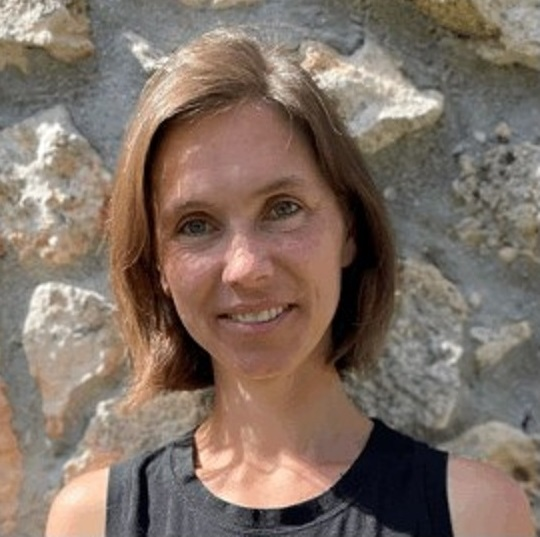
\includegraphics{author-bios/maria-pic.jpg}

\textbf{Maria Ruth Jones} co-founded and now leads DIME Analytics, an initiative to improve the quality, transparency, and reproducibility of empirical research. Her research interests center on survey methods, innovations in measurement, and technology adoption. She created and manages public goods to benefit the global research community, such as Development Research in Practice, the DIME Wiki, and the Manage Successful Impact Evaluations course. Maria joined the World Bank in 2009. Previous roles include coordination of the Global Agriculture and Food Security Program impact evaluation portfolio (2012--16) and a program of impact evaluations with the government of Malawi (2009--11).

\begin{center}\rule{0.5\linewidth}{0.5pt}\end{center}

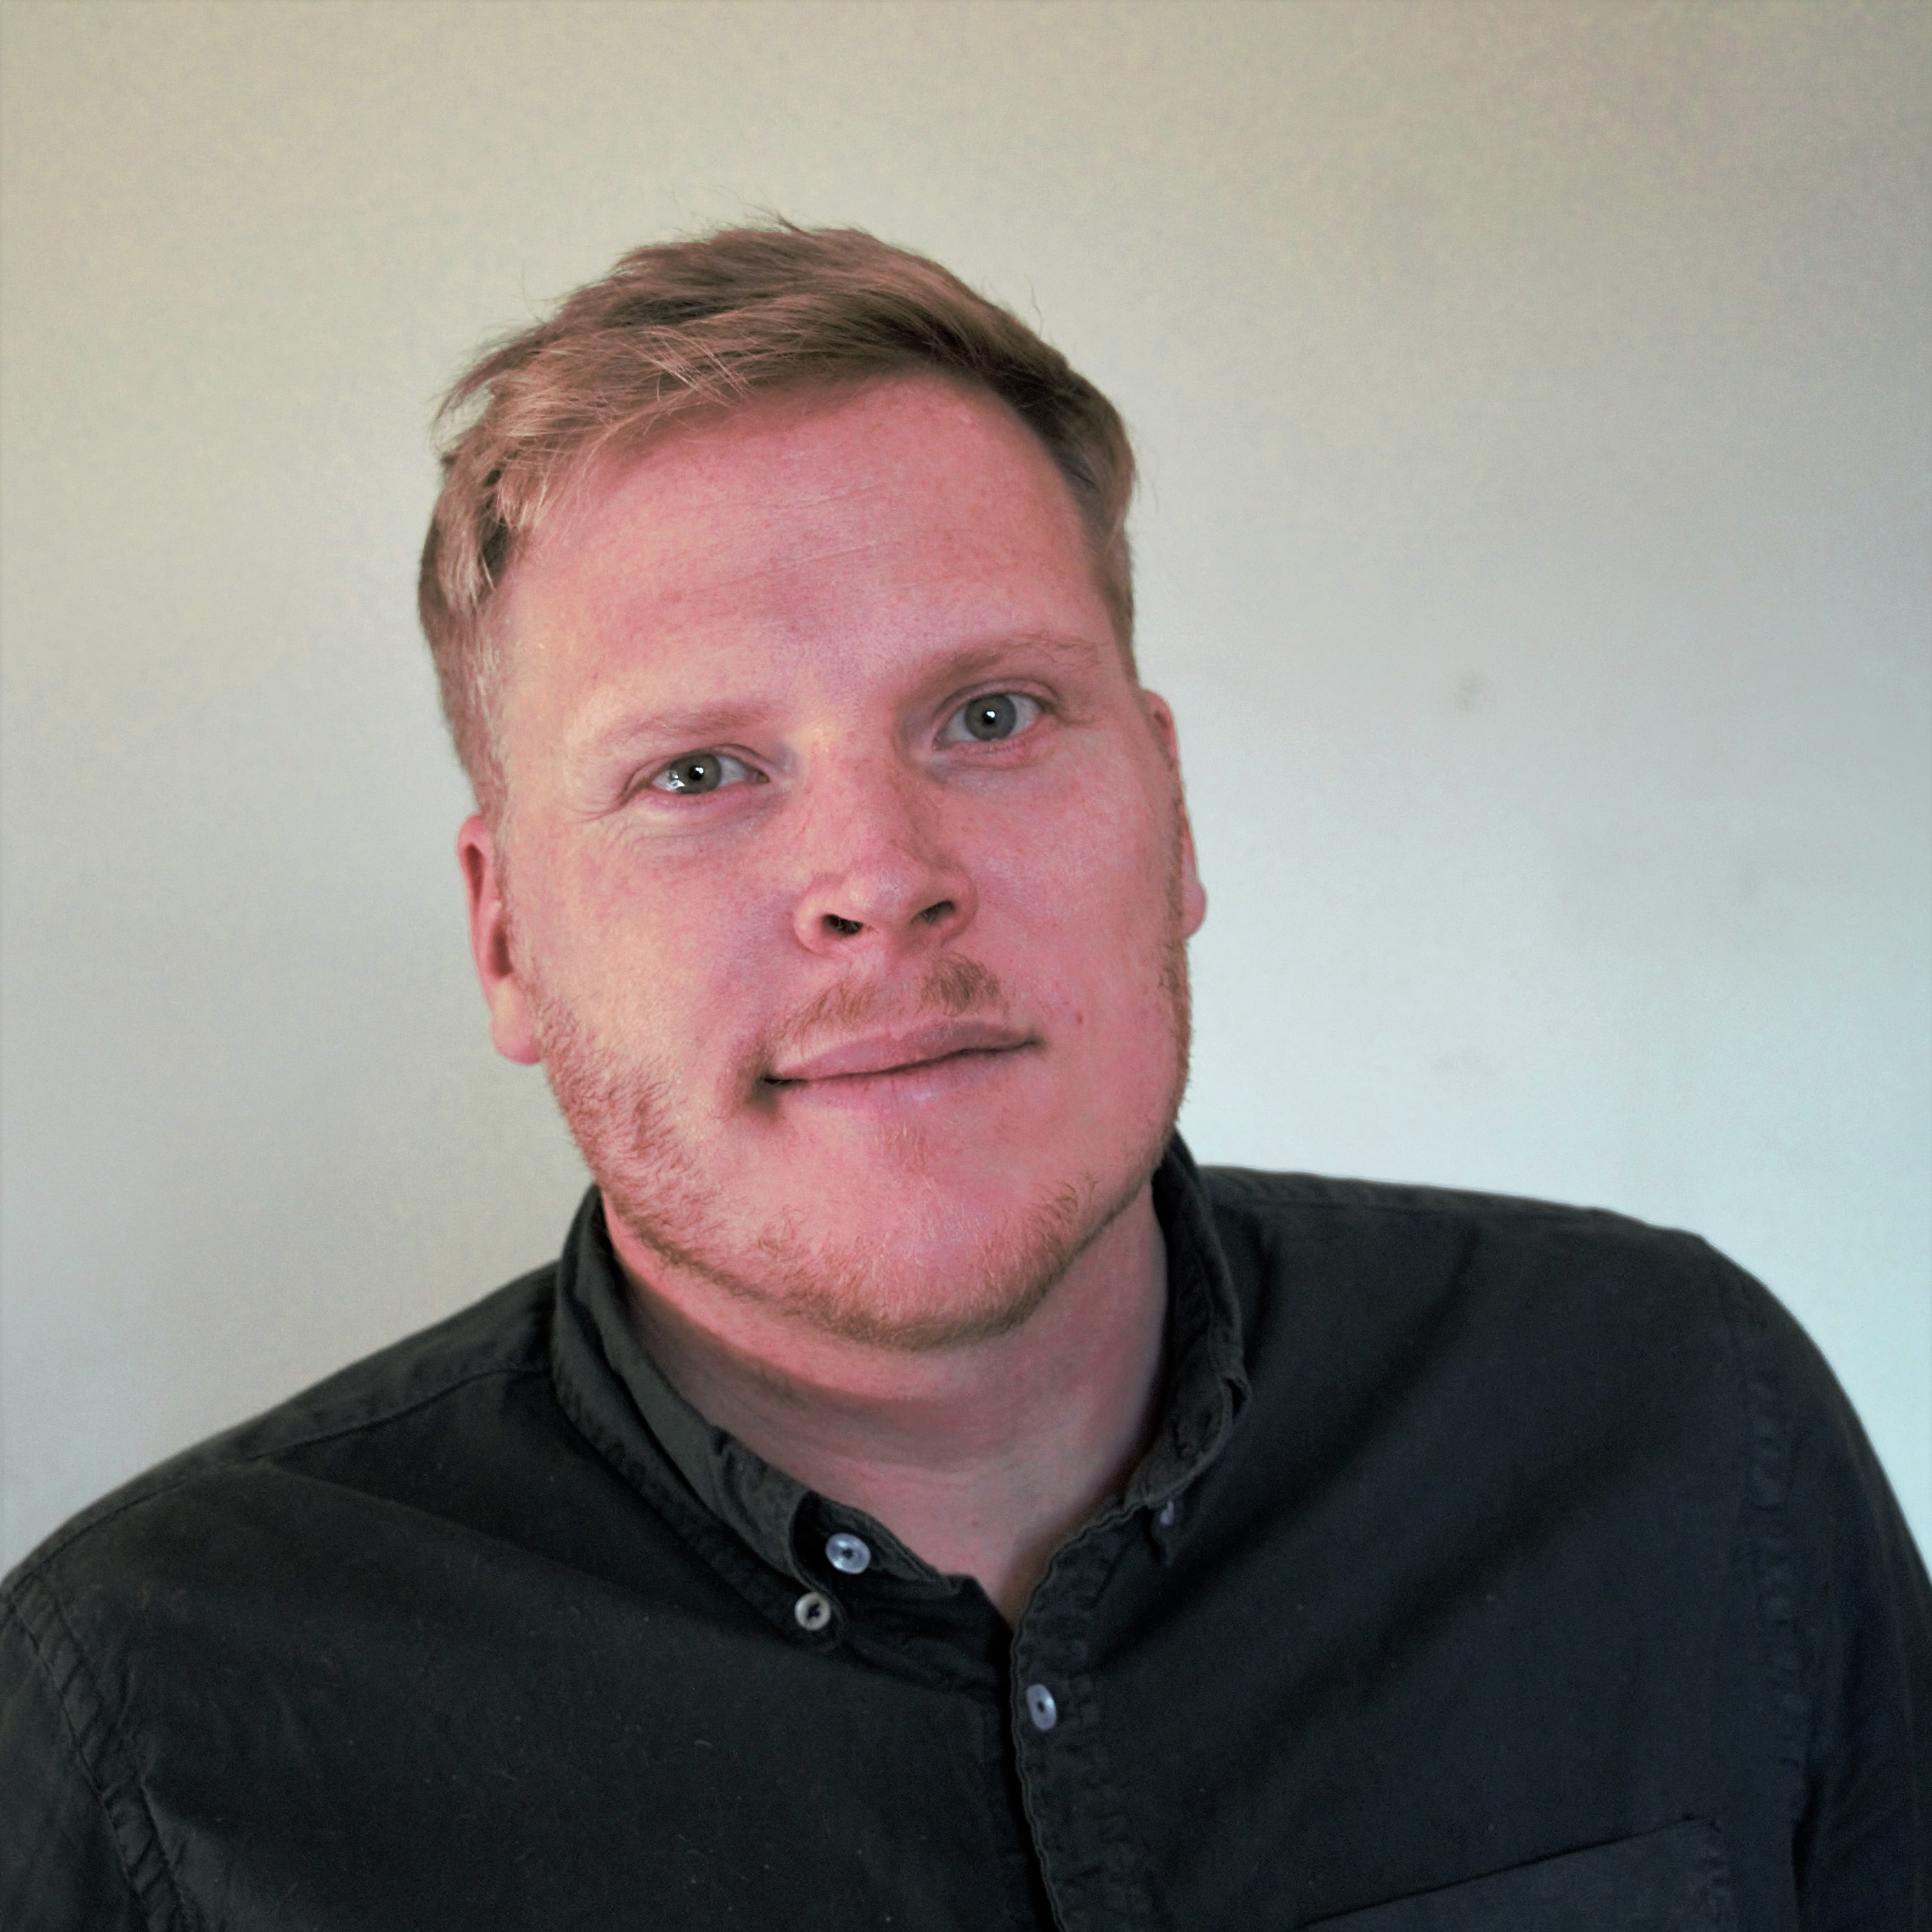
\includegraphics{author-bios/kristoffer-pic.jpg}

\textbf{Kristoffer Bjärkefur} is a Data Scientist Consultant with the Development Impact Evaluation department (DIME) at the World Bank Group. As a member of the DIME Analytics team, Kristoffer works to improve the reproducibility, transparency, and credibility of development research. He combines his backgrounds in development economics research and computer programming to make tools and best practices from the world of computer science more easily available to practitioners in development data. He supports teams in all stages in the life cycle of data and particularly enjoy planning data workflows. In DIME Analytics, he leads the work on data security and privacy.

\begin{center}\rule{0.5\linewidth}{0.5pt}\end{center}


\includegraphics{author-bios/luiza-pic.jpg}

\textbf{Luíza Cardoso de Andrade} is a Junior Data Scientist with the Development Impact Evaluation department (DIME) at the World Bank Group. Her work on the DIME Analytics team focuses on promoting research transparency and reproducibility practices through trainings and code review. She also works across DIME's portfolio of impact evaluations to incorporate non-traditional data sources such as high-frequency crowdsourced and web-scraped data. Luíza has also developed original software tools for research, including web-based data interfaces and the ietoolkit and iefieldkit Stata packages. Her research work has focused on agriculture, gender and environmental policy.

\begin{center}\rule{0.5\linewidth}{0.5pt}\end{center}


\includegraphics{author-bios/ben-pic.jpg}

\textbf{Benjamin Daniels} is a Fellow at the Georgetown University Initiative on Innovation, Development and Evaluation. His research focuses on the delivery of quality primary health care in developing contexts. His work has highlighted the importance of direct measurement of provider knowledge, effort, and practice. He has supported some of the largest research studies to date using clinical vignettes, provider observation, and standardized patients. Benjamin works with DIME Analytics to improve the transparency and credibility of development research. This work comprises research training and resources like the DIME Wiki and software products like iefieldkit and ietoolkit, among other Stata code tools.

\hypertarget{abbreviations}{%
\chapter*{Abbreviations}\label{abbreviations}}
\addcontentsline{toc}{chapter}{Abbreviations}

\textbf{2SLS} -- Two-Stage Least Squares

\textbf{AEA} -- American Economic Association

\textbf{CAPI} -- Computer-Assisted Personal Interviewing

\textbf{DD or DiD} -- Differences-in-Differences

\textbf{DDI} - Data Documentation Initiative

\textbf{DIME} -- Development Impact Evaluation

\textbf{DOI} -- Digital object identifier

\textbf{eGAP} -- Evidence in Governance and Politics

\textbf{EU} -- European Union

\textbf{FDE} - Full Disk Encryption

\textbf{FSE} - Full System Encryption

\textbf{GB} -- Gigabyte

\textbf{GDPR} -- Global Data Protection Regulation

\textbf{HFC} -- High-Frequency Checks

\textbf{IPA} -- Innovations for Poverty Action

\textbf{IRB} -- Institutional Review Board

\textbf{IV} -- Instrumental Variables

\textbf{J-PAL} -- The Abdul Latif Jameel Poverty Action Lab

\textbf{MB} -- Megabyte

\textbf{MDE} -- Minimum Detectable Effect

\textbf{NGO} -- Non-Governmental Organization

\textbf{ODK} -- Open Data Kit

\textbf{OLS} -- Ordinary Least Squares

\textbf{OSF} -- Open Science Framework

\textbf{PI} -- Principal Investigator

\textbf{PII} -- Personally-Identifying Information

\textbf{RA} -- Research Assistant

\textbf{RD} -- Regression Discontinuity

\textbf{RCT} -- Randomized Control Trial

\textbf{SSC} -- Statistical Software Components

\textbf{URL} - Uniform Resource Locator

\textbf{VPN} - Virtual Private Network

\hypertarget{preface}{%
\chapter{Preface}\label{preface}}

Welcome to \emph{Development Research in Practice: The DIME Analytics Data Handbook}. This book is intended to teach all users of development data how to handle data effectively, efficiently, and ethically. An empirical revolution has changed the face of development research rapidly over the last decade. Increasingly, researchers are working not just with complex data, but with \emph{original} data: datasets collected by the research team themselves or acquired through a unique agreement with a project partner. Research teams must carefully document how original data is created, handled, and analyzed. These tasks now contribute as much weight to the quality of the evidence as the research design and the statistical approaches do. At the same time, the scope and scale of empirical research projects is expanding: more people are working on the same data over longer timeframes. For that reason, the central premise of this book is that data work is a ``social process''. This means that the many different people on a team need to have the same ideas about what is to be done, and when and where and by whom, so that they can collaborate effectively on a large, long-term research project.

Despite the growing importance of managing data work, little practical guidance is available for practitioners. There are few guides to the conventions, standards, and best practices that are fast becoming a necessity for empirical research. \emph{Development Research in Practice} aims to fill that gap. It covers the full data workflow for a complex research project using original data. We share the lessons, tools, and processes developed within the World Bank's Development Impact Evaluation (DIME) department, and compile them into a single narrative of best practices for data work. This book is not sector-specific; it will not teach you econometrics, or how to design an impact evaluation. There are many excellent existing resources on those topics. Instead, it will teach you how to think about all aspects of your research from a data perspective, how to structure research projects to ensure data quality, and how to institute transparent and reproducible workflows. We realize that adopting these workflows may have significant upfront learning costs, but we are convinced that these investments pay off quickly, as you will both save time and improve the quality of your research going forward.

\hypertarget{how-to-read-this-book}{%
\section*{How to read this book}\label{how-to-read-this-book}}
\addcontentsline{toc}{section}{How to read this book}

This book aims to be a highly practical resource so the reader can immediately begin to collaborate more effectively on large, long-term research projects that use the methods and tools discussed. This introduction outlines the basic philosophies that motivate this book and our approach to research data. We want all readers to understand at the outset our mindset that research data work is primarily about communicating effectively within a team and that standardization and simplification of data tasks is a major enabler of effective collaboration. The main chapters of this book will walk you through the data workflow at each stage of an empirical research project, from design to publication. The figure in this introduction visualizes the data workflow. Chapters \ref{reproducibility} and \ref{collaboration} contextualize the workflow, and set the stage for the hands-on data tasks which are described in detail in Chapters \ref{measurement} to \ref{publication}.

\textbf{Chapter \ref{reproducibility}} This book aims to be a highly practical resource so the reader can immediately begin to collaborate more effectively on large, long-term research projects that use the methods and tools discussed. This introduction outlines the basic philosophies that motivate this book and our approach to research data. We want all readers to understand at the outset our mindset that research data work is primarily about communicating effectively within a team and that standardization and simplification of data tasks is a major enabler of effective collaboration. The main chapters of this book will walk you through the data workflow at each stage of an empirical research project, from design to publication. The figure in this introduction visualizes the data workflow. Chapters 1 and 2 contextualize the workflow, and set the stage for the hands-on data tasks which are described in detail in Chapters 3 to 7.

\textbf{Chapter \ref{collaboration}} teaches you to structure your data work for collaborative research, while ensuring the privacy and security of research participants. It discusses the importance of planning data work and associated tools in advance, long before any data is acquired. It also describes ethical concerns common to development data, common pitfalls in legal and practical management of data, and how to respect the rights of research participants at all stages of data work

\textbf{Chapter \ref{measurement}} turns to the measurement framework, and how to translate research design to a data work plan. It details DIME's data map template, a set of tools to communicate the project's data requirements both across the team and across time. It also discusses how to implement random sampling and random assignment in a reproducible and credible manner.

\textbf{Chapter \ref{acquisition}} covers data acquisition. It starts with the legal and institutional frameworks for data ownership and licensing, to ensure that you are aware of the rights and responsibilities of using data collected by the research team or by others. It provides a deep dive on collecting high-quality primary electronic survey data, including developing and deploying survey instruments. Finally, it discusses secure data handling during transfer, sharing, and storage, which is essential in protecting the privacy of respondents in any data.

\textbf{Chapter \ref{processing}} describes data processing tasks. It details how to construct ``tidy'' data at the appropriate units of analysis, how to ensure uniquely identified datasets, and how to routinely incorporate data quality checks into the workflow. It also provides guidance on de-identification and cleaning of personally-identified data, focusing on how to understand and structure data so that it is ready for indicator construction and analytical work.

\textbf{Chapter \ref{analysis}} discusses data analysis tasks. It begins with data construction, or the creation of new variables from the raw data acquired or collected in the field. It introduces core principles for writing analytical code and creating, exporting, and storing research outputs such as figures and tables reproducibly using dynamic documents.

\textbf{Chapter \ref{publication}} outlines the publication of research outputs, including manuscripts, code, and data. This chapter discusses how to effectively collaborate on technical writing using dynamic documents. It also covers how and why to publish datasets in an accessible, citable, and safe fashion. Finally, it provides guidelines for preparing functional and informative reproducibility packages that contain all the code, data, and meta-information needed for others to evaluate and reproduce your work.

Each chapter starts with a box which provides a summary of the most important points, takeaways for different types of readers, and a list of key tools and resources for implementing the recommended practices. After reading each chapter, you should understand what tasks will be performed at every stage of the workflow, and how to implement them according to best practices. You should also understand how the various stages of the workflow tie together, and what inputs and outputs are required and produced from each. The references and links contained in each chapter will lead you to detailed descriptions of individual ideas, tools, and processes to refer to when you need to implement the tasks yourself.

\begin{ex}
\hypertarget{demand-for-safe-spaces-case-study}{%
\subsection{Demand for Safe Spaces Case Study}\label{demand-for-safe-spaces-case-study}}

Throughout this Handbook, we will refer to a completed DIME project, \emph{Demand for Safe Spaces: Avoiding Harassment and Stigma}, to provide a case study of the empirical research tasks described in this book. You will find boxes in each chapter with examples of how the practices and workflows described in that chapter were applied in this real-life example. All the code examples and diagrams referenced in the case study can be accessed directly through this book's GitHub repository. We have made minor adaptations to the original study materials presented for function and clarity. All original materials can be found in the project's reproducibility package.

\textbf{The \emph{Demand for Safe Spaces} study is summarized in its abstract as follows.} What are the costs to women of harassment on public transit? This study randomizes the price of a women-reserved ``safe space'' in Rio de Janeiro and crowdsource information on 22,000 rides. Women in the public space experience harassment once a week. A fifth of riders are willing to forgo 20 percent of the fare to ride in the ``safe space''. Randomly assigning riders to the ``safe space'' reduces physical harassment by 50 percent, implying a cost of \$1.45 per incident. Implicit Association Tests show that women face a stigma for riding in the public space that may outweigh the benefits of the safe space.

The Demand for Safe Spaces study used novel original data from three sources. It collected information on 22,000 metro rides from a crowdsourcing app (referred to as \emph{crowdsourced ride data} in the case study examples), a survey of randomly-sampled commuters on the platform (referred to as the \emph{platform survey}), and data from an \emph{implicit association test}. The research team first elicited revealed preferences for the women-reserved cars, and then randomly assigned riders across the reserved and non-reserved cars to measure differences in the incidence of harassment. The use of a customized app allowed the researchers to assign data collection tasks and vary assigned ride spaces (women-reserved car vs public cars) and associated payout across rides. In addition, the team administered social norm surveys and implicit associations tests on a random sample of men and women commuters to document a potential side effect of reserved spaces: stigma against women who choose to ride in the public space.

For the purposes of the Handbook, we focus on the protocols, methods, and data used in the \emph{Demand for Safe Spaces study}, rather than the results. To learn more about the findings from this study, and more details on how it was conducted, we encourage readers to download the working paper.
The material from all the examples in the book and be found at \url{https://github.com/worldbank/dime-data-handbook/tree/master/examples}.

\begin{quote}
The Demand for Safe Spaces study repository can be accessed at \url{https://github.com/worldbank/rio-safe-space}.

The working paper \emph{Demand for Safe Spaces: Avoiding Harassment and Stigma} is available at \url{https://openknowledge.worldbank.org/handle/10986/33853}.
\end{quote}
\end{ex}

\hypertarget{the-dime-wiki-a-complementary-resource}{%
\section*{The DIME Wiki: A complementary resource}\label{the-dime-wiki-a-complementary-resource}}
\addcontentsline{toc}{section}{The DIME Wiki: A complementary resource}

Throughout the book, you will find many references to the DIME Wiki. The DIME Wiki is a free online collection of impact evaluation resources and best practices. This handbook and the DIME Wiki are meant to go hand-in-hand: the handbook provides the narrative structure and workflow, and the Wiki dives into specific implementation details, offers detailed code examples, and provides a more exhaustive set of references for each topic. Importantly, the DIME Wiki is a living resource that is continuously updated and improved, by the authors of this book and external contributors. We welcome all readers to \href{https://dimewiki.worldbank.org/New_Users}{register as Wiki users} and contribute directly.

\begin{figure}
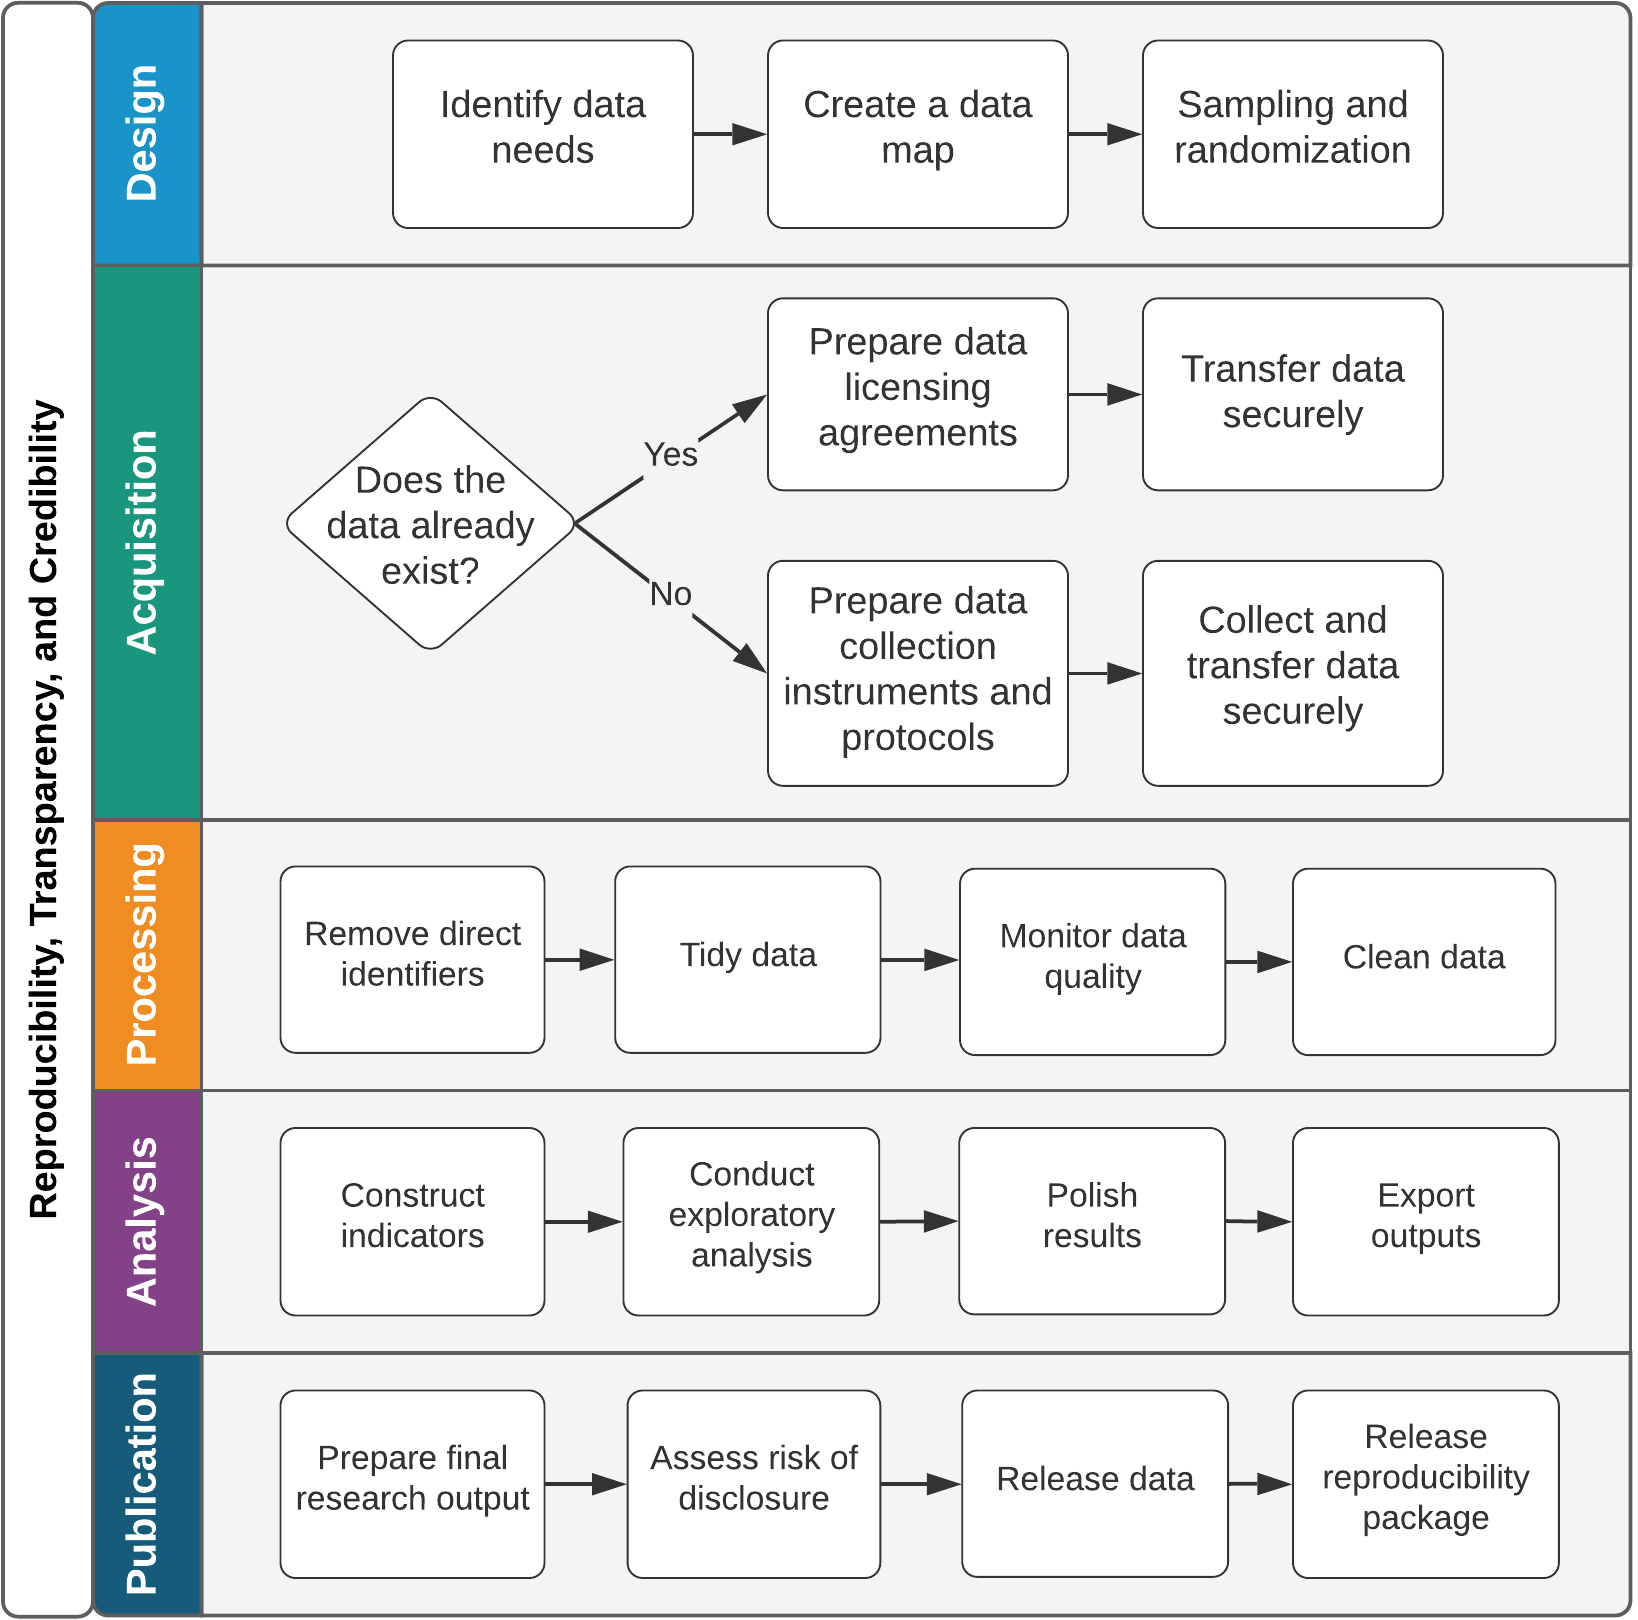
\includegraphics[width=22.75in]{diagrams/Introduction} \caption{Overview of development research data work tasks}\label{fig:unnamed-chunk-2}
\end{figure}

\hypertarget{standardizing-data-work}{%
\section*{Standardizing data work}\label{standardizing-data-work}}
\addcontentsline{toc}{section}{Standardizing data work}

In the past, data work was often treated as a ``black box'' in research.
A published manuscript might exhaustively detail
research designs, estimation strategies, and theoretical frameworks,
but typically reserved very little space for detailed descriptions
of how data was actually collected and handled.
It is almost impossible to assess the quality of the data in such a paper,
and whether the results could be reproduced.
In the past decade, this has started to change,\footnote{Swanson et al. (\protect\hyperlink{ref-swanson2020research}{2020})}
in part due to increasing requirements by publishers and funders to release code and data.

Data handling and documentation is a key skill for researchers and research staff.
Standard processes and documentation practices
are important throughout the research process to accurately convey
and implement the intended research design,\footnote{Vilhuber (\protect\hyperlink{ref-vilhuber_lars_2020_3911311}{2020})}
and to minimizes security risks:
better protocols and processes lower the probability of data leakages,
security breaches, and loss of personal information.
When data work is done in an ad-hoc manner,
it is very difficult for others to understand what is being done --
a reader has to simply trust that the researchers did these things right.
Most importantly, if any part of the data pipeline breaks down,
research results become unreliable\footnote{McCullough, McGeary, and Harrison (\protect\hyperlink{ref-mccullough2008economics}{2008})}
and cannot be faithfully interpreted
as being an accurate picture of the intended research design.\footnote{\url{https://blogs.worldbank.org/impactevaluations/more-replication-economics}}
Because we almost never have ``laboratory'' settings\footnote{See Baldwin and Mvukiyehe (\protect\hyperlink{ref-baldwin2015elections}{2015}) for an example.}
in this type of research,
such a failure has a very high cost:
we will have wasted the investments that were made into knowledge generation,
and the research opportunity itself,
where we intended to conduct the study.\footnote{Camerer et al. (\protect\hyperlink{ref-camerer2016evaluating}{2016})}

Accurate and reproducible data management and analysis
is essential to the success and credibility of modern research.
Standardizing and documenting data handling processes is essential
to be able to evaluate and understand
the data work alongside any final research outputs.
An important component of this is \textbf{process standardization}.\footnote{\textbf{Process standardization:} Agreement within a research team
  about how all tasks of a specific type will be approached.}\index{process standardization}
Process standardization means that there is
little ambiguity about how something ought to be done,
and therefore the tools to do it can be set in advance.
Standard processes help other people understand your work,
and they also make your work easier to document.
Process standardization and documentation should allow readers of your code to:
(1) quickly understand what a particular process or output is supposed to be doing;
(2) evaluate whether or not it does that thing correctly; and
(3) modify it either to test alternative hypotheses or to adapt into their own work.
This book will discuss specific standards recommended by DIME Analytics,
but we are more interested in convincing the reader
to discuss the adoption of \emph{a} standard within research teams
than to necessarily use \emph{the} particular standards that we recommend.

\hypertarget{standardizing-coding-practices}{%
\section*{Standardizing coding practices}\label{standardizing-coding-practices}}
\addcontentsline{toc}{section}{Standardizing coding practices}

Modern quantitative research relies heavily
on standardized statistical software tools,
written with various coding languages, to standardize analytical work.
Outputs like regression tables and data visualizations
are created using code in statistical software for two primary reasons.
The first is that using a standard command or package ensures that the work is done right,
and the second is that it ensures the same procedure can be confirmed or checked
at a later date or using different data.
Keeping a clear, human-readable record of these code and data structures is critical.
While it is often \emph{possible} to perform nearly all the relevant tasks
through an interactive user interface or even through software such as Excel,
this practice is strongly advised against.
In the context of statistical analysis,
the practice of writing all work using standard code is widely accepted.
To support this practice, DIME now maintains portfolio-wide standards
about how analytical code should be maintained and made accessible
before, during, and after release or publication.

Over the last few years, DIME has extended the same principles to preparing data for analysis,
which often comprises just as much (or more) of the manipulation done to the data
over the life cycle of a research project.
A major aim of this book is to encourage research teams
to think of the tools and processes they use
for designing, collecting, and handling data
just as they do for analytical tasks.
Correspondingly, a major contribution of DIME Analytics
has been tools and standard practices
for implementing these tasks using statistical software.

While we assume that you are going to do nearly all data work using code,
many development researchers come from economics and statistics backgrounds
and often understand code to be a means to an end rather than an output itself.
We believe that this must change somewhat:
in particular, we think that development practitioners
must think about their code and programming workflows
just as methodologically as they think about their research workflows,
and think of code and data as research outputs, just as manuscripts and briefs are.

This approach arises because we see the code as the ``recipe'' for the analysis.
The code tells others exactly what was done,
how they can do it again in the future,
and provides a roadmap and knowledge base for further original work.\footnote{Hamermesh (\protect\hyperlink{ref-hamermesh2007replication}{2007})}
Performing every task through written code
creates a record of every task you performed.\footnote{Ozier (\protect\hyperlink{ref-ozier2019replication}{2019})}
It also prevents direct interaction
with the data files that could lead to non-reproducible processes.\footnote{Chang and Li (\protect\hyperlink{ref-chang2015economics}{2015})}
Finally, DIME Analytics has invested a lot of time in developing code as a learning tool:
the examples we have written and the commands we provide
are designed to provide a framework for common practice
across the entire DIME team, so that everyone is able to
read, review, and provide feedback on the work of others
starting from the same basic ideas about how various tasks are done.

Most specific code tools have a learning and adaptation process,
meaning you will become most comfortable with each tool
only by using it in real-world work.
To support your process of learning reproducible tools and workflows,
we reference free and open-source tools wherever possible,
and point to more detailed instructions when relevant.
\textbf{Stata},\footnote{StataCorp, LLC (\protect\hyperlink{ref-statacorp2019stata}{2019})}
as a proprietary software, is the notable exception here
due to its persistent popularity in development economics and econometrics.
This book also includes, in Appendix \ref{coding},
the \textbf{DIME Analytics Coding Guide}
which includes instructions for how to write good code,
instructions on how to use the code examples in this book,
as well as our Stata Style Guide.
DIME projects are strongly encouraged to
explicitly adopt and follow coding style guides in their work.
Style guides harmonize code within and across teams
making it easier to understand and reuse code,
which ultimately helps teams to
build on each other's best practices.
Some of the programming languages used at DIME
already have well-established and commonly used style guides,
such as the Tidyverse style guide for R
and PEP-8 for Python.\footnote{See DIME Analytics Coding Standards:
  \url{https://github.com/worldbank/dime-standards}}.
Stata has relatively few resources of this type available,
which is why we have created and included one here that
we hope will be an asset to all Stata users.

\hypertarget{the-team-behind-this-book}{%
\section*{The team behind this book}\label{the-team-behind-this-book}}
\addcontentsline{toc}{section}{The team behind this book}

DIME is the Development Impact Evaluation department of the World Bank.\footnote{\url{https://www.worldbank.org/en/research/dime}}
Its mission is to generate high-quality and operationally relevant data and research
to transform development policy, help reduce extreme poverty, and secure shared prosperity.\footnote{Legovini, Di Maro, and Piza (\protect\hyperlink{ref-legovini2015impact}{2015})}
DIME develops customized data and evidence ecosystems to produce actionable information
and recommend specific policy pathways to maximize impact.
The department conduct research in 60 countries with 200 agencies, leveraging a
US\$180 million research budget to shape the design and implementation of
US\$18 billion in development finance.
DIME also provides advisory services to 30 multilateral and bilateral development agencies.\footnote{Legovini et al. (\protect\hyperlink{ref-legovini2019}{2019})}
DIME research is organized into four primary topic pillars:
Economic Transformation and Growth;
Gender, Economic Opportunity, and Fragility;
Governance and Institution Building;
and Infrastructure and Climate Change.
Over the years, DIME has employed dozens of research economists,
and hundreds of full-time research assistants, field coordinators, and other staff.
The team has conducted over 325 impact evaluations.
\emph{Development Research in Practice} exists to take advantage of that concentration and scale of research,
to synthesize many resources for data collection and research,
and to make DIME tools available to the larger community of development researchers.

As part of its broader mission, DIME invests in public goods
to improve the quality and reproducibility of development research around the world.
One key early innovation at DIME was the creation of
\href{https://www.worldbank.org/en/research/dime/data-and-analytics}{DIME Analytics},
the team responsible for writing and maintaining this book.
DIME Analytics is a centralized unit that develops and ensures adoption
of high quality research practices across the department's portfolio.
This is done through an intensive, collaborative innovation cycle:
DIME Analytics onboards and supports research assistants and field coordinators,
provides standard tools and workflows to all teams,
delivers hands-on support when new tasks or challenges arise,
and then develops and integrates lessons from those engagements to bring to the full team.
Resources developed and tested in DIME are converted into public goods
for the global research community, through open-access trainings and open-source tools.
Appendix \ref{resources}, the \textbf{DIME Analytics Resource Directory}, provides an introduction to public materials.

DIME Analytics has invested many hours over the past years
learning from data work across DIME's portfolio,
identifying inefficiencies and barriers to success,
developing tools and trainings, and standardizing best-practice workflows adopted in DIME projects.
It has also invested significant energy in the language and materials
used to teach these workflows to new team members,
and, in many cases, in software tools that support these workflows explicitly.
DIME team members often work on diverse portfolios of projects
with a wide range of teammates, and we have found
that standardizing core processes across all projects
results in higher-quality work with fewer opportunities to make mistakes.
In that way, the Analytics team is DIME's method of institutionalizing
tools and practices, developed and refined over time,
that give the department a common base of knowledge and practice.
In 2018, for example, DIME adopted universal reproducibility checks
conducted by the Analytics team;
the lessons from this practice helped move the DIME team
from where 50\% of submitted papers in 2018
required significant revision to pass
to where 64\% of papers passed in 2019 without revision required.

\hypertarget{looking-ahead}{%
\section*{Looking ahead}\label{looking-ahead}}
\addcontentsline{toc}{section}{Looking ahead}

While adopting the workflows and mindsets described in this book requires an up-front cost,
it will save you (and your collaborators) a lot of time and hassle very quickly.
In part this is because you will learn how to implement essential practices directly;
in part because you will find tools for the more advanced practices;
and most importantly because you will acquire the mindset of doing research with a high-quality data focus.

For some readers, the amount of new tools and practices recommended in this book may seem daunting.
We know from experience at DIME that full-scale adoption is possible;
in the last few years, the full DIME portfolio has transitioned to
transparent and reproducible workflows, with a fair share of hiccups along the way.
The authors of this book supported that at-scale transition,
and we hope that by sharing our lessons learned and resources,
the learning curve for readers will be less steep.
In the summary boxes at the beginning of each chapter,
we provide a list of the key tools and resources to help readers prioritize.
We will also offer ``second-best'' practices in many cases,
suggesting easy-to-implement suggestions to increase transparency and reproducibility,
in cases where full-scale adoption of the recommended workflows is not immediately feasible.
In fact, we encourage teams to adopt one new practice at a time
rather than rebuild their whole workflow from scratch right away.
We hope that by the end of the book,
all readers will have learned how to handle data more efficiently, effectively and ethically
at all stages of the research process.

\hypertarget{reproducibility}{%
\chapter{Conducting reproducible, transparent, and credible research}\label{reproducibility}}

Policy decisions are made every day using the results of development research,
and these have wide-reaching effects on the lives of millions.
As the emphasis on evidence-based policy grows,
so too does the scrutiny under which research methods and results are placed.
Three major components make up this scrutiny:
credibility, transparency, and reproducibility.
These three components contribute to one simple idea:
research should be high quality and well-documented.
Research consumers, including the policy makers who will use the evidence to make decisions,
should be able to easily examine and recreate such evidence.
In this framework, it is useful to think of research as a public service
that requires researchers as a group to be accountable for their methods.
This means acting to collectively protect the credibility of development research
by following modern practices for research planning and documentation.
Across the social sciences, the open science movement has been fueled
by concerns about the proliferation of low-quality research practices,
data and code that are inaccessible to the public,
analytical errors in major research papers,
and in some cases even outright fraud.
While the development research community has not yet
experienced major scandals,
it has become clear that there are necessary improvements to make
in the way that code and data are handled as part of research.
Moreover, having common standards and practices
for creating and sharing materials, code, and data with others
will improve the value of the work we do.

In this chapter, we outline principles and practices that help to ensure
research consumers can be confident in the conclusions reached.
We discuss each of the three components --
credibility, transparency, and reproducibility -- in turn.
The first section covers research credibility.
It presents three popular methods to commit to particular research questions or methods,
and avoid potential criticisms of cherry-picking results:
registration, pre-analysis plans, and registered reports.
The second section discusses how to apply principles of transparency to all research processes,
which allows research teams to be more efficient, and
research consumers to fully understand and evaluate research quality.
The final section provides guidance on how to make your research fully reproducible,
and explains why publishing replication materials is an important research contribution in its own right.

\begin{summary}
\hypertarget{summary-conducting-reproducible-transparent-and-credible-research}{%
\subsection*{Summary: Conducting reproducible, transparent, and credible research}\label{summary-conducting-reproducible-transparent-and-credible-research}}
\addcontentsline{toc}{subsection}{Summary: Conducting reproducible, transparent, and credible research}

This chapter describes three pillars of a high-quality empirical research project: credibility, transparency and reproducibility. These steps and outputs discussed in this chapter should be prepared at the beginning of a project and revisited through the publication process.

\textbf{1. Credibility:} to enhance credibility, you should pre-commit research decisions as much as feasible

\begin{itemize}
\tightlist
\item
  \emph{Register} research studies to provide a record of every project, so all evidence about a topic can be maintained; \emph{pre-register} studies to protect design choices from later criticism.
\item
  Write \emph{pre-analysis plans} to both strengthen the conclusions drawn from those analyses and increase efficiency by creating a road map for project data work.
\item
  Publish a \emph{registered report} to combine the benefits of the two steps above with a formal peer review process and a conditional acceptance of the final results of the specified research.
\end{itemize}

\textbf{2. Transparency:} you should document all data acquisition and analysis decisions during the project lifecycle, with a clear understanding of what will be released publicly and plan for how those will be published

\begin{itemize}
\tightlist
\item
  Develop and publish comprehensive \emph{project documentation}, especially instruments for data collection or acquisition that may be needed to prove ownership rights and facilitate re-use of the data.
\item
  Retain all \emph{original data} in an unaltered form and archive it appropriately, in preparation for it to be de-identified and published at the appropriate time.
\item
  Write all data processing and analysis \emph{code} with public release in mind.
\end{itemize}

\textbf{3. Reproducibility:} Prepare analytical work that can be verified and reproduced by others. This means

\begin{itemize}
\tightlist
\item
  Understanding what \emph{archives and repositories} are appropriate for your various materials
\item
  Preparing for \emph{legal documentation and licensing} of data, code, and research products
\item
  Initiating \emph{reproducible workflows} that will easily transfer within and outside of your research team and the necessary documentation for others to understand and use your materials
\end{itemize}

\hypertarget{takeaways}{%
\subsubsection*{Takeaways}\label{takeaways}}
\addcontentsline{toc}{subsubsection}{Takeaways}

\textbf{TTLs/PIs will:}

\begin{itemize}
\tightlist
\item
  Develop and document the research design and the corresponding data required to execute it
\item
  Guide the research team in structuring and completing project registration
\item
  Understand the team's future rights and responsibilities regarding data, code, and research publication
\item
  Determine what methods of pre-commitment are appropriate and lead the team in preparing them
\end{itemize}

\textbf{RAs will:}

\begin{itemize}
\tightlist
\item
  Rework outputs and documentation to meet specific technical requirements of registries, funders, publishers, or other governing bodies
\item
  Inform the team leadership whenever methodologies, data strategies, or their planned executions are not sufficiently clear or are not appropriately documented or communicated
\item
  Familiarize themselves with best practices for carrying out reproducible and transparent research, and initiate those practices within the research team
\end{itemize}

\hypertarget{key-resources}{%
\subsubsection*{Key Resources}\label{key-resources}}
\addcontentsline{toc}{subsubsection}{Key Resources}

\begin{itemize}
\tightlist
\item
  Register your research study: \url{https://dimewiki.worldbank.org/Study_Registration}
\item
  Create a pre-analysis plan: \url{https://dimewiki.worldbank.org/Pre-Analysis_Plan}
\item
  Prepare to document research decisions: \url{https://dimewiki.worldbank.org/Data_Documentation}
\item
  Publish data in a trusted repository: \url{https://dimewiki.worldbank.org/Publishing_Data}
\item
  Prepare and publish a reproducibility package: \url{https://dimewiki.worldbank.org/Reproducible_Research}
\end{itemize}
\end{summary}

\hypertarget{developing-a-credible-research-project}{%
\section*{Developing a credible research project}\label{developing-a-credible-research-project}}
\addcontentsline{toc}{section}{Developing a credible research project}

The evidentiary value of research is traditionally a function of design choices,\footnote{Angrist and Pischke (\protect\hyperlink{ref-angrist2010credibility}{2010}), Ioannidis (\protect\hyperlink{ref-ioannidis2005most}{2005})}
such as powered through sampling and randomization,
and robustness to alternative specifications and definitions.
One frequent target for critics of such research\footnote{Ioannidis, Stanley, and Doucouliagos (\protect\hyperlink{ref-ioannidis2017power}{2017})}
is the fact that most researchers have a lot of leeway
in selecting their projects, results, or outcomes
\emph{after} already having had the experience of implementing a project
or collecting data in the field,
which increases the likelihood of finding ``false positive''
results that are not true outside carefully-selected data.\footnote{Simmons, Nelson, and Simonsohn (\protect\hyperlink{ref-simmons2011false}{2011})}
Credible research design methods are key to maintaining credibility
in these choices and avoiding serious errors.
This is especially relevant for research that relies on original data sources,
from innovative big data sources to unique surveys.
Development researchers should take these concerns seriously.
Such flexibility can be a significant issue for the quality of evidence overall,
particularly if researchers believe that certain types of results
are substantially better for their careers or their publication chances.

This section presents three popular methods
for researchers to commit to particular research questions or methods,
and to avoid potential criticisms of cherry-picking results for publication:
registration, pre-analysis plans, and registered reports.\index{registration}\index{pre-analysis plans}\index{registered reports}
Each of these methods involves documenting specific research design components,
ideally before carrying out the analytical component or extensively exploring the data.
Study registration provides formal notice that a study is being attempted
and creates a hub for materials and updates about the study results.
Pre-analysis plans are a more formal commitment
to use specific methods on particular questions.
Writing and releasing a pre-analysis plan
in advance of working with data is used to protect the credibility
of approaches that have a high likelihood of producing false results.\footnote{Wicherts et al. (\protect\hyperlink{ref-wicherts2016degrees}{2016})}
Finally, registered reports allow researchers to approach research planning itself
as a process at the level of a full peer review.
Registered reports enable close scrutiny of a research design,
a feedback and improvement process,
and a commitment from a publisher to publish the study
based on the credibility of the design, rather than the specific results.

\hypertarget{registering-research-studies}{%
\subsection*{Registering research studies}\label{registering-research-studies}}
\addcontentsline{toc}{subsection}{Registering research studies}

Registration of research studies is an increasingly common practice,
and more journals are beginning to require
the registration of studies they publish.\footnote{Vilhuber, Turrito, and Welch (\protect\hyperlink{ref-vilhuber2020report}{2020})}
Study registration intended to ensure that a complete record of research inquiry is easily available.\footnote{More details on study registrations and
  links to additional resources can be found on the DIME Wiki:
  \url{https://dimewiki.worldbank.org/Study_Registration}}
Registering research studies ensures that future scholars can quickly
find out what work has been carried out on a given question,
even if some or all of the work done never results in formal publication.
Registration of studies is increasingly required by publishers
and can be done before, during, or after the study
with essential information about the study purpose.
Some currently popular registries are operated by the
\textbf{AEA},\footnote{\url{https://www.socialscienceregistry.org}}
\textbf{3ie},\footnote{\url{https://ridie.3ieimpact.org}}
\textbf{eGAP},\footnote{\url{https://egap.org/content/registration}}
and \textbf{OSF}\footnote{\url{https://osf.io/registries}}.
They all have different target audiences and features,
so select one that is appropriate to your work.
Study registration should be feasible for all projects,
as registries are typically free to access and can be initially submitted with minimal information about the project.
A generally-acceptable practice will be to gradually revise and expand the level of detail in a registration over time,
adding more information as the planning for the project progresses.
\index{pre-registration}

Pre-registering studies before they begin is an extension of this principle.\footnote{Nosek et al. (\protect\hyperlink{ref-nosek2018preregistration}{2018})}
Registration of a study before it goes to implementation or data acquisition,
particularly when specific hypotheses are included in the registration,
provides a simple and low-effort way for researchers
to conclusively demonstrate that a particular line of inquiry
was not generated by the process of data collection or analysis itself.\footnote{More details on how to pre-register your study
  and links to other resources can be found on the DIME Wiki:
  \url{https://dimewiki.worldbank.org/Pre-Registration}}\index{pre-registration}
Pre-registrations need not provide exhaustive details about how
a particular hypothesis will be approached; only that it will be.
Pre-registering specific individual elements of research design or analysis
can be highly valuable for the credibility of the research
and requires only minor time investment or administrative effort.
For this reason, the DIME team requires pre-registration of all studies
in a public database with at least some primary hypotheses prespecified,
prior to providing funding for impact evaluation research.

\begin{ex}
\hypertarget{demand-for-safe-spaces-case-study-registering-research-studies}{%
\subsection{Demand for Safe Spaces Case Study: Registering Research Studies}\label{demand-for-safe-spaces-case-study-registering-research-studies}}

The experimental component of the \emph{Demand for Safe Spaces} study was registered at the Registry for International Development Impact Evaluations (RIDIE) under ID 5a125fecae423.

Highlights from the Registry:

\begin{itemize}
\tightlist
\item
  \emph{Indicated evaluation method:} both primary method (randomized control trial) and additional methods (difference-in-difference/fixed effects).
\item
  \emph{Listed key outcome variables:} take-up of rides in women-only car (binary), occurrence of harassment or crime during ride (binary), self-reported well-being after each ride, overall subjective well-being, Implicit Association Test D-Score
\item
  \emph{Specified primary hypotheses to be tested:} The women-only car reduces harassment experienced by women who ride it; Riding the women's-only car improves psychological well-being of those who ride it; Women are willing to forego income to ride the women's-only car
\item
  \emph{Specified secondary research question and methods:} supplementary research methods (implicit association test and platform survey) to help address an additional hypothesis: The women's-only car is associated with a social norm that assigns responsibility to women for avoiding harassment.
\item
  \emph{Provided sample size for each study arm:} number of individual participants, number of baseline rides, number of rides during price experiment, number of car-assigned rides, number of expected participants in implicit association test
\item
  *Described data sources: the study relied on data previously collected (through the mobile app) and data to-be-collected (through platform surveys and implicit association tests)
\item
  \emph{Registration status:} categorized as a non-prospective registry, as the crowdsourced data had already been received and processed. It was important to the team to ensure the credibility of additional data collection and secondary research questions by registering the study.
\end{itemize}

\begin{quote}
The RIDIE registry can be accessed at \url{https://ridie.3ieimpact.org/index.php?r=search/detailView\&id=588}
\end{quote}
\end{ex}

\hypertarget{writing-pre-analysis-plans}{%
\subsection*{Writing pre-analysis plans}\label{writing-pre-analysis-plans}}
\addcontentsline{toc}{subsection}{Writing pre-analysis plans}

If a research team has a large amount of flexibility
to define how they approach a particular hypothesis,
study registration may not be sufficient to avoid the criticism of
``hypothesizing after the results are known'', or HARKing.\footnote{Kerr (\protect\hyperlink{ref-kerr1998harking}{1998})}
Examples of such flexibility include a broad range
of concrete measures that could be argued to measure to an abstract concept;
future choices about sample inclusion or exclusion;
or decisions about how to construct derived indicators.
There are a variety of templates and checklists of details to include.\footnote{We recommend this checklist:
  \url{https://blogs.worldbank.org/impactevaluations/a-pre-analysis-plan-checklist}}
When the researcher is collecting a large amount of information
and has leverage over even a moderate number of these options,
it is almost guaranteed that they can come up with any result they like.\footnote{Gelman and Loken (\protect\hyperlink{ref-gelman2013garden}{2013})}

Pre-analysis plans (PAPs) can be used to assuage these concerns
by specifying some set of analyses the researchers intend to conduct.\footnote{More details on how to prepare a pre-analysis plans
  and links to additional resources
  can be found on the DIME Wiki:
  \url{https://dimewiki.worldbank.org/Pre-Analysis_Plan}}\index{pre-analysis plan}
The pre-analysis plan should be written up in detail
for areas that are known to provide a large amount of leeway
for researchers to make later decisions,
particularly for things like interaction effects or subgroup analysis.\footnote{See Cusolito, Dautovic, and McKenzie (\protect\hyperlink{ref-cusolito2018can}{2018}) for an example.}
Pre-analysis plans shoud not, however, be viewed as binding the researcher's hands.\footnote{Olken (\protect\hyperlink{ref-olken2015promises}{2015})}
Depending on what is known about the study at the time of writing,
pre-analysis plans can vary widely in the amount of detail they should include.\footnote{\url{https://blogs.worldbank.org/impactevaluations/pre-analysis-plans-and-registered-reports-what-new-opinion-piece-does-and-doesnt}}
The core function of a PAP is to carefully and explicitly describe
one or more specific data-driven inquiries,
as specific formulations are often very hard to justify in retrospect
with data or projects that potentially provide many avenues to approach
a single theoretical question.\footnote{See Bedoya et al. (\protect\hyperlink{ref-bedoya2019no}{2019}) for an example.}
Anything outside the original plan is just as interesting and valuable
as it would have been if the plan was never published;
but having pre-committed to the details of a particular inquiry makes its results
immune to a wide range of criticisms of specification searching or multiple testing.\footnote{Duflo et al. (\protect\hyperlink{ref-duflo2020praise}{2020})}

\begin{ex}
\hypertarget{demand-for-safe-spaces-case-study-writing-pre-analysis-plans}{%
\subsection{Demand for Safe Spaces Case Study: Writing Pre-Analysis Plans}\label{demand-for-safe-spaces-case-study-writing-pre-analysis-plans}}

Although the \emph{Demand for Safe Spaces} study did not publish a formal pre-analysis plan, the team published a concept note in 2015, which includes much of the same information as a typical pre-analysis plan. The Concept Note was updated in May 2017 to include new secondary research questions. The Concept Note, prepared before fieldwork began, was subject to review and approval within the World Bank and from a technical committee including blinded feedback from external academics. The Concept Note specified the planned study along the following dimensions:

\begin{itemize}
\tightlist
\item
  \emph{Theory of change:} the main elements of the intervention, and the hypothesized causal chain from inputs, through activities and outputs, to outcomes.
\item
  \emph{Hypotheses} derived from the theory of change
\item
  \emph{Main evaluation question(s)} to be addressed by the study
\item
  \emph{List of main outcomes of interest,} including outcome name, definition, level of measurement
\item
  \emph{Evaluation design,} including a precise description of the identification strategy for each research questions and description of treatment and control groups
\item
  \emph{Sampling strategy and sample size calculation,} detailing the assumptions made
\item
  \emph{Description of all quantitative data collection instruments}
\item
  \emph{Data processing and analysis:} the statistical methods to be used, the exact specification(s) to be run, including clustering of standard errors; key groups for heterogeneity analysis; adjustments for multiple hypothesis testing; strategy to test (and correct) for bias.
\end{itemize}

\begin{quote}
A version of the study's Concept Note is available at \url{https://github.com/worldbank/rio-safe-space/blob/master/Online\%20Appendices/Supplemental\%20Material/Project\%20Concept\%20Note.pdf}
\end{quote}
\end{ex}

\hypertarget{publishing-registered-reports}{%
\subsection*{Publishing registered reports}\label{publishing-registered-reports}}
\addcontentsline{toc}{subsection}{Publishing registered reports}

\textbf{Registered reports} take the process of pre-specifying a complex research design
to the level of a formal publication.\footnote{More details on registered reports and
  links to additional resources can be found on the DIME Wiki:
  \url{https://dimewiki.worldbank.org/Registered_Reports}}\index{registered reports}
In a registered report, a journal or other publisher
will peer review and conditionally accept a specific study for publication,
typically then guaranteeing the acceptance of a later publication
that carries out the analysis described in the registered report.
While far stricter and more complex to carry out than
ordinary study registration or pre-analysis planning,
the registered report has the added benefit
of peer review and expert feedback
on the design and structure of the proposed study.\footnote{\url{https://blogs.worldbank.org/impactevaluations/registered-reports-piloting-pre-results-review-process-journal-development-economics}}
Registered reports are never required,
but they are designed to reward researchers
who are able to provide a large amount of advance detail for their projects,
researchers who want to secure publication interest regardless of results,
or researchers who want to use methods that may be novel or unusual.

This process is in part meant to combat the ``file-drawer problem''\footnote{Simonsohn, Nelson, and Simmons (\protect\hyperlink{ref-simonsohn2014p}{2014})}\index{file-drawer problem}
and ensure that researchers are transparent in the sense that
all promised results obtained from registered-report studies are actually published.
This approach has the advantage of pre-specifying in great detail
a complete research and analytical design,
and securing a commitment for publication regardless of the outcome.
This may be of special interest for researchers
studying events or programs where either there is a substantial risk
that they would either not be able to publish a null or negative result,\footnote{See Coville et al. (\protect\hyperlink{ref-coville2019nollywood}{2019}) for an example.}\index{null result}
or where they may wish to avoid any pressure toward finding a particular result,
for example when the program or event is the subject of substantial social or political pressures.
As with pre-registration and pre-analysis,
nothing in a registered report should be understood
to prevent a researcher from pursuing additional avenues of inquiry
once the study is complete, either in the same or separate research outputs.

\hypertarget{conducting-research-transparently}{%
\section*{Conducting research transparently}\label{conducting-research-transparently}}
\addcontentsline{toc}{section}{Conducting research transparently}

Transparent research exposes not only the code,
but all research processes involved in developing the analytical approach.
This means that readers are able to judge for themselves whether the research was done well
and the decision-making process was sound.
If the research is well-structured, and all of the relevant documentation\footnote{More details on research documentation and
  links to additional resources can be found on the DIME Wiki:
  \url{https://dimewiki.worldbank.org/Research_Documentation}}\index{research documentation}
is shared, it is easy for the reader to understand the analysis fully.
Researchers that expect process transparency also have an incentive to make better decisions,
be skeptical and thorough about their assumptions,
and save themselves time,
because transparent research methods are labor-saving over the complete course of a project.

Clearly documenting research work is necessary
to allow others to evaluate exactly what data was acquired and how it was used
to obtain a particular result.
Many development research projects are purpose-built
to address specific questions,
and often use unique data, novel methods, or small samples.
These approaches can yield new insights into essential academic questions,
but need to be transparently documented so they can be reviewed
or replicated by others in the future.\footnote{Duvendack, Palmer-Jones, and Reed (\protect\hyperlink{ref-duvendack2017meant}{2017})}
Unlike disciplines where data is more standardized
or where research is more oriented around secondary data,
the exact data used in a development project
has often not been observed by anyone else in the past
and may not be able to be re-collected by others in the future.
Regardless of the novelty of study data,
transparent documentation methods help ensure
that data was collected and handled appropriately
and that studies and interventions were implemented correctly.
As with study registrations, project and data documentation
should be released on external \textbf{archival repositories}\footnote{\textbf{Archival repository:} A third-party service for information storage
  that guarantees the permanent availability of current and prior versions of materials.}\index{archival repository}
so they can always be accessed and verified.

\hypertarget{documenting-data-acquisition-and-analysis}{%
\subsection*{Documenting data acquisition and analysis}\label{documenting-data-acquisition-and-analysis}}
\addcontentsline{toc}{subsection}{Documenting data acquisition and analysis}

Documenting a project in detail greatly increases transparency.
Many disciplines have a tradition of keeping a ``lab notebook'',
and adapting and expanding this process to create a
lab-style workflow in the development field is a
critical step towards more transparent practices.
This means explicitly noting decisions as they are made,
and explaining the process behind the decision-making.
Careful documentation will also save the research team a lot of time during a project,
as it prevents you from having the same discussion twice (or more!),
since you have a record of why something was done in a particular way.
There are a number of available tools
that will contribute to producing documentation,\index{project documentation}
but project documentation should always be an active and ongoing process,
not a one-time requirement or retrospective task.
New decisions are always being made as the plan begins contact with reality,
and there is nothing wrong with sensible adaptation so long as it is recorded and disclosed.

Email, however, is \emph{not} a documentation service, because communications are rarely well-ordered,\index{email}
can be easily deleted, and are not available for future team members.
At the very least, emails and other decision-making communications
need to be archived and preserved (as, say, PDFs)
in an organized manner so that they can be easily accessed and read by others in the future.
There are also various software solutions for building proper documentation over time.
Some work better for field records such as implementation decisions,
research design, and survey development;
others work better for recording data work and code development.
The \textbf{Open Science Framework}\footnote{\url{https://osf.io}} provides one such solution,\index{Open Science Framework}
with integrated file storage, version histories, and collaborative wiki pages.
\textbf{GitHub}\footnote{\url{https://github.com}} provides a transparent documentation system
through commit messages, issues, \texttt{README} files, and pull requests,\footnote{More details on how to use Git and GitHub and links to all DIME Analytics
  resources on best practices and how to get started can be found on the DIME Wiki:
  \url{https://dimewiki.worldbank.org/Getting_started_with_GitHub}}\index{task management}\index{GitHub}\index{README}
in addition to version histories and wiki pages.\index{version control}
Such services offer multiple different ways
to record the decision process leading to changes and additions,
track and register discussions, and manage tasks.
These are flexible tools that can be adapted to different team and project dynamics.
Services that log your research process can show things like modifications made in response to referee comments,
by having tagged version histories at each major revision.
They also allow you to use issue trackers
to document the research paths and questions you may have tried to answer
as a resource to others who have similar questions.
Each project has specific requirements for data, code, and documentation management,
and the exact transparency tools to use will depend on the team's needs,
but they should be agreed upon prior to project launch.
This way, you can start building a project's documentation as soon as you start making decisions.

\hypertarget{cataloging-and-archiving-data}{%
\subsection*{Cataloging and archiving data}\label{cataloging-and-archiving-data}}
\addcontentsline{toc}{subsection}{Cataloging and archiving data}

Data and data collection methods should be fully cataloged, archived, and documented,
whether you are collecting data yourself or receiving it from an outside partner.
In some cases this is as simple as uploading
a survey instrument or an index of datasets and a codebook to an archive.\index{codebook}
In other cases this will be more complex.
Proper documentation of data collection will often require
a detailed description of the overall sampling procedure.\footnote{See Yishay et al. (\protect\hyperlink{ref-yishay2016gender}{2016}) for an example.}
For example, settings with many overlapping strata,
treatment arms, excluded observations, or resampling protocols
might require extensive additional field work documentation.
This documentation should be continuously updated
and kept with the other study materials;
it is often necessary to collate these materials
for an appendix for publication in any case.

When data is received from partners or collected in the field,
the \textbf{original data} (including corrections)\footnote{\textbf{Original data:} A new dataset, as obtained and corrected,
  that becomes the functional basis for research work.}\index{original data}
should be immediately placed in a secure permanent storage system.
Before analytical work begins, you should create a ``for-publication''
copy of the original dataset by removing potentially identifying information.\index{de-identification}
This will become the raw data, and must be
placed in an archival repository where it can be cited.\footnote{Vilhuber, Turrito, and Welch (\protect\hyperlink{ref-vilhuber2020report}{2020})}\index{data publication}
This can initially be done under embargo or with limited release,
in order to protect your data and future work.
This type of data depositing or archiving
precedes publishing or releasing any data:
data at this stage may still need to be embargoed
or have other, potentially permanent, access restrictions,
so you can instruct the archive to formally release the data later.
If your planned analysis requires the use of unpublishable data,
that data should always remain encrypted and be stored separately
so it is clear what portions of the code will work with and without
obtaining a license to the needed restricted-access data.

Some project funders
provide specific repositories in which they require the deposit of data they funded,\footnote{For example, \url{https://data.usaid.gov}}
and you should take advantage of these when possible.
If this is not provided, you must be aware of privacy issues
with directly identifying data and questions of data ownership
before uploading raw data to any third-party server, whether public or not;\index{data ownership}
this is a legal question for your home organization.
If data that is required for analysis must be placed under restricted use or restricted access,
including data that can never be distributed directly by you to third parties,
develop a plan for storing that data separately from publishable information.
This will allow you to maximize transparency by having a clear release package
as well as providing instructions or developing a protocol for allowing access in the future
for replicators or reviewers under appropriate access agreements.\footnote{Details on how to document this type of material can be found at
  \url{https://doi.org/10.5281/zenodo.4319999}.}
Regardless of these consideration, all data repositories,
such as DIME's standard, the World Bank Microdata Library\footnote{\url{https://microdata.worldbank.org}}
and the World Bank Data Catalog,\footnote{\url{https:/datacatalog.worldbank.org}}
should create a record of the data's existence
and provide instructions on how access might be obtained by another researcher.
For more on the steps required to prepare and publish a de-identified dataset,
you can refer to chapters \ref{analysis} and \ref{publication} of this book.
Data publication should create a data citation and a \textbf{digital object identifier (DOI)},\footnote{\textbf{Digital object identifier (DOI):} A permanent reference for electronic information
  that persistently updates to a new URL or other locations if the information is relocated.}\index{digital object identifier (DOI)}\index{data citation}
or some other persistent index that you can use in your future work
to unambiguously indicate the location of your data.
This data publication should also include the methodological documentation
as well as complete human-readable codebooks for all the variables there.

\hypertarget{analyzing-data-reproducibly}{%
\section*{Analyzing data reproducibly}\label{analyzing-data-reproducibly}}
\addcontentsline{toc}{section}{Analyzing data reproducibly}

Reproducible research makes it easy
for others to apply your techniques to new data
or to implement a similar research design in a different context.
Development research is rapidly moving in the direction of requiring adherence
to specific reproducibility guidelines.\footnote{Christensen and Miguel (\protect\hyperlink{ref-christensen2018transparency}{2018})}
Major publishers and funders, most notably the American Economic Association,
have taken steps to require that code and data
are accurately reported, cited, and preserved as research outputs
that can be accessed and verified by others.
Making research reproducible in this way is a public good.\footnote{More details and links to additional resources on
  how to make your research reproducible and prepare a reproducibility package
  can be found on the DIME Wiki:
  \url{https://dimewiki.worldbank.org/Reproducible_Research}.
  More details can also be found under Pillar 3 in the DIME Research Standards:
  \url{https://github.com/worldbank/dime-standards}.}
It enables other researchers to re-use code and processes
to do their own work more easily and effectively in the future.
Regardless of what is formally required,
your code should be written neatly with clear instructions.
It should be easy to read and understand.
The corresponding analysis data should also be made accessible
to the greatest legal and ethical extent that it can be.\footnote{More details and links to best practices on topics related to data publication,
  such as de-identification and how to license published data,
  can be found on the DIME Wiki:
  \url{https://dimewiki.worldbank.org/Publishing_Data}.
  More details can also be found under Pillar 5 in the DIME Research Standards:
  \url{https://github.com/worldbank/dime-standards}}

Common research standards from journals and funders feature both
regulation and verification policies.\footnote{Stodden, Guo, and Ma (\protect\hyperlink{ref-stodden2013toward}{2013})}
Regulation policies require that authors
provide reproducibility packages before publication
which are then reviewed by the journal for completeness.\footnote{The DIME Analytics reproducibility checklist can be found in Pillar 3 of
  the DIME Research Standards at \url{https://github.com/worldbank/dime-standards}.}
Verification policies require that authors
make certain materials available to the public,
but their completeness is not a precondition for publication.
Other journals have adopted guidance that offer checklists
for reporting on whether and how various practices were implemented,
without specifically requiring any.\footnote{Nosek et al. (\protect\hyperlink{ref-nosek2015promoting}{2015})}
If you are personally or professionally motivated by citations,
producing these kinds of resources can lead to that as well.
Even if privacy considerations mean
you will not be publishing some or all data or results,
these practices are still valuable for project organization.

Our recommendation, regardless of external requirements,
is that your should prepare to release all data that can be published
When data cannot be published, you should try to publish as much metadata as allowed,
including information on how the data was obtained,
what fields the data contains and aggregations or descriptive statistics.
Even if the data cannot be published,
it is rare for code files to contain restricted information,
so the code should still be made available with clear instructions for obtaining usable data.
Additionally, we recommend that reproducibility efforts be considered
when designing the IRB and data licensing agreement for sensitive data,
to establish acceptable conditions (such as a secure transfer or cold room)
under which representatives from journals or other academics could access data
may access the data for the purpose of independently reproducing results.

\hypertarget{preparing-a-reproducibility-package}{%
\subsection*{Preparing a reproducibility package}\label{preparing-a-reproducibility-package}}
\addcontentsline{toc}{subsection}{Preparing a reproducibility package}

At DIME, all research outputs are required to satisfy \textbf{computational reproducibility},\footnote{\textbf{Computational reproducibility:} The ability of another individual
  to reuse the same code and data and obtain the exact same results as yours.}\index{computational reproducibility}
which is an increasingly common requirement for publication.\footnote{More details and links to additional resources on
  how to make your research reproducible and prepare a reproducibility package
  can be found on the DIME Wiki:
  \url{https://dimewiki.worldbank.org/Reproducible_Research}.
  More details can also be found under Pillar 3 in the DIME Research Standards:
  \url{https://github.com/worldbank/dime-standards}.}
Before releasing a working paper,
the research team submits a \textbf{reproducibility package} with de-identified data,\index{reproducibility package}
and DIME Analytics verifies that the package produces
exactly the same results that appear in the paper.\footnote{\url{https://blogs.worldbank.org/impactevaluations/what-development-economists-talk-about-when-they-talk-about-reproducibility}}
The team also comments on whether the package includes sufficient documentation.
The Analytics team organizes frequent peer code review for works in progress,\index{code review}
and our general recommendation is to ensure that projects
are \emph{always} externally reproducible
instead of waiting until the final stages to prepare this material.
Once the computational reproducibility check is complete,
the team receives a completed reproducibility certificate
that also lists any publicly available materials to accompany the package,
for use as an appendix to the publication.
The team also organizes regular peer code review for works in progress,
and our general recommendation is to ensure that projects
are \emph{always} externally reproducible
instead of waiting until the final stages to prepare this material.
In this way, code is continuously maintained with clear documentation,
and should be easy to read and understand in terms of structure, style, and syntax.

For research to be reproducible,
all code files for data cleaning, construction and analysis
should be public, unless they contain confidential information.
Nobody should have to guess what exactly comprises a given index,
or what controls are included in your main regression,
or whether or not you clustered standard errors correctly.
That is, as a purely technical matter, nobody should have to ``just trust you'',
nor should they have to bother you to find out what would happen
if any or all of these things were to be done slightly differently.\footnote{Simonsohn, Simmons, and Nelson (\protect\hyperlink{ref-simonsohn2015specification}{2015})}
Letting people play around with your data and code
is a great way to have new questions asked and answered
based on the valuable work you have already done.\footnote{\url{https://blogs.worldbank.org/opendata/making-analytics-reusable}}

A reproducibility package should include the complete materials needed
to exactly re-create your final analysis,
and be accessible and well-documented so that others can identify
and adjust potential decision points that they are interested in.
They should be able to easily identify:
what data was used and how that data can be accessed;
what code generates each table, figure and in-text number;
how key outcomes are constructed;
and how all project results can be reproduced.
This is important to plan ahead for,
so that you can make sure you obtain the proper
documentations and permissions
for all data, code, and materials you use throughout the project.
A well-organized reproducibility package usually takes the form
of a complete directory structure, including documentation and a master script,\index{master script}
that leads the reader through the process and rationale
for the code behind each of the outputs
when considered in combination with the corresponding publication.

\begin{ex}
\hypertarget{demand-for-safe-spaces-case-study-preparing-a-reproducibility-package}{%
\subsection{Demand for Safe Spaces Case Study: Preparing a Reproducibility Package}\label{demand-for-safe-spaces-case-study-preparing-a-reproducibility-package}}

The \emph{Demand for Safe Spaces} team published all final study materials to a repository on the World Bank's GitHub account. The repository holds the abstract of the paper, ungated access to the most recent version of the full paper, an online appendix including robustness checks and supplemental material, and the project's reproducibility package.

The data for this project is published in the Microdata Catalog, under the survey ID number BRA\_2015-2016\_DSS\_v01\_M. The Microdata catalog entry includes metadata on the study, documentation such as survey instruments and technical reports, terms of use for the data, and access to downloadable data files. Both the crowdsourced data and the platform survey data are accessible through the Microdata Catalog.

The ``Reproducibility Package'' folder on GitHub contains all the instructions for executing the code. Among other things, it provides licensing information for the materials, software and hardware requirements including time needed to run, and instructions for replicators (which are included below). Finally, it has a detailed list of the code files that will run, their data inputs, and the outputs of each process.

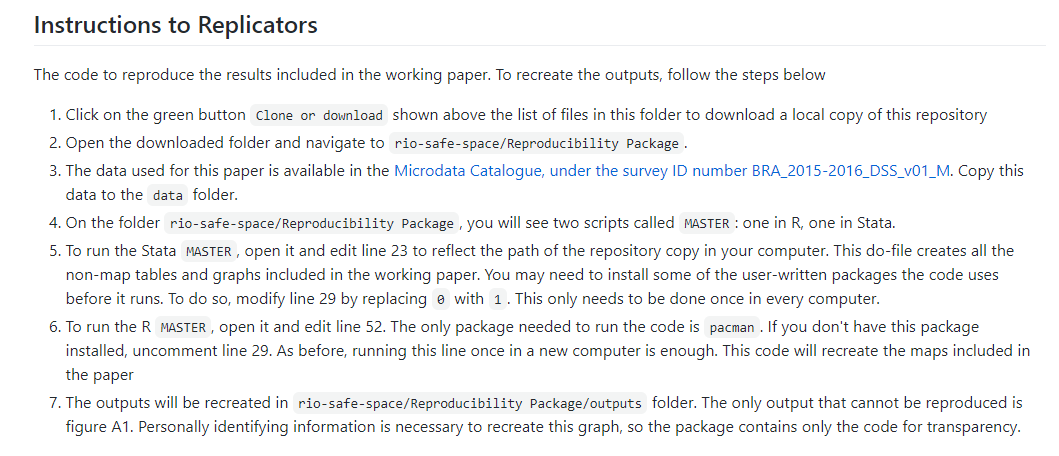
\includegraphics{examples/rep-package.png}

\begin{quote}
The Demand for Safe Space GitHub repository can be viewed at : \url{https://github.com/worldbank/rio-safe-space}
\end{quote}

\begin{quote}
The Microdata Catalog entry for the study is available at \url{https://microdata.worldbank.org/index.php/catalog/3745}
\end{quote}
\end{ex}

\hypertarget{looking-ahead-1}{%
\section*{Looking ahead}\label{looking-ahead-1}}
\addcontentsline{toc}{section}{Looking ahead}

With the ongoing rise of empirical research and increased public scrutiny of scientific evidence,
making analysis code and data available
is necessary but not sufficient to guarantee that findings will be credible.
Even if your methods are highly precise,
your evidence is only as good as your data --
and there are plenty of mistakes that can be made between
establishing a design and generating final results that would compromise its conclusions.
That is why transparency is key for research credibility.
It allows other researchers, and research consumers,
to verify the steps to a conclusion by themselves,
and decide whether their standards for accepting a finding as evidence are met.
Every investment you make in documentation and transparency up front
protects your project down the line, particularly as these standards continue to tighten.
With these principles in mind,
the approach we take to the development, structure,
and documentation of data work
provides a system to implementing these ideas in everyday work.
In the next chapter, we will discuss the workspace you need
in order to work reproducibly in an efficient, organized, and secure manner.

\hypertarget{collaboration}{%
\chapter{Setting the stage for effective and efficient collaboration}\label{collaboration}}

In order to do effective data work in a team environment,
you need to structure your workflow in advance.
Preparation for collaborative data work begins long before you acquire any data,
and involves planning both software tools and collaboration platforms for your team.
This means knowing what types of data you'll acquire,
whether the data will require special handling due to size or privacy considerations,
which datasets and outputs you will need at the end of the process,
and how all data files and versions will stay organized throughout.
It's important to plan data workflows in advance because
changing software or protocols halfway through a project is costly and time-consuming.
Seemingly small decisions such as file-sharing services, folder structures,
and filenames can be extremely painful to alter down the line in any project.

This chapter will guide you in setting up an effective environment for collaborative data work,
structuring your data work to be well-organized and clearly documented,
and setting up processes to handle confidential data securely.
The first section outlines how to set up your working environment
to effectively collaborate on technical tasks with others,
and how to document tasks and decisions.
The second section discusses how to organize your code and data so that others
will be able to understand and interact with it easily.
The third section provides guidelines for ensuring
privacy and security when working with confidential data.

\begin{summary}
\hypertarget{summary-setting-the-stage-for-effective-and-efficient-collaboration-summary}{%
\subsection*{Summary: Setting the stage for effective and efficient collaboration Summary}\label{summary-setting-the-stage-for-effective-and-efficient-collaboration-summary}}
\addcontentsline{toc}{subsection}{Summary: Setting the stage for effective and efficient collaboration Summary}

The technical environment for your data work needs to be established at the start of a research project. Agreeing with the team on software choices, standard code and data structure, and clear data security protocols will prepare you to successfully, safely, and efficiently implement technical tasks throughout the project lifecycle. Consider:

\textbf{1. Technical collaboration environment.} No matter the hardware and software your team plans to use, you should ensure now that it is standardized or interoperable across the team. This includes:

\begin{itemize}
\tightlist
\item
  Secure all \emph{physical computing hardware} through encryption and password-protection. If specialized or more powerful hardware is required, initiate access requests, purchase orders, or other processes now
\item
  Agree on tools for \emph{collaboration} and documentation, such that key conversations and decisions are archived and organized outside of instant-message and email conversation
\item
  Decide the \emph{programming languages and environments} the team will use. Take time to set up a comfortable and modern digital work environment
\end{itemize}

\textbf{2. Organization of code and data}. The team should agree on where and how code files and databases will be stored, down to the level of the folder structure. This involves setting up:

\begin{itemize}
\tightlist
\item
  A standardized and scalable \emph{folder structure} so all documents have an unambiguous location, and the location and naming of files describes their purpose and function and is intuitive to all team members
\item
  A \emph{backup and version control system} appropriate for each file type, to ensure information cannot be lost and that all team members understand how to interoperate and collaborate
\item
  \emph{Master script files} that will structure and execute the code base of the
\end{itemize}

\textbf{3. Information security measures and ethical frameworks}. These include:

\begin{itemize}
\tightlist
\item
  Formally \emph{request and obtain approval} from legal entities governing research in all relevant jurisdictions
\item
  Understand \emph{how to respect the rights and dignity of research subjects} and plan for how to establish \emph{informed consent} from individuals or groups participating in the research
\item
  Adopt standardized \emph{digital security practices} including proper encryption of all confidential information, at rest and in transit, both among your team and with external partners
\end{itemize}

\hypertarget{takeaways-1}{%
\subsubsection*{Takeaways}\label{takeaways-1}}
\addcontentsline{toc}{subsubsection}{Takeaways}

\textbf{TTLs/PIs will:}

\begin{itemize}
\tightlist
\item
  Support the acquisition and maintenance of required computing hardware and software, liaising with procurement, information security and information technology teams as necessary
\item
  Make final decisions regarding code languages and environments
\item
  Discuss and agree upon an appropriate project-wide digital organization strategy\\
\item
  Institute and communicate best practices in accordance with legal, ethical, and security obligations
\end{itemize}

\textbf{RAs will:}

\begin{itemize}
\tightlist
\item
  Communicate technical needs clearly with TTLs/PIs and relevant service providers
\item
  Consistently implement digital organization strategy and flag issues with task management, documentation, or materials storage if they arise
\item
  Support project compliance with ethical, legal, and security obligations and flag concerns to TTLs/PIs
\end{itemize}

\hypertarget{key-resources-1}{%
\subsubsection*{Key Resources}\label{key-resources-1}}
\addcontentsline{toc}{subsubsection}{Key Resources}

\begin{itemize}
\tightlist
\item
  DIME Research Ethics Standards: Pillar 1 of the DIME Research Standards \url{https://github.com/worldbank/dime-standards}
\item
  DIME GitHub Resources: \url{https://github.com/worldbank/dime-github-trainings}\\
\item
  DIME Data Security Standards: Pillar 4 of the DIME Research Standards \url{https://github.com/worldbank/dime-standards}
\item
  DIME Data Publication Standards: Pillar 5 of the DIME Research Standards \url{https://github.com/worldbank/dime-standards}
\end{itemize}
\end{summary}

\hypertarget{preparing-a-collaborative-work-environment}{%
\section*{Preparing a collaborative work environment}\label{preparing-a-collaborative-work-environment}}
\addcontentsline{toc}{section}{Preparing a collaborative work environment}

This section introduces core concepts and tools
for organizing data work in an efficient, collaborative and reproducible manner.
Some of these skills may seem elementary,
but thinking about simple things from a workflow perspective
can help you make marginal improvements every day you work;
those add up to substantial gains over the course of multiple years and projects.
Together, these processes form a collaborative workflow
that will greatly accelerate your team's ability to get tasks done
on all your projects.

Teams often develop workflows in an ad hoc fashion,
solving new challenges as they arise.
Adaptation is good, of course.
But it is important to recognize
that there are a number of tasks that exist in common for every project,
and it is more efficient to agree on the corresponding workflows in advance.
For example, every project requires
research documentation, organized file naming, directory organization,
coding standards, version control, and code review.
These tasks are common to almost every project,
and their solutions translate well between projects.
Therefore, there are large efficiency gains to
thinking in advance about the best way to do these tasks,
instead of throwing together a solution when the task arises.
This section outlines the main points to discuss within the team,
and suggests best practice solutions for these tasks.

\begin{ex}
\hypertarget{demand-for-safe-spaces-case-study-preparing-a-collaborative-work-environment}{%
\subsection*{Demand for Safe Spaces Case Study: Preparing a Collaborative Work Environment}\label{demand-for-safe-spaces-case-study-preparing-a-collaborative-work-environment}}
\addcontentsline{toc}{subsection}{Demand for Safe Spaces Case Study: Preparing a Collaborative Work Environment}

Here are a few highlights of how the \textbf{Demand for Safe Spaces} team chose to organize their work environment for effective collaboration:

\begin{itemize}
\tightlist
\item
  The data work for the project was done through a private GitHub repository housed in the World Bank organization account.
\item
  GitHub issues were used to document research decisions and to provide feedback. Even the PIs for the study, who did not directly participate in coding, used Github issues to review code and outputs and to create a record of broader discussions.
\item
  Stata was adopted as the primary software for data analysis, as that is the software all team members had in common at the start of the project. At a later stage of the project, R code was developed specifically to create maps. The R portion of the code was developed independently, as it used different datasets and created separate outputs. The team used two separate master scripts, one for the Stata code base and one for the R code.\\
\item
  The team members shared a synchronized folder (using Dropbox), which included the de-identified data and project documentation such as survey instruments and enumerator training manuals.
\end{itemize}
\end{ex}

\hypertarget{setting-up-your-computer}{%
\subsection*{Setting up your computer}\label{setting-up-your-computer}}
\addcontentsline{toc}{subsection}{Setting up your computer}

First things first:
almost all your data work will be done on your computer,
so make sure it's set up for success.
The operating system should be fully updated,
it should be in good working order,
and you should have a \textbf{password-protected} login.\index{password protection}
However, password-protection is not sufficient
if your computer stores data that is not public.
You would need to use encryption for sufficient protection,
which will be covered later in this chapter.
Make sure your computer is backed up to prevent information loss.\index{data backup}
Follow the \textbf{3-2-1 rule}: maintain 3 copies of all original or irreplaceable data,
on at least 2 different hardware devices you have access to,
with 1 offsite storage method.\footnote{Read more details about back up strategies
  and other aspects of data storage on the DIME Wiki:
  \url{https://dimewiki.worldbank.org/Data_Storage}.}
Chapter \ref{acquistion} provides a protocol for implementing this.

Ensure you know how to get the \textbf{absolute file path} for any given file.\index{absolute file paths}
On MacOS this will be something like ``\texttt{/users/username/git/project/...}''
and ``\texttt{C:/users/username/git/project/...}'' on Windows.
Absolute file paths will be an obstacle to collaboration
unless they are \textbf{dynamic absolute file paths}.
In a dynamic absolute file path the relative project path,
``\texttt{/git/project/...}'' in the examples above, is added
to the user-specific root path for each user,
``\texttt{/users/username}'' or ``\texttt{C:/users/username}'' in the examples above,
generating an absolute file path unique to each user.
Master scripts introduced later in this chapter will show
how this can be seamlessly implemented.
Dynamic absolute file paths, starting from the file system root,
is the best way to ensure that files are read and written correctly
when multiple users work on the same project
across many different platforms, operative systems and devices.
There are contexts, for example some cloud environments,
where relative file paths must be used,
but in all other contexts we recommend you
to always use dynamic absolute file paths.

Use forward slashes (\texttt{/}) in file paths for folders,
and whenever possible use only the 26 English characters, numbers,
dashes (\texttt{-}), and underscores (\texttt{\_}) in folder names and filenames.\footnote{More naming conventions and links to more resources
  can be found on the DIME Wiki:
  \url{https://dimewiki.worldbank.org/Naming_Conventions}.}\index{filenames}
For emphasis: \emph{always} use forward slashes (\texttt{/})
in file paths in code, just like in internet addresses.
Do this even if you are using a Windows machine where
both forward and backward slashes are allowed,
as your code will otherwise break
if anyone tries to run it on a Mac or Linux machine.
Making the structure of your directories a core part of your workflow is very important,
since otherwise you will not be able to reliably transfer the instructions
for replicating or carrying out your analytical work.

When you are working with others, you will most likely be using
some kind of \textbf{file sharing} software.
\index{file sharing}\index{collaboration tools}
The exact services you use will depend on your tasks,
but in general, there are several approaches to file sharing,
and the three discussed here are the most common.
\textbf{File syncing} is the most familiar method,
and is implemented by software like OneDrive, Dropbox, or Box.
Sync forces everyone to have the same version of every file at the same time,
which makes simultaneous editing difficult but other tasks easier.
\textbf{Distributed version control} is another method,
commonly implemented through systems like GitHub, GitLab, and Bitbucket
that interact with Git.\footnote{\textbf{Git:} A distributed version control system for collaborating on and tracking changes to code as it is written.}
\index{version control}
Distributed version control allows everyone
to access different versions of files at the same time.
It is only optimized for specific types of files
(for example, any type of code files).
Finally, \textbf{server storage} is the least-common method,
because there is only one version of the materials,
and simultaneous access must be carefully regulated.
\index{server storage}
Server storage ensures that everyone has access
to exactly the same files and environment, and it also enables
high-powered computing processes for large and complex data.

All three file sharing methods are used for collaborative workflows,
and you should review the types of data work
that you will be doing, and plan which types of files
will live in which types of sharing services.
It is important to note that they are, in general, not interoperable,
meaning you should not have version-controlled files inside a syncing service,
or vice versa, without setting up complex workarounds,
and you cannot shift files between them without losing historical information.
Therefore, choosing the correct sharing service for each of your team's needs at the outset is essential.
At DIME we typically use file syncing for all project administrative files and data,
version control in Git for code,
and server storage for backup and/or large scale computations when needed.

\hypertarget{establishing-effective-documentation-practices}{%
\subsection*{Establishing effective documentation practices}\label{establishing-effective-documentation-practices}}
\addcontentsline{toc}{subsection}{Establishing effective documentation practices}

Once your technical and sharing workspace is set up,
you need to decide how you are going to communicate with your team.
The first habit that many teams need to break
is using instant communication for management and documentation.
Email is, simply put, not a system. It is not a system for anything.
Neither is instant messaging apps like WhatsApp.\index{email}\index{instant messaging}
Instant messaging tools are developed for communicating ``now'' and that is what they do well.\index{instant messaging}
They are not structured to manage group membership or to present the same information
across a group of people, or to remind you when old information becomes relevant.
They are not structured to allow people to collaborate over a long time or to review old discussions.
It is therefore easy to miss or lose communications from the past when they have relevance in the present.
Everything with future relevance that is communicated over email or any other instant medium
-- such as, for example, decisions about research design --
should immediately be recorded in a system that is designed to keep permanent records.
We call these systems collaboration tools, and there are several that are very useful.

Good collaboration tools are workflow-oriented systems
that allow the team to create and assign tasks,
carry out discussions related to single tasks,
track task progress across time, and quickly see the overall project status.\index{task management}
They are web-based so that everyone on your team can access them simultaneously
and have ongoing discussions about tasks and processes.
Such systems link communications to specific tasks so that
related decisions are permanently recorded
and easy to find in the future when questions about that task come up.
Choosing the right tool for your team's needs is essential to designing an effective workflow.
What is important is that your team chooses a system and commits to using it,
so that decisions, discussions, and tasks are easily reviewable long after they are completed.

Some popular and free collaboration tools that meet these criteria are
GitHub and Dropbox Paper.
Any specific list of software will quickly be outdated;
we mention these as examples that have worked for our team.
Different collaboration tools can be used different types of tasks.
Our team, for example, uses GitHub for code-related tasks,
and Dropbox Paper for more managerial tasks.
GitHub creates incentives for writing down why changes were made
in response to specific discussions
as they are completed, creating naturally documented code.
It is useful also because tasks in GitHub Issues can clearly be tied to file versions.
On the other hand, Dropbox Paper provides a clean interface with task notifications,
assignments, and deadlines,
and is very intuitive for people with non-technical backgrounds.
Therefore, it is a useful tool for managing non-code-related tasks.

\hypertarget{setting-up-your-code-environment}{%
\subsection*{Setting up your code environment}\label{setting-up-your-code-environment}}
\addcontentsline{toc}{subsection}{Setting up your code environment}

Taking time early in your project to choose a programming language to work in and
setting up a productive code environment for that language
will make your work significantly easier.
\index{code environment}
Setting up a productive code environment means to
make sure that the programming language and all other software your code requires
will run smoothly on all the hardware you need it to run on.
It also means that you have a productive way of interacting with code,
and that the code has a seamless method to access your data.

It is difficult and costly to switch programming languages halfway through a project,
so think ahead about the various software your team will use.
Take into account the technical abilities of team members,
what type of internet access the software will need,
the type of data you will need to access,
and the level of security required.
Big datasets require additional infrastructure and may overburden
the tools commonly used for small datasets.
Also consider the cost of licenses, the time to learn new tools,
and the stability of the tools.
There are few strictly right or wrong choices for software,
but what is important is that you plan in advance
and understand how the chosen tools will interact with your workflows.

One option is to hold your code environment constant
over the lifecycle of a single project.
While this means you will inevitably have different projects
with different code environments, each successive project will be better than the last,
and you will avoid the costly process of migrating an ongoing project
into a new code environment.
Code environments should be documented as precisely as possible.
The specific version number of the programming languages and the individual packages you use
should be referenced or maintained so that they can be reproduced going forward,
even if different releases contain changes that would break your code
or change your results.
\index{software versions}
DIME Analytics developed the command \texttt{ieboilstart} in the \texttt{ietoolkit} package
to support version and settings stability in Stata.\footnote{Read more about how to install and use \texttt{ieboilstart}
  and how it can help you harmonize settings across users
  as much as possible in Stata on the DIME Wiki:
  \url{https://dimewiki.worldbank.org/ieboilstart}.}
If your project requires more than one programming language,
for example if you analyze your data in one language but visualize your results in another,
then make sure to make an as clear division between the two as possible.
This means that you first complete all tasks done in one language,
before the completing the rest of the tasks in the other language.
Frequently swapping back and forth between languages is a reproducibility nightmare.

Next, think about how and where you write and execute code.
This book is intended to be agnostic to the size or origin of your data,
but we are going to broadly assume that you are using
one of the two most popular statistical software packages: R or Stata.
(If you are using another language, like Python,
many of the same principles apply but the specifics will be different.)
Most of your code work will be done in a code editor.
If you are working in R, \textbf{RStudio} is the typical choice.\footnote{\url{https://www.rstudio.com}}
For Stata, the built-in do-file editor is the most widely adopted code editor.
You might also consider using an external editor for your R or Stata code.\footnote{More details on the benefits of external code editors and
  links to popular code editors can be found on the DIME Wiki:
  \url{https://dimewiki.worldbank.org/Code_Editors}.}
These editors offer great accessibility and quality features.
For example, they can access an entire directory -- rather than a single file --
which gives you directory-level views and file management actions,
such as folder management, Git integration,
and simultaneous work with other types of files, without leaving the editor.
Using an external editor can also be preferable since your editor will not crash
if the execution of your code causes your statistical software to crash.
Finally, you can often use the same editor for all programming languages you use,
so any customization you do in your code editor of choice
will improve your productivity across all your coding work.

\hypertarget{organizing-code-and-data-for-replicable-research}{%
\section*{Organizing code and data for replicable research}\label{organizing-code-and-data-for-replicable-research}}
\addcontentsline{toc}{section}{Organizing code and data for replicable research}

We assume you are going to do your analytical work through code,
and that you want all your processes to be documented and replicable.
Though it is possible to interact with some statistical software
through the user interface without writing any code,
we strongly advise against it.
Writing code creates a record of every task you performed.
It also prevents direct interaction with the data files that could lead to non-reproducible steps.
You may do some exploratory tasks by point-and-click or typing directly into the console,
but anything that is included in a research output
must be coded in an organized fashion so that you can release
the exact code that produces your final results --
up to and including individual statistics in text.
Still, organizing code and data into files and folders is not a trivial task.
What is intuitive to one person rarely comes naturally to another,
and searching for files and folders is everybody's least favorite task.
As often as not, you come up with the wrong one,
and then it becomes very easy to create problems that require complex resolutions later.
This section provides basic tips on managing the folder
that stores your project's data work.

Maintaining an organized file structure for data work is the best way
to ensure that you, your teammates, and others
are able to easily edit and replicate your work in the future.
It also ensures that automated processes from code and scripting tools
are able to interact well with your work,
whether they are yours or those of others.
File organization makes data work easier as well as more transparent,
and facilitates integration with tools like version control systems
that aim to cut down on the amount of repeated tasks you have to perform.
It is worth thinking in advance about how to store, name, and organize
the different types of files you will be working with,
so that there is no confusion down the line
and everyone has the same expectations.

\hypertarget{organizing-files-and-folders}{%
\subsection*{Organizing files and folders}\label{organizing-files-and-folders}}
\addcontentsline{toc}{subsection}{Organizing files and folders}

Once you start a research project,
the number of scripts, datasets, and outputs
that you have to manage will grow very quickly.
This can get out of hand just as quickly,
so it's important to organize your data work
and follow best practices from the beginning.
You should agree with your team on a specific directory structure,
and set it up at the beginning of the project.
You should also agree on a file naming convention.
This will help you to easily find project files and
ensure that all team members can easily run the same code.

To support consistent folder organization at DIME,
DIME Analytics created \texttt{iefolder}
as a part of our \texttt{ietoolkit} package.\footnote{Read more about how to install and use \texttt{iefolder},
  as well as find links to resources explaining
  the best practices this command build upon on the DIME Wiki:
  \url{https://dimewiki.worldbank.org/iefolder}.}\index{iefolder}\index{ietoolkit}
This Stata command sets up a pre-standardized folder structure
for what we call the \texttt{DataWork} folder.\footnote{More details on DIME's suggested data work folder structure
  and explanations of the best practices it is based on
  can be found on the DIME Wiki:
  \url{https://dimewiki.worldbank.org/DataWork_Folder}.}
The \texttt{DataWork} folder includes folders for all the steps of a typical project.
\index{DataWork folder}
Since each project will always have unique needs,
we have tried to make the structure easy to adapt.
Having a universally standardized folder structure
across the entire portfolio of projects
means that everyone can easily move between projects
without having to reorient on file and folder organization.

If you do not already have a standard file structure across projects,
\texttt{iefolder} is an easy template to start from.
The command creates a \texttt{DataWork} folder at the project level,
and within that folder, creates standardized directory structures
for each data source or survey round.
Within each subdirectory, \texttt{iefolder} creates folders for raw encrypted data,
raw deidentified data, cleaned data, final data, outputs, and documentation.
It creates a parallel folder structure for the code files
that move the data through this progression,
and for the final analytical outputs.
The \texttt{ietoolkit} package also includes the \texttt{iegitaddmd} command,
which can place \texttt{README.md} placeholder files in your folders so that
your folder structure can be shared using Git.\footnote{Git only tracks files, so empty folders
  -- which most folders are in the beginning of a project --
  are ignored if placeholder files are not used,
  leading to only parts of the folder structure being shared across the team.
  Read more about how to install and use \texttt{iegitaddmd}
  and how it can help you track empty folder in Git on the DIME Wiki:
  \url{https://dimewiki.worldbank.org/Iegitaddmd}.}
Since these placeholder files are written in a plaintext language called \textbf{Markdown},
they also provide an easy way to document the contents of every folder in the structure.
\index{Markdown}

The \texttt{DataWork} folder may be created either inside
an existing project folder, or it may be created as a separate root folder.
We advise keeping project management materials
(such as contracts, terms of reference, briefs and other administrative or management work)
separate from the \texttt{DataWork} folder structure.
It is useful to maintain project management materials in a sync system like Dropbox,
whereas the code folder should be maintained in a version-control system like Git.
However, a version-controlled folder should \emph{never}
be stored in a synced folder that is shared with other people.
Combining these two types of collaboration tools
almost always creates undesired functionalities.

\begin{ex}
\hypertarget{demand-for-safe-spaces-case-study-organizing-files-and-folders}{%
\subsection*{Demand for Safe Spaces Case Study: Organizing Files and Folders}\label{demand-for-safe-spaces-case-study-organizing-files-and-folders}}
\addcontentsline{toc}{subsection}{Demand for Safe Spaces Case Study: Organizing Files and Folders}

The diagram below illustrates the folder structure for the \emph{Demand for Safe Spaces} data work. Note that this project started before the \texttt{iefolder} structured was created, and so differs from the current guidelines. Changing folder organization midway through a project is never recommended. The key feature of folder organization is planning ahead and agreeing with the whole team on the best structure to follow.

The root folder for the study's data work included two master scripts (one for Stata and one R, that can be run independently), a readme, and 4 subfolders: data, code, documentation and outputs. The folder structure was identical in GitHub and DropBox, but the files present in each of them differed. All code, raw outputs (such as TeX table fragments and PNG images) and plain text documentation were stored in GitHub. All the datasets, PDF outputs and documentation in Word and Excel were stored in DropBox. When data processing was completed, binary files in the Documentation folder that were accessed by the code, such as \texttt{iecodebook} and \texttt{ieduplicates} spreadsheets, were moved to GitHub to ensure completeness of the repository.

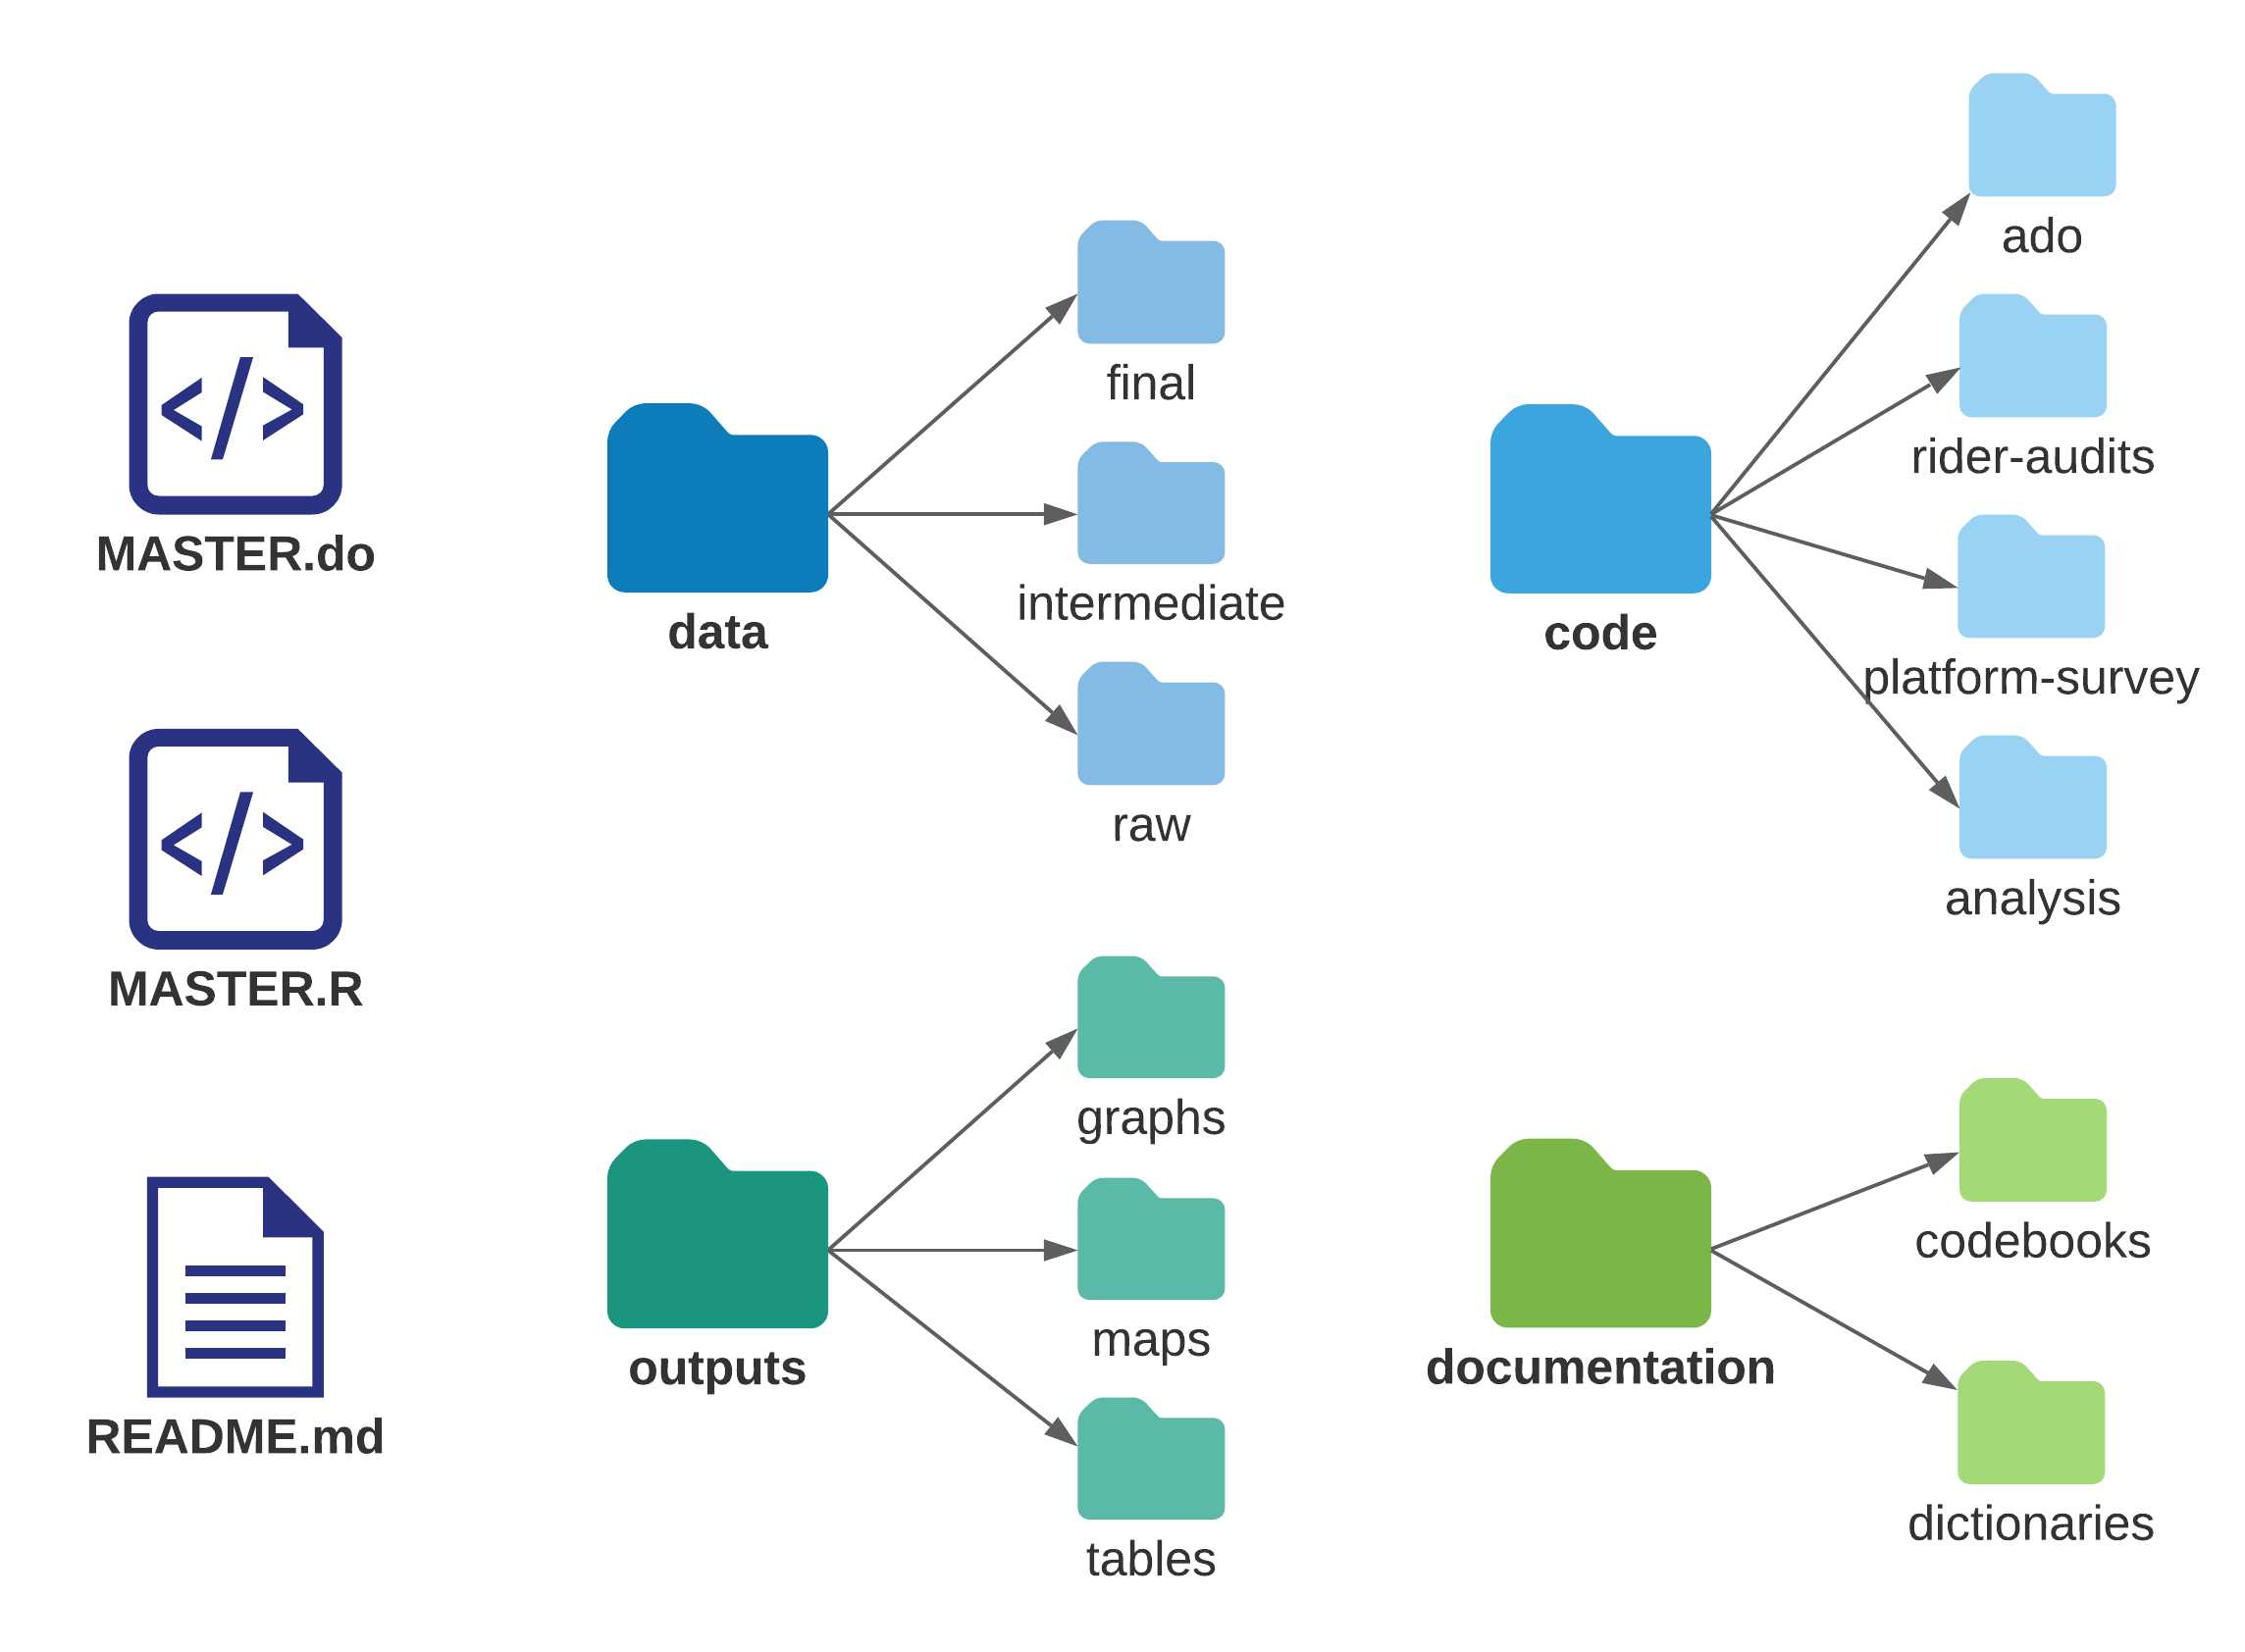
\includegraphics{examples/folder-structure.png}
\end{ex}

\hypertarget{establishing-common-file-formats}{%
\subsection*{Establishing common file formats}\label{establishing-common-file-formats}}
\addcontentsline{toc}{subsection}{Establishing common file formats}

Each task in the research workflow has specific inputs and outputs
which feed into one another.
It is common, particularly when different tasks are performed by different people inside a team,
for incompatibilities to be created.
For example, if the Principal Investigators are writing a paper using LaTeX,
exporting tables from statistical software into a \texttt{.csv} format will break the workflow.
Therefore, it's important to agree with your team on what tools will be used for what tasks,
and where inputs and outputs will be stored, before you start creating them.
Take into account ease of use for different team members,
and keep in mind that learning how to use a new tool may require some time investment upfront that will be paid off as your project advances.

Knowing how code outputs will be used will help you decide the best format to export them.
You can typically use the same software to save figures into various formats,
such as \texttt{.eps\},}.png\texttt{,}.pdf\texttt{or}.jpg`.
However, the decision between using Office Suite software
such as Word and PowerPoint versus LaTeX and other plain text formats
may influence how you write your code,
as this choice often implicates in the use of a particular format.
This decision will also affect the version control systems that your team can use.

\hypertarget{using-version-control}{%
\subsection*{Using version control}\label{using-version-control}}
\addcontentsline{toc}{subsection}{Using version control}

We recommend using a \textbf{version control system} to
maintain control of file history and functionality.
A good version control system tracks who edited each file and when,
allows you to revert to previous versions,
and provides a protocol for ensuring that conflicting versions are avoided.
This is important, for example, for your team
to be able to find the version of a presentation that you delivered to a donor,
or to understand why the significance level of your estimates has changed.
Everyone who has ever encountered a file named something like \texttt{final\_report\_v5\_LJK\_KLE\_jun15.docx}
can appreciate how useful such a system can be.

Most syncing services offer some kind of rudimentary version control;
these are usually enough to manage changes to binary files (such as office documents)
without needing to rely on dreaded filename-based versioning conventions.
For code files, however, a more detailed version control system is usually desirable.
We recommend using Git for version-control of all data work.
Git documents changes to all \textbf{plaintext} files.
Plaintext files include all code files, most raw outputs,
and written outputs that use code languages,
such as LaTeX files and many dynamic documents.\index{LaTeX}\index{dynamic documents}
Git tracks all the changes you make to each plaintext file,
and allows you to go back to previous versions without losing the information on changes made.
It also makes it possible to work on multiple parallel versions of a file,
so you don't risk breaking code for other team members as you try something new.

\hypertarget{writing-code-that-others-can-read}{%
\subsection*{Writing code that others can read}\label{writing-code-that-others-can-read}}
\addcontentsline{toc}{subsection}{Writing code that others can read}

Good code is written in a way that is easily understood and run by others.
Below we discuss a few crucial steps to code organization.
They all come from the principle that code is an output by itself,
not just a means to an end,
and should be written thinking of how easy it will be for someone to read it later.
At the end of this section, we include a template for a master script do-file in Stata,
to provide a concrete example of the required elements and structure.
Throughout this section, we refer to lines of this example do-file
to give concrete examples of the required code elements, organization and structure.

To be readable, code must be well-documented.
Start by adding a code header to every file.\index{code header}
A code header is a long \textbf{comment}\footnote{\textbf{Comments:} Code components that have no function to the computer,
  but describe in plain language for humans to read
  what the code is supposed to do.}\index{code comments}
that details the functionality of the entire script;
refer to lines 5-10 in the example do-file.
This should include simple things such as
the purpose of the script and the name of the person who wrote it.
If you are using a version control software,
the last time a modification was made and the person who made it will be recorded by that software.
Otherwise, you should include it in the header.
You should always track the inputs and outputs of the script,
as well as the uniquely identifying variable;
refer to lines 52-54 in the example do-file.
When you are trying to track down which code creates which dataset, this will be very helpful.
While there are other ways to document decisions related to creating code,
the information that is relevant to understand the code should always be written in the code file.

Two types of comments should be included in the script itself.
The first type of comment describes \emph{what} is being done.
This might be easy to understand from the code itself
if you know the language well enough and the code is clear,
but often it is still a great deal of work to reverse-engineer the code's intent.
Describing the task in plain English (or whichever language you use to communicate with your team)
will make it easier for everyone to read and understand the code's purpose.
It can also help you organize your own work and ensure you are following logical steps.
The second type of comment explains \emph{why} the code is performing a task in a particular way.
As you are writing code, you are making a series of decisions that
(hopefully) make perfect sense to you at the time.
These are often highly specialized and may exploit a functionality
that is not obvious or has not been seen by others before.
Well-commented code is in itself a great way to document your data work
which someone can follow to understand anything from
data cleaning decisions that make the published data differ from the original data
to decisions on how indicators are constructed.
Even you will probably not remember the exact choices that were made in a couple of weeks.
Therefore, you must document your precise processes in your code.

Code files should be stored in an easy-to-find location and named in a meaningful way.
\index{code organization}
Breaking your code into independently readable ``chunks'' is good practice for code organization.\index{code chunks}
You should write each functional element as a chunk that can run completely on its own.
This ensures that each code component is independent;
it does not rely on a complex program state
created by other code chunks that are not obvious from the immediate context.
One way to do this is by creating sections in your script to identify where a specific task is completed.
For example, if you want to find the line in your code where the directory is set,
you can go straight to \texttt{PART\ 2:\ Prepare\ folder\ paths\ and\ define\ programs},
instead of reading line by line through the entire code.

RStudio makes it very easy to create sections,
and it compiles them into an interactive script index for you.
In Stata, you can use comments to create section headers
(see line 27 of the example do-file),
though they're just there to make the reading easier and don't have functionality.
Since an index is not automated,
create this manually in the code header by copying and pasting section titles
(see lines 8-10 in the example do-file).
You can then add and navigate through them using the \texttt{find} functionality.
Since Stata code is harder to navigate, as you will need to scroll through the document,
it's particularly important to avoid writing very long scripts.
Therefore, in Stata at least, we recommend breaking code tasks down
into separate do-files, since there is no limit on how many you can have,
how detailed their names can be, and no advantage to writing longer files.
One reasonable rule of thumb is to not write do-files that have more than 200 lines.
This is an arbitrary limit, just like the common practice of limiting code lines to 80 characters:
it seems to be ``enough but not too much'' for most purposes.

\begin{ex}
\hypertarget{demand-for-safe-spaces-case-study-writing-code-that-others-can-read}{%
\subsection*{Demand for Safe Spaces Case Study: Writing Code That Others Can Read}\label{demand-for-safe-spaces-case-study-writing-code-that-others-can-read}}
\addcontentsline{toc}{subsection}{Demand for Safe Spaces Case Study: Writing Code That Others Can Read}

To ensure that all team members were able to easily read and understand data work, \emph{Demand for Safe Spaces} code files were extensively commented. Comments typically took the form of ``what -- why'': what is this section of code doing, and why is it necessary. The below snippet from a do-file cleaning one of the raw data files illustrates the use of comments:

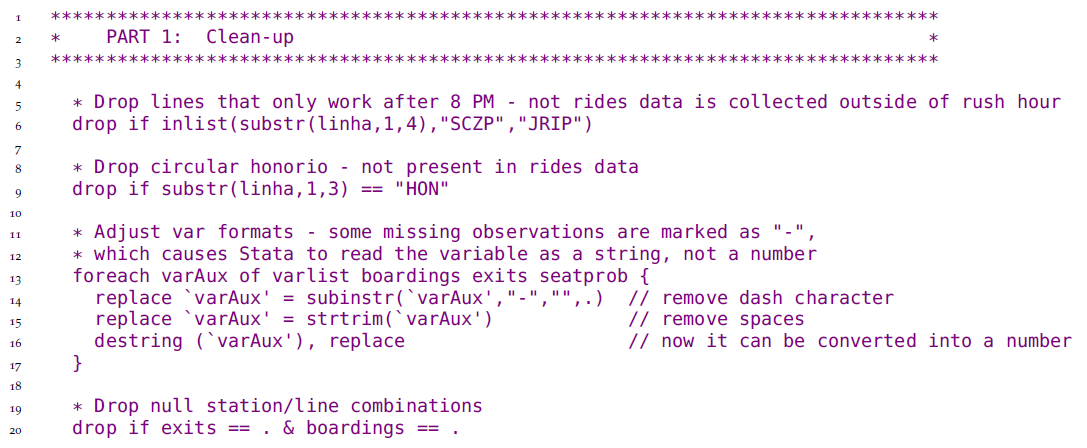
\includegraphics{examples/ch2-writing-code-that-others-can-read.png}

\begin{quote}
The full code file is available at \url{https://git.io/Jtgev}
\end{quote}
\end{ex}

\hypertarget{writing-code-that-others-can-run}{%
\subsection*{Writing code that others can run}\label{writing-code-that-others-can-run}}
\addcontentsline{toc}{subsection}{Writing code that others can run}

To bring all these smaller code files together, you must maintain a master script.\footnote{More details and description of each section of our template master do-file
  can be found on the DIME Wiki:
  \url{https://dimewiki.worldbank.org/Master_Do-files}.}
\index{master script}
A master script is the map of all your project's data work
which serves as a table of contents for the instructions that you code.
Anyone should be able to follow and reproduce all your work from
raw data to all outputs by simply running this single script.
By follow, we mean someone external to the project who has the master script and all the input data can
(i) run all the code and recreate all outputs,
(ii) have a general understanding of what is being done at every step, and
(iii) see how codes and outputs are related.
The master script is also where all the settings are established,
such as versions, folder paths, functions, and constants used throughout the project.

\begin{Shaded}
\begin{Highlighting}[numbers=left,,]
\CommentTok{/*******************************************************************************}
\CommentTok{*                           TEMPLATE MASTER DO-FILE                            *}
\CommentTok{********************************************************************************}
\CommentTok{*                                                                              *}
\CommentTok{*   PURPOSE:     Reproduce all data work, map inputs and outputs,              *}
\CommentTok{*                facilitate collaboration                                      *}
\CommentTok{*                                                                              *}
\CommentTok{*   OUTLINE:     PART 1:  Set standard settings and install packages           *}
\CommentTok{*                PART 2:  Prepare folder paths and define programs             *}
\CommentTok{*                PART 3:  Run do-files                                         *}
\CommentTok{*                                                                              *}
\CommentTok{********************************************************************************}
\CommentTok{  PART 1:  Install user-written packages and harmonize settings}
\CommentTok{********************************************************************************/}

    \KeywordTok{local}\NormalTok{ user_commands ietoolkit iefieldkit }\CommentTok{//Add required user-written commands}
    \KeywordTok{foreach}\NormalTok{ command }\KeywordTok{of} \KeywordTok{local}\NormalTok{ user_commands \{}
\NormalTok{        cap which }\OtherTok{`command'}
        \KeywordTok{if} \DataTypeTok{_rc}\NormalTok{ == 111 }\KeywordTok{ssc}\NormalTok{ install }\OtherTok{`command'}
\NormalTok{    \}}

\NormalTok{    *Harmonize settings across users }\KeywordTok{as}\NormalTok{ much }\KeywordTok{as}\NormalTok{ possible}
\NormalTok{    ieboilstart, v(13.1)}
    \OtherTok{`r(version)'}

\CommentTok{/*******************************************************************************}
\CommentTok{  PART 2:  Prepare folder paths and define programs}
\CommentTok{*******************************************************************************/}

\NormalTok{    * Research Assistant folder paths}
    \KeywordTok{if} \StringTok{"`c(username)'"}\NormalTok{ == }\StringTok{"ResearchAssistant"}\NormalTok{ \{}
        \KeywordTok{global}\NormalTok{ github      }\StringTok{"C:/Users/RA/Documents/GitHub/d4di/DataWork"}
        \KeywordTok{global}\NormalTok{ dropbox     }\StringTok{"C:/Users/RA/Dropbox/d4di/DataWork"}
        \KeywordTok{global}\NormalTok{ encrypted   }\StringTok{"M:/DataWork/EncryptedData"}
\NormalTok{    \}}

\NormalTok{    * Baseline folder globals}
    \KeywordTok{global}\NormalTok{ bl_encrypt       }\StringTok{"$\{encrypted\}/Round Baseline Encrypted"}
    \KeywordTok{global}\NormalTok{ bl_dt            }\StringTok{"$\{dropbox\}/Baseline/DataSets"}
    \KeywordTok{global}\NormalTok{ bl_doc           }\StringTok{"$\{dropbox\}/Baseline/Documentation"}
    \KeywordTok{global}\NormalTok{ bl_do            }\StringTok{"$\{github\}/Baseline/Dofiles"}
    \KeywordTok{global}\NormalTok{ bl_out           }\StringTok{"$\{github\}/Baseline/Output"}

\CommentTok{/*******************************************************************************}
\CommentTok{  PART 3: Run do-files}
\CommentTok{*******************************************************************************/}

\CommentTok{/*------------------------------------------------------------------------------}
\CommentTok{    PART 3.1:  De-identify baseline data}
\CommentTok{    REQUIRES:   $\{bl_encrypt\}/Raw Identified Data/D4DI_baseline_raw_identified.dta}
\CommentTok{    CREATES:    $\{bl_dt\}/Raw Deidentified/D4DI_baseline_raw_deidentified.dta}
\CommentTok{    IDS VAR:    hhid}
\CommentTok{----------------------------------------------------------------------------- */}
\NormalTok{    *Change the 0 to 1 to }\KeywordTok{run}\NormalTok{ the baseline }\KeywordTok{de}\NormalTok{-identification dofile}
    \KeywordTok{if}\NormalTok{ (0) }\KeywordTok{do} \StringTok{"$\{bl_do\}/Cleaning/deidentify.do"}

\CommentTok{/*------------------------------------------------------------------------------}
\CommentTok{    PART 3.2:  Clean baseline data}
\CommentTok{    REQUIRES:   $\{bl_dt\}/Raw Deidentified/D4DI_baseline_raw_deidentified.dta}
\CommentTok{    CREATES:    $\{bl_dt\}/Final/D4DI_baseline_clean.dta}
\CommentTok{                $\{bl_doc\}/Codebook baseline.xlsx}
\CommentTok{    IDS VAR:    hhid}
\CommentTok{----------------------------------------------------------------------------- */}
\NormalTok{    *Change the 0 to 1 to }\KeywordTok{run}\NormalTok{ the baseline cleaning dofile}
    \KeywordTok{if}\NormalTok{ (0) }\KeywordTok{do} \StringTok{"$\{bl_do\}/Cleaning/cleaning.do"}

\CommentTok{/*-----------------------------------------------------------------------------}
\CommentTok{    PART 3.3:  Construct income indicators}
\CommentTok{    REQUIRES:   $\{bl_dt\}/Final/D4DI_baseline_clean.dta}
\CommentTok{    CREATES:    $\{bl_out\}/Raw/D4DI_baseline_income_distribution.png}
\CommentTok{                $\{bl_dt\}/Intermediate/D4DI_baseline_constructed_income.dta}
\CommentTok{    IDS VAR:    hhid}
\CommentTok{----------------------------------------------------------------------------- */}
\NormalTok{    *Change the 0 to 1 to }\KeywordTok{run}\NormalTok{ the baseline }\KeywordTok{variable}\NormalTok{ construction dofile}
    \KeywordTok{if}\NormalTok{ (0) }\KeywordTok{do} \StringTok{"$\{bl_do\}/Construct/construct_income.do"}
\end{Highlighting}
\end{Shaded}

Try to create the habit of running your code from the master script.
Creating ``section switches'' using macros or objects to run only the codes related to a certain task
should always be preferred to manually open different scripts to run them in a certain order
(see the \texttt{if\ (0)} switches in Part 3 of \texttt{stata-master-dofile.do} for one way of how to do this).\index{code section switches}
Furthermore, running all scripts related to a particular task through the master whenever one of them is edited
helps you identify unintended consequences of the changes you made.
Say, for example, that you changed the name of a variable created in one script.
This may break another script that refers to this variable.
But unless you run both of them when the change is made, it may take time for that to happen,
and when it does, it may take time for you to understand what's causing an error.
The same applies to changes in datasets and results.

To link code, data and outputs,
the master script reflects the structure of the \texttt{DataWork} folder in code
through globals (in Stata) or string scalars (in R);
refer to lines 38-43 of the example do-file.
These coding shortcuts can refer to subfolders,
so that those folders can be referenced without repeatedly writing out their absolute file paths.
Because the \texttt{DataWork} folder is shared by the whole team,
its structure is the same in each team member's computer.
The only difference between machines should be
the path to the project root folders, i.e.~the highest-level shared folder.
Depending on your software environment you may have multiple root folders.
In a typical DIME project we have one Git root folder for our code,
one sync software root folder for our de-identified data,
and a third for our encrypted data.
This is reflected in the master script in such a way that
the only change necessary to run the entire code for a new team member
is to change the path to the project root folders
to reflect the file system and username;
refer to lines 30-35 of the example do-file.
The code in \texttt{stata-master-dofile.do} shows how folder structure is reflected in a master do-file.
Because writing and maintaining a master script can be challenging as a project grows,
an important feature of the \texttt{iefolder} is to write sub-master do-files
and add to them whenever new subfolders are created in the \texttt{DataWork} folder.\index{iefolder}

In order to maintain well-documented and organized code,
you should agree with your team on a plan to review code as it is written.
\index{code review}
Reading other people's code is the best way to improve your coding skills.
And having another set of eyes on your code will make you more comfortable with the results you find.
It's normal (and common) to make mistakes as you write your code.
Reading it again to organize and comment it as you prepare it to be reviewed will help you identify them.
Try to have a code review scheduled frequently,
every time you finish writing a piece of code, or complete a small task.
If you wait for a long time to have your code reviewed, and it gets too complex,
preparation and code review will require more time and work,
and that is usually the reason why this step is skipped.
One other important advantage of code review is that
making sure that the code is running properly on other machines,
and that other people can read and understand the code easily,
is the easiest way to be prepared in advance for a smooth project handover
or for release of the code to the general public.

\begin{ex}
\hypertarget{demand-for-safe-spaces-case-study-writing-code-that-others-can-run}{%
\subsection*{Demand for Safe Spaces Case Study: Writing Code That Others Can Run}\label{demand-for-safe-spaces-case-study-writing-code-that-others-can-run}}
\addcontentsline{toc}{subsection}{Demand for Safe Spaces Case Study: Writing Code That Others Can Run}

All code for the \emph{Demand for Safe Spaces} study was organized to run from two master scripts, one Stata Master and one R Master. The master scripts were written such that any team member could run all project code by simply changing the top-level directory. Below is a snippet of the Stata Master:

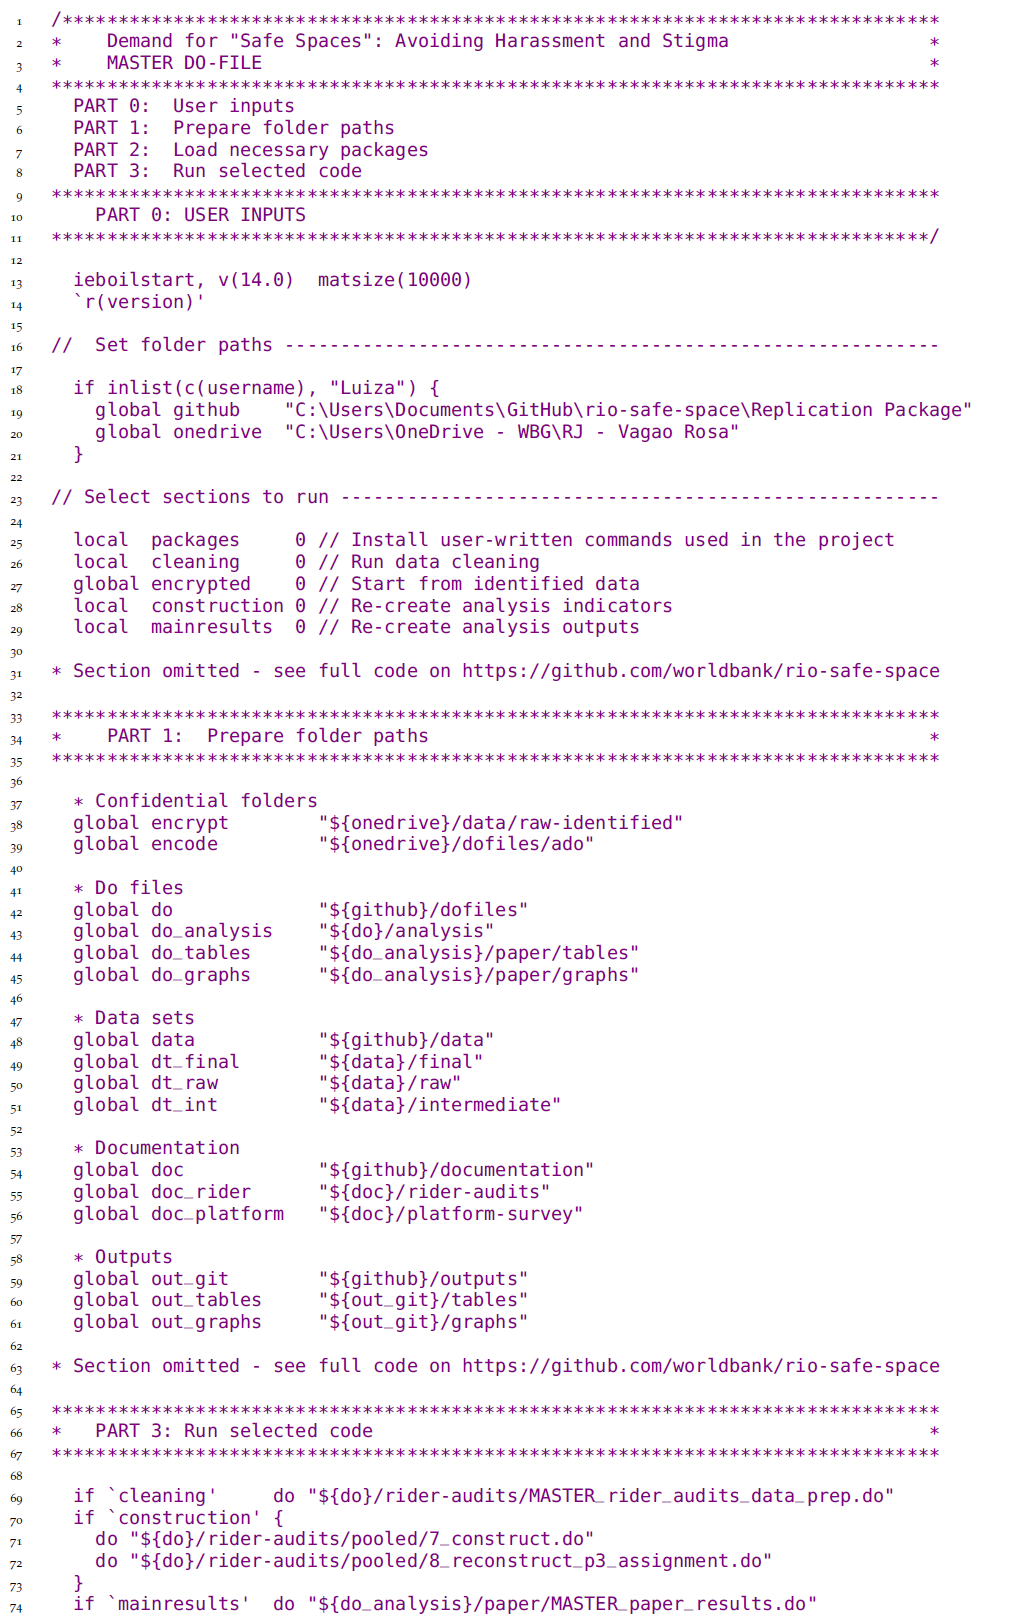
\includegraphics{examples/ch2-writing-code-that-others-can-run.png}

\begin{quote}
The complete Stata master script can be found at \url{https://git.io/JtgeT}, and the R master at \url{https://git.io/JtgeY}.
\end{quote}
\end{ex}

\hypertarget{preparing-to-handle-confidential-data-ethically}{%
\section*{Preparing to handle confidential data ethically}\label{preparing-to-handle-confidential-data-ethically}}
\addcontentsline{toc}{section}{Preparing to handle confidential data ethically}

Anytime you are working with original data in a development research project,
you are almost certainly handling data that include
\textbf{personally-identifying information (PII)}.\index{personally-identifying information (PII)}\footnote{\textbf{Personally-identifying information:} any piece or set of information
  that can be used to identify an individual research subject.
  Read more about what extra consideration
  you must take into account when
  working with PII data on the DIME Wiki:
  \url{https://dimewiki.worldbank.org/Protecting_Human_Research_Subjects}.}
PII is information which can, without any transformation or linkage,
be used to identify individual people, households, firms,
(or other units) in your data.
Some examples of PII variables include names, addresses, and geolocations,
email addresses, phone numbers,
and bank accounts or other financial details.\index{geodata}
If you are working in a context or population that is either small, specific,
or has extensive linkable data sources available to others,
information like someone's age and gender may be sufficient to
disclose their identify, even though those variables would not be considered PII in general.

In a collaborative project,
you will sometimes need to transfer and work with PII information,
and sometimes you will prefer to remove or mask PII
before transferring or working with data.
There is no one-size-fits-all solution to determine what is PII,
research teams have to use careful judgment in each case to avoid statistical disclosure.\footnote{More details on statistical disclosure and
  links to best practices related to data publication,
  can be found on the DIME Wiki:
  \url{https://dimewiki.worldbank.org/Publishing_Data}.}
\index{statistical disclosure}\index{data release}
It is important to keep in mind that data privacy principles apply
not only for the respondent giving you the information
but also for their household members or other individuals who are included in the data.

In all cases where confidential information is involved,
you must make sure that you adhere to several core principles.
These include ethical approval, participant consent,
data security, and participant privacy.\footnote{See Baldwin, Muyengwa, and Mvukiyehe (\protect\hyperlink{ref-baldwin2017reforming}{2017}) for an example.}
If you are a US-based researcher, you will become familiar
with a set of governance standards known as ``The Common Rule.''\footnote{Bierer, Barnes, and Lynch (\protect\hyperlink{ref-bierer2017revised}{2017})}
If you interact with European institutions or persons,
you will also become familiar with the General Data Protection Regulation (GDPR),\footnote{\url{https://gdpr-info.eu}}
a set of regulations governing \textbf{data ownership} and privacy standards.\index{data ownership}
No matter who you are or what exact legal requirements you face,
the core principles and practices you need to consider will always be similar.

\hypertarget{seeking-ethical-approval}{%
\subsection*{Seeking ethical approval}\label{seeking-ethical-approval}}
\addcontentsline{toc}{subsection}{Seeking ethical approval}

Most of the field research done in development involves human subjects.\footnote{Read more about what extra consideration
  you must take into account when
  working with human subjects on the DIME Wiki:
  \url{https://dimewiki.worldbank.org/Protecting_Human_Research_Subjects}}
\index{human subjects}
As a researcher, you are asking people to trust you with personal information about themselves:
where they live, how rich they are, whether they have committed or been victims of crimes,
their names, their national identity numbers, and all sorts of other data.
PII data carries strict expectations about data storage and handling,
and it is the responsibility of the research team to satisfy these expectations.\footnote{More details on research ethics as well as links to tools and
  other resources related can be found on the DIME Wiki:
  \url{https://dimewiki.worldbank.org/Research_Ethics}.
  More details can also be found under Pillar 1 in the DIME Research Standards:
  \url{https://github.com/worldbank/dime-standards}}
Your donor or employer will most likely require you to hold a certification from a respected source.

For almost all such data collection and research activities,
you will be required to complete some form of \textbf{Institutional Review Board (IRB)} process.\footnote{\textbf{Institutional Review Board (IRB):} An institution formally responsible for ensuring that research meets ethical standards.}
\index{institutional review board (IRB)}
Most commonly this consists of a formal application for approval of a specific
protocol for consent, data collection, and data handling.\footnote{More details and best practices for how to submit a project for an IRB approval
  can be found on the DIME Wiki:
  \url{https://dimewiki.worldbank.org/IRB_Approval}.}
Which IRB has authority over your project is not always apparent,
particularly if some institutions do not have their own.
It is customary to obtain an approval from a university IRB
where at least one PI is affiliated,
and if work is being done in an international setting,
approval is often also required
from an appropriate local institution subject to the laws of the country where data originates.

IRB approval should be obtained well before any data is acquired.
IRBs may have infrequent meeting schedules
or require several rounds of review for an application to be approved.
If there are any deviations from an approved plan or expected adjustments,
report these as early as possible so that you can update or revise the protocol.
IRBs have the authority to retroactively deny
the right to use data which was not acquired in accordance with an approved plan.
This is extremely rare, but shows the seriousness of these considerations
since the institution itself may face legal penalties if its IRB
is unable to enforce them. As always, as long as you work in good faith,
you should not have any issues complying with these regulations.

\begin{ex}
\hypertarget{demand-for-safe-spaces-example-seeking-ethical-approval}{%
\subsection*{Demand for Safe Spaces Example -- Seeking Ethical Approval}\label{demand-for-safe-spaces-example-seeking-ethical-approval}}
\addcontentsline{toc}{subsection}{Demand for Safe Spaces Example -- Seeking Ethical Approval}

The Duke University IRB reviewed and approved the protocol for all components of fieldwork for the \emph{Demand for Safe Spaces} study (IRB number D0190). As one of the PIs was at Duke, and the World Bank does not have an IRB, Duke was the relevant institution in this case. The study was registered with the Duke IRB on September 2015. It was amended 4 times to reflect additions to the study design, such as an implicit association test (IAT) and a new survey. The IRB approval was renewed twice, in 2016 and 2017.
Highlights from the study IRB protocols:

\begin{itemize}
\tightlist
\item
  \emph{Voluntary study participation:} The study intervention was done through a smartphone application. Through the app, users were offered payment to complete a set of tasks while using the metro. The tasks involved answering questions at different moments of the trip (before boarding the train, during the ride, after leaving the train). At the start of each task, participants could review what it comprised and the exact payment value, then decide whether to accept the task or not. There was no obligation to complete any task.
\item
  \emph{Survey instruments:} translated drafts of all survey instruments were shared with the IRB
\item
  \emph{Privacy protection:} the intervention was done specialized mobile application developed by a partner technology company, which recruited users through social media. User data from the app was encrypted and stored in AWS. As per the user agreement, access to the raw data was restricted to employees of the tech company, using VPN and encrypted laptops. The tech company processed the raw data and released non-identifying data to the researchers, plus household coordinates (study participants provided informed consent to share this data).
\item
  \emph{Risk:} Participants were tasked with riding the public transport system in Rio De Janeiro. There is some general risk inherent in travel around Rio de Janeiro. However, the public transport system is widely used, and participants are expected to be those who regularly travel on the train. The assigned task may cause them to travel on a different route or at a different time than usual. Tasks are assigned around rush hour, so stations and trains will be crowded, which is expected to reduce risks. Note that half the riders on the system are women, and only a small fraction of the cars are reserved for women, so the task of riding the regular carriage will not require users to go into an all-male environment.
\item
  \emph{Ethical obligation:} when completing an assigned task, participants were asked whether they experienced any harassment. If harassment was reported, the app directed the participant to the platform guards to whom she could report harassment incidences (the guards are trained to respond to harassment reports), as well as to other resources available in the Rio area.
\end{itemize}

\begin{quote}
Appendix C in the working paper discusses the ethics aspects of the study, including participant recruitment, informed consent and how reports of harassment were addressed: \url{https://openknowledge.worldbank.org/handle/10986/33853}
\end{quote}
\end{ex}

\hypertarget{obtaining-informed-consent}{%
\subsection*{Obtaining informed consent}\label{obtaining-informed-consent}}
\addcontentsline{toc}{subsection}{Obtaining informed consent}

One primary consideration of IRBs
is the protection of the people about whom information is being collected
and whose lives may be affected by the research design.
Some jurisdictions (especially those who governed by EU law) view all personal data
as intrinsically owned by the persons who they describe.
This means that those persons have the right to refuse to participate in data collection
before it happens, as it is happening, or after it has already happened.
It also means that they must explicitly and affirmatively consent
to the collection, storage, and use of their information for any purpose.

The development of appropriate consent processes is of primary importance.\index{informed consent}
All survey instruments must include a module in which the sampled respondent grants informed consent to participate.
Research participants must be informed of the purpose of the research,
what their participation will entail in terms of duration and any procedures,
any foreseeable benefits or risks,
and how their identity will be protected.\footnote{More details on best practices when obtaining informed consent
  and links to additional resources
  can be found on the DIME Wiki:
  \url{https://dimewiki.worldbank.org/Informed_Consent}.}
There are special additional protections in place for vulnerable populations,
such as minors, prisoners, and people with disabilities,
and these should be confirmed with relevant authorities if your research includes them.

\begin{ex}
\hypertarget{demand-for-safe-spaces-case-study-obtaining-informed-consent}{%
\subsection*{Demand for Safe Spaces Case Study: Obtaining Informed Consent}\label{demand-for-safe-spaces-case-study-obtaining-informed-consent}}
\addcontentsline{toc}{subsection}{Demand for Safe Spaces Case Study: Obtaining Informed Consent}

Participation in both the study intervention (assignments to take a specific Supervia ride) and the platform survey were fully voluntary, and both included informed consent. Per the informed consent protocols for the study intervention, participation in each assigned task was voluntary, and participants were paid for each ride they completed shortly after completion, regardless of the total number of rides they completed. Thus, participants could choose to stop participating at any time if they felt uncomfortable.

The consent statement participants were shown was the following:

\begin{quote}
``If you choose to do this task, you will have to go to a Supervia station, ride the train, and answer questions about your experience on the train. You will have to ride the train for \_\_\_ minutes, and answering the questions will take about ten minutes. You will be paid at least \_\_\_\_ reais for the task, and possibly more. You will be able to review the payment for each task and option before deciding whether to do that task. You can choose during the task whether to ride either the women's-only or the mixed carriage on the Supervia. Your responses to the task will not be identified in any way with you personally. The anonymous data will be shared with researchers at Duke University in the United States. You can choose to stop the task at any time. To get paid for this task, however, you have to finish the task.''
\end{quote}

The sentence in italics was removed for the portion of the data collection in which participants were assigned to ride in a particular type of car; the rest of the consent statement applied to all tasks.
\end{ex}

\hypertarget{ensuring-research-subject-privacy}{%
\subsection*{Ensuring research subject privacy}\label{ensuring-research-subject-privacy}}
\addcontentsline{toc}{subsection}{Ensuring research subject privacy}

In order to safeguard PII data and protect respondent privacy,
you must set up a data protection protocol from the outset of a project.
Secure data storage and transfer are ultimately your personal responsibility.\footnote{Read more about data security and the options you have to protect your data
  either on the DIME Wiki:
  \url{https://dimewiki.worldbank.org/Data_Security},
  or under Pillar 4 in the DIME Research Standards
  \url{https://github.com/worldbank/dime-standards}.}
Later chapters will discuss how to properly protect your data depending on
which method you are using to acquire, store or share data.
This section will only cover the computer setup you will need for any project.
There are several components to this.

First, you need a system for managing strong and unique passwords for
all accounts -- including personal accounts like computer logins and email.\index{password management}
This means that all your passwords should be long,
not use common words and should not be reused for multiple accounts.
The only way to make that practically feasible is to use a password manager.\footnote{Read our step-by-step guide for how to get started with password managers
  under Pillar 4 in the DIME Research Standards:
  \url{https://github.com/worldbank/dime-standards}.}
Most password managers also allow you to securely share passwords
for shared accounts with your colleagues.
Multi-factor authentication (sometimes called 2-step verification)
is a secure alternative to passwords when available.

Second, machines that stores confidential data
should not be connected to insecure physical or wireless networks,
and when it is necessary to do so,
they should use a VPN\footnote{\textbf{Virtual Private Network (VPN):}
  Allows you to securely connect to a network you trust over an insecure network.
  With the VPN you can securely communicate
  with other devices on the trusted network and
  make your traffic to the internet inaccessible
  to the host of the insecure network.}
to connect to the internet.
Furthermore, USB drives and other devices connecting over USB cables
should not be connected to machines storing confidential data
unless you know where the USB device came from
and who has used it before you.
Machines with confidential data should also
be stored in a secure location when not in use.

Third, all confidential data must be encrypted at all times.\footnote{\textbf{Encryption:} Methods which ensure that files are unreadable
  even if laptops are stolen, databases are hacked,
  or any other type of unauthorized access is obtained.
  Read more about these methods on the DIME Wiki:
  \url{https://dimewiki.worldbank.org/Encryption}.}
\index{encryption}\index{data transfer}\index{data storage}
When files are properly encrypted,
the information they contain will be completely unreadable and unusable
even if they were to be intercepted by a malicious ``intruder''
(an information-security term for any unauthorized information access)
or accidentally made public.
We will discuss implementations of encryption in more detail
specific to different stages of data work in Chapter \ref{acquisition},
but when setting up a software environment for you and your team,
make sure that you have a solution for
all parts of your workflow on all team members computers.
You can encrypt your data at the disk (hard drive) level,
called \textbf{full disk encryption} (FDE), or at the individual file or folder level,
called \textbf{file system encryption} (FSE).
When possible both should be applied,
but our recommendation is that
project teams set up data protection protocols
using file system encryption as the main type of protection,
and require all members that handle confidential data to use it.

Most implementations of FDE use your computer login password to
prevent your files from ever being read by anyone but you.
It is important to note that password protection alone is not sufficient.
Password protection makes it more difficult for someone else to gain access to your files,
but only encryption properly protects your data if someone manages to access your files anyway.
Whenever FDE is available in your operating system
it should always be enabled.
FDE protects your data when encrypted just as well as FSE,
but we recommend FSE due to the following disadvantages of FDE.
First, FDE is implemented differently in different operating systems
making it difficult to create useful instructions
for all computer set-ups team members may use.
Second, when FDE decrypts your disk,
then all data on that disk is decrypted, even
files you do not need to use at that time.
Since most FDE systems automatically decrypt your full disk each time you log in,
a malicious intruder that has gained access to your computer would have access to all your files.
Third and perhaps most important,
FDE cannot be used when sharing confidential data
over insecure channels like file syncing services or email.
So FDE would anyways have to be complimented with
some other type of protection during collaboration.

When using FSE, instead of encrypting a full disk or drive,
you create encrypted folders
in which you can securely store confidential data.
These encrypted folders protect your data
when they are stored on your computer
but can also be used to securely transfer data over
insecure channels like file syncing services and email.\index{data transfer}
Encrypted folders in FSE are only decrypted
when you need that specific folder to be decrypted.
That means that a malicious intruder
that has gained access to your computer
only gains access to the folders you have decrypted
while your computer was compromised.
Folders you rarely or never decrypt therefore
remain protected even if someone gains access to your computer.
DIME uses VeraCrypt for FSE, and
our protocols are available as part of the DIME Research Standards.\footnote{Read our step-by-step guide for how to get started with Veracrypt
  under Pillar 4 in the DIME Research Standards:
  \url{https://github.com/worldbank/dime-standards}.}
VeraCrypt is free of charge and available for Windows, MacOS, and Linux.
While some details are different across platforms,
the encryption will be implemented the same way for all team members.

Regardless of whether you use full disk encryption or file system encryption,
it is important to remember that encryption provides no protection
when your data is decrypted.
Therefore, you should always log out from your computer when you are not using it,
and only keep folders with confidential data decrypted when you need exactly those files.
The latter is only possible when you are using FSE.

Handling confidential data properly will always add to your workload.
The easiest way to reduce that work load is to
handle it as rarely as possible.
Whenever our research design allows us to,
we should not work with confidential data at all,
and not collect it or ask for it in the first place.
Even when we do need confidential data for some aspect of our research,
it is almost never the case that we need it for \emph{all} aspects of our data.
It is often very simple to conduct planning and analytical work
using a subset of the data that does not include this type of information.
\index{de-identification}
Therefore we recommend that all projects plan a workflow
with a version of the data where confidential data has been removed
and always use that dataset when possible.

Note that it is in practice impossible
to \textbf{anonymize} data.\index{de-identification}\index{data anonymization}
There is always some statistical chance that an individual's identity
will be re-linked to the data collected about them
-- even if that data has had all directly identifying information removed --
by using some other data that becomes identifying when analyzed together.
For this reason, we recommend de-identification in two stages.
The \textbf{initial de-identification} process strips the data of direct identifiers
as early in the process as possible,
to create a working de-identified dataset that
can be shared \emph{within the research team} without the need for encryption.
This data set should always be used when possible.
The \textbf{final de-identification} process involves
making a decision about the trade-off between
risk of disclosure and utility of the data
before publicly releasing a dataset.\footnote{More details and best practices related to de-identification
  as well as tools that can help you assess disclosure risks
  can be found on the DIME Wiki:
  \url{https://dimewiki.worldbank.org/De-identification}.}

Finally, it is essential to have an end-of-life plan for data even before it is acquired.\footnote{Read more details about end-of-life plans for data
  and other aspects of data storage on the DIME Wiki:
  \url{https://dimewiki.worldbank.org/Data_Storage}.}
This includes plans for how to transfer access and control to a new person joining the team,
and how to revoke that access when someone is leaving the team.
It should also include a plan for how the confidential data should be deleted.
Every project should have a clear data retention and destruction plan.
After a project is completed and its
de-identified data has been made available as a part of data publication,
research teams should not retain confidential data indefinitely.

\begin{ex}
\hypertarget{demand-for-safe-spaces-example-ensuring-research-subject-privacy}{%
\subsection*{Demand for Safe Spaces Example: Ensuring Research Subject Privacy}\label{demand-for-safe-spaces-example-ensuring-research-subject-privacy}}
\addcontentsline{toc}{subsection}{Demand for Safe Spaces Example: Ensuring Research Subject Privacy}

The \emph{Demand for Safe Spaces} team adopted the following data security protocols:

\begin{itemize}
\tightlist
\item
  All confidential data was stored in a World Bank OneDrive folder The World Bank One Drive has been set up by WB IT to be more secure than regular OneDrive and is the recommended institutional solution for storing confidential data.
\item
  Access to the confidential data was limited to the Research Analyst and the Research Assistant working on the data cleaning.
\item
  All de-identified data used for the analysis was stored in the synchronized folder shared by the full research team (in this case, using Dropbox).
\item
  Indirect identifiers such as demographic variables and labels to train lines and stations were removed from the data before it was published to the Microdata Catalog.
\end{itemize}
\end{ex}

\hypertarget{looking-ahead-2}{%
\section*{Looking ahead}\label{looking-ahead-2}}
\addcontentsline{toc}{section}{Looking ahead}

With your code environment established,
you will have a firm idea about how you are going to
handle the data and code that
you receive and create throughout the research process.
This structure should prepare you to work collaboratively,
to share code and data across machines and among team members,
and to document your work as a group.
With an organization plan
and plans to to version-control and back up files,
you are ready to handle materials ethically and securely.
You should also have secured the approvals needed for any planned work.
You are now ready to translate your project's research design into a measurement framework
to answer your research questions.
In the next chapter,
we will outline how to prepare the essential elements of research data.
You will learn how to map out your project's data needs
according to both the research design
and the planned creation and use of data across the project timeline.

\hypertarget{measurement}{%
\chapter{Establishing a measurement framework}\label{measurement}}

The first step in the data workflow is to establish a measurement framework.
This requires understanding your project's data requirements
and how to structure the required data to answer the research questions.
Setting up the measurement framework involves more than
simply listing the key outcome variables.
You also need to understand how to structure original data,
to determine how different data sources connect together,
and to create tools to document these decisions and
communicate them to the full research team.
In this chapter we will show how to develop this framework,
and hope to convince you that planning in advance both
saves time and increases research quality.

The first section of this chapter
introduces the \emph{DIME Data Map Template}.
The template includes a data linkage table,
master datasets, and data flowcharts.
These tools are used to communicate the project's data requirements
across the team and over time.
The second section discusses how to
translate your project's research design into data needs.
It provides examples on the specific data required by
common impact evaluation research designs,
and how to document the linkage between
research design and data sources in our data map template.
The final section links the measurement framework to the
reproducibility and credibility pillars introduced in Chapter \ref{reproducibility}.
It covers how to reproducibly generate research design variables
and how to user power calculations and randomization inference
to assess credibility.

\begin{summary}
\hypertarget{summary-establishing-a-measurement-framework}{%
\subsection*{Summary: Establishing a measurement framework}\label{summary-establishing-a-measurement-framework}}
\addcontentsline{toc}{subsection}{Summary: Establishing a measurement framework}

To be useful for research, original data must be mapped to a research design through a \emph{measurement framework}. The measurement framework links each of the projects' datasets to the research design and establishes their connections and relationships. Elaborating the measurement framework at the start of a research project ensures all team members have the same understanding and creates documentation that will prove useful over the full research cycle. The measurement framework includes several key outputs:

\textbf{1. The data map documents:}

\begin{itemize}
\tightlist
\item
  All datasets, units of observation, and high-level relationships between datasets, in a \emph{data linkage table}
\item
  The \emph{master datasets} for each unit of observation, which define the statistical populations of interest
\item
  The expected ways in which datasets will be combined in data processing and analysis, with \emph{data flowcharts} as a visual guide
\end{itemize}

\textbf{2. The research design variables}, which translate the research design into data. These can include:

\begin{itemize}
\tightlist
\item
  \emph{Treatment and sampling variables}, such as comparison groups, clusters and strata, and other variables which describe how units of observation relate to the proposed analytical methodology
\item
  \emph{Time variables}, which may be regular or irregular and serve to structure the data temporally
\item
  \emph{Monitoring indicators}, which characterize the implementation of activities under study or data
\end{itemize}

\textbf{3. Outputs of random processes}. Random processes, implemented through statistical software, are often needed to translate research designs into data work. These random processes share common characteristics and can include:

\begin{itemize}
\tightlist
\item
  \emph{Random sampling}, to choose a representative subset of the population of interest to follow for the study
\item
  \emph{Random treatment assignment}, to determine which units will be placed into which experimental condition in a randomized control trial
\item
  More complex designs, such as \emph{clustering} or \emph{stratification}, which require special considerations
\end{itemize}

\hypertarget{takeaways-2}{%
\subsubsection*{Takeaways}\label{takeaways-2}}
\addcontentsline{toc}{subsubsection}{Takeaways}

\textbf{TTLs/PIs will:}

\begin{itemize}
\tightlist
\item
  Oversee and provide inputs to the development of data linkage tables, master dataset(s), and data flowcharts; review and approve the complete data map.
\item
  Supervise the generation of all research design variables required to execute the study design, and establish guidelines for any research design variables that require data collection
\item
  Provide detailed guidance on the expected function and structure of random processes
\end{itemize}

\textbf{RAs will:}

\begin{itemize}
\tightlist
\item
  Develop all components of the data map template, and maintain these throughout the project lifecycle, documenting any changes to data structure or units of observation.
\item
  Understand the study design and how that translates to the project's data structure.
\item
  Transparently and reproducibly generate all research design variables, taking care to follow the best practices protocols for random processes.
\end{itemize}

\hypertarget{key-resources-2}{%
\subsubsection*{Key Resources}\label{key-resources-2}}
\addcontentsline{toc}{subsubsection}{Key Resources}

\begin{itemize}
\tightlist
\item
  Detailed DIME Wiki articles explaining the data map components:

  \begin{itemize}
  \tightlist
  \item
    \textbf{Data linkage table}: \url{https://dimewiki.worldbank.org/Data_Linkage_Table}
  \item
    \textbf{Data flow chart}: \url{https://dimewiki.worldbank.org/Data_Flow_Chart}
  \item
    \textbf{Master datasets}: \url{https://dimewiki.worldbank.org/Master_Data_Set}
  \end{itemize}
\item
  \textbf{Appendix \ref{design}} of this book includes intuitive descriptions of common impact evaluation research designs, targeted to research staff without PhD training such as research assistants and field coordinators
\end{itemize}
\end{summary}

\hypertarget{documenting-data-needs}{%
\section*{Documenting data needs}\label{documenting-data-needs}}
\addcontentsline{toc}{section}{Documenting data needs}

Most projects require more than one data source to answer a research question.
These could be data from multiple survey rounds,
data acquired from different partners
(such as administrative data, implementation data, sensor data),
technological tools like satellite imagery or web scraping,
or complex combinations of these and other sources.\footnote{See Kondylis and Stein (\protect\hyperlink{ref-kondylis2018speed}{2018}) for an example of a project using an innovative combination of administrative and survey data.}
However your study data is structured,
you need to know how to link data from all sources
and analyze the relationships between units
to answer your research questions.
You might think that you are able to keep all the relevant details in your head,
but the whole research team is unlikely to have the same understanding,
over the whole lifecycle of the project, of the relationship between all required datasets.
To make sure that the full team shares the same understanding,
we recommend creating a \textbf{data map}\index{data map}.\footnote{More details on DIME's data map template
  and links to related topics with examples
  can be found on the DIME Wiki:
  \url{https://dimewiki.worldbank.org/Data_Map}.}
The purpose of the data map is to make sure that
you have all data that you need
to answer the research questions in your research design,
well before starting the analysis process described in Chapter \ref{analysis}.
It is also useful documentation for the project.
The process of drafting the data map is a useful
opportunity for principal investigators
to communicate their vision of the data structure and requirements,
and for research assistants to communicate
their understanding of that vision.
Our recommended best practice is that
the data map is completed before any data is acquired and
that it is made a part of the pre-registration of the study.
However, in practice many research projects evolve
as new data sources, observations, and research questions arise,
and then it is important that each component of the Data Map is continuously maintained and updated.

DIME's data map template has three components:
one \emph{data linkage table},
one or several \emph{master datasets}
and one or several \emph{data flowcharts}.
The \textbf{data linkage table}\footnote{More details on DIME's data linkage table template
  and an example can be found on the DIME Wiki:
  \url{https://dimewiki.worldbank.org/Data_Linkage_Table}.}
lists all the raw datasets that will be used in the project,
what data sources they are created from,
and how they relate to each other.
For each \textbf{unit of observation}\footnote{More details on the concept of unit of observations
  can be found on the DIME Wiki:
  \url{https://dimewiki.worldbank.org/Unit_of_Observation}.}
in the data linkage table,
as well for each unit of analysis you plan to use,
you will create and maintain a \textbf{master dataset}\footnote{More details on DIME's master dataset template
  and an example can be found on the DIME Wiki:
  \url{https://dimewiki.worldbank.org/Master_Data_Set}.},
listing all observations of that unit relevant to the project.
Finally, using these two resources
you will create \textbf{data flowcharts},\footnote{More details on DIME's data flow chart template
  and an example can be found on the DIME Wiki:
  \url{https://dimewiki.worldbank.org/Data_Flow_Chart}.}
describing how the raw datasets and master datasets
are to be combined and manipulated to create analysis datasets.
Each component will be discussed in more detail below.

In order to map measurement frameworks into data needs,
we find it helpful to distinguish between two types of variables:
variables that tie your research design
to the observations in the data,
which we call \emph{research design variables};
and variables that correspond to observations of the real world,
which we call \emph{measurement variables}.
\emph{Research design variables} map information
about your research subjects to the research design.
Often, these variables have no meaning outside the research project,
for example ID variables and treatment status.
Others will be observations from the real world,
but only those that determines how each specific research unit
should be handled during the analysis,
for example treatment uptake and eligibility status.
\emph{Measurement variables}, on the other hand,
are real world measures that are not determined by the research team.
Examples include characteristics of the research subject,
outcomes of interest, and control variables among many others.

\hypertarget{developing-a-data-linkage-table}{%
\subsection*{Developing a data linkage table}\label{developing-a-data-linkage-table}}
\addcontentsline{toc}{subsection}{Developing a data linkage table}

To create a data map according to DIME's template,\index{data linkage table}
the first step is to create a \textbf{data linkage table} by listing
all the data sources you know you will use in a spreadsheet,
and the raw datasets that will be created from them.
If one source of data will result in two different raw datasets,
then list each dataset on its own row.
For each dataset, list the unit of observation
and the name of the \textbf{project ID}\footnote{\textbf{Project ID:} The main ID used in your project to identify
  observations.
  You should never have multiple project IDs for the same unit of observation.
  The project ID must uniquely and fully identify all observations in the project.
  See \url{https://dimewiki.worldbank.org/ID_Variable_Properties\#Project_ID} for more details.}
variable for that unit of observation.
It is important to include both plain-language terminology
as well as technical file and variable names here.
For example, the \texttt{hh\_baseline2020\_listmap.csv} dataset
may be called the ``Baseline Household Listing'' data;
it may be identified by the \texttt{hh\_id} variable
and said to be identified at the ``Household'' level.
Having the plain-language terminology here early in the project
allows you to use these titles unambiguously in communication.

The data linkage table will therefore help you plan out
how you will identify each unit of observation in your data.
When you list a dataset in the data linkage table --
which should be done before that data source is acquired --
you should make sure that the data will
be fully and uniquely identified by the project ID,
or make a plan for how the new dataset will be linked to the project ID.
It is very labor-intensive to work with a dataset that
does not have an unambiguous way to link to the project ID,
and it is a major source of error.\footnote{See Fernandes, Hillberry, and Mendoza Alcantara (\protect\hyperlink{ref-fernandes2017evaluation}{2017}) for an example.}

The data linkage table should indicate whether
datasets can be merged one-to-one (for example,
merging baseline and endline datasets
that use the same unit of observation),
or whether two datasets need to be merged many-to-one
(for example, school administrative data merged with student data).
Your data map must indicate which ID variables
can be used -- and how -- when merging datasets.
The data linkage table is also a great place to list other metadata,
such as the source of your data, its backup locations,
the nature of the data license, and so on.

\begin{ex}
\hypertarget{demand-for-safe-spaces-example-developing-a-data-linkage-table-linkage}{%
\subsection{Demand for Safe Spaces Example: Developing a Data Linkage Table (linkage)}\label{demand-for-safe-spaces-example-developing-a-data-linkage-table-linkage}}

The main unit of observation in the platform survey datasets is the respondent and it is uniquely identified by the variable id. However, implicit association tests (IAT) were collected through a specialized software that outputs two datasets for each IAT instrument: one at respondent level, containing the final scores; and one with detailed information on each stimulus used in the test (images or expressions to be associated with concepts). Three IAT instruments were used: one testing the association between gender and career choices; one testing the association between car choice and safety concerns; and one testing the association between car choice and openness to sexual advances.

As a result, the raw data for the platform survey component of the project consisted in 7 datasets: 1 for the platform survey, and 6 for the IAT -- 3 with IAT scores (one for each instrument) and 3 with detailed stimuli data (one for each instrument). All 7 datasets are stored in the same raw data folder. The data linkage table lists their file names and indicates how their ID variables are connected. Note that the raw stimulus data does not have a unique identifier, since the same stimulus can be shown repeatedly, so the ``ID var'' field is blank for these datasets.

\begin{longtable}[]{@{}llll@{}}
\toprule
\begin{minipage}[b]{0.13\columnwidth}\raggedright
Data source\strut
\end{minipage} & \begin{minipage}[b]{0.18\columnwidth}\raggedright
Raw dataset name\strut
\end{minipage} & \begin{minipage}[b]{0.32\columnwidth}\raggedright
Unit of observation (ID var)\strut
\end{minipage} & \begin{minipage}[b]{0.26\columnwidth}\raggedright
Parent unit (ID var)\strut
\end{minipage}\tabularnewline
\midrule
\endhead
\begin{minipage}[t]{0.13\columnwidth}\raggedright
Platform survey\strut
\end{minipage} & \begin{minipage}[t]{0.18\columnwidth}\raggedright
platform\_survey\_raw\_deidentified.dta\strut
\end{minipage} & \begin{minipage}[t]{0.32\columnwidth}\raggedright
respondent (id)\strut
\end{minipage} & \begin{minipage}[t]{0.26\columnwidth}\raggedright
\strut
\end{minipage}\tabularnewline
\begin{minipage}[t]{0.13\columnwidth}\raggedright
Gender-career implicit association test\strut
\end{minipage} & \begin{minipage}[t]{0.18\columnwidth}\raggedright
career\_stimuli.dta\strut
\end{minipage} & \begin{minipage}[t]{0.32\columnwidth}\raggedright
stimulus\strut
\end{minipage} & \begin{minipage}[t]{0.26\columnwidth}\raggedright
respondent (id) question block (block)\strut
\end{minipage}\tabularnewline
\begin{minipage}[t]{0.13\columnwidth}\raggedright
Car choice-safety concerns implicit association test\strut
\end{minipage} & \begin{minipage}[t]{0.18\columnwidth}\raggedright
security\_stimuli.dta\strut
\end{minipage} & \begin{minipage}[t]{0.32\columnwidth}\raggedright
stimulus\strut
\end{minipage} & \begin{minipage}[t]{0.26\columnwidth}\raggedright
respondent (id) question block (block)\strut
\end{minipage}\tabularnewline
\begin{minipage}[t]{0.13\columnwidth}\raggedright
Car choice-openness to advances implicit association test\strut
\end{minipage} & \begin{minipage}[t]{0.18\columnwidth}\raggedright
reputation\_stimuli.dta\strut
\end{minipage} & \begin{minipage}[t]{0.32\columnwidth}\raggedright
stimulus\strut
\end{minipage} & \begin{minipage}[t]{0.26\columnwidth}\raggedright
respondent (id) question block (block)\strut
\end{minipage}\tabularnewline
\begin{minipage}[t]{0.13\columnwidth}\raggedright
Gender-career implicit association test\strut
\end{minipage} & \begin{minipage}[t]{0.18\columnwidth}\raggedright
career\_score.dta\strut
\end{minipage} & \begin{minipage}[t]{0.32\columnwidth}\raggedright
respondent (id)\strut
\end{minipage} & \begin{minipage}[t]{0.26\columnwidth}\raggedright
\strut
\end{minipage}\tabularnewline
\begin{minipage}[t]{0.13\columnwidth}\raggedright
Car choice-safety concerns implicit association test\strut
\end{minipage} & \begin{minipage}[t]{0.18\columnwidth}\raggedright
security\_score.dta\strut
\end{minipage} & \begin{minipage}[t]{0.32\columnwidth}\raggedright
respondent (id)\strut
\end{minipage} & \begin{minipage}[t]{0.26\columnwidth}\raggedright
\strut
\end{minipage}\tabularnewline
\begin{minipage}[t]{0.13\columnwidth}\raggedright
Car choice-openness to advances implicit association test\strut
\end{minipage} & \begin{minipage}[t]{0.18\columnwidth}\raggedright
reputation\_score.dta\strut
\end{minipage} & \begin{minipage}[t]{0.32\columnwidth}\raggedright
respondent (id)\strut
\end{minipage} & \begin{minipage}[t]{0.26\columnwidth}\raggedright
\strut
\end{minipage}\tabularnewline
\bottomrule
\end{longtable}

\begin{quote}
The complete project data map is available at \url{https://git.io/Jtg3J}.
\end{quote}
\end{ex}

\hypertarget{constructing-master-datasets}{%
\subsection*{Constructing master datasets}\label{constructing-master-datasets}}
\addcontentsline{toc}{subsection}{Constructing master datasets}

The second step in creating a data map is to create one \textbf{master dataset}
for each unit of observation that will be used in any research activity.
Examples of such activities are data collection, data analysis,
sampling, and treatment assignment.\index{master dataset}
The master dataset is the authoritative source
of the project ID and all research design variables\index{research design variables}
for the corresponding unit of observation,
such as sample status and treatment assignment.
Therefore, the master dataset serves as an unambiguous method of mapping
the observations in the data to the research design.
A master dataset should not include any measurement variables.
Research design variables and measurement variables
may come from the same source,
but should not be stored in the same way.
For example, if you acquire administrative data that both includes
information on eligibility for the study (research design variables)
and data on the topic of your study (measurement variables),
the data should be processed such that research design variables are stored in the master dataset,
while measurement variables should be stored separately and prepared for analysis
as described in Chapter \ref{processing}.

Each master dataset is to be the authoritative source
for how all observations at that unit of analysis are identified.
This means that the master datasets should include
identifying information such as names, contact information,
and the project ID.
The project ID is the ID variable used in the data linkage table,
and is therefore how observations are linked across datasets.
Your master dataset may list alternative IDs that are used,
for example, by a partner organization.
However, you must not use such an ID as your project ID,
as you would then not be in control over
who can re-identify data.
The project ID must be created by the project team,
and the linkage to direct identifiers
should only be known to people listed on the IRB.
Your master dataset serves as the linkage between
all other identifying information and your project ID.
Since your master dataset is full of identifying information,
it must always be encrypted.
If you receive a dataset with an alternative ID,
you should replace it with your project ID as a part of de-identification
(see chapters \ref{processing} and \ref{publication} for more on de-identification).
The alternative ID should be stored in your master dataset
so it may be linked back to your data using the project ID if ever needed.
Any dataset that needs to retain an alternative ID for any reason
should be treated as confidential data;
it should always be encrypted and never published.

The starting point for the master dataset is typically a sampling frame
(more on sampling frames later in this chapter).
However, you should continuously update the master dataset with
all observations ever encountered in your project,
even if those observations are not eligible for the study.
Examples include new observations listed during monitoring activities
or observations that are connected to respondents in the study,
for example in a social network module.
This is useful because,
if you ever need to perform a record linkage such as a fuzzy match
on string variables like proper names,
the more information you have the fewer errors you are likely to make.
If you ever need to do a fuzzy match,
you should always do that between the master dataset
and the dataset without an unambiguous identifier.\footnote{See Benhassine et al. (\protect\hyperlink{ref-benhassine2018does}{2018}) for an example.}
You should not begin data cleaning or analysis until you have successfully merged
the project IDs from the master dataset.
When adding new observations to the master datasets,
always convince yourself beyond reasonable doubt
that the new observation is indeed a new observation.
Sometimes you will encounter different spellings in identifiers
and identifiers such as addresses may become outdated.

\hypertarget{creating-data-flowcharts}{%
\subsection*{Creating data flowcharts}\label{creating-data-flowcharts}}
\addcontentsline{toc}{subsection}{Creating data flowcharts}

The third and final step in creating the data map is
to create \textbf{data flowcharts}.\index{data flowchart}
Each analysis dataset
(see Chapter \ref{analysis} for discussion on why you likely need multiple analysis datasets)
should have a data flowchart showing how it was created.
The flowchart is a diagram
where each starting point is either a master dataset
or a dataset listed in the data linkage table.
The data flowchart should include instructions on how
the datasets can be combined to create the analysis dataset.
The operations used to combine the data could include:
appending, one-to-one merging,
many-to-one or one-to-many merging, collapsing, or a broad variety of others.
You must list which variable or set of variables
should be used in each operation,
and note whether the operation creates a new variable or combination of variables
to identify the newly linked data.
Datasets should be linked by project IDs when possible
(exceptions are time variables in longitudinal data,
and sub-units like farm plots that belong to farmers with project IDs).
Once you have acquired the datasets listed in the flowchart,
you can add to the data flowcharts the number of observations that
the starting point dataset has
and the number of observation each resulting datasets
should have after each operation.
This is a great method to track attrition and to make sure that
the operations used to combine datasets did not create unwanted duplicates
or incorrectly drop any observations.

The information that goes into the data flowcharts can be expressed in text,
but our experience is that diagrams are the most efficient way to communicate this information across a team.
A data flowchart can be created in a flowchart drawing tool
(there are many free alternatives online) or
by using the shapes or SmartArt tools in, for example, Microsoft Office.
You can also do this simply by drawing on a piece of paper and taking a photo,
but we recommend a digital tool
so that flowcharts can easily be updated over time if needed.
As with the data linkage table,
you should include both technical information
and plain-language interpretations
of the operations that are done and the data that is created.
These will help readers understand the complex data combinations
that often result from merges and appends,
such as panel datasets like ``person-year'' structures
and multi-level data like ``district-school-teacher-student'' structures.

\begin{ex}
\hypertarget{demand-for-safe-spaces-example-creating-data-flowcharts}{%
\subsection{Demand for Safe Spaces Example: Creating Data Flowcharts}\label{demand-for-safe-spaces-example-creating-data-flowcharts}}

The data flow chart indicates how the raw datasets are processed and combined to create a final respondent-level dataset that will be used for analysis. The analysis dataset resulting from this process is shown in green. The raw datasets are shown in blue (refer to \ref{@linkage} for details on the raw datasets). The name of the uniquely identifying variable in the dataset is indicated in the format (ID: variable\_name).

Each operation that changes the level of observation of the data is summarized in the flow chart. The chart also summarizes how datasets will be combined. Since these are the most error-prone data processing tasks, having a high-level plan for how they will be executed helps clarify the process for everyone in the data team, preventing future mistakes.

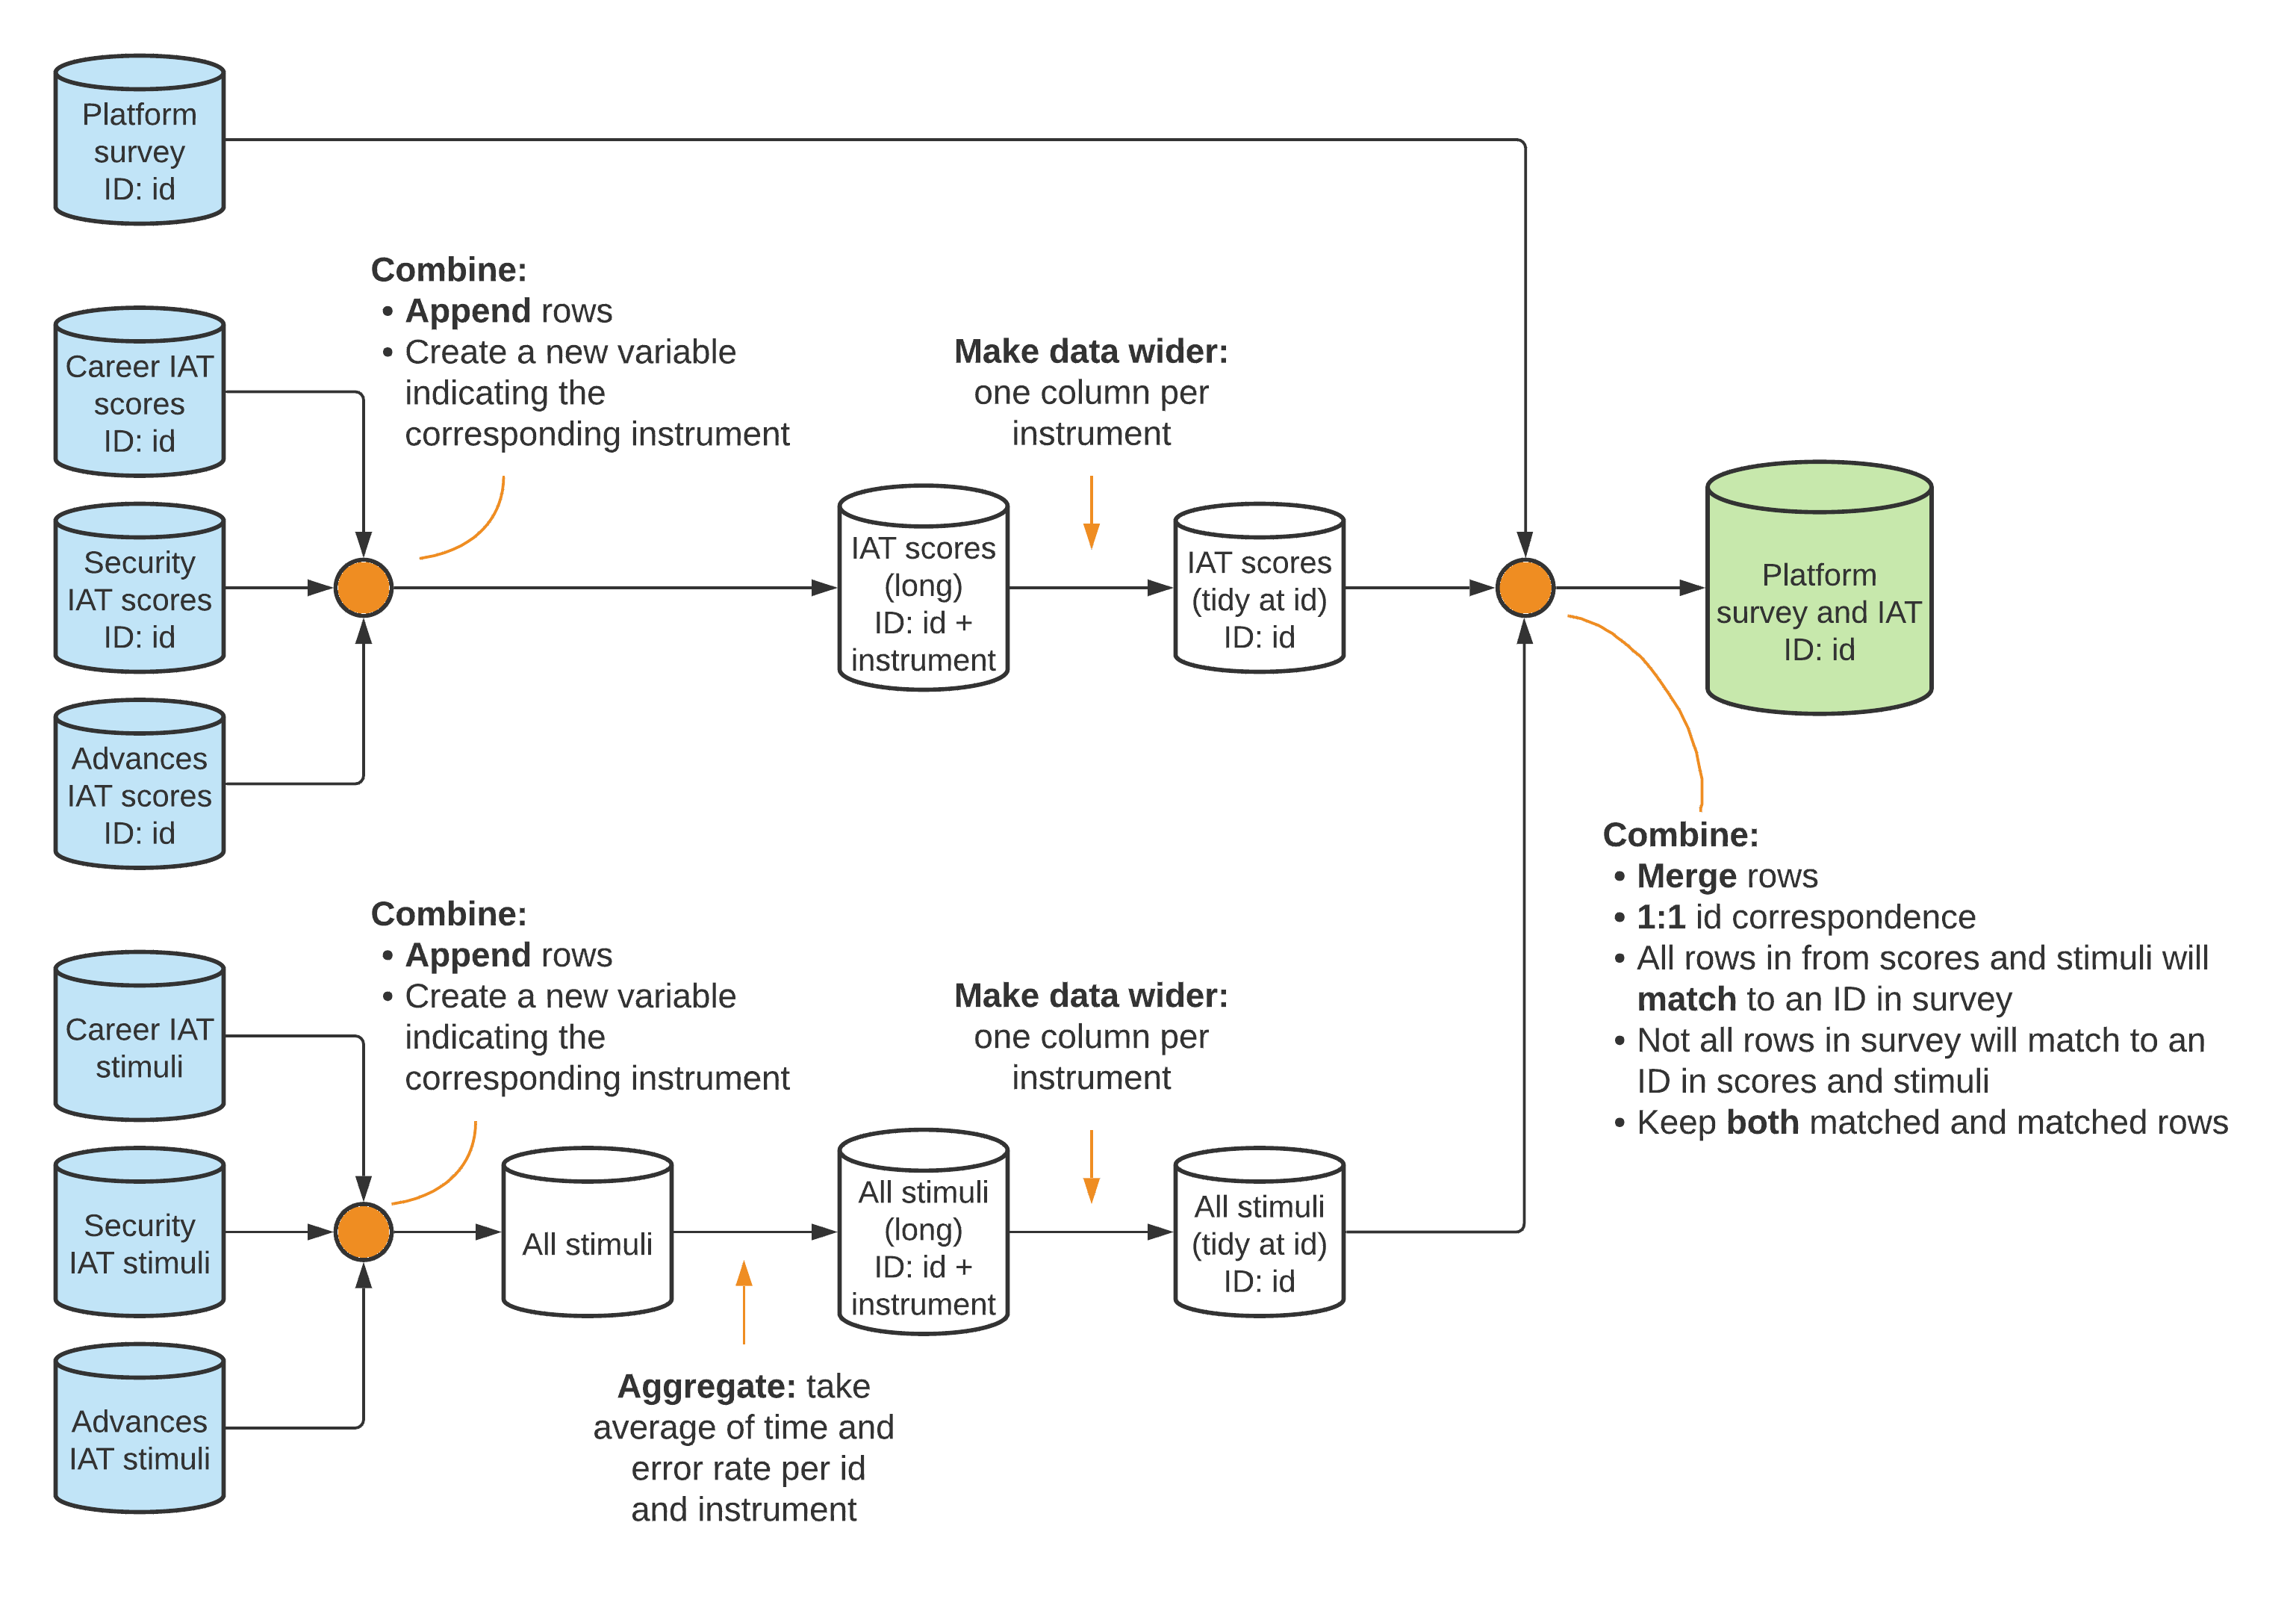
\includegraphics{examples/data-flow-chart.png}

\begin{quote}
The complete project data map is available at \url{https://git.io/Jtg3J}.
\end{quote}
\end{ex}

\hypertarget{translating-research-design-to-data-needs}{%
\section*{Translating research design to data needs}\label{translating-research-design-to-data-needs}}
\addcontentsline{toc}{section}{Translating research design to data needs}

An important step in translating the research design to specific data
structure is to determine which research design variables you will need in the data analysis
to infer what differences in measurement variables
are attributable to your research design.\index{research design variables}
These data needs should be expressed in your data map by
listing the data source for each variable in the data linkage table,
by adding columns for them in your master dataset
(the master dataset might not have any observations yet; that is not a problem),
and by indicating in your data flowcharts how they will be merged to the analysis data.
It is important you do this before acquiring any data,
to make sure that the data acquisition activities described in Chapter \ref{acquisition}
will generate the data needed to answer your research questions.

As DIME primarily works on impact evaluations,
we focus our discussion here on research designs
that compare a group that received
some kind of \textbf{treatment}\index{treatment}\footnote{\textbf{Treatment:} The general word for the evaluated intervention or event.
  This includes things like being offered a training,
  a cash transfer from a program,
  or experiencing a natural disaster, among many others.}
against a \textbf{counterfactual}\index{counterfactual}.\footnote{\textbf{Counterfactual:} A statistical description of
  what would have happened
  to specific individuals in an alternative scenario,
  for example, a different treatment assignment outcome.}
The key assumption is that each
person, facility, or village
(or whatever the unit of treatment is)
had two possible states: their outcome if they did receive the treatment
and their outcome if they did not receive that treatment.
The average impact of the treatment,\footnote{\textbf{Average treatment effect (ATE):}
  The expected average change in outcome
  that untreated units would have experienced
  had they been treated.}
is defined as the difference
between these two states averaged over all units.

However, we can never observe the same unit
in both the treated and untreated state simultaneously,
so we cannot calculate these differences directly.
Instead, the treatment group is compared to a control group
that is statistically indistinguishable,
which is often referred to as achieving
\textbf{balance} between two or more groups.
DIME Analytics maintains a Stata command to
standardize and automate the creation of well-formatted balance tables:
\texttt{iebaltab}.\footnote{Read more about how to install and use \texttt{iebaltab}
  and how it simplifies balance tables in Stata on the DIME Wiki:
  \url{https://dimewiki.worldbank.org/iebaltab}.}
Each research design has a different method for
identifying and balancing the counterfactual group.
The rest of this section covers how research data requirements
differ between those different methods.
What does not differ, however,
is that these data requirements are all research design variables.
And that the research design variables discussed below
should always be included in the master dataset.
You will often have to merge
the research design variables to other datasets,
but that is an easy task
if you created a data linkage table.

We assume you have a working familiarity
with the research designs mentioned here.
You should reference \textbf{Appendix \ref{design}},
where you will find more details
and specific references for common impact evaluation designs.

\hypertarget{applying-common-research-designs-to-data}{%
\subsection*{Applying common research designs to data}\label{applying-common-research-designs-to-data}}
\addcontentsline{toc}{subsection}{Applying common research designs to data}

In \textbf{experimental research designs},
such as \textbf{randomized control trials (RCTs)},\footnote{More details on RCTs and links to even more extensive resources
  can be found on the DIME Wiki:
  \url{https://dimewiki.worldbank.org/Randomized_Control_Trials}.}
\index{randomized control trials}\index{experimental research designs}
the research team determines which members
of the studied population will receive the treatment.
This is typically done by a randomized process
in which a subset of the eligible population
is randomly assigned to receive the treatment
(see later in this chapter for how to implement this).
The intuition is that if everyone in the eligible population
is assigned at random to either the treatment or control group,
then the two groups will, on average, be statistically indistinguishable.
Randomization makes it generally possible to obtain unbiased estimates of
the effects that can be attributed to a specific program or intervention:
in a randomized trial, the expected spurious correlation between treatment and outcomes
will approach zero as the sample size increases.\footnote{Duflo, Glennerster, and Kremer (\protect\hyperlink{ref-duflo2007using}{2007}), Gibson and Sautmann (\protect\hyperlink{ref-JPAL2020rct}{2020})}
The randomized assignment should be done
using data from the master dataset,
and the result should be saved back to the master dataset,
before being merged to other datasets.

\textbf{Quasi-experimental research designs},\footnote{More details on quasi-experimental research designs
  and links to even more extensive resources
  can be found on the DIME Wiki:
  \url{https://dimewiki.worldbank.org/Quasi-Experimental_Methods}}
\index{quasi-experimental research designs}
by contrast, are based on events not controlled by the research team.
Instead, they rely on ``experiments of nature'',
in which natural variation in exposure to treatment
can be argued to approximate deliberate randomization.
You must have a way to measure this natural variation,
and how the variation is categorized as outcomes of a naturally randomized assignment
must be documented in your master dataset.
Unlike carefully planned experimental designs,
quasi-experimental designs typically require the luck
of having access to data collected at the right times and places
to exploit events that occurred in the past.
Therefore, these methods often use either secondary data,
including administrative data or other classes of routinely-collected information,
and it is important that your data linkage table documents
how this data can be linked to the rest of the data in your project.

No matter the design type, you should be very clear about
which data points you observe or collect are research design variables.
For example,
\textbf{regression discontinuity (RD)}\footnote{More details on RD designs
  and links to even more extensive resources
  can be found on the DIME Wiki:
  \url{https://dimewiki.worldbank.org/Regression_Discontinuity}.}
\index{regression discontinuity}
designs exploit sharp breaks or limits
in policy designs.\footnote{See Alix-Garcia et al. (\protect\hyperlink{ref-alix2019can}{2019}) for an example.}
The cutoff determinant, or running variable,
should be saved in your master dataset.
In \textbf{instrumental variables (IV)}\footnote{More details on IV designs
  and links to even more extensive resources
  can be found on the DIME Wiki:
  \url{https://dimewiki.worldbank.org/Instrumental_Variables}.}
\index{instrumental variables}
designs, the \textbf{instruments} influence the \emph{probability} of treatment.\footnote{See Calderon, Iacovone, and Juarez (\protect\hyperlink{ref-calderon2017opportunity}{2017}) for an example.}
These research design variables should be collected
and stored in the master dataset.
Both the running variable in RD designs
and the instruments in IV designs,
are among the rare examples of research design variables
that may vary over time.
In such cases your research design should
ex-ante clearly indicate what point of time they will be recorded,
and this should be clearly documented in your master dataset.

In \textbf{matching} designs, observations are often grouped
by a strata, grouping, index, or propensity score.\footnote{More details on matching methods
  and links to even more extensive resources
  can be found on the DIME Wiki:
  \url{https://dimewiki.worldbank.org/Matching}.}
Like all research design variables, the matching results
should be stored in the master dataset.
This is best done by assigning a matching ID
to each matched pair or group,
and create a variable in the master dataset
with the matching ID each unit belongs to.\footnote{See Prennushi and Gupta (\protect\hyperlink{ref-prennushi2014women}{2014}) for an example.}
In all these designs, fidelity to the design is important to record as well.\footnote{See Pradhan et al. (\protect\hyperlink{ref-pradhan2013evaluating}{2013}) for an example.}
A program intended for students that scored under 50\% on a test
might have some cases where the program is offered to someone that scored 51\% at the test,
or someone that scored 49\% at the might decline to participate in the program.
Differences between assignments and realizations
should also be recorded in the master datasets.

\hypertarget{including-multiple-time-periods}{%
\subsection*{Including multiple time periods}\label{including-multiple-time-periods}}
\addcontentsline{toc}{subsection}{Including multiple time periods}

Your data map should also take into consideration
whether your project uses data from one time period or several.
A study that observes data in only one time period is called
a \textbf{cross-sectional study}.\index{cross-sectional data}
Observations over multiple time periods,
referred to as \textbf{longitudinal data}\index{longitudinal data},
can consist of either
\textbf{repeated cross-sections}\index{repeated cross-sectional data}
or \textbf{panel data}\index{panel data}.
In repeated cross-sections,
each successive round of data collection uses a new random sample
of observations from the treatment and control groups,
but in a panel data study
the same observations are tracked and included each round.\footnote{See Kondylis et al. (\protect\hyperlink{ref-kondylis2016female}{2016}) for an example.}
If each round of data collection is a separate activity,
then they should be treated as separate sources of data
and get their own row in the data linkage table.

If the data is generated continuously,
or acquired at frequent intervals,
then it can be treated as a single data source.
When panel data is acquired in discreet batches,
the data linkage table must document
how the different rounds will be merged or appended.
You must keep track of the \emph{attrition rate} in panel data,
which is the share of observations not observed in follow-up data.
It is common that the observations not possible to track
can be correlated with the outcome you study.\footnote{See Bertrand et al. (\protect\hyperlink{ref-bertrand2017contemporaneous}{2017}) for an example.}
For example, poorer households may live in more informal dwellings,
patients with worse health conditions might not survive to follow-up,
and so on.
If this is the case,
then your results might only be an effect of your remaining sample
being a subset of the original sample
that were better or worse off from the beginning.
You should have a variable in your master dataset
that indicates attrition.
A balance check using the attrition variable
can provide insights as to whether the lost observations
were systematically different
compared to the rest of the sample.

\hypertarget{incorporating-monitoring-data}{%
\subsection*{Incorporating monitoring data}\label{incorporating-monitoring-data}}
\addcontentsline{toc}{subsection}{Incorporating monitoring data}

For any study with an ex-ante design,
\textbf{monitoring data}\index{monitoring data}\footnote{More details on monitoring data can be found on the DIME Wiki:
  \url{https://dimewiki.worldbank.org/Administrative_and_Monitoring_Data\#Monitoring_Data}}
is very important for understanding if the
research design corresponds to reality.
The most typical example is to make sure that,
in an experimental design,
the treatment was implemented according to your treatment assignment.
Treatment implementation is often carried out by partners,
and field realities may be more complex than foreseen during research design.
Furthermore, the field staff of your partner organization,
might not be aware that their actions are the implementation of a research design.

Therefore, you must acquire monitoring data that
tells you how well the realized treatment implementation in the field
corresponds to your intended treatment assignment,
for nearly all experimental research designs.
While monitoring data has traditionally been collected by sending someone to the field ,
it is increasingly common to collect monitoring data remotely.
Some examples of remote monitoring include:
local collaborators uploading geotagged images for visible interventions (such as physical infrastructure),
installing sensors to broadcast measurements (such as air pollution or waterflow),
distributing wearable devices to track location or physical activity (such as fitbits),
or applying image recognition to satellite data.
In-person monitoring activities are often preferred but
cost and travel dangers, such as conflicts or disease outbreaks,
make remote monitoring innovations increasingly appealing.
If cost alone is the constraint,
consider sampling a subset of the implementation area to monitor in-person.
This may not be detailed enough to be used as a control in your analysis,
but it will still provide a means to
estimate the validity of your research design assumptions.

Linking monitoring data to the rest of the data in your project
is often complex and a major source of errors.
Monitoring data is rarely received in the same format or structure as your research data.\footnote{See Goldstein et al. (\protect\hyperlink{ref-goldstein2015formalizing}{2015}) for an example.}
For example, you may receive a list of the names of all people who attended a training,
or administrative data from a partner organization without a proper identifier.
In both those cases it can be difficult to ensure a one-to-one match
between units in the monitoring data and the master datasets.
Planning ahead, and collaborating closely with the implementing
organization from the outset of the project,
is the best way to avoid these difficulties.
Often, it is ideal for the research team to prepare forms (paper or electronic) for monitoring,
preloading with names of sampled individuals,
or ensuring that there is a consistent identifier that is directly linkable to the project ID.
If monitoring data is not handled carefully, you risk ending up with poor correlation
between treatment uptake and treatment assignment,
without a way to tell if the poor correlation is just
a result of poor matching of the monitoring data or a meaningful implementation problem.

\hypertarget{creating-research-design-variables-by-randomization}{%
\section*{Creating research design variables by randomization}\label{creating-research-design-variables-by-randomization}}
\addcontentsline{toc}{section}{Creating research design variables by randomization}

Random sampling and random treatment assignment
are two core research activities
that generate important research design variables.
Random sampling and random treatment assignment directly determine
the set of individuals who will be observed
and what their status will be for the purpose of effect estimation.
\textbf{Randomization}\footnote{\textbf{Randomization} is often used interchangeably
  to mean random treatment assignment.
  In this book however, \emph{randomization} will only
  be used to describe the process of generating
  a sequence of unrelated numbers, i.e.~a random process.
  \emph{Randomization} will never be used to mean
  the process of assigning units in treatment and control groups,
  that will always be called \emph{random treatment assignment},
  or a derivative thereof.}
is used to ensure that a sample is representative and
that treatment groups are statistically indistinguishable.

Randomization in statistical software is non-trivial
and its mechanics are unintuitive for the human brain.
The principles of randomization we will outline
apply not just to random sampling and random assignment,
but to all statistical computing processes that have random components
such as simulations and bootstrapping.
Furthermore, all random processes introduce statistical noise
or uncertainty into estimates of effect sizes.
Choosing one random sample from all the possibilities produces some probability of
choosing a group of units that are not, in fact, representative.
Similarly, choosing one random assignment produces some probability of
creating groups that are not good counterfactuals.
\emph{Power calculation} and \emph{randomization inference}
are the main methods by which these probabilities of error are assessed.
These analyses are particularly important in the initial phases of development research --
typically conducted before any data acquisition or field work occurs --
and have implications for feasibility, planning, and budgeting.

\hypertarget{randomizing-sampling-and-treatment-assignment}{%
\subsection*{Randomizing sampling and treatment assignment}\label{randomizing-sampling-and-treatment-assignment}}
\addcontentsline{toc}{subsection}{Randomizing sampling and treatment assignment}

\textbf{Sampling} is the process of randomly selecting observations
from a list of individuals to create a representative or statistically similar sub-sample.\index{sampling}
This process can be used, for example, to select a subset from all eligible units
to be included in data collection when the cost of collecting data on everyone is prohibitive.\footnote{More details on sampling and important consideration related to sample size,
  as well as links to even more extensive resources
  can be found on the DIME Wiki:
  \url{https://dimewiki.worldbank.org/Sample_Size_and_Power_Calculations}.}
But it can also be used to select a sub-sample of your observations to test a computationally heavy process
before running it on the full data.
\textbf{Randomized treatment assignment} is the process of assigning observations to different treatment arms.
This process is central to experimental research design.
Most of the code processes used for randomized assignment are the same as those used for sampling,
since it is also a process of randomly splitting a list of observations into groups.
Where sampling determines whether a particular individual
will be observed at all in the course of data collection,
randomized assignment determines if each individual will be observed
as a treatment observation or used as a counterfactual.

The list of units to sample or assign from may be called a \textbf{sampling universe},
a \textbf{listing frame}, or something similar.
The starting point for randomized sampling or assignment
should be a \textbf{master dataset} in almost all cases,
and the result of the randomized process should always be saved in the master dataset
before it is merged to any other data.
Example of exceptions
when this cannot start from a master dataset are:
sampling done in real time, such as randomly sampling patients
as they arrive at a health facility, and
treatment assignment done through an in-person lottery.
In those cases,
it is important that you collect enough data
during the real time sampling,
or take care to prepare the inputs for the lottery
such that you can add these individuals
to your master dataset afterwards.

The simplest form of sampling is
\textbf{uniform-probability random sampling}.
This means that every eligible observation in the master dataset
has an equal probability of being selected.
The most explicit method of implementing this process
is to assign random numbers to all your potential observations,
order them by the number they are assigned,
and mark as ``sampled'' those with the lowest numbers, up to the desired proportion.
There are a number of shortcuts to doing this process,
but they all use this method as the starting point,
so you should become familiar with exactly how it works.
The do-file below provides an example of
how to implement uniform-probability sampling in practice.
This code uses a Stata built-in dataset and is fully reproducible
(more on reproducible randomization in next section),
so anyone that runs this code in any version of Stata later than 13.1
(the version set in this code)
will get the exact same, but still random, results.

\begin{Shaded}
\begin{Highlighting}[numbers=left,,]
\NormalTok{* Set up reproducible randmomization - VERSIONING, SORTING and SEEDING}
\NormalTok{    ieboilstart , v(13.1)    }\CommentTok{// Version}
    \OtherTok{`r(version)'}             \CommentTok{// Version}
    \KeywordTok{sysuse}\NormalTok{ bpwide.dta, }\KeywordTok{clear} \CommentTok{// Load data}
    \KeywordTok{isid}\NormalTok{ patient, }\KeywordTok{sort}       \CommentTok{// Sort}
    \KeywordTok{set} \DecValTok{seed}\NormalTok{ 215597          }\CommentTok{// Seed - drawn using https://bit.ly/stata-random}

\NormalTok{* Generate a random number and }\KeywordTok{use}\NormalTok{ it to }\KeywordTok{sort}\NormalTok{ the observations.}
\NormalTok{* Then the }\KeywordTok{order}\NormalTok{ the observations are sorted }\KeywordTok{in}\NormalTok{ is random.}
    \KeywordTok{gen}\NormalTok{ sample_rand = rnormal() }\CommentTok{// Generate a random number}
    \KeywordTok{sort}\NormalTok{ sample_rand            }\CommentTok{// Sort based on the random number}

\NormalTok{* Use the }\KeywordTok{sort} \KeywordTok{order}\NormalTok{ to }\KeywordTok{sample}\NormalTok{ 20% (0.20) }\KeywordTok{of}\NormalTok{ the observations.}
\NormalTok{*_N }\KeywordTok{in}\NormalTok{ Stata is the number }\KeywordTok{of}\NormalTok{ observations }\KeywordTok{in}\NormalTok{ the active dataset,}
\NormalTok{* and }\DataTypeTok{_n}\NormalTok{ is the }\OtherTok{row}\NormalTok{ number }\KeywordTok{for}\NormalTok{ each observation. The bpwide.dta has 120}
\NormalTok{* observations and 120*0.20 = 24, so (}\DataTypeTok{_n}\NormalTok{ <= _N * 0.20) is 1 }\KeywordTok{for}\NormalTok{ observations}
\NormalTok{* with a }\OtherTok{row}\NormalTok{ number equal to }\KeywordTok{or}\NormalTok{ less than 24, and 0 }\KeywordTok{for} \OtherTok{all}\NormalTok{ other}
\NormalTok{* observations. Since the }\KeywordTok{sort} \KeywordTok{order}\NormalTok{ is randomized, }\KeywordTok{this} \KeywordTok{means}\NormalTok{ that we}
\NormalTok{* have randomly sampled 20% }\KeywordTok{of}\NormalTok{ the observations.}
    \KeywordTok{gen} \KeywordTok{sample}\NormalTok{ = (}\DataTypeTok{_n}\NormalTok{ <= _N * 0.20)}

\NormalTok{* Restore the original }\KeywordTok{sort} \KeywordTok{order}
    \KeywordTok{isid}\NormalTok{ patient, }\KeywordTok{sort}

\NormalTok{* Check your result}
    \KeywordTok{tab} \KeywordTok{sample}
\end{Highlighting}
\end{Shaded}

Sampling typically has only two possible outcomes: observed and unobserved.
Similarly, a simple randomized assignment has two outcomes: treatment and control,
and the logic in the code would be identical to the sampling code example.
However, randomized assignment often involves multiple treatment arms
which each represent different varieties of treatments to be delivered;\footnote{See De Andrade, Bruhn, and McKenzie (\protect\hyperlink{ref-de2013helping}{2013}) for an example.}
in some cases, multiple treatment arms are intended to overlap in the same sample.
Complexity can therefore grow very quickly in randomized assignment
and it is doubly important to fully understand the conceptual process
that is described in the experimental design,
and fill in any gaps before implementing it in code.
The do-file below provides an example of how to implement
a randomized assignment with multiple treatment arms.

\begin{Shaded}
\begin{Highlighting}[numbers=left,,]
\NormalTok{* Set up reproducible randomization - VERSIONING, SORTING and SEEDING}
\NormalTok{    ieboilstart , v(13.1)    }\CommentTok{// Version}
    \OtherTok{`r(version)'}             \CommentTok{// Version}
    \KeywordTok{sysuse}\NormalTok{ bpwide.dta, }\KeywordTok{clear} \CommentTok{// Load data}
    \KeywordTok{isid}\NormalTok{ patient, }\KeywordTok{sort}       \CommentTok{// Sort}
    \KeywordTok{set} \DecValTok{seed}\NormalTok{ 654697          }\CommentTok{// Seed - drawn using https://bit.ly/stata-random}

\NormalTok{* Generate a random number and }\KeywordTok{use}\NormalTok{ it to }\KeywordTok{sort}\NormalTok{ the observation.}
\NormalTok{* Then the }\KeywordTok{order}\NormalTok{ the observations are sorted }\KeywordTok{in}\NormalTok{ is random.}
    \KeywordTok{gen}\NormalTok{ treatment_rand = rnormal() }\CommentTok{// Generate a random number}
    \KeywordTok{sort}\NormalTok{ treatment_rand            }\CommentTok{// Sort based on the random number}

\NormalTok{* See simple-}\KeywordTok{sample}\NormalTok{.}\KeywordTok{do}\NormalTok{ example }\KeywordTok{for}\NormalTok{ an explanation }\KeywordTok{of} \StringTok{"(_n <= _N * X)"}\NormalTok{.}
\NormalTok{* The code below randomly selects one third }\KeywordTok{of}\NormalTok{ the observations into }\FunctionTok{group}\NormalTok{ 0,}
\NormalTok{* one third into }\FunctionTok{group}\NormalTok{ 1 and one third into }\FunctionTok{group}\NormalTok{ 2.}
\NormalTok{* Typically 0 represents the control }\FunctionTok{group}
\NormalTok{* and 1 and 2 represents the }\KeywordTok{two}\NormalTok{ treatment arms}
    \KeywordTok{generate}\NormalTok{ treatment = 0                       }\CommentTok{// Set all observations to 0 (control)}
    \KeywordTok{replace}\NormalTok{  treatment = 1 }\KeywordTok{if}\NormalTok{ (}\DataTypeTok{_n}\NormalTok{ <= _N * (2/3)) }\CommentTok{// Set only the first two thirds to 1}
    \KeywordTok{replace}\NormalTok{  treatment = 2 }\KeywordTok{if}\NormalTok{ (}\DataTypeTok{_n}\NormalTok{ <= _N * (1/3)) }\CommentTok{// Set only the first third to 2}

\NormalTok{* Restore the original }\KeywordTok{sort} \KeywordTok{order}
    \KeywordTok{isid}\NormalTok{ patient, }\KeywordTok{sort}

\NormalTok{* Check your result}
    \KeywordTok{tab}\NormalTok{ treatment}
\end{Highlighting}
\end{Shaded}

\hypertarget{programming-reproducible-random-processes}{%
\subsection*{Programming reproducible random processes}\label{programming-reproducible-random-processes}}
\addcontentsline{toc}{subsection}{Programming reproducible random processes}

For statistical programming to be reproducible,
you must be able to re-obtain its exact outputs in the future.\footnote{Orozco et al. (\protect\hyperlink{ref-orozco2018make}{2018})}
We will focus on what you need to do to produce
truly random results for your project,
to ensure you can get those results again.
This takes a combination of strict rules, solid understanding, and careful programming.
This section introduces strict rules:
these are non-negotiable (but thankfully simple).
Stata, like most statistical software, uses a \textbf{pseudo-random number generator}\footnote{\textbf{Pseudo-random number generator:} An algorithm that creates a long, fixed sequence of numbers
  which exhibits no statistical relationships between the position or value of any set of those numbers.}
which, in ordinary research use,
produces sequences of number that are as good as random.\footnote{More details on randomization in Stata
  and the three important steps that needs to be followed
  to make it reproducible can be found on the DIME Wiki:
  \url{https://dimewiki.worldbank.org/Randomization_in_Stata}.}
However, for \emph{reproducible} randomization, we need two additional properties:
we need to be able to fix the sequence of numbers generated and
we need to ensure that the first number is independently randomized.
In Stata, this is accomplished through three concepts:
\textbf{versioning}, \textbf{sorting}, and \textbf{seeding}.
We again use Stata in our examples,
but the same principles translate to all other programming languages.

\begin{itemize}
\tightlist
\item
  \textbf{Rule 1: Versioning} requires using the same version of the software each time you run the random process.
  If anything is different, the underlying list of random numbers may have changed,
  and it may be impossible to recover the original result.
  In Stata, the \texttt{version} command ensures that the list of random numbers is fixed.\footnote{At the time of writing, we recommend using \texttt{version\ 13.1} for backward compatibility;
    the algorithm used to create this list of random numbers was changed after Stata 14 but the improvements do not matter in practice.}
  The \texttt{ieboilstart} command in \texttt{ietoolkit} provides functionality to support this requirement.\footnote{Read more about how to install and use \texttt{ieboilstart}
    and how this command can help you
    harmonize settings such as version across users on the DIME Wiki:
    \url{https://dimewiki.worldbank.org/ieboilstart}.}
  We recommend you use \texttt{ieboilstart} at the beginning of your master do-file.\footnote{More details and description of each section of our template master do-file
    can be found on the DIME Wiki:
    \url{https://dimewiki.worldbank.org/Master_Do-files}.}
  Note that testing your do-files without running them
  via the master do-file may produce different results,
  since Stata's \texttt{version} setting expires after each time you run your do-files.
\end{itemize}

\begin{itemize}
\tightlist
\item
  \textbf{Rule 2: Sorting} requires that the order of the actual data that the random process is run on is fixed.
  Because random numbers are assigned to each observation row-by-row starting from
  the top row,
  changing their order will change the result of the process.
  In Stata, we recommend using \texttt{isid\ {[}id\_variable{]},\ sort}
  to guarantee a unique sorting order.
  This command does two things.
  First it tests that all observations have unique values in the sort variable,
  as duplicates would cause an ambiguous sort order.
  If all values are unique,
  then the command sorts on this variable guaranteeing a unique sort order.
  It is a common misconception that the \texttt{sort,\ stable} command
  may also be used,
  but by itself it cannot guarantee an unambiguous sort order
  and is therefore not appropriate for this purpose.
  Since the exact order must be unchanged,
  the underlying data itself must be unchanged as well between runs.
  This means that if you expect the number of observations to change
  (for example to increase during ongoing data collection),
  your randomization will not be reproducible unless you split your data up into
  smaller fixed datasets where the number of observations does not change.
  You can combine all
  those smaller datasets after your randomization.
\end{itemize}

\begin{itemize}
\tightlist
\item
  \textbf{Rule 3: Seeding} requires manually setting the start point in the list of pseudo-random numbers.
  A seed is just a single number that specifies one of the possible start points.
  It should be at least six digits long and you should use exactly
  one unique, different, and randomly created seed per randomization process.\footnote{You can draw a uniformly distributed six-digit seed randomly by visiting \url{https://bit.ly/stata-random}.
    (This link is a just shortcut to request such a random number on \url{https://www.random.org}.)
    There are many more seeds possible but this is a large enough set for most purposes.}
  In Stata, \texttt{set\ seed\ {[}seed{]}} will set the generator
  to the start point identified by the seed.
  In R, the \texttt{set.seed} function does the same.
  To be clear: you should not set a single seed once in the master do-file,
  but instead you should set a new seed in code right before each random process.
  The most important thing is that each of these seeds is truly random,
  so do not use shortcuts such as the current date or a seed you have used before.
  You should also describe in your code how the seed was selected.
\end{itemize}

You must carefully confirm exactly how your code runs before finalizing it,
as other commands may induce randomness in the data,
change the sorting order,
or alter the place of the random generator without you realizing it.
To confirm that a randomization has worked correctly before finalizing its results,
save the outputs of the process in a temporary location,
re-run the code, and use \texttt{cf} or \texttt{datasignature} to ensure
nothing has changed. It is also advisable to let someone else reproduce your
randomization results on their machine to remove any doubt that your results
are reproducible.
Once the result of a randomization is used in the field,
there is no way to correct any mistakes.
The code below provides an example of a fully reproducible randomization.

\begin{Shaded}
\begin{Highlighting}[numbers=left,,]
\NormalTok{* VERSIONING - Set the }\KeywordTok{version}
\NormalTok{    ieboilstart , v(13.1)}
    \OtherTok{`r(version)'}

\NormalTok{* Load the auto dataset (auto.dta is a }\KeywordTok{test}\NormalTok{ dataset included }\KeywordTok{in} \OtherTok{all}\NormalTok{ Stata installations)}
    \KeywordTok{sysuse}\NormalTok{ auto.dta , }\KeywordTok{clear}

\NormalTok{* SORTING - }\KeywordTok{sort} \KeywordTok{on}\NormalTok{ the uniquely identifying }\KeywordTok{variable} \StringTok{"make"}
    \KeywordTok{isid}\NormalTok{ make, }\KeywordTok{sort}

\NormalTok{* SEEDING - Seed picked }\KeywordTok{using}\NormalTok{ https:}\CommentTok{//bit.ly/stata-random}
    \KeywordTok{set} \DecValTok{seed}\NormalTok{ 287608}

\NormalTok{* Demonstrate stability after VERSIONING, SORTING and SEEDING}
    \KeywordTok{gen}\NormalTok{ check1 = rnormal()  }\CommentTok{// Create random number}
    \KeywordTok{gen}\NormalTok{ check2 = rnormal()  }\CommentTok{// Create a second random number without resetting seed}

    \KeywordTok{set} \DecValTok{seed}\NormalTok{ 287608         }\CommentTok{// Reset the seed}
    \KeywordTok{gen}\NormalTok{ check3 = rnormal()  }\CommentTok{// Create a third random number after resetting seed}

\NormalTok{* Visualize randomization results. See how check1 and check3 are identical,}
\NormalTok{* but check2 is random relative to check1 and check3}
    \KeywordTok{graph} \FunctionTok{matrix}\NormalTok{ check1 check2 check3 , half}
\end{Highlighting}
\end{Shaded}

As discussed above, at times it will not be possible to use a master dataset for
randomized sampling or treatment assignment
(examples were sampling patients on arrival or live lotteries).
In addition to presenting challenges with matching,
these methods typically do not leave a record of the randomization,
and as such are never reproducible.
However, you can often run your randomization in advance
even when you do not have list of eligible units in advance.
Let's say you want to, at various health facilities,
randomly select a sub-sample of patients as they arrive.
You can then have a pre-generated list
with a random order of ``in sample'' and ``not in sample''.
Your field staff would then go through this list in order
and cross off one randomized result as it is used for a patient.

This is especially beneficial if you are implementing a more complex randomization.
For example, a hypothetical research design may call for enumerators to:

\begin{enumerate}
\def\labelenumi{\arabic{enumi}.}
\tightlist
\item
  sample 10\% of people observed in a particular location;
\item
  show a video to 50\% of the sample;
\item
  administer a short questionnaire to 80\% of all those sampled; and
\item
  administer a longer questionnaire to the remaining 20\%, with the questionnaire mix equal between those who were shown the video and those that were not.
\end{enumerate}

In real-time, such a complex randomization is much more likely to be implemented correctly
if your field staff simply can follow a list with the randomized categories
where you are in control of the pre-determined proportions and the random order.
This way, you can also control with precision
how these categories are evenly distributed across all the locations
where you plan to conduct this research.

Finally, if this real-time randomization implementation is done using survey software,
then the pre-generated list of randomized categories can be preloaded
into the questionnaire.
Then the field team can follow a list of respondent IDs
that are randomized into the appropriate categories,
and the survey software can show a video and control which version of the questionnaire is asked.
This way, you reduce the risk of errors in field randomization.

\hypertarget{implementing-clustered-or-stratified-designs}{%
\subsection*{Implementing clustered or stratified designs}\label{implementing-clustered-or-stratified-designs}}
\addcontentsline{toc}{subsection}{Implementing clustered or stratified designs}

For a variety of reasons, random sampling and random treatment assignment
are rarely as straightforward as a uniform-probability draw.
The most common variants are \textbf{clustering} and \textbf{stratification}.\footnote{Athey and Imbens (\protect\hyperlink{ref-athey2017econometrics}{2017}\protect\hyperlink{ref-athey2017econometrics}{a})}
\textbf{Clustering} occurs when your unit of analysis is different
than the unit of sampling or treatment assignment.\footnote{More details on the concepts of unit of sampling
  and unit treatment assignment
  can be found on the DIME Wiki:
  go to \url{https://dimewiki.worldbank.org/Unit_of_Observation}}
For example, a policy may be implemented at the village level,
or you may only be able to send enumerators to a limited number of villages,
or the outcomes of interest for the study are measured at the household level.\footnote{More details on clustered sampling and
  links to additional resources can be found on the DIME Wiki:
  \url{https://dimewiki.worldbank.org/Multi-stage_(Cluster)_Sampling}.}
\index{clustered randomization}
The groups in which units are assigned to treatment are called clusters.\footnote{See Keating et al. (\protect\hyperlink{ref-keating2011evaluating}{2011}) for an example.}

\textbf{Stratification} breaks the full set of observations into subgroups
before performing randomized assignment within each subgroup.\footnote{More details on stratified sampling and
  links to additional resources can be found on the DIME Wiki:
  \url{https://dimewiki.worldbank.org/Stratified_Random_Sample}.}
\index{stratification}
The subgroups are called \textbf{strata}.
This ensures that members of every subgroup
are included in all groups of the randomized assignment process,
or that members of all groups are observed in the sample.
Without stratification, it is possible that the randomization
would put all the members of a subgroup into just one of the treatment arms,
or fail to select any of them into the sample.
For both clustering and stratification,
implementation is nearly identical in both random sampling and random assignment.

Clustering is procedurally straightforward in Stata,
although it typically needs to be performed manually.
To cluster a sampling or randomized assignment,
randomize on the master dataset for the unit of observation of the cluster,
and then merge the results to the master dataset for the unit of analysis.
This is a many-to-one merge and your data map should document
how those datasets can be merged correctly.
If you do not have a master dataset yet for the unit of observation of the cluster,
then you first have to create that and update your data map accordingly.
When sampling or randomized assignment is conducted using clusters,
the clustering variable should be clearly identified in the master dataset
for the unit of analysis
since it will need to be used in subsequent statistical analysis.
Namely, standard errors for these types of designs must be clustered
at the level at which the randomization was clustered.\footnote{\url{https://blogs.worldbank.org/impactevaluations/when-should-you-cluster-standard-errors-new-wisdom-econometrics-oracle}}
This accounts for the design covariance within the cluster --
the information that if one individual was observed or treated there,
the other members of the clustering group were as well.

Although procedurally straightforward,
implementing stratified designs in statistical software is prone to error.
Even for a simple multi-armed design,
the basic method of randomly ordering the observations
will often create very skewed assignments.\footnote{\url{https://blogs.worldbank.org/impactevaluations/tools-of-the-trade-doing-stratified-randomization-with-uneven-numbers-in-some-strata}}
The user-written \texttt{randtreat} command properly implements stratification.\footnote{Carril (\protect\hyperlink{ref-carril2017dealing}{2017})}
The options and outputs (including messages) from the command should be carefully reviewed
so that you understand exactly what has been implemented.
Notably, it is extremely hard to target precise numbers of observations
in stratified designs, because exact allocations are rarely round fractions
and the process of assigning the leftover ``misfit'' observations
imposes an additional layer of randomization above the specified division.

\hypertarget{performing-power-calculations}{%
\subsection*{Performing power calculations}\label{performing-power-calculations}}
\addcontentsline{toc}{subsection}{Performing power calculations}

Random sampling and treatment assignment are noisy processes:
it is impossible to predict the result in advance.
By design, we know that the exact choice of sample or treatment
will be uncorrelated with our key outcomes,
but this lack of correlation is only true ``in expectation'' --
that is, the noise component of the correlation between randomization and outcome
will only be zero on average across a large number of randomized trials.
In any \emph{particular} randomization,
the correlation between the sampling or randomized assignments and the outcome variable
is guaranteed to be \emph{nonzero}:
this is called the \textbf{in-sample} or \textbf{finite-sample correlation}.

Since we know that the true correlation
(over the ``population'' of potential samples or randomized assignments)
is zero, we think of the observed correlation as an \textbf{error}.
In sampling, we call this the \textbf{sampling error},
and it is defined as the difference between a true population parameter
and the observed mean due to chance selection of units.\footnote{More details on sampling and
  links to additional resources can be found on the DIME Wiki:
  \url{https://dimewiki.worldbank.org/Sampling}.}
In randomized assignment, we call this the \textbf{randomization noise},
and define it as the difference between a true treatment effect
and the estimated effect due to placing units in groups.
The intuition for both measures is that from any group,
you can find some possible subsets that have higher-than-average values of some measure;
similarly, you can find some that have lower-than-average values.
Your random sample or treatment assignment will fall in one of these categories,
and we need to assess the likelihood and magnitude of this occurrence.
\emph{Power calculation} and \emph{randomization inference} are the two key tools to doing so.\footnote{More details on how to perform power calculations
  can be found on the DIME Wiki:
  \url{https://dimewiki.worldbank.org/Sample_Size_and_Power_Calculations}.}

\textbf{Power calculations} report the likelihood that your experimental design
\index{power calculations}
will be able to detect the treatment effects you are interested in
given these sources of noise.
This measure of \textbf{power} can be described in various different ways,
each of which has different practical uses.
The purpose of power calculations is to identify where the strengths and weaknesses
of your design are located, so you know the relative tradeoffs you will face
by changing your randomization scheme for the final design.
It is important to consider take-up rates and attrition when doing power calculations;
incomplete take-up will significantly reduce power,
understanding what minimum level of take-up is required can help guide field operations
(for this reason, monitoring take-up in real-time is often critical).

The \textbf{minimum detectable effect (MDE)}\footnote{More details on minimum detectable effect and
  links to additional resources can be found on the DIME Wiki:
  \url{https://dimewiki.worldbank.org/Minimum_Detectable_Effect}.}
is the smallest true effect that a given research design can reliably detect.
This is useful as a check on whether a study is worthwhile.
If, in your field, a ``large'' effect is just a few percentage points
or a small fraction of a standard deviation,
then it is nonsensical to run a study whose MDE is much larger than that.
This is because, given the sample size and variation in the population,
the effect needs to be much larger to possibly be statistically detected,
so such a study would never be able to say anything about the effect size that is practically relevant.
Conversely, the \textbf{minimum sample size} pre-specifies expected effect sizes
and tells you how large a study's sample would need to be to detect that effect,
which can tell you what resources you would need
to implement a useful study.

\textbf{Randomization inference}\footnote{More details on randomization inference and
  links to additional resources can be found on the DIME Wiki:
  \url{https://dimewiki.worldbank.org/Randomization_Inference}.}
is used to analyze the likelihood
\index{randomization inference}
that the randomized assignment process, by chance,
would have created a false treatment effect as large as the one you estimated.
Randomization inference is a generalization of placebo tests,
because it considers what the estimated results would have been
from a randomized assignment that did not in fact happen in reality.
Randomization inference is particularly important
in quasi-experimental designs and in small samples,
where the number of possible \emph{randomizations} is itself small.
Randomization inference can therefore be used proactively during experimental design,
to examine the potential spurious treatment effects your exact design is able to produce.
If there is significant heaping at particular result levels,
or if results seem to depend dramatically on the outcomes for a small number of individuals,
randomization inference will flag those issues before the experiment is fielded
and allow adjustments to the design to be made.

\hypertarget{looking-ahead-3}{%
\section*{Looking ahead}\label{looking-ahead-3}}
\addcontentsline{toc}{section}{Looking ahead}

This chapter introduced the DIME Data Map template,
a toolkit to documents your data acquisition plan and
how each data source relates to the design of your study.
The data map contains research design variables and the instructions
for using them in combination with measurement variables, which together
will form the dataset(s) for your analytical work.
We then discussed ways for you to use this planning data
to inform and execute research design tasks,
such as randomized sampling and assignment,
and to produce concrete measures
of whether the project design is sufficient to answer the research questions you pose.
In the next chapter,
we will turn to the first step in actually answering those questions --
data acquisition.
The next chapter will detail the processes of obtaining
original data,
whether you are collecting it yourself or
receiving it from another entity.

\hypertarget{acquisition}{%
\chapter{Acquiring development data}\label{acquisition}}

Many research questions require the team to acquire original data,
because no source of publicly available data addresses the
inputs or outcomes of interest for the relevant population.
Data acquisition can take many forms, including:
primary data generated through surveys;
private sector partnerships granting access to new data sources, such as administrative and sensor data;
digitization of paper records, including administrative data; web scraping;
primary data capture by unmanned aerial vehicles or other types of remote sensing;
or novel integration of various types of datasets, such as combining survey and sensor data.
Much of the recent push toward credibility in the social sciences has focused on analytical practices.
However, credible development research depends, first and foremost, on the quality of the acquired data.
Clear and careful documentation of the data acquisition process is essential for research reproducibility.

This chapter covers reproducible data acquisition,
special considerations for generating high-quality survey data,
and protocols for safely and securely handling confidential data.
The first section discusses reproducible data acquisition:
how to establish and document your right to use the data.
This applies to all original data,
whether collected for the first time through surveys or sensors or acquired through a unique partnership.
The second section goes into detail on data acquisition through surveys,
as this process is typically more involved than acquisition of secondary data,
and has more in-built opportunities for quality control.
It provides detailed guidance on the electronic survey workflow,
from designing electronic survey instruments to monitoring data quality once fieldwork is ongoing.
The final section discusses safe data handling,
providing guidance on how to receive, transfer, store, and share confidential data.
Secure file management is a basic requirement to comply with the legal and
ethical agreements that allow access to personal information for research purposes.

\begin{summary}
\hypertarget{summary-acquiring-development-data}{%
\subsection*{Summary: Acquiring development data}\label{summary-acquiring-development-data}}
\addcontentsline{toc}{subsection}{Summary: Acquiring development data}

The process of obtaining research data is unique to every project. However, there are basic structures and processes that are common to both data acquired from others and data generated by surveys:

\textbf{1. When receiving data from others, ownership and licensing are critical.} Before any data is transferred, you should be certain of all formal rights associated with that data. This includes:

\begin{itemize}
\tightlist
\item
  Ensuring that the partner \emph{has the right} to share the data with you, especially if it contains PII
\item
  Identifying the \emph{data owner} and any restrictions the owner places on data use, storage, or handling
\item
  Securing a \emph{data use agreement or license} from the partner, outlining your rights and responsibilities regarding analysis, publication of results and derived data, re-distribution of data, and data destruction
\end{itemize}

\textbf{2. Collecting high-quality data} requires careful planning and attention to detail throughout the workflow. We cover best practices for all surveys, and detailed considerations for electronic surveys:

\begin{itemize}
\tightlist
\item
  Using the data map to \emph{produce and pilot draft instruments} on paper, to focus on survey content
\item
  \emph{Structuring questionnaires for electronic programming} and pilot for function, taking into consideration features like pagination, ordering, looping, conditional execution, and instructions for enumerators
\item
  \emph{Testing data outputs for analytical compatibility}, such as code-friendly variable and value labels
\item
  \emph{Training enumerators carefully}, using the paper survey before the electronic template, assessing performance objectively throughout training, and transparently selecting top performers for fieldwork
\item
  \emph{Assessing data quality in real-time}, through scripted high frequency checks and diligent field validation
\end{itemize}

\textbf{3. No matter how your data is acquired, secure data handling is essential.} This includes:

\begin{itemize}
\tightlist
\item
  \emph{Encrypting data} on all devices, \emph{in transit and at rest}, beginning from the point of collection and including all intermediate locations such as servers and local devices
\item
  \emph{Storing encryption keys} using appropriate password management software with strong, unique passwords for all applications and devices with access
\item
  \emph{Backing up data} in case of total loss or failure of hardware and software at any site
\end{itemize}

\hypertarget{takeaways-3}{%
\subsubsection*{Takeaways}\label{takeaways-3}}
\addcontentsline{toc}{subsubsection}{Takeaways}

\textbf{TTLs/PIs will:}

\begin{itemize}
\tightlist
\item
  Obtain appropriate legal documentation and permissions agreements for all data
\item
  For surveys: support translation of the data map to survey instruments; oversee instrument development
\item
  For surveys: Review and provide inputs to the project's data quality assurance plan
\item
  For surveys: Guide decisions on how to correct issues identified during data quality checks
\item
  Oversee implementation of security measures; manage access codes, encryption keys, and hardware
\item
  Determine and communicate institutionally-appropriate data storage and backup plans
\end{itemize}

\textbf{RAs will:}

\begin{itemize}
\tightlist
\item
  Coordinate with data providers, develop required technical documentation, archive all final documentation
\item
  For surveys: draft, refine and program all survey instruments, following best practices for electronic survey programming and maintaining up-to-date and version-controlled paper and electronic versions
\item
  For surveys: Coordinate closely with field staff on survey pilots and contribute to enumerator manuals
\item
  For surveys: Draft a data quality assurance plan and manage the quality assurance process
\item
  Implement storage and security measures for all data
\end{itemize}

\hypertarget{key-resources-3}{%
\subsubsection*{Key Resources}\label{key-resources-3}}
\addcontentsline{toc}{subsubsection}{Key Resources}

\begin{itemize}
\tightlist
\item
  \textbf{Manage Successful Impact Evaluation Surveys}: course covers best practices for the survey workflow, from planning to piloting instruments and monitoring data quality. \url{https://osf.io/resya/}
\item
  \textbf{DIME Analytics Continuing Education for Field Coordinators}: technical trainings and courses for staff implementing field surveys, updated regularly. \url{https://osf.io/gmn38/}
\item
  \textbf{SurveyCTO Coding Practices}: suite of wiki articles covering common approaches to sophisticated design and programming in SurveyCTO. \url{https://dimewiki.worldbank.org/SurveyCTO_Coding_Practices}
\item
  \textbf{Monitoring Data Quality}: DIME Wiki article covering communication, field monitoring, minimizing attrition, back checks, and data quality checks. \url{https://dimewiki.worldbank.org/Monitoring_Data_Quality}
\end{itemize}
\end{summary}

\hypertarget{acquiring-data-ethically-and-reproducibly}{%
\section*{Acquiring data ethically and reproducibly}\label{acquiring-data-ethically-and-reproducibly}}
\addcontentsline{toc}{section}{Acquiring data ethically and reproducibly}

Clearly establishing and documenting data access is critical for reproducible research.
This section provides guidelines for
establishing data ownership, receiving data from development partners,
and documenting the research team's right to use the data.
It is the researchers' responsibility to respect the rights
of people who own the data and the people who are described by it;
but also to make sure that information is as available and accessible as possible.
These twin responsibilities can and do come into tension,
so it is important to be fully informed about what other researchers are doing
and to fully inform other researchers of what you are doing.
Writing down and agreeing to specific details is a good way of doing that.

\hypertarget{determining-data-ownership}{%
\subsection*{Determining data ownership}\label{determining-data-ownership}}
\addcontentsline{toc}{subsection}{Determining data ownership}

Before acquiring any data, it is critical to establish data ownership.
Data ownership\footnote{More details and best practices related to data ownership
  can be found on the DIME Wiki: \url{https://dimewiki.worldbank.org/Data_Ownership}.}\index{data ownership}
can sometimes be challenging to establish,
as various jurisdictions have differing laws regarding data and information,
and the research team may have their own information regulations.\footnote{More details and best practices related to data ownership
  can be found on the DIME Wiki:
  \url{https://dimewiki.worldbank.org/Data_Ownership}.}
In some, data is implicitly owned by the people who it is about.
In others, it is owned by the people who collected it.
In still more, it is highly unclear and there are varying norms.
The best approach is always to consult with a local partner,
and enter into specific legal agreements establishing ownership,
access, and publication rights.
This is particularly critical where confidential data is involved
-- that is, when people are disclosing information to you
that you could not obtain simply by observation or through public records.

If the research team is requesting access to existing data,
they must enter into data licensing agreements\index{data licensing}
to access the data and publish research outputs based on it.
These agreements should make clear from the outset whether and how the
research team can make the original data public, or publish any portion or \textbf{derivative} of the data.\footnote{\textbf{Derivatives} of data can be indicators, aggregates,
  visualizations, etc. created from the original data.}
If the data is publicly accessible,
this may be as simple to agreeing to terms of use on the website where the data can be downloaded.
If it is original data that is not yet publicly accessible,
the process is typically more complex and requires a documented legal agreement or memorandum of understanding.

If the research team is generating data directly, such as survey data,
it is important to clarify up front who owns the data,
and who will have access to it.
These details need to be shared with respondents when they are offered the opportunity
to consent to participate in the study.
If the research team is not collecting the data directly --
for example, if a government, private company, or research partner is doing the data collection --
make sure that you have an explicit agreement
about who owns the resulting data.

The contract for data collection should include specific terms
as to the rights and responsibilities of each stakeholder.
It must clearly stipulate which party owns the data produced,
and that the research team maintains full intellectual property rights.
The contract should also explicitly indicate that the contracted firm
is responsible for protecting respondent privacy,
that the data collection will not be delegated to any third parties,
and that the data will not be used by the firm or subcontractors for any purpose not expressly stated in the contract,
before, during or after the assignment.
The contract should also stipulate that the vendor is required to comply with
ethical standards for social science research,
and adhere to the specific terms of agreement with the relevant
Institutional Review Board (IRB)\footnote{More details and best practices for how to
  submit a project for an IRB approval
  can be found on the DIME Wiki:
  \url{https://dimewiki.worldbank.org/IRB_Approval}.}
or applicable local authority.
Finally, it should include policies on reuse, storage, and retention or destruction of data.

Research teams that acquire original data must also consider data ownership downstream,
through the terms they will use to release that data to other researchers or to the general public.
The team should consider whether they can publish the data in full after removing personal identifiers.
For example, the team must consider whether it would be acceptable for
their data to be copied and stored on servers anywhere in the world,
whether they would prefer to manage permissions on a case-by-case basis,
and whether they expect that data users would cite or credit them.
Similarly, the team can require users in turn to release
their derivative datasets or publications under similar licenses,
or offer use without restriction.
There are simple license templates for offering many of these permissions,
but, at the planning stage, the team should make sure
that all licensing agreements, data collection contracts,
and informed consent processes
used to acquire the data specifically detail those future uses.

\begin{ex}
\hypertarget{demand-for-safe-spaces-case-study-determining-data-ownership}{%
\subsection{Demand for Safe Spaces Case Study: Determining Data Ownership}\label{demand-for-safe-spaces-case-study-determining-data-ownership}}

The \emph{Demand for Safe Spaces} study relied on three data sources, all of which had different data ownership considerations.

\begin{itemize}
\tightlist
\item
  \emph{Crowdsourced ride data} from the mobile app: the research team acquired this data through a contract with the technology firm responsible for developing and deploying the application. The terms of the contract specified that all intellectual property in derivative works developed using the dataset were the property of the World Bank.
\item
  \emph{Platform Survey} and \emph{Implicit Association Test} data: this original data was collected by a small team of consultants contracted by the research team, using a survey instrument developed by the research team. The contract specified that the data collected by the consultants, and all derivative works, are the sole intellectual property of the World Bank.
\item
  \emph{Crime data}: the team also used one variable (indicating crime rate at the Supervia stations) from publicly accessible data produced by Rio's Instituto de Segurança Pública. The data is published under Brazil's Access to Information Law and is available for download from the Institute's website.
\end{itemize}
\end{ex}

\hypertarget{obtaining-data-licenses}{%
\subsection*{Obtaining data licenses}\label{obtaining-data-licenses}}
\addcontentsline{toc}{subsection}{Obtaining data licenses}

Data licensing\footnote{More details on data licensing agreements can be found on the DIME Wiki:
  \url{https://dimewiki.worldbank.org/Data_License_Agreement}.}
is the formal act of the dataset owner
giving some data rights to a specific user,
while retaining ownership of the dataset.
If you are not the owner of the dataset you want to analyze,
you must enter into a licensing agreement to access it for research purposes.
Similarly, when you own a dataset,
you must consider whether you will make the dataset accessible to other researchers,
and what terms-of-use you require.

If the research team requires access to existing data for novel research,
terms of use should be agreed on with the data owner,
typically through a data licensing agreement.
These terms should specify what data elements will be received,
what purposes the data will be used for, and who will have access to the data.
Keep in mind that the data owner is likely not highly familiar
with the research process, and therefore may be surprised
at some of the things you want to do if you are not clear up front.
You will typically want intellectual property rights to all research outputs developed used the data,
a license for all uses of derivative works, including public distribution
(unless ethical considerations contraindicate this).
This is important to allow the research team to store, catalog, and publish, in whole or in part,
either the original licensed dataset or datasets derived from the original.
Make sure that the license you obtain from the data owner allows these uses,
and that you consult with the owner
if you foresee exceptions with specific portions of the data.

The World Bank has a template Data License Agreement which DIME follows.
The template specifies the specific objectives of the data sharing,
and whether the data can be used only for the established purpose
or for other objectives after it is obtained.
It classifies the data into one of four access categories,
depending on who can access the data by default
and whether case-by-case authorization for access is needed.
The data provider may impose similar restrictions
to sharing derivative data and any or all of the associated metadata.
The template also specifies the required citation for the data.
While you do not need to use the World Bank's template
or its access categories if you do not work on a World Bank project,
we still think it is important that you use this information in two ways.
First, make sure to base your Data License Agreement on some template.
Hand-written agreements can leave many legal ambiguities or gaps
where the permissions given to the research team are unclear or incomplete.
Second, we strongly recommend you to categorize data using some variation of this system.
Then you should have different standard procedures for each category,
so that the intended processes for handling the data are clear.

\hypertarget{documenting-data-received-from-partners}{%
\subsection*{Documenting data received from partners}\label{documenting-data-received-from-partners}}
\addcontentsline{toc}{subsection}{Documenting data received from partners}

Research teams granted access to existing data may receive that data in a number of different ways.
You may receive access to an existing server,
physical access to extract certain information,
or a one-time data transfer.
In all cases, you must take action to ensure
that data is transferred through
secure channels so that confidentiality is not compromised.
See the section \emph{Handling data securely} later in this chapter for how to do that.
Keep in mind that compliance with ethical research standards may
in some cases require a stricter level of security than initially proposed by the partner agency.
It is also critical at this stage to request any and all available documentation for the data;
this could take the form of a data dictionary or codebook,
a manual for administrative data collection system, detailed reports or operating procedures,
or another format.
If no written documentation is available,
interview the person(s) responsible for managing the data
to learn as much as possible about the data;
the interview notes should be archived with data documentation.

At this stage, it is very important to assess
documentation and cataloging of the data and associated metadata.
It is not always clear what pieces of information will jointly constitute a research dataset,
and many of the datasets you receive will not be organized for research.
You should always retain the original data exactly as received
alongside a copy of the corresponding ownership agreement or license.
You should make a simple \texttt{README} document noting the date of receipt,\index{README}
the source and recipient of the data,
and a brief description of each file received.
All too often data will be provided as vaguely-named spreadsheets,
or digital files with non-specific titles,
and documentation will be critical for future access and reproducibility.

Eventually, you will want to make sure that you are creating a set of documents
that can be properly submitted to a data catalog and given a reference and citation.
The metadata -- documentation about the data -- is critical for future use of the data.
Metadata should include documentation of how the data was created,
what they measure, and how they are to be used.
In the case of survey data, this includes the survey instrument and associated manuals;
the sampling protocols and field adherence to those protocols, and any sampling weights;
what variable(s) uniquely identify the dataset(s), and how different datasets can be linked;
and a description of field procedures and quality controls.
DIME uses as a standard the Data Documentation Initiative (DDI), which is supported by the
World Bank's Microdata Catalog.\footnote{\url{https://microdata.worldbank.org}}

As soon as the desired pieces of information are stored together,
think about which ones are the components of what you would call a dataset.
Often, when you are receiving data from a partner,
even highly-structured materials such as registers or records
are not, as received, equivalent to a research dataset,
and require initial cleaning, restructuring, or recombination
to reach the stage we would consider a raw research dataset.
This is as much an art than a science:
you want to keep information together that is best contextualized together,
but you also want to information granular as much as possible,
particularly when there are varying units of observation.
There usually won't be a single correct way to answer this question,
and the research team will need to decide how to organize the materials received.
Soon, you will begin to build research datasets from this set of information,
and these will become your original clean data,
which will be the material published, released, and cited
as the starting point of your data.
(If funders or publishers request that ``raw'' data be published or cataloged,
for example, this is the dataset that you should provide,
unless they specifically require data in the original format you received it.)
These first datasets created from the received materials
are the objects you need to catalog, release, and license.
Now is a good time to begin assessing disclosure risk
and/or seek publication licenses in collaboration with data providers,
while you are in close contact with them.

\hypertarget{collecting-high-quality-data-using-electronic-surveys}{%
\section*{Collecting high-quality data using electronic surveys}\label{collecting-high-quality-data-using-electronic-surveys}}
\addcontentsline{toc}{section}{Collecting high-quality data using electronic surveys}

In this section, we detail specific considerations
for acquiring high-quality data through electronic surveys of study subjects.
If your project will not use any survey data, you may want to skip this section.
There are many excellent resources on questionnaire design and field supervision,
but few that cover the particular challenges and opportunities presented by electronic surveys.
There are also many survey software options available to researchers,
and the market is rapidly evolving.
Therefore, we focus on specific workflow considerations for digitally-collected data,
and on basic concepts rather than software-specific tools.

Electronic data collection technologies
have greatly accelerated our ability to bring in high-quality data
using purpose-built survey instruments,
and therefore improved the precision of research.
At the same time, electronic surveys create new pitfalls to avoid.
Programming electronic surveys efficiently requires a very different mindset
than writing paper-based surveys;
careful preparation can improve survey efficiency and data quality.
This section will outline the major steps and technical considerations
you will need to follow whenever you field a custom survey instrument,
no matter the scale.

\hypertarget{designing-survey-instruments}{%
\subsection*{Designing survey instruments}\label{designing-survey-instruments}}
\addcontentsline{toc}{subsection}{Designing survey instruments}

A well-designed questionnaire results from careful planning,
consideration of analysis and indicators,
close review of existing questionnaires,
survey pilots, and research team and stakeholder review.
There are many excellent resources on questionnaire design,
such as from the World Bank's Living Standards Measurement Survey.\footnote{Glewwe and Grosh (\protect\hyperlink{ref-glewwe2000designing}{2000})}
The focus of this section is the design of electronic field surveys,
often referred to as Computer Assisted Personal Interviews (CAPI).\footnote{More details and links to CAPI resources can be found on the DIME Wiki:
  \url{https://dimewiki.worldbank.org/Computer-Assisted_Personal_Interviews_(CAPI)}.}
Although most surveys are now collected electronically, by tablet, mobile phone or web browser,
\textbf{questionnaire design}\footnote{More details and links to questionnaire design resources
  can be found on the DIME Wiki:
  \url{https://dimewiki.worldbank.org/Questionnaire_Design}.}
\index{questionnaire design}
(content development) and \textbf{questionnaire programming}\footnote{More details and links to questionnaire programming resources
  can be found on the DIME Wiki:
  \url{https://dimewiki.worldbank.org/Questionnaire_Programming}.}
(functionality development) should be seen as two strictly separate tasks.
Therefore, the research team should agree on all questionnaire content
and design a version of the survey on paper
before beginning to program the electronic version.
This facilitates a focus on content during the design process
and ensures teams have a readable, printable version of their questionnaire.
Most importantly, it means the research, not the technology,
drives the questionnaire design.

We recommend this approach for three reasons.
First, an easy-to-read paper questionnaire
is very useful for training data collection staff,
which we will discuss further in the enumerator training section below.
Second, finalizing the paper version of the questionnaire before beginning any programming
avoids version control concerns that arise from concurrent work
on paper and electronic survey instruments.
Third, a readable paper questionnaire is a necessary component of data documentation,
since it is difficult to work backwards from the survey program to the intended concepts.

The workflow for designing a questionnaire will feel much like writing an essay:
begin from broad concepts and slowly flesh out the specifics.\footnote{More details
  and links to questionnaire design resources can be found on the DIME Wiki:
  \url{https://dimewiki.worldbank.org/Questionnaire_Design}.}\index{questionnaire design}
It is essential to start with a clear understanding of the
\textbf{theory of change}\footnote{More details and links to more resources about theories of change
  can be found at the DIME Wiki:
  \url{https://dimewiki.worldbank.org/Theory_of_Change}.}\index{theory of change}
and \textbf{research design}\footnote{More details on causal research designs can be found on the DIME Wiki:
  \url{https://dimewiki.worldbank.org/Experimental_Methods}
  and \url{https://dimewiki.worldbank.org/Quasi-Experimental_Methods}.}\index{research design}
for your project.
The first step of questionnaire design is to list key outcomes of interest,
as well as the main covariates to control for and any variables needed for the specific research design.
The ideal starting point for this is a \textbf{pre-analysis plan}.\footnote{More details on how to prepare a pre-analysis plans
  and links to additional resources
  can be found on the DIME Wiki:
  \url{https://dimewiki.worldbank.org/Pre-Analysis_Plan}.}\index{pre-analysis plan}

Use the list of key outcomes to create an outline of questionnaire `modules\}.
Do not number the modules; instead use a short prefix
as numbers quickly get outdated when modules are reordered.
For each module, determine if the module is applicable to the full sample,
or only to specific respondents,
and whether or how often the module should be repeated.
A few examples:
a module on maternal health only applies
to households with a woman who has children,
a household income module should be answered
by the person responsible for household finances,
and a module on agricultural production
might be repeated for each crop the household cultivated.
Each module should then be expanded
into specific indicators to observe in the field.\footnote{Links to resources with extensive survey libraries with
  modules that can be used as starting points can be found on the DIME Wiki:
  \url{https://dimewiki.worldbank.org/Literature_Review_for_Questionnaire}.}
Questionnaires for impact evaluation
must also include ways to document the reasons for \textbf{attrition} and
treatment \textbf{contamination}.\index{attrition}\index{contamination}
These are essential data components for completing CONSORT records,
a standardized system for reporting enrollment, intervention allocation, follow-up,
and data analysis through the phases of a randomized trial.\footnote{Begg et al. (\protect\hyperlink{ref-begg1996improving}{1996})}

\begin{ex}
\hypertarget{demand-for-safe-spaces-case-study-designing-survey-instruments}{%
\subsection{Demand for Safe Spaces Case Study: Designing Survey Instruments}\label{demand-for-safe-spaces-case-study-designing-survey-instruments}}

The context for the platform survey and implicit association test presented some unique design challenges. The respondents to the survey were commuters on the platform waiting to board the train. Given the survey setting, respondents could need to leave at any time, so only a random subset of questions was asked to each participant. The survey included a total of 25 questions on commuting patterns, preferences about the use of the reserved car, perceptions about safety, and perceptions about gender issues and how they affect riding choices. 1,000 metro riders answered the survey while waiting for their train. The team tested the questions extensively through pilots before commencing data collection. Based on the pilot data and feedback, questions that were causing confusion were reworded, and the questionnaire was shortened to reduce attrition.
The research team designed a custom instrument to test for implicit association between using/not using the women-reserved space and openness to sexual advances. To determine the best words to capture social stigma, two different versions of the IAT instrument were tested with ``strong'' and ``weak'' language (for example, ``vulgar'' vs ``seductive'') and the response times compared to other well-established instruments. For the development of all protocols and sensitive survey questions, the research team requested inputs and feedback from gender experts at the World Bank and local researchers working on gender related issues to ensure that these were worded appropriately.

\begin{quote}
The survey instrument is available at \url{https://git.io/JtgqD} and the survey protocols are available at \url{https://git.io/Jtgqy}.
\end{quote}
\end{ex}

\hypertarget{piloting-survey-instruments}{%
\subsection*{Piloting survey instruments}\label{piloting-survey-instruments}}
\addcontentsline{toc}{subsection}{Piloting survey instruments}

A \textbf{survey pilot} is critical to finalize survey design.\footnote{More details on
  how to plan, prepare for, and implement a comprehensive survey pilot,
  and links to complementary resources can be found on the DIME Wiki:
  \url{https://dimewiki.worldbank.org/Survey_Pilot}.}\index{survey pilot}
The pilot must be done out-of-sample,
but in a context as similar as possible to the study sample.\footnote{More details on selecting appropriate respondents for a survey pilot
  can be found on the DIME Wiki:
  \url{https://dimewiki.worldbank.org/Survey_Pilot_Participants}.}
The survey pilot includes three steps:
a \textbf{pre-pilot}, a \textbf{content-focused pilot}, and a \textbf{data-focused pilot}.\footnote{A checklist for how to prepare for a survey pilot can be found on the DIME Wiki:
  \url{https://dimewiki.worldbank.org/Checklist:_Preparing_for_a_Survey_Pilot}..}

The first step is a \textbf{pre-pilot}.
The pre-pilot is a qualitative exercise, done early in the questionnaire design process.
The objective is to answer broad questions about how to measure key outcome variables,
and gather qualitative information relevant to any of the planned survey modules.
A pre-pilot is particularly important when designing new survey instruments.

The second step is a \textbf{content-focused pilot}.
The objectives at this stage are to improve the structure and length of the questionnaire,
refine the phrasing and translation of specific questions,
check for potential sensitivities and for enumerator/respondent interactions,
and confirm coded response options are exhaustive.\footnote{A checklist for content-focused pilots can be found on the DIME Wiki:
  \url{https://dimewiki.worldbank.org/Checklist:_Content-focused_Pilot}.}
In addition, it is an opportunity to test and refine all survey protocols,
such as how units will be sampled or pre-selected units identified.\footnote{A checklist for survey protocols that should be tested during a survey pilot
  can be found on the DIME Wiki:
  \url{https://dimewiki.worldbank.org/Checklist:_Piloting_Survey_Protocols}.}
The content-focused pilot is best done on pen and paper, before the questionnaire is programmed,
because changes at this point may be deep and structural,
which are hard to adjust in code.
It is important at this point to test both the validity and the reliability
of the survey questions;
for this reason it is important to conduct the content-focused pilot
with a sufficiently large sample (the exact requirement will depend on the research sample;
a very rough rule of thumb is a minimum of 30 interviews.

The final stage is a \textbf{data-focused pilot}.
After the content is finalized, proceed with programming a draft version
of the electronic survey instrument.
The objective of this pilot is to refine the questionnaire programming;
this is discussed in detail in the following section.

\hypertarget{programming-electronic-survey-instruments}{%
\subsection*{Programming electronic survey instruments}\label{programming-electronic-survey-instruments}}
\addcontentsline{toc}{subsection}{Programming electronic survey instruments}

Once the team is satisfied with the content and structure of the survey,
it is time to move on to implementing it electronically.
Electronic data collection has great potential
to simplify survey implementation and improve data quality.
But it is critical to ensure that electronic survey instruments
flow correctly and produce data that can be used in statistical software,
before data collection starts.
Electronic questionnaires are typically developed
in a spreadsheet (usually using Excel or Google Sheets)
or a software-specific form builder,
all of which are accessible even to novice users.
We will not address software-specific form design in this book;
rather, we focus on coding and design conventions that are important to follow
for electronic surveys regardless of software choice.\footnote{At the time of publishing this book,
  SurveyCTO was the most commonly used survey software at DIME.
  Best practices for SurveyCTO code
  (that almost always applies to other survey software as well)
  can be found on the DIME Wiki:
  \url{https://dimewiki.worldbank.org/SurveyCTO_Coding_Practices}.}
Survey software tools provide a wide range of features
designed to make implementing even highly complex surveys
easy, scalable, and secure.
However, these are not fully automatic:
you need to actively design and manage the survey.
Here, we discuss specific practices that you need to follow
to take advantage of electronic survey features
and ensure that the exported data
is compatible with your statistical software.

From a data perspective, questions with \textbf{coded response options}\footnote{\textbf{Coded response options:} Responses to questions which require respondents
  to select from a list of choices, corresponding to underlying numerical response codes.}\index{coded response options}
are always preferable to \textbf{open-ended questions}.\footnote{\textbf{Open-ended questions:} Responses to questions which do not
  impose any structure on the response, typically recorded as free-flowing text.}\index{open-ended questions}
The content-based pilot is an excellent time to ask open-ended questions
and refine fixed responses for the final version of the questionnaire --
do not count on coding up lots of free text after a full survey.
Coding responses helps to ensure that the data
will be useful for quantitative analysis.
Two examples help illustrate the point.
First, instead of asking ``How do you feel about the proposed policy change?'',
use techniques like \textbf{Likert scales}.\footnote{\textbf{Likert scale:} an ordered selection of choices indicating the respondent's level of agreement or disagreement with a proposed statement.}
Second, if collecting data on things like medication use or food supplies, you could collect:
the brand name of the product; the generic name of the product; a coded identifier for the item;
or the broad category to which each product belongs
(``antibiotics'' or ``staple foods'', for example).\footnote{See Wafula et al. (\protect\hyperlink{ref-wafula2017examining}{2017}) for an example.}
All four may be useful for different reasons,
but the latter two are likely to be the most useful for rapid data analysis.
The coded identifiers require providing a translation dictionary to field staff,
but enables automated rapid recoding for analysis with no loss of information.
The broad category requires agreement on the groups of interest,
but allows for much more comprehensible top-line statistics and data quality checks.
Rigorous field testing is required to ensure that answer categories are comprehensive;
however, it is best practice to include an \emph{other, specify} option.
Keep track of those responses in the first few weeks of field work.
Adding an answer category for a response frequently showing up as \emph{other} can save time,
as it avoids extensive post-coding.

It is essential to name the fields in your questionnaire
in a way that will also work in your data analysis software.
Most survey programs will not enforce this by default,
since limits vary across statistical software,
and survey software will encourage you
to use long sentences as question labels
and detailed descriptions as choice options.
This is what you want for the enumerator-respondent interaction,
but you should already have analysis-compatible labels programmed in the background
so the resulting data can be rapidly imported in analytical software.
There is some debate over how exactly individual questions should be identified:
formats like \texttt{hq\_1} are hard to remember and unpleasant to reorder,
but formats like \texttt{hq\_asked\_about\_loans} quickly become cumbersome.
We recommend using descriptive names with clear prefixes so that variables
within a module stay together when sorted alphabetically.\footnote{More details on naming conventions can be found on the DIME Wiki:
  \url{https://dimewiki.worldbank.org/Naming_Conventions\#Variable_Names}.}\index{variable naming}
Variable names should never include spaces or mixed cases
(we prefer all-lowercase naming).
Take special care with the length: very long names will be cut off in some softwares,
which could result in a loss of uniqueness and lots of manual work to restore compatibility.
We further discourage explicit question numbering,
at least at first, as it discourages re-ordering questions,
which is a common recommended change after the pilot.
In the case of follow-up surveys, numbering can quickly become convoluted,
too often resulting in uninformative variables names like
\texttt{ag\_15a}, \texttt{ag\_15\_new}, \texttt{ag\_15\_fup2}, and so on.

\hypertarget{using-electronic-survey-features-to-enhance-data-quality}{%
\subsection*{Using electronic survey features to enhance data quality}\label{using-electronic-survey-features-to-enhance-data-quality}}
\addcontentsline{toc}{subsection}{Using electronic survey features to enhance data quality}

Electronic surveys are more than simply
a paper questionnaire displayed on a mobile device or web browser.
All common survey software allows you to automate survey logic
and include hard or soft constraints on survey responses.
These features make enumerators' work easier,
and they create the opportunity to identify and resolve
data issues in real time,
simplifying data cleaning and improving response quality.
Well-programmed questionnaires should include
most or all of the following features:

\begin{itemize}
\tightlist
\item
  \textbf{Localization:} the survey instrument should display full-text questions and responses in all potential survey languages, and it should also have English and code-compatible versions of all text and labels.
\item
  \textbf{Survey logic:} built-in tests should be included for all logic connections between questions, so that only relevant questions appear, rather than relying on enumerators to follow complex survey logic. This covers simple skip codes, as well as more complex interdependencies (e.g., a child health module is only asked to households that report the presence of a child under 5).
\item
  \textbf{Range checks:} add range checks for all numeric variables to catch data entry mistakes (e.g.~\texttt{age} must be less than 120).
\item
  \textbf{Confirmation of key variables:} require double entry of essential information (such as a contact phone number in a survey with planned phone follow-ups), with automatic validation that the two entries match and rejection and re-entry otherwise.
\item
  \textbf{Multimedia:} electronic questionnaires facilitate collection of images, video, and geolocation data directly during the survey, using the camera and GPS built into the tablet or phone.
\item
  \textbf{Preloaded data:} data from previous rounds or related surveys can be used to prepopulate certain sections of the questionnaire, and validated during the survey.
\item
  \textbf{Filtered response options:} filters reduce the number of response options dynamically (e.g.~filtering a ``cities'' choice list based on the state selected).
\item
  \textbf{Location checks:} enumerators submit their actual location using in-built GPS, to confirm they are in the right place for the interview.
\item
  \textbf{Consistency checks:} check that answers to related questions align, and trigger a warning if not so that enumerators can probe further (e.g., if a household reports producing 800 kg of maize, but selling 900 kg of maize from their own production).
\item
  \textbf{Calculations:} make the electronic survey instrument do all math, rather than relying on the enumerator or asking them to carry a calculator.
\end{itemize}

All established survey software include debugging and test options
to correct syntax errors and make sure that
the survey instruments will successfully compile.
This is not sufficient, however, to ensure that the resulting dataset
will load without errors in your data analysis software of choice.
DIME Analytics developed the \texttt{ietestform} command,\footnote{Read more about how to install and use \texttt{ietestform}
  and the reasoning for all the tests it performs on the DIME Wiki:
  \url{https://dimewiki.worldbank.org/ietestform}.}\index{ietestform}
part of the Stata package \texttt{iefieldkit}\index{iefieldkit},\footnote{Bjärkefur, Andrade, and Daniels (\protect\hyperlink{ref-bjarkefur2020iefieldkit}{2020})}
to implement a form-checking routine for \textbf{SurveyCTO},
a proprietary implementation of the open source \textbf{Open Data Kit (ODK)} software.
Intended for use during questionnaire programming and before field work,
\texttt{ietestform} tests for best practices
in coding, naming and labeling, and choice lists.
Although \texttt{ietestform} is software-specific,
many of the tests it runs are general and important to consider regardless of software choice.
To give a few examples, \texttt{ietestform} tests that no variable names exceed
32 characters, the limit in Stata (variable names that exceed that limit will
be truncated, and as a result may no longer be unique).
It checks whether ranges are included for numeric variables.
\texttt{ietestform} also removes all leading and trailing blanks from response lists,
which could be handled inconsistently across software.

The final stage of survey piloting, the data-focused pilot, should be done at this stage (after the questionnaire is programmed).
The objective of this \textbf{data-focused pilot}\footnote{A checklist with best practices important to remember during a data-focused pilot
  can be found on the DIME Wiki:
  \url{https://dimewiki.worldbank.org/Checklist:_Data-focused_Pilot}.}
is to validate the programming and export a sample dataset.
Significant desk-testing of the instrument is required to debug the programming
as fully as possible before going to the field.
It is important to plan for multiple days of piloting,
so that any debugging or other revisions to the electronic survey instrument
can be made at the end of each day and tested the following, until no further field errors arise.
The data-focused pilot should be done in advance of enumerator training.

\hypertarget{training-enumerators}{%
\subsection*{Training enumerators}\label{training-enumerators}}
\addcontentsline{toc}{subsection}{Training enumerators}

Once a survey instrument is designed, piloted on paper to refine content,
programmed, piloted electronically to refine the data,
and fully translated to any local languages,
it is time to prepare to train the field staff who will be
responsible for conducting interviews.
The following guidelines for enumerator training apply regardless of
whether data will ultimately be collected in person or remotely,
with the only significant differences being in terms of survey protocols and
the nature of the field practice (which could be in-person or by phone).

The first step is to develop a detailed \textbf{enumerator manual}.\footnote{For more details on how to design an enumerator manual
  and a template for enumerator manuals
  see the DIME Wiki:
  \url{https://dimewiki.worldbank.org/Enumerator_Training\#Enumerator_manual}.}
\index{enumerator manual}
The manual should explain each question in the survey instrument,
address any issues that arose during piloting
and cover frequently asked questions.
The manual must also describe survey protocols and conventions,
such as how to select or confirm the identity of respondents,
and standardized means for recording responses such as ``Don't know".\footnote{For more details and examples of common survey protocols
  see the DIME Wiki:
  \url{https://dimewiki.worldbank.org/Survey_Protocols}}
\index{survey protocols}
The enumerator manual serves as the basis for the \textbf{enumerator training}.
\index{enumerator training}
We recommend the training to be divided into two sessions:
first a training-of-trainers, and then the enumerator training.
The training-of-trainers should include the field supervisors
and any other relevant management staff from the organization responsible for data collection,
and should be led by the research team.
The objective is to ensure the survey leaders are
deeply familiar with the survey instrument and protocols,
so that they can support and supervise enumerators going forward.
The training-of-trainers typically lasts a few days,
though exact length will depend on the complexity of the
survey instrument and experience level of the staff.

Enumerator training includes all field staff,
and should be jointly led by the research team
and the survey managers.\footnote{More deatails and best practices related to enumerator trainings
  can be found on the DIME Wiki:
  \url{https://dimewiki.worldbank.org/Enumerator_Training}.}
This training typically lasts one to two weeks,
though exact length will depend on complexity and experience;
training for particularly challenging surveys may take a full month.
Enumerator training has three components: review of the paper questionnaire,
review of the electronic survey instrument, and field practice.
The training schedule should allow for significant discussion and feedback
after each component.
Training with a paper survey instrument is critical,
even for surveys that will be deployed electronically.
Starting with paper ensures a focus on survey content and structure
before diving into the technical components of the survey software.
It is much easier for enumerators to understand
the overall flow of a survey instrument and
the range of possible participant responses
on a paper survey than on a tablet,
and it is easier to translate that understanding to
digital functionality later.\footnote{DIME Analytics developed standard guidelines
  for introducing field staff to the survey software DIME
  uses most commonly, SurveyCTO:
  \url{https://osf.io/n7ctd/}.}
The classroom training should be very interactive, using methods such as role plays
and mock interviews to test understanding of survey protocols and modules.
The field practice should be carefully supervised,
so as to provide individualized feedback to each enumerator.

When introducing the digital form of the survey,
enumerators should submit data from practice interviews to the server,
and the research team should run the standard data quality checks,
to familiarize the enumerators with those standards for data quality
and how quality issues will be communicated and resolved.
It is essential to train more enumerators than will be required
for the survey,
and to include objective assessments throughout the training.\footnote{More details on enumerator assessment metrics
  can be found on the DIME Wiki:
  \url{https://dimewiki.worldbank.org/Enumerator_Training\#Assessing_Enumerators}.}
These assessments can take the form of pop quizzes (which we recommend doing daily,
using the same software as the survey), points for participation,
and score on the field practice.
At the end of the training, use the aggregate score to transparently select the final team of enumerators.

\hypertarget{checking-data-quality-in-real-time}{%
\subsection*{Checking data quality in real time}\label{checking-data-quality-in-real-time}}
\addcontentsline{toc}{subsection}{Checking data quality in real time}

Once all field staff are trained, it is time to start collecting data.
If you have followed all the guidance above, the stage should be set for quality data.
To ensure high quality data in practice,
the research team should develop a \textbf{data quality assurance plan}.\footnote{More details on how to develop a data quality assurance plan
  can be found on the DIME Wiki:
  \url{https://dimewiki.worldbank.org/Data_Quality_Assurance_Plan}.}
A key advantage of electronic data collection methods,
as compared to traditional paper surveys and one-time data dumps,
is the ability to access and analyze the data as data collection is ongoing.
Data issues can then be identified and resolved in real-time.
Designing systematic data checks and running them routinely throughout data collection
simplifies field monitoring and improves data quality.
There are two important types of checks for data quality monitoring:
high frequency quality checks and field validation.\footnote{More details on monitoring data quality
  can be found on the DIME Wiki:
  \url{https://dimewiki.worldbank.org/Monitoring_Data_Quality}.}

\textbf{High frequency data quality checks} should be scripted
in advance of the start of data collection,
so that data checks can start as soon as data starts to come in.
A research assistant should run the high-frequency checks (HFCs) on a daily basis
for the duration of the survey.\footnote{More details on HFCs and what types of checks should be included
  can be found on the DIME Wiki:
  \url{https://dimewiki.worldbank.org/High_Frequency_Checks}.}
HFCs should include monitor consistency and range of responses to each question,
survey programming validation, tests for enumerator-specific effects,
and checks for duplicate entries and completeness of online submissions vis-a-vis the field log.

High-frequency checks will only improve data quality
if the issues they catch are communicated to the team collecting the data
and corrections are documented and applied to the data.
This requires close communication with the field team,
so that enumerators are made aware of data quality issues promptly,
and a transparent system for document issues and corrections.
There are many ways to communicate results of high-frequency checks to the field team.
What's most important is to find a way to create actionable information for your team.
\texttt{ipacheck},\footnote{\url{https://github.com/PovertyAction/high-frequency-checks}.}
for example, generates a spreadsheet with flagged errors;
these can be sent directly to the data collection teams.
Many teams choose other formats to display results,
such as online dashboards created by custom scripts.
It is also possible to automate communication of errors to the field team
by adding scripts to link the HFCs with a messaging platform.
Any of these solutions are possible:
what works best for your team will depend on such factors as
cellular networks in field work areas, whether field supervisors have access to laptops,
internet speed, and coding skills of the team preparing the HFC workflows.

Careful \textbf{field validation} is essential for high-quality survey data.
While we cannot control natural measurement error,\footnote{See Kondylis, Mueller, and Zhu (\protect\hyperlink{ref-kondylis2015measuring}{2015}) for an example.}
which comes from variation in the realization of key outcomes,
there is often an opportunity to reduce error arising from inaccuracies in the data generation process.
\textbf{Back-checks}, spot checks, and other validation audits help ensure that
data is not falsified, incomplete, or otherwise suspect.\footnote{More details on how to design and implement back-checks
  can be found on the DIME Wiki:
  \url{https://dimewiki.worldbank.org/Back_Checks}.}
Field validation is also an opportunity to ensure that all field protocols are followed.
For back-checks, a random subset of observations is selected,
and a subset of information from the full survey is
verified through a brief targeted survey with the original respondent.
For spot checks, field supervisors (and, if contextually appropriate, research team staff)
should do unannounced field visits to each enumerator,
to confirm first-hand that they are following survey protocols and
understand the survey questions well.
Design of the back-checks or validations follows the same survey design
principles discussed above: you should use the analysis plan
or list of key outcomes to establish which subset of variables to prioritize,
and similarly focus on errors that would be major flags for poor quality data.

Real-time access to the data massively increases the potential utility of back-checks,
and both simplifies and improves the rigor of the associated workflows.
You can use the raw data to draw the back-check or validation sample;
this ensures that the validation is correctly apportioned across observations.
As soon as high frequency checks are complete,
the back-check data can be tested against
the original data to identify areas of concern in real time.
The \texttt{bcstats} command is a useful tool for analyzing back-check data in Stata.\footnote{White (\protect\hyperlink{ref-white2016bcstats}{2016})}
Some electronic surveys software also provide a unique opportunity
to do audits through audio recordings of the interview,
typically short recordings triggered at random throughout the questionnaire.
\textbf{Audio audits}\footnote{More details on audio audits and important considerations when using them
  can be found on the DIME Wiki:
  \url{https://dimewiki.worldbank.org/Monitoring_Data_Quality\#Random_audio_audits}.}
are a useful means to assess whether enumerators are conducting interviews as expected.
Do note, however, that audio audits must be included in the informed consent for the respondents,
and the recordings will need to be assessed by specially trained staff.

\begin{ex}
\hypertarget{demand-for-safe-spaces-case-study-checking-data-quality-in-real-time}{%
\subsection{Demand for Safe Spaces Case Study: Checking Data Quality In Real Time}\label{demand-for-safe-spaces-case-study-checking-data-quality-in-real-time}}

The \emph{Demand for Safe Spaces} protocols for data quality checks for the Platform Survey are described below. In this case, the survey instrument was programmed for electronic data collection using the SurveyCTO platform.

\begin{itemize}
\tightlist
\item
  Enumerators submitted surveys to the server upon completion of interviews
\item
  The team's Field Coordinator made daily notes of any unusual field occurrences in a \texttt{Documentation} subfolder in the project folder shared by the research team
\item
  Data was downloaded by the research team daily; after each download the Research Assistant ran coded data quality checks. The code was prepared in advance of data collection, based on the pilot data.
\item
  The data quality checks flagged any duplicated IDs, outliers, and inconsistencies in the day's data. Issues were reported to the field team the next day. In practice, the only issues flagged were higher than expected rates of refusal to answer and wrongly entered IDs. The field team responded on the same day to each case, and the research assistant documented any resulting changes to the dataset through code.
\end{itemize}

The team developed a customized data quality monitoring dashboard to keep all team members up-to-date on survey progress and quality. The dashboard included progress indicators as: refusal rates, number of surveys completed, number of respondents on previous day/week by gender. Below is an example of the progress indicators on the dashboard. The dashboard also illustrated participation in the implicit association test, by gender and by various demographic characteristics of interest. Visual descriptive statistics for the main variables of interest were also displayed to easily monitor and flag concerns.

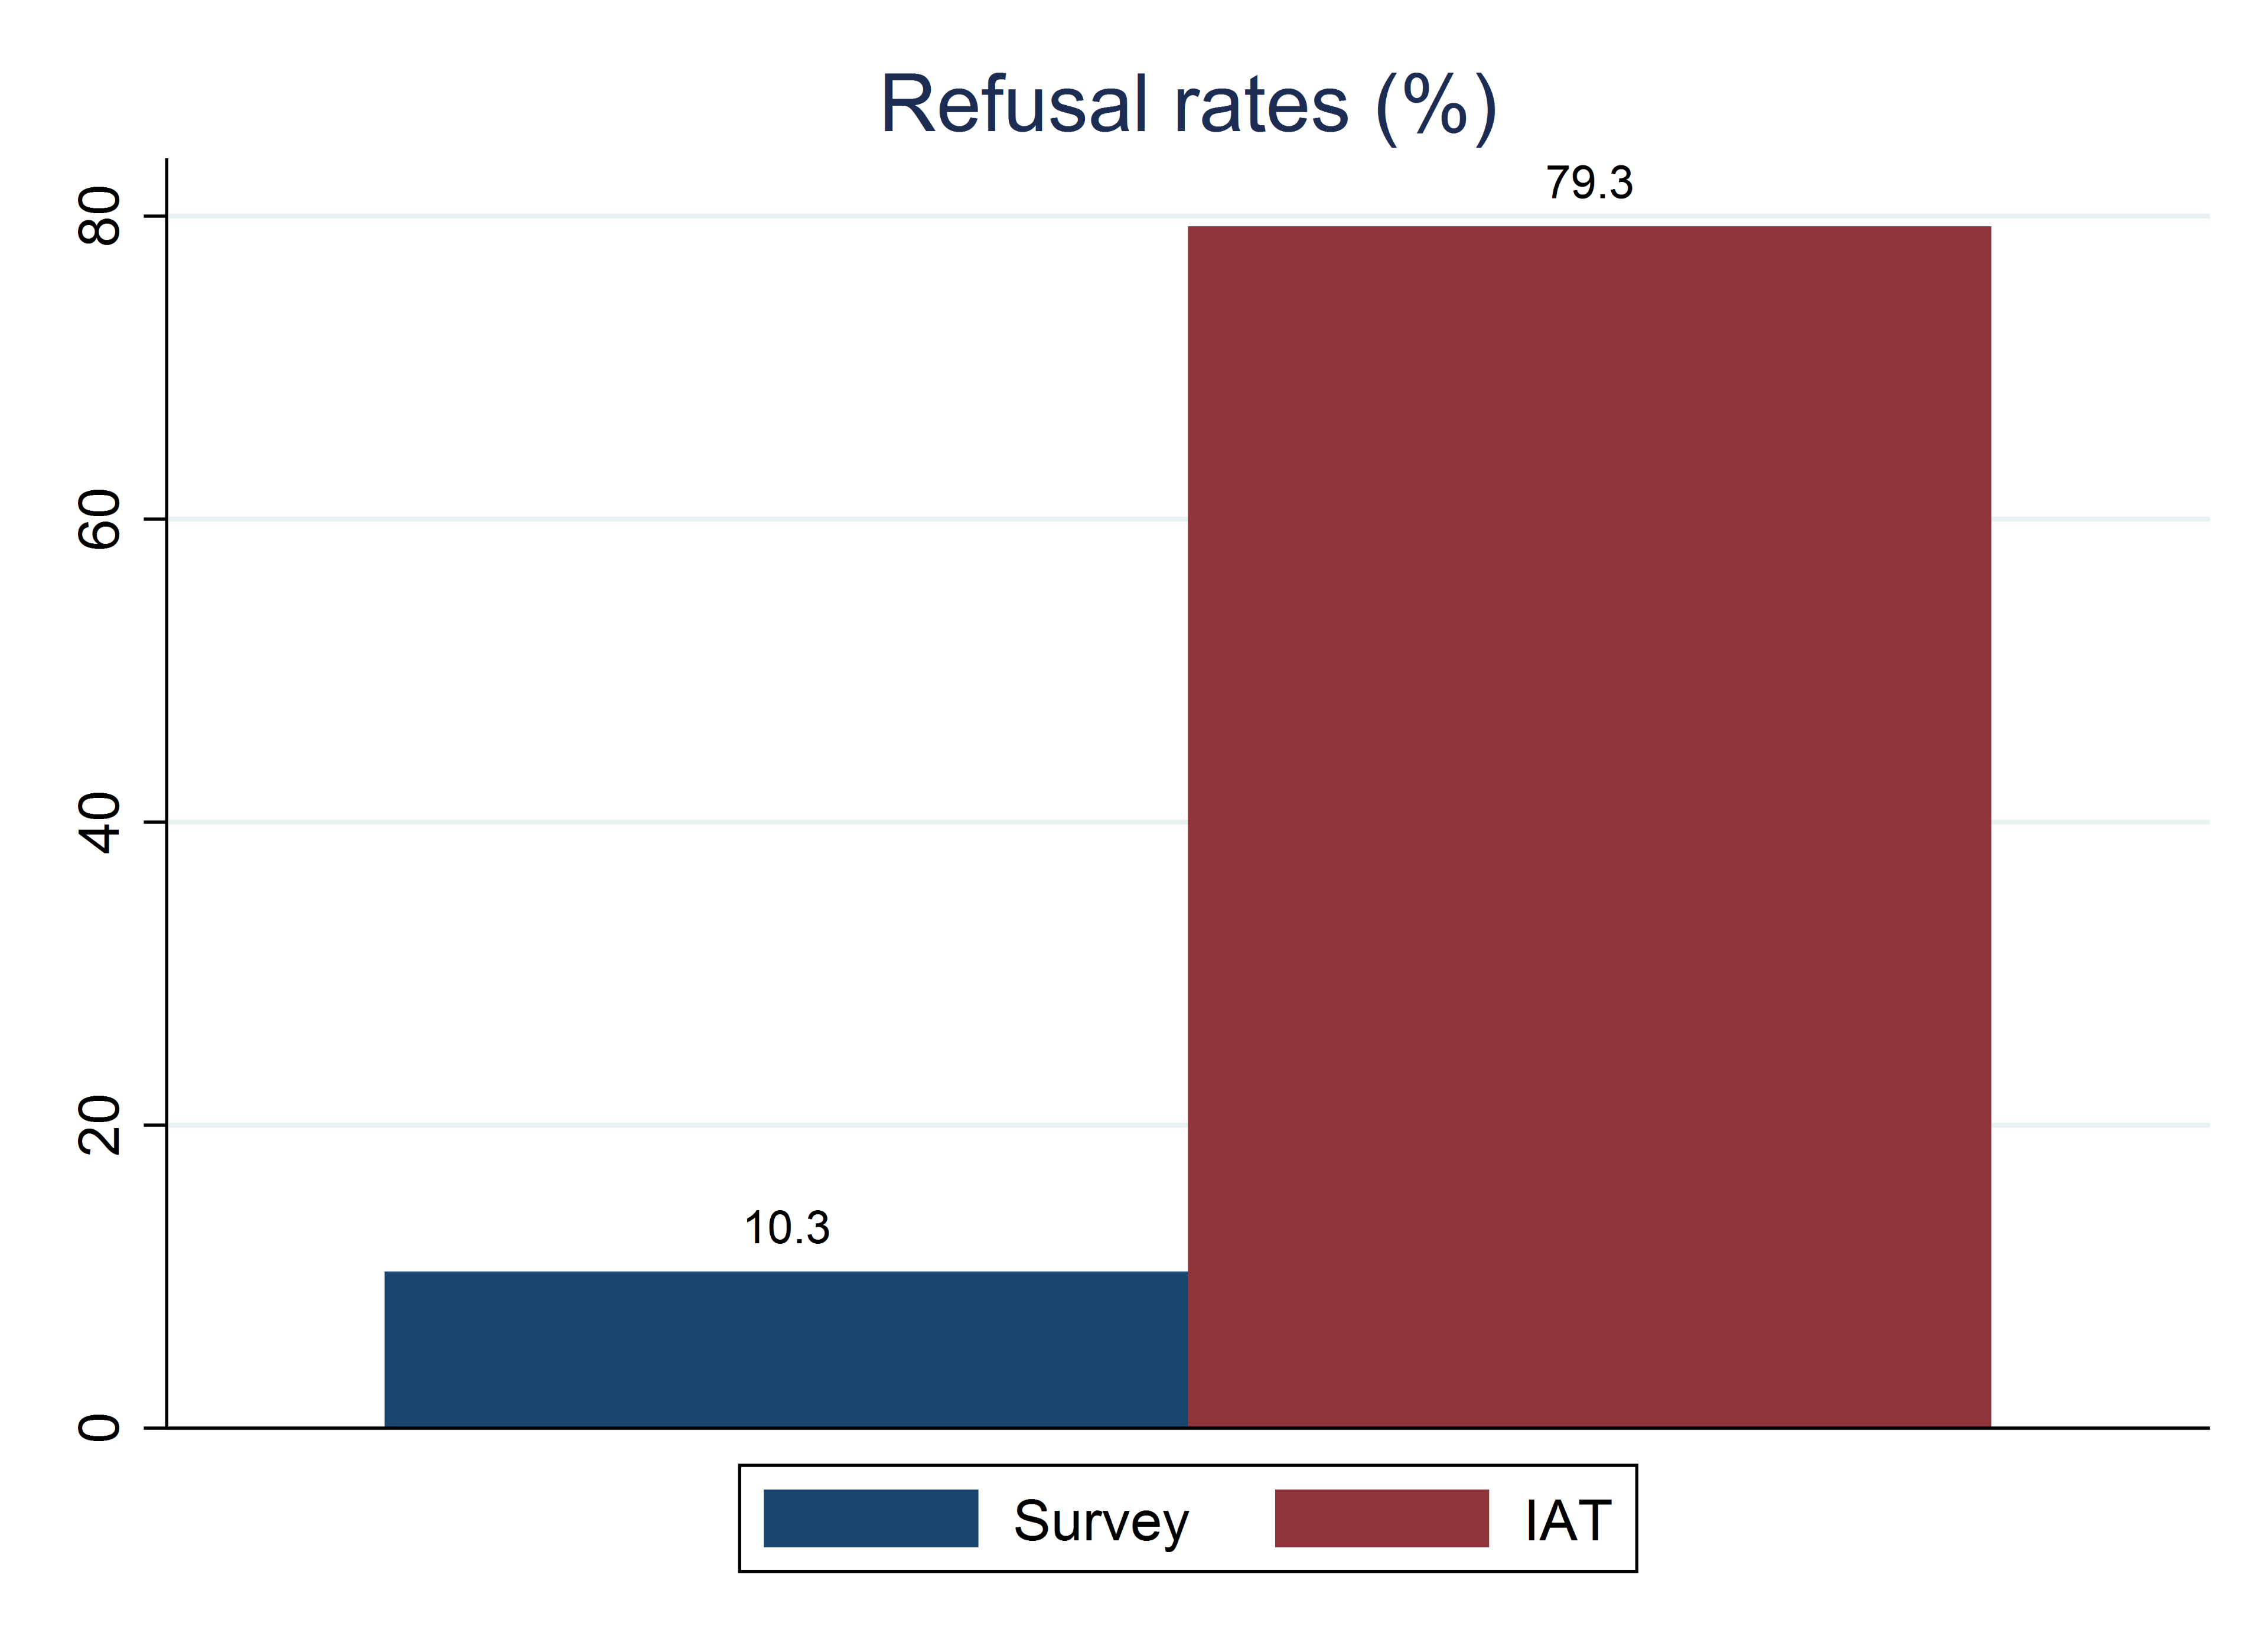
\includegraphics[width=0.49\textwidth,height=\textheight]{examples/quality-checks-fig1.png}
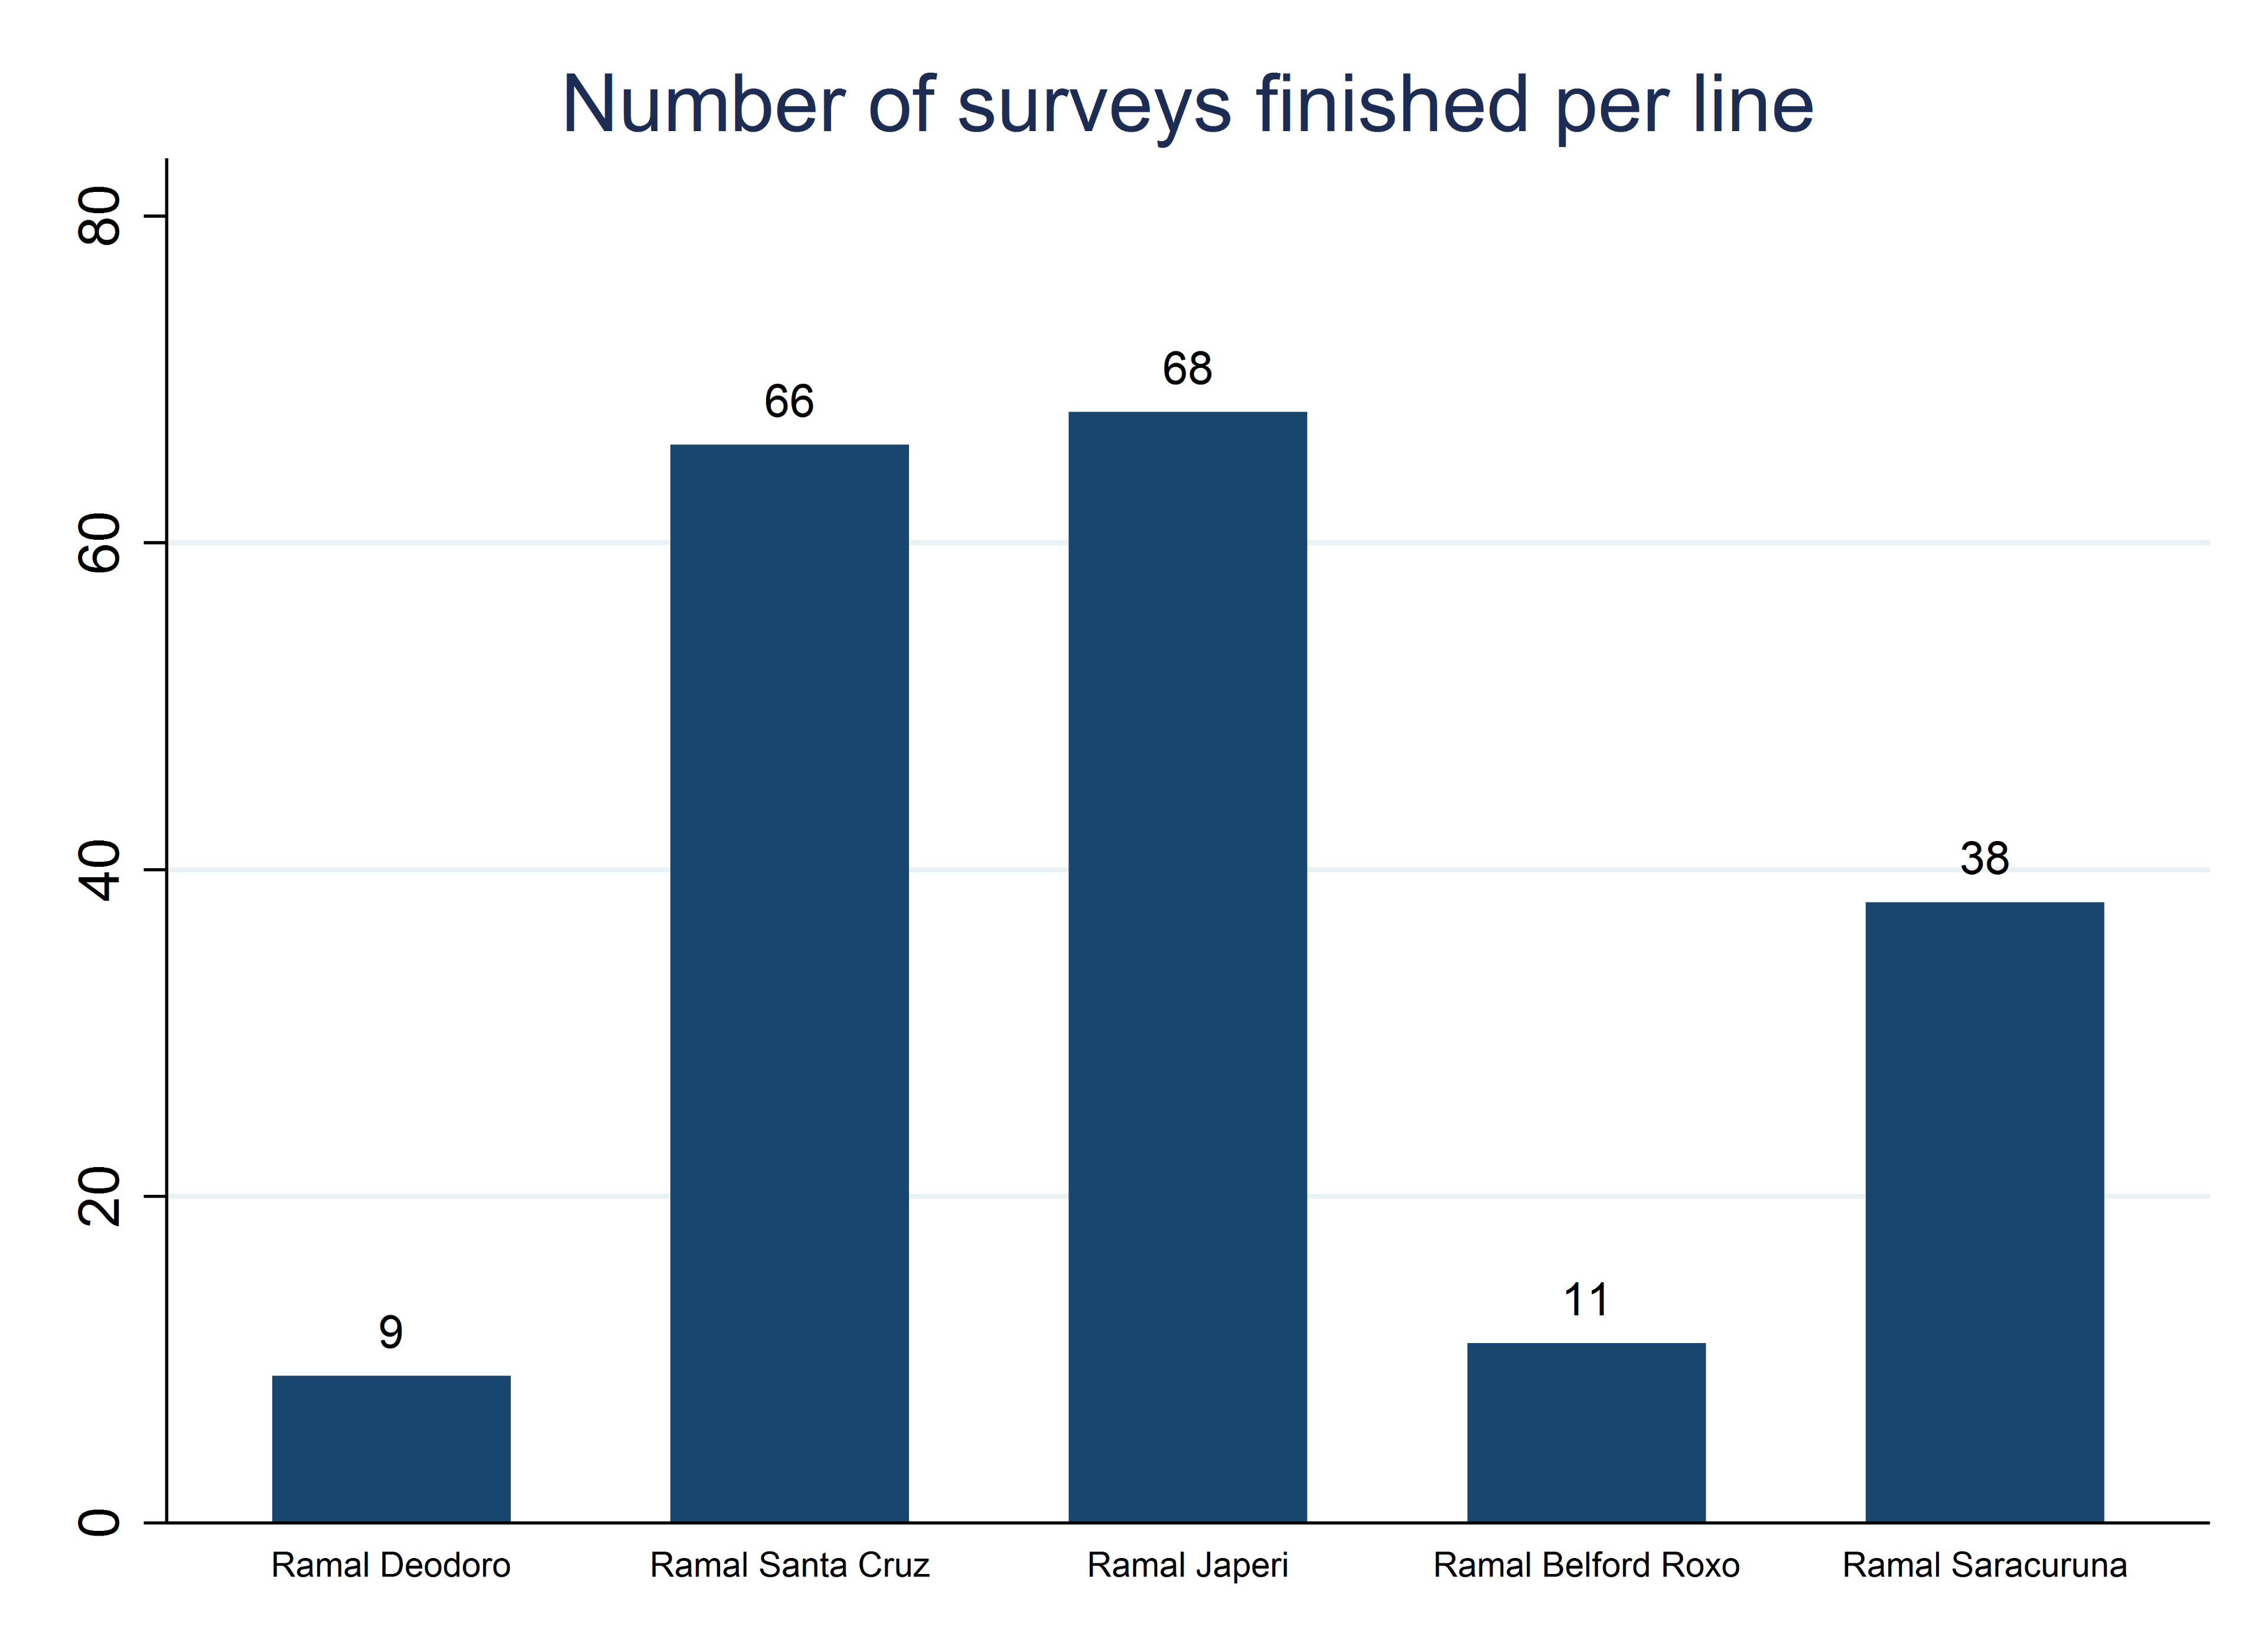
\includegraphics[width=0.49\textwidth,height=\textheight]{examples/quality-checks-fig2.png}
\end{ex}

\hypertarget{handling-data-securely}{%
\section*{Handling data securely}\label{handling-data-securely}}
\addcontentsline{toc}{section}{Handling data securely}

All confidential data must be handled in such a way that only people specifically
approved by an Institutional Review Board (IRB),
or specified in the Data Licensing Agreement (DLA),
are able to access the data.\index{institutional review board (IRB)}
Data can be confidential for multiple reasons;
two very common reasons are that the data contains
personally-identifying information (PII)\footnote{More details about what makes data PII and
  links to more resources on the extra consideration that
  must be taken when working with PII data
  can be found on the DIME Wiki:
  \url{https://dimewiki.worldbank.org/Personally_Identifiable_Information_(PII)}.}
\index{personally-identifying information}
or that the data owner has specified restricted access.\footnote{Read more about data security and the options you have to protect your data
  either on the DIME Wiki:
  \url{https://dimewiki.worldbank.org/Data_Security},
  or under Pillar 4 in the DIME Research Standards
  \url{https://github.com/worldbank/dime-standards}.}

\hypertarget{encrypting-data}{%
\subsection*{Encrypting data}\label{encrypting-data}}
\addcontentsline{toc}{subsection}{Encrypting data}

\textbf{Data encryption} is a group of tools and methods
to ensure that confidential files are unreadable and unusable
even if laptops are stolen, servers are hacked,
or unauthorized access to the data is obtained in any other way.\footnote{More details on what encryption is and
  how it should be used to protect your data
  can be found on the DIME Wiki:
  \url{https://dimewiki.worldbank.org/Encryption}.}\index{encryption}
Proper encryption is central to secure data handling,
and can rarely be condensed into a single tool or method,
as the data will travel through many servers, devices, and computers
from the source of the data to the final analysis.
Encryption should be seen as a system
that is only as secure as its weakest link.
This section recommends a streamlined encryption workflow,
so that it is easy as possible to make sure
the entire chain is easy to manage and is sufficiently secure.

All encryption relies on a password or encryption key
for both encrypting and decrypting information.
Encryption makes data files completely unusable
to anyone who obtains them if they do not have the specific decryption key.
This is a higher level of security than most password-protection,
because password-protected information is often readable
if the password is bypassed or the storage server is compromised.
You will need to share and store these keys carefully;
if you lose them or cannot match them to encrypted information,
the information is permanently lost.
Therefore, you should treat access to encryption keys
as equivalent to access to the confidential information.
It is never secure to share these passwords or keys by email,
WhatsApp or other common modes of communication;
instead, use a secure password manager built for this purpose.\footnote{Read our step-by-step guide for how to get started with password managers
  under Pillar 4 in the DIME Research Standards:
  \url{https://github.com/worldbank/dime-standards}.}

There are two contexts for encryption you should be aware of.
\textbf{Encryption-in-transit} protects your data
when it is sent over the internet.\footnote{More details on what encryption-in-transit is and
  when it should be used to protect your data
  can be found on the DIME Wiki:
  \url{https://dimewiki.worldbank.org/Encryption\#Encryption_in_Transit}.}
This is a standard, passive protection that almost all internet-based services use;
you only need to worry about it if you are creating a custom transfer solution.
\textbf{Encryption-at-rest} protects your data
when it is stored on a server, computer, or drive.\footnote{More details on what encryption-at-rest is and
  when it should be used to protect your data
  can be found on the DIME Wiki:
  \url{https://dimewiki.worldbank.org/Encryption\#Encryption_at_Rest}.}

There are two main types of encryption algorithms and they are called
\textbf{symmetric encryption}\footnote{More details on what symmetric encryption is and
  when it should be used can be found on the DIME Wiki:
  \url{https://dimewiki.worldbank.org/Encryption\#Symmetric_Encryption}.}
and \textbf{asymmetric encryption}\footnote{More details on what asymmetric encryption is and
  when it should be used can be found on the DIME Wiki:
  \url{https://dimewiki.worldbank.org/Encryption\#Asymmetric_Encryption}.}.
In symmetric encryption,
the same key is used to both encrypt and decrypt the data.
In asymmetric encryption, one key is used to encrypt data,
and another key from the same ``pair'' is used to decrypt it.
You, as a user, need to keep track of these keys.
While encryption keys for asymmetric encryption are often
automatically provided to the devices recording or inputting information,
only people listed on your IRB should have access to decryption keys
or symmetric-encryption keys.

Typically, unless you have access to an approved
enterprise version of data sharing software,
you will need to set up encryption at rest for your data
in two locations --
server or web storage during data acquisition and local storage afterwards.
You should never trust that this is automatically implemented
unless a cybersecurity expert within your organization
has specified that a specific service is appropriate to your use case.
In all other cases you should follow the steps laid out in this section,
where you set up your own encryption
where you, and only you, are in full control of who has access to the key.

\hypertarget{collecting-and-storing-data-securely}{%
\subsection*{Collecting and storing data securely}\label{collecting-and-storing-data-securely}}
\addcontentsline{toc}{subsection}{Collecting and storing data securely}

Most data collection software will automatically encrypt
all data in transit (i.e., upload from field or download from server).
However, it is necessary to ensure that confidential data
are protected when stored on a server
owned by the data collection software provider
or which can be accessed by people not on your research team
(including your local IT or system administrators).
In most data collection platforms,
encryption-at-rest needs to be explicitly enabled and operated by the user.
When collecting data, the tablets or the browsers used for data collection
should encrypt all information before submitting it to the server,
and you should decrypt it only after downloading to your local machine.

This is a perfect use case for \textbf{asymmetric encryption}
where there are two keys, forming a ``public/private key pair''.
The public key can safely be sent to all tablets or browsers
so it can be used for encrypting the data before it is submitted to the server.
Only the private key in the same key pair can then be used to decrypt that data
so it can be accessed after it has been received.
The private key should be kept secret and
should not be shared with anyone not listed on the IRB.
Again, you must store the key pair in a secure location,
such as a secure note in a password manager,
as there is no way to access your data if the private key is lost.
If your data collection service allows you to browse data in the browser,
then the encryption is only implemented correctly if you are asked for the key each time.

The data security standards that apply
when receiving confidential data from the field
also apply when transferring confidential data to the field,
such as sampling or enumeration lists containing PII.\index{data transfer}
In some survey software,
you can use the same encryption that allows you to receive data securely
from the field, to also send confidential data,
such as an identifying list of respondents, to the field.
Otherwise, you will need to create a securely stored file,
transfer it to the field team using an insecure tool,
and have them decrypt the information locally
using a key that is transferred using a secure password manager.
This process will be more similar to that for securely `storing\} data,
which we discuss next.

The first thing you need to do before planning how to securely send or receive data,
is to plan how to securely store data after it has been transferred.
Typically, you want to store your data so that you can decrypt and access it,
interact with it and then encrypt it again.
(Usually, you will not want to \emph{edit} this data,
but only extract non-sensitive pieces of it to an insecure location.)
That is a perfect use case for \textbf{symmetric encryption}
where the same key is used to both encrypt and decrypt your files.\index{symmetric encryption}
Think of this type of encryption similarly to a physical safe,
where you have one key which is used to both add and access contents.

The equivalent to the safe in secure data storage is an encrypted folder,
which you can set up using, for example, VeraCrypt.
You can interact with files in an encrypted folder,
and modify them like any unencrypted file,
if and only if you have the key.
This is an implementation of encryption-at-rest.
There is absolutely no way to restore the data if you lose your key,
so we cannot stress enough the importance of using a password manager,
or equally secure solution, to store these encryption keys.

It is becoming more and more common that development research
is done on data set that is too big to store on a regular computer,
and instead the data is stored and processed in a cloud environment.
There are many available cloud storage solutions
and you need to understand how the data is encrypted and how the keys are handled.
This is likely another case where a regular research team will have to ask a cybersecurity expert.
After someone have helped you to set up a secure cloud storage,
if you were to download a sample of the data --
for example to develop your code on --
then you need to remember to encrypt the data when stored on your computer.

\hypertarget{backing-up-original-data}{%
\subsection*{Backing up original data}\label{backing-up-original-data}}
\addcontentsline{toc}{subsection}{Backing up original data}

In addition to encrypting your data, you must protect it
from being accidentally overwritten or deleted.
This is done through a back-up protocol,
which creates additional copies of your original data,
exactly as received and finalized,
in secure locations that will remain permanently available
but are not intended for frequent access.
Here is an example of such a protocol:

\begin{enumerate}
\def\labelenumi{\arabic{enumi}.}
\item
  Create an encrypted folder in your project folder.
  This should be on your computer, and could be in a shared folder.
\item
  Download your original data from your data source to that encrypted folder.
  If your data source is a survey and the data was encrypted during data collection,
  then you will need \emph{both} the private key used during data collection to be able to download the data,
  \emph{and} the key used when you created the encrypted folder to save it there.
  This your first copy of your raw data, and the copy you will use for cleaning and analysis.
\item
  Create a second encrypted folder on an external drive that you can keep in a secure location.
  Copy the data you just downloaded to this second encrypted folder.
  This is the ``master" backup copy of the raw data.
  You should never work with this data on a day-to-day basis.
  You should not use the same encrypted folder or the same key as above,
  because if you use the same key and lose the key,
  then you will have lost access to both encrypted folders.
  If you have a physical safe where you can securely store the external drive,
  then you do not need to encrypt the data
  and thereby do not risk losing access by losing an encryption key.
\item
  Finally, create a third encrypted folder.
  Either you can create this on your computer and upload it to a long-term cloud storage service (not a sync software),
  or you can create it on another external hard drive or computer that you then store in a second location,
  for example, at another office of your organization.
  This is the \texttt{golden\ master"\ backup\ copy\ of\ the\ raw\ data.\ You\ should\ never\ store\ the}golden master" copy in a synced folder,
  as it would be deleted in the cloud storage if it is deleted on your computer.
  You should also never work with this data;
  it exists only for recovery purposes.
\end{enumerate}

This handling satisfies the \textbf{3-2-1 rule}:
there are two on-site copies of the data and one off-site copy,
so the data can never be lost in case of hardware failure.
If you remain lucky, you will never have to access your ``master'' or ``golden master'' copies --
you just want to know it is there, safe, if you one day end up needing it.

\hypertarget{looking-ahead-4}{%
\section*{Looking ahead}\label{looking-ahead-4}}
\addcontentsline{toc}{section}{Looking ahead}

This chapter provided a road map to the acquisition of original data.
It outlined guidelines for ensuring that you have effective ownership
or licensing of data that you obtain or collect,
and how to make those materials available in the future.
It also provided an extensive guide for one of the most common --
and challenging --
methods of data collection: primary electronic surveys.
Finally, it emphasized the secure handling of this potentially sensitive information,
giving you a range of tools and a complete workflow
for transferring and storing data securely at all times.
Once your original data is completely transferred, securely stored, and backed up,
the data acquisition stage is complete, as
summarized in the figure accompanying this chapter.
This is when the heavy lifting with statistical software starts.
Before you can proceed to analyze your data
and answer your project's research questions,
you first need to check the quality of the data acquired,
make sure you have the right information in the right format, and prepare it for analysis.
This process, which we call data cleaning and processing,
is described in the next chapter.

\begin{figure}
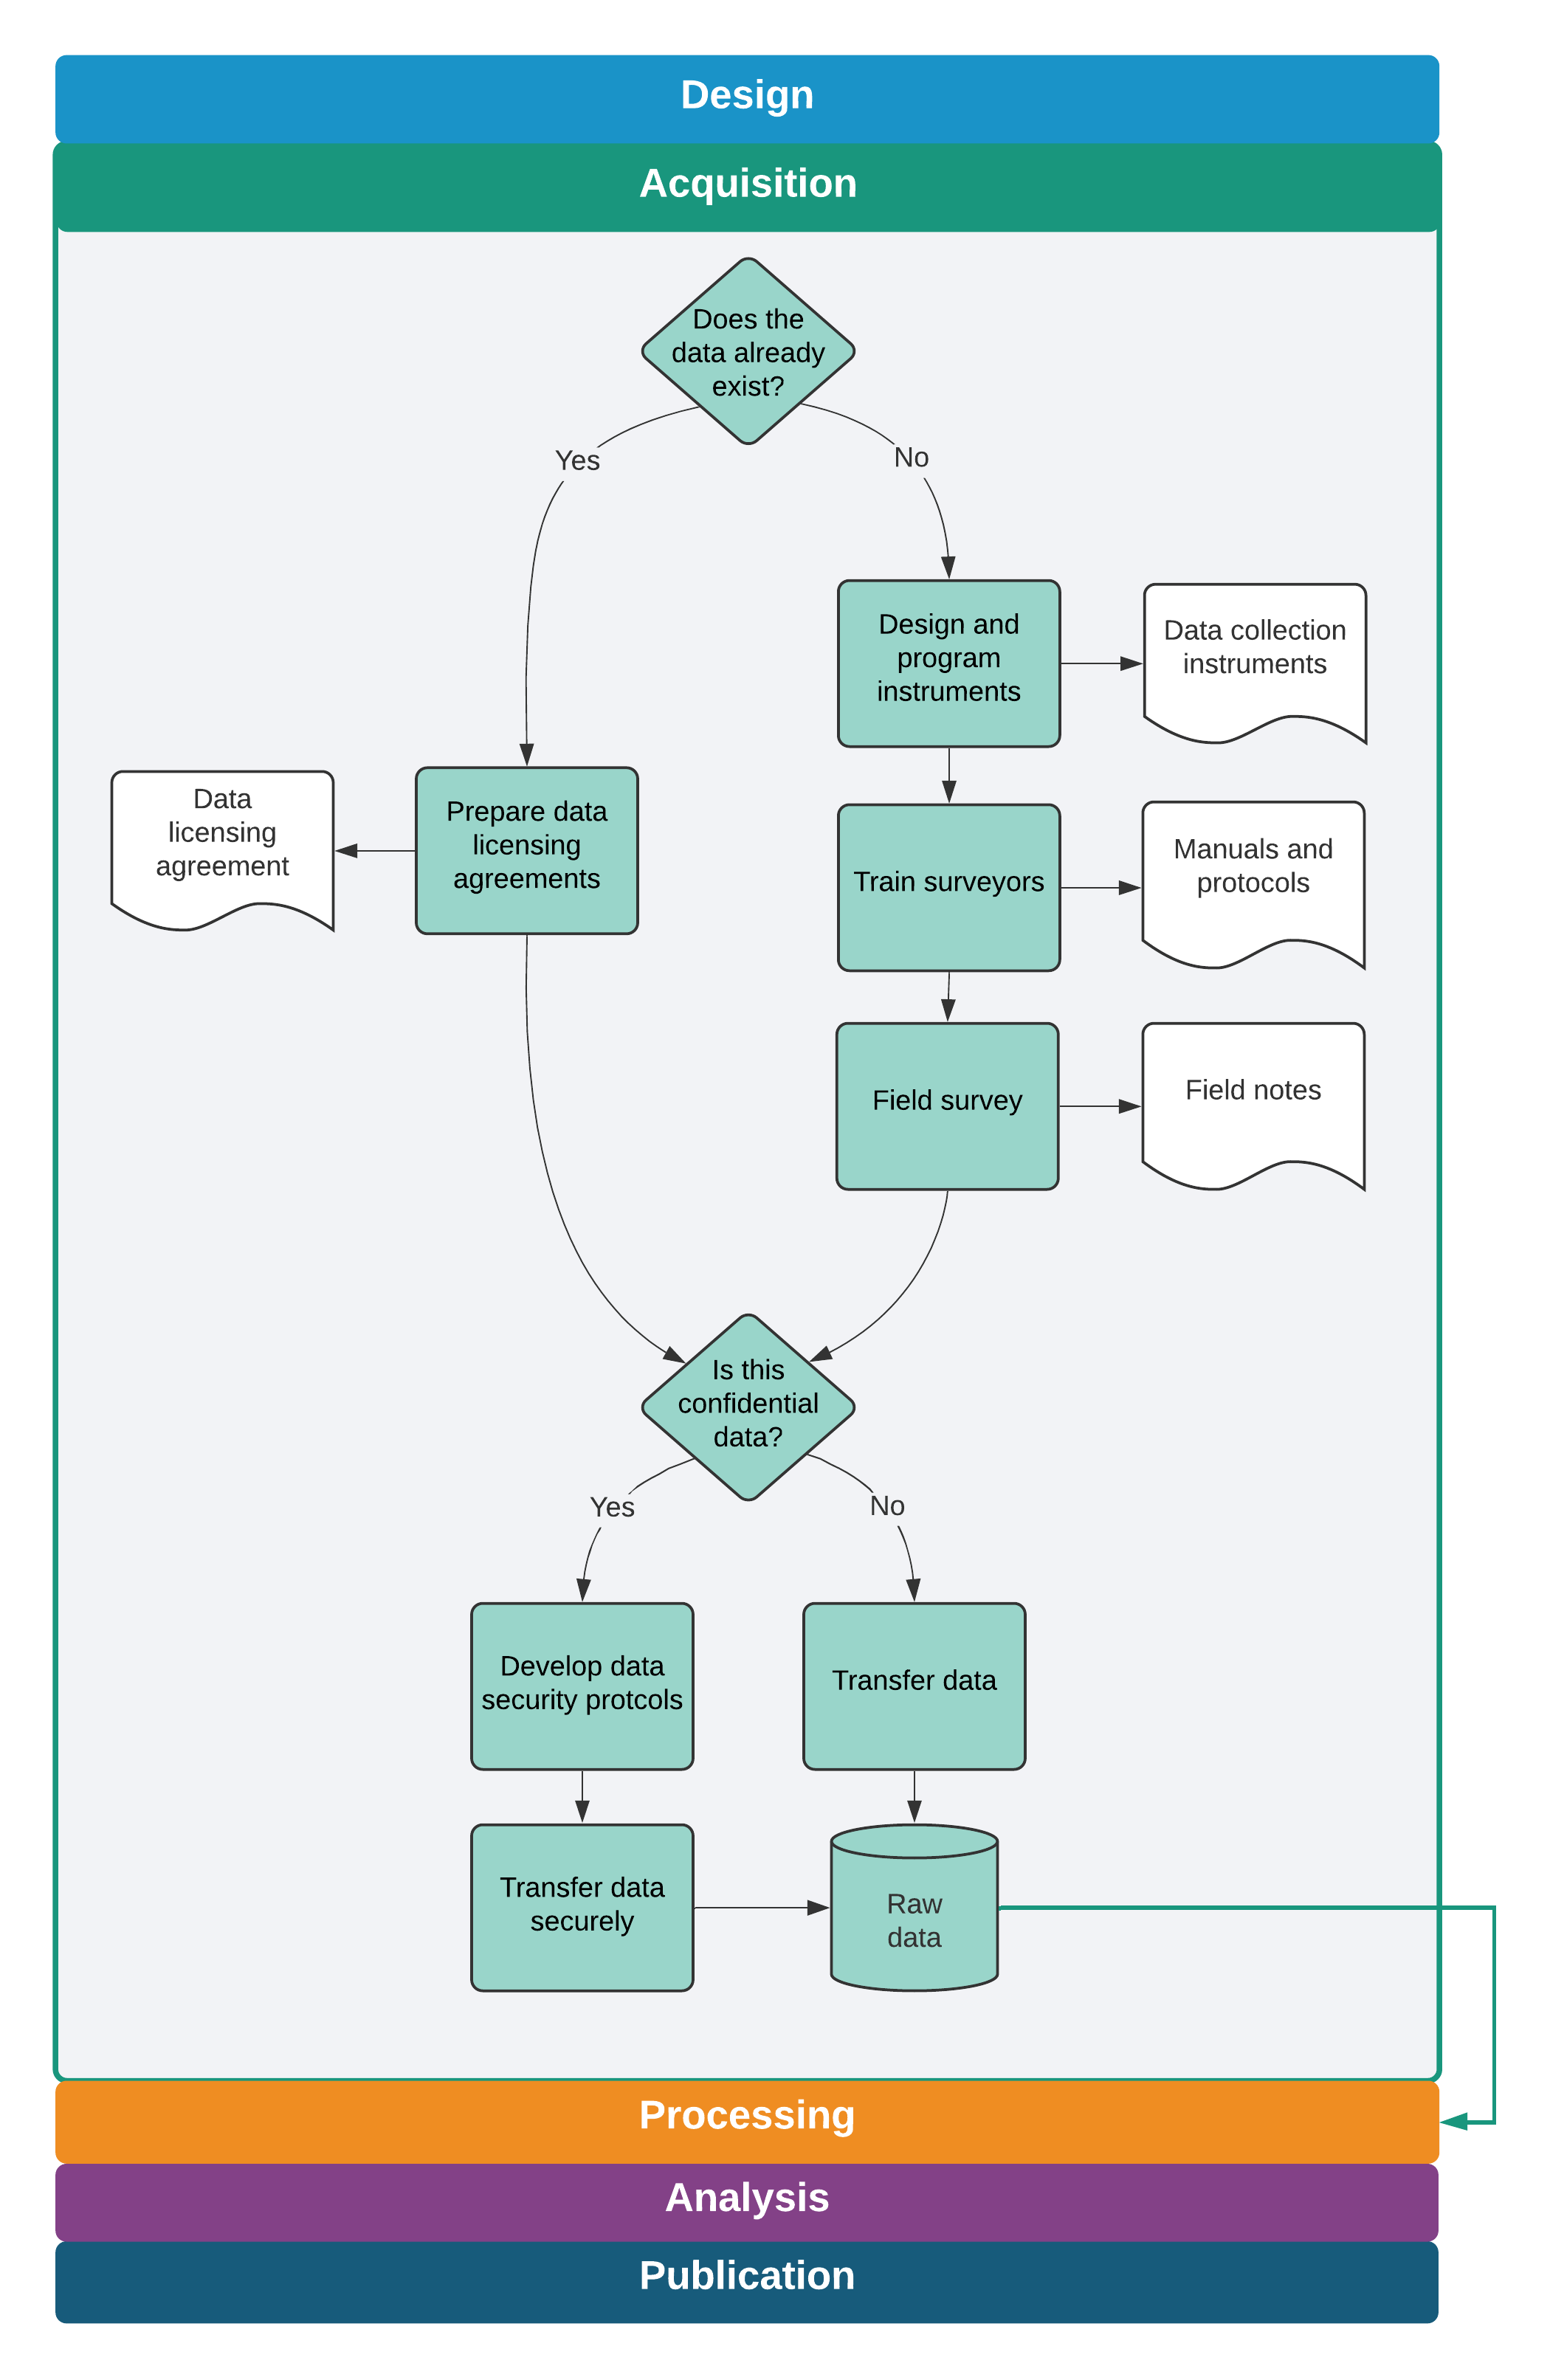
\includegraphics[width=29.17in]{diagrams/Acquisition} \caption{Data acquisition tasks and outputs}\label{fig:unnamed-chunk-26}
\end{figure}

\hypertarget{processing}{%
\chapter{Cleaning and processing research data}\label{processing}}

Original data comes in a variety of formats,
most of which are not immediately suited for analysis.
The process of preparing data for analysis has many different names:
data cleaning, data munging, data wrangling.
But they all mean the same thing --
transforming raw data into a convenient format for your intended use.
This is the most time-consuming step of a project's data work,
particularly when primary data is involved;
it is also essential for data quality.
A structured workflow for preparing newly-acquired data for analysis
is essential for efficient, transparent, and reproducible data work.
One key point of this chapter is that no changes are made to the contents of data at this point.
We consider creating new variables, imputing values and correcting outliers
to be research decisions, and will discuss those in the next chapter.
Therefore, the clean dataset,
which is the main output from the workflow discussed in this chapter,
contains the same information as the raw data,
but in a format that is ready for use with statistical software.

This chapter describes the various tasks involved in making newly-acquired data ready for analysis.
The first section teaches you how to make your data \emph{tidy}.
This means adjusting how the dataset is organized
until the relationship between rows and columns is well-defined.
The second section describes quality assurance checks,
which are necessary to verify data accuracy.
The third section covers de-identification,
as removing direct identifiers early in the data handling process helps to ensure privacy.
The final section discusses how to examine each variable in your dataset and
make sure that it is as well documented and as easy to use as possible.
Each of these tasks is implemented through code,
and resulting datasets can be reproduced exactly by running this code.
The raw data files are kept exactly as they were acquired,
and no changes are made directly to them.

\begin{summary}
\hypertarget{summary-cleaning-and-processing-research-data}{%
\subsection*{Summary: Cleaning and processing research data}\label{summary-cleaning-and-processing-research-data}}
\addcontentsline{toc}{subsection}{Summary: Cleaning and processing research data}

After data is acquired, it must be structured for analysis in accordance with the research design, as laid out in the data linkage tables and the data flowcharts discussed in Chapter \ref{measurement}. Data processing requires first transforming the unprocessed materials from partners or data collection into the appropriate tables and units of observation, then producing clean data sets that match the ground truth observations. To do this, you will:

\textbf{1. Tidy the data.} Many raw datasets as received will not have an unambiguous identifier, and the rows in the dataset often will not match the units of observation specified by the research plan and data linkage table. To prepare the data for analysis, you must:

\begin{itemize}
\tightlist
\item
  Determine the \emph{unique identifier} for each unit of observation that you require.
\item
  Transform the raw data so that the desired \emph{unit of observation} uniquely identifies rows in each dataset.
\end{itemize}

\textbf{2. Validate data quality.} Data completeness and quality should be validated upon receipt to ensure the data is an accurate representation of the characteristics and individuals it is supposed to contain. This includes:

\begin{itemize}
\tightlist
\item
  Checking that the data is \emph{complete}, that is, that all the expected observations were received and validated them against the sample.
\item
  Making sure data points are \emph{consistent} across variables and datasets.
\item
  Exploring the \emph{distributions} of key variables to identify outliers and other unexpected patterns.
\end{itemize}

\textbf{3. De-identify, clean, and prepare the data.} You should archive and/or publish the raw data after processing and de-identifying. Before publication, you should ensure that the processed version is highly accurate and appropriately protects the privacy of individuals, by doing the following:

\begin{itemize}
\tightlist
\item
  \emph{De-identifying the data}, in accordance with best practices and relevant privacy regulations.
\item
  \emph{Correcting data points} which are identified as being in error compared to ground reality.
\item
  \emph{Recoding, documenting, and annotating datasets} so that all dataset contents are fully interpretable by future users, whether or not they were involved in the acquisition process.
\end{itemize}

\hypertarget{takeaways-4}{%
\subsubsection*{Takeaways}\label{takeaways-4}}
\addcontentsline{toc}{subsubsection}{Takeaways}

\textbf{TTLs/PIs will:}

\begin{itemize}
\tightlist
\item
  Indicate the units of observation that are needed for experimental design and supervise development of appropriate unique identifiers
\item
  Indicate priorities for quality checks, including key indicators and reference values
\item
  Provide guidance on how to resolve all issues identified in data processing, cleaning and preparation
\item
  Publish and/or archive the prepared dataset
\end{itemize}

\textbf{RAs will: }

\begin{itemize}
\tightlist
\item
  Develop code, data, and documentation linking datasets with data map and study design, and tidy all datasets to correspond to the required units of observation
\item
  Manage data quality checks, clearly communicate issues to TTL/PI, data producers, and/or field teams
\item
  Implement data cleaning processes; generate and maintain detailed documentation
\item
  Prepare dataset for publication by de-identifying, correcting field errors, and preparing documentation
\end{itemize}

\hypertarget{key-resources-4}{%
\subsubsection*{Key Resources}\label{key-resources-4}}
\addcontentsline{toc}{subsubsection}{Key Resources}

\begin{itemize}
\tightlist
\item
  \textbf{iefieldkit stata package}: suite of commands to enable reproducible data cleaning and processing.

  \begin{itemize}
  \tightlist
  \item
    Explanation: \url{https://dimewiki.worldbank.org/Iefieldkit}.
  \item
    Code: \url{https://github.com/worldbank/iefieldkit}.
  \end{itemize}
\item
  \textbf{ietoolkit stata package}: suite of commands to enable reproducible data management and analysis.

  \begin{itemize}
  \tightlist
  \item
    Explanation: \url{https://dimewiki.worldbank.org/Ietoolkit}.
  \item
    Code: \url{https://github.com/worldbank/ietoolkit}.
  \end{itemize}
\item
  *\textbf{DIME Analytics Continuing Education Session on Tidying Data}: \url{https://osf.io/p4e8u/}
\item
  \textbf{De-identification article on DIME Wiki}: \url{https://dimewiki.worldbank.org/De-identification}
\end{itemize}
\end{summary}

\hypertarget{making-data-tidy}{%
\section*{Making data ``tidy''}\label{making-data-tidy}}
\addcontentsline{toc}{section}{Making data ``tidy''}

The very first step in creating an analysis-friendly dataset
is understanding the data acquired,
and using this understanding to translate the data into an intuitive format.
This section discusses what steps may be needed to make sure that each row
in your \textbf{data tables}\footnote{\textbf{Data table:}
  data that is structured into rows and columns.
  Also called \emph{tabular datasets} or \emph{rectangular data}.
  Examples of non-rectangular data are written text,
  NoSQL and graph databases, or files such as images.}
represents one observation.
Getting to such a format may be harder than expected,
and the \textbf{unit of observation}\footnote{\textbf{Unit of observation:}
  the unit described by the data. In datasets, it is ideally what each row represents.
  More details on the concept of unit of observations
  can be found on the DIME Wiki:
  \url{https://dimewiki.worldbank.org/Unit_of_Observation}.}\index{unit of observation}
may be ambiguous in many raw datasets.
This section will present what we call a \emph{tidy} data format,
which is, in our experience, the ideal format to handle tabular data.
We will treat tidying data as the first step in data cleaning even though, in practice,
both tidying and quality monitoring should be done simultaneously as data is received.
This is because quality assurance can only be finalized using tidied data,
when it is guaranteed that each observation is uniquely identified.

\hypertarget{establishing-a-unique-identifier}{%
\subsection*{Establishing a unique identifier}\label{establishing-a-unique-identifier}}
\addcontentsline{toc}{subsection}{Establishing a unique identifier}

An important step before starting to tidy a dataset is
to understand the \textbf{unit of observation}
and find out which variable or set of variables
is the \textbf{unique identifier} for each observation.\footnote{More details on the properties required for variables
  that uniquely identifies each observation
  can be found on the DIME Wiki:
  \url{https://dimewiki.worldbank.org/ID_Variable_Properties}.}\index{unique identifier}
As discussed in Chapter \ref{measurement},
the unique identifier will be used to link observations in this dataset
to data in other data sources according to the \textbf{data linkage table},\footnote{More details on DIME's data linkage table template
  and an example can be found on the DIME Wiki:
  \url{https://dimewiki.worldbank.org/Data_Linkage_Table}.}\index{data linkage table}
and the unique identifier for all observations
must be listed in the \textbf{master dataset}.\footnote{More details on DIME's master dataset template
  and an example can be found on the DIME Wiki:
  \url{https://dimewiki.worldbank.org/Master_Data_Set}.}\index{master dataset}
Ensuring that observations are uniquely and fully identified
is arguably the most important step in data cleaning.
It may be the case that the variables expected to uniquely identify
the raw data contain either missing or duplicate values.\footnote{We use the expression \textbf{raw data}
  to refer to the ``data in the state it was originally received by the research team''.
  In other sources, you will also see it used to refer to the
  ``corrected and compiled dataset created from received information,
  reflecting only that information'',
  which we call \textbf{clean data}.
  This applies to data acquired from partners as well as
  original data collected by the research team.}

It is also possible for a raw dataset to not include an unique identifier,
or that the identifier is not a suitable \textbf{project ID}.\footnote{More details on what makes an ID variable
  a suitable Project ID variable
  can be found on the DIME Wiki:
  \url{https://dimewiki.worldbank.org/ID_Variable_Properties\#Project_ID}.}
Suitable project IDs should, for example, not involve long strings
that are difficult to work with, such as a name,
or be an ID that is known outside the research team.
In such cases, cleaning begins by
adding a project ID to the raw data.
If a project ID already exists,
for this unit of observation,
then you should carefully merge it
from the master dataset
to the raw data
using other identifying information.\footnote{Such
  operations are commonly called `\texttt{merges"\ in\ Stata,\ and\ \ \ \ \ "joins"\ in\ R\textquotesingle{}s}tidyverse\texttt{dialect.\ \ \ \ \ We\ will\ use\ the\ term}merge` in this book.}
If a project ID does not exist,
then you need to generate one,
add it to the master dataset,
and then merge it back into the raw data.
Note that while digital survey tools create
unique identifiers for each data submission,
that is not the same as having a unique ID variable
for each observation in the sample,
as there can be multiple submissions
for the same observation.

DIME Analytics created an automated workflow to identify, correct and document
occurrences of duplicated entries in the unique identifier using
\texttt{ieduplicates} and \texttt{iecompdup},\index{ieduplicates}\index{iecompdup}
two Stata commands included in the \texttt{iefieldkit} package\index{iefieldkit}.
One advantage of using \texttt{ieduplicates}\footnote{Read more about how to install and use \texttt{ieduplicates} and
  how the command can help you efficiently deal with duplicates
  on the DIME Wiki:
  \url{https://dimewiki.worldbank.org/ieduplicates}.}
to correct duplicated entries is that it creates \emph{duplicates reports}
which records each corrections made and documents the reason for it.
Even if you are not using this command,
it is important to keep a record of all cases of duplicated IDs encountered
and how they were resolved.

\begin{ex}
\hypertarget{demand-for-safe-spaces-case-study-establishing-a-unique-identifier}{%
\subsection{Demand for Safe Spaces Case Study: Establishing a Unique Identifier}\label{demand-for-safe-spaces-case-study-establishing-a-unique-identifier}}

All datasets have a ``unit of observation'', and the first columns of each dataset should uniquely identify which unit is being observed. In the \emph{Demand for Safe Spaces} project, as in all projects, the first few lines of code that import each raw dataset immediately ensure that this is true and apply any corrections from the field needed to fix errors with uniqueness.

The code segment below imports the crowdsourced ride data and uses the \texttt{ieduplicates} command to remove duplicate values of the uniquely identifying variable in the dataset. The corresponding filled \texttt{ieduplicates} form included below shows how the command generates information documenting and resolving duplicated IDs in data collection. After applying the corrections, the code confirms that the data is uniquely identified by riders and ride IDs and saves it in an optimized format.

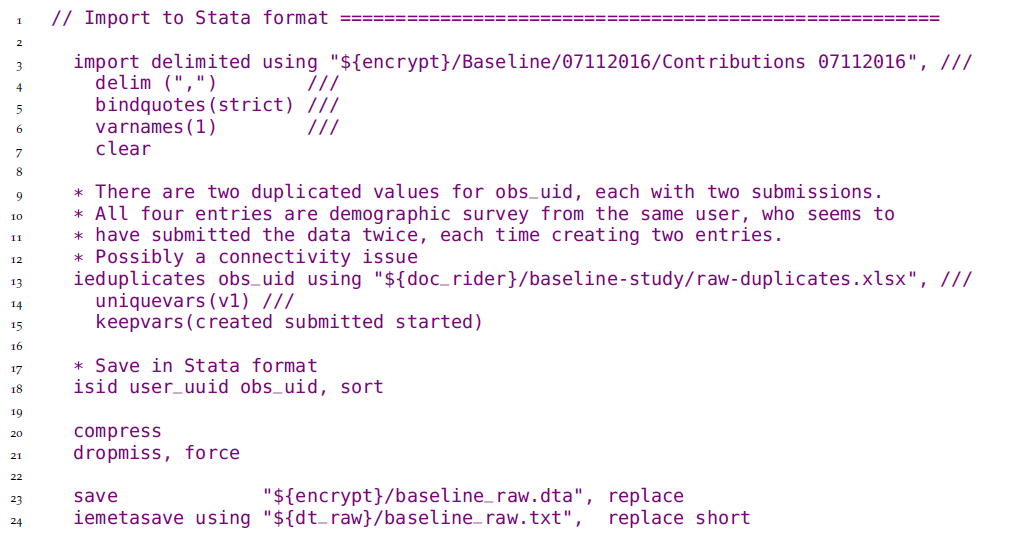
\includegraphics{examples/ch5-establishing-a-unique-identifier.png}

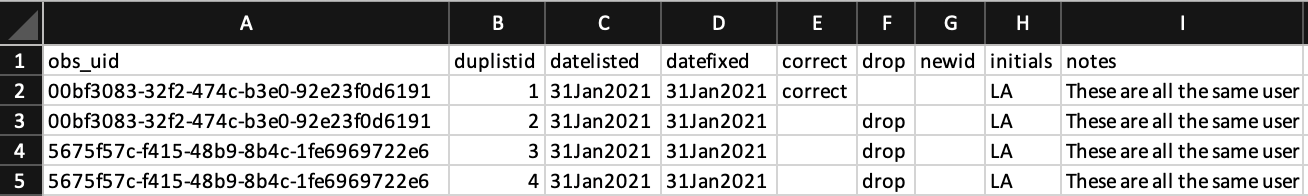
\includegraphics{examples/duplicates-report-filled.PNG}

\begin{quote}
The complete do-file can be found at \url{https://git.io/Jtgml}.
\end{quote}
\end{ex}

\hypertarget{tidying-raw-data}{%
\subsection*{Tidying raw data}\label{tidying-raw-data}}
\addcontentsline{toc}{subsection}{Tidying raw data}

Though raw data can be acquired in all shapes and sizes,
it is most commonly received as one or multiple data tables.
These data tables can organize information in multiple ways,
and not all of them result in easy-to-handle datasets.
Fortunately, a vast literature of database management has identified the format
that makes interacting with the data as easy as it can be.
We call data in such format \textbf{tidy}.
A data table is tidy when each column represents one \textbf{variable},\footnote{\textbf{Variable:} the collection of all data points
  that measure the same attribute for each observation.}
each row represents one observation,
and all variables in it have the same unit of observation.
Every other format is \emph{untidy}.
This may seem trivial, but raw data,
and raw survey data in particular,
is rarely received in a tidy format.

The most common case of untidy raw data encountered in development research
is a dataset with multiple units of observations stored in the same data table.
Take, for example, a household survey that includes household-level questions,
as well as a household member roster.
Such raw datasets usually consists of a single data table
where questions from the household member roster are saved in different columns,
one for each member, with a corresponding member suffix,
and household-level questions are represented by one column each.
When your rows include multiple nested observational units,
then the identifying variable does not identify all observations on that row,
as there is more than one unit of observation on the same row.

Survey data containing nested units of observation is typically
imported from survey platforms in \textbf{wide format}.\footnote{\textbf{Wide data:}
  a data table where a single variable is divided into multiple columns,
  for example one for each individual in a household.}\index{wide data format}
Wide format data could have, for instance,
one column for a household-level variable (for example \texttt{ownsfridge}),
and a few columns for household member-level variables (for example \texttt{sex\_1}, \texttt{sex\_2}).
Raw data is often saved in this format because it's the most efficient way to transfer it:
adding different levels of observation into the same data table
allows for data to be transferred in a single file.
However, this leads to the widespread practice of interacting with data in wide format,
although doing so is often inefficient and error-prone.

To understand how dealing with wide data can be complicated,
imagine you need to calculate the share of women
in each household using the household level data described above.
In a wide data table you will either have to first create variables counting
the number of women and the total number of household members,
and then calculate the share,
or you will have to transform the data to a different format.
In a tidy data table, however, where each row is a household member,
you can easily aggregate the share of women by household,
without additional steps,
and then merge the result to the household-level data tables.
Tidy data tables are also easier to clean,
as each attribute only needs to be checked once,
and each column corresponds directly to one question in the questionnaire.
Finally, as you will see in Chapter \ref{analysis},
summary statistics and distributions are much simpler
to generate from tidy data tables.

As mentioned earlier, there are unlimited ways for data to be untidy;
wide format is only one of those ways.
Another example is a data table containing both information on transactions
and on the firms involved in each transaction.
In this case, the firm-level information will be repeated
for all transactions a given firm was involved in.
Analyzing data in this format would give more weight
to firms that conducted more transactions,
which may not be consistent with the research design.

The basic process behind tidying a data table is simple:
first, identify all the variables that were measured at the same level of observation;
second, create separate data tables for each level of observation;
and third, reshape\footnote{\textbf{Reshape:}
  transform a data table in such a way that the unit of observation represented by a row changes.}
the data and remove duplicated rows
until each data table is uniquely and fully identified by the identifying variable
that corresponds to its unit of observation.
Reshaping data tables is the most intricate task in data cleaning;
you should be very familiar with commands such as
\texttt{reshape} in Stata and \texttt{pivot} in R.
You must be sure that identifying variables are consistent across data tables,
so they can always be linked.
Reshaping is the type of transformation we referred to
in the example of how you calculate
the share of women in a wide data set.
The important difference is that
in a tidy workflow,
instead of transforming the data for each operation,
this transformation is done once for all data during cleaning,
making all subsequent operations much easier.

In the earlier household survey example,
household-level variables will be stored in one tidy data table,
and household-member variables are reshaped
and stored in a separate, member-level, tidy data table,
which also contains the household ID for each individual.
The household ID is intentionally duplicated in the household members data table
to allow one or several household members to be linked to the same household data.
The unique identifier for the household member-level data data will be
either a single household member ID or
a combination of household ID and household member ID.
In the transaction data example,
the result of the tidying process would be one transaction-level data table,
containing variables indicating the ID of all firms involved;
and one firm-level data table with a single entry for each firm.
Then, firm-level analysis is easily done
by calculating appropriate statistics in the transactions data table
(in Stata, often through \texttt{collapse})
and then merging or joining those results to the firms data table.

In a tidy workflow, your clean dataset is a set of one or more tidy data tables.
In both examples above, your clean dataset is made up of two tidy data tables.
There must be a clear way to connect each
tidy data table to a master dataset,
and thereby also to all other datasets.
To implement this, you need to decide which data table is the main data table;
that data table's unit of observation will be
the main unit of observation of your dataset.
The main unit of observation must directly correspond to a master dataset,
and be listed in the data linkage table.
All other data tables in your dataset must have
an unambiguous way to merge with the main data table.
This way, it will be possible to link
all data points in all your project's datasets to each other.
We recommend that you save your datasets as a folder,
in which the main data table shares the same name as the folder,
and the name of all other data tables start with the same name,
but are suffixed with the unit of observation for that data table.

In the household dataset example,
the household-level data table would be the main table.
This means that there must be a master dataset for households.
(You may have a master dataset for household members as well
if you think it is important for your research,
but it is not strictly required.)
The household data set would then be stored in a folder called,
for example, \texttt{baseline-hh-survey/}.
In that folder you would save both
the household-level data table with the same name as the folder,
for example \texttt{baseline-hh-survey.csv},
and the household member-level data named in the same format but with a suffix,
for example \texttt{baseline-hh-survey-hhmember.csv}.

The tidying process gets more complex as the number of nested groups increases.
That means the steps of identifying the unit of observation of each variable
and reshaping the separated data tables need to be repeated multiple times.
However, the more nested groups a dataset includes,
the more efficient it is to deal with tidy data as compared to untidy.
Cleaning and analyzing wide datasets, in particular,
is a repetitive and error-prone process.

The next step of data cleaning, data quality monitoring,
may involve comparing different units of observation.
Aggregating sub-units to compare to a higher unit is much easier with tidy data,
which is why we suggest tidying data as the first step in the cleaning workflow.
If you are conducting primary data collection,
you can start preparing or coding the data tidying even before the data is acquired,
since you will know in advance the exact format in which the data will be received.
In the case of survey data,
tidying datasets will guarantee a one-to-one correspondence
between questions in the questionnaire and columns in the data.
Preparing the data for analysis, the last task in this chapter,
is much simpler when that is the case.

\begin{ex}
\hypertarget{demand-for-safe-spaces-case-study-tidying-raw-data}{%
\subsection{Demand for Safe Spaces Case Study: Tidying Raw Data}\label{demand-for-safe-spaces-case-study-tidying-raw-data}}

The unit of observations in a raw dataset does not always match the relevant unit of analysis for a study. One of the first steps required is creating datasets at the levels of analysis desired for analytical work. In the case of the crowdsourced ride data used in \emph{Demand for Safe Spaces}, the raw datasets show one \emph{task} per row. Remember that in each metro ride, study participants were asked to complete three tasks: one before boarding the train, one during the ride, and one after leaving the train. So the relevant unit of analysis, one metro \emph{trip}, was broken into three rows in this dataset. To create a dataset at this level, the research team took two steps, outlined in the data flowchart (see box Creating Data Flowcharts in Chapter \ref{measurement}). First, three separate datasets were created, one for each task, containing only the variables created during that task. Then the ride level dataset was created by combining the variables in each task dataset for each individual ride (identified by the session variable).

The code below shows the example of the ride task script. It keeps only the ride task rows and columns from the raw dataset.

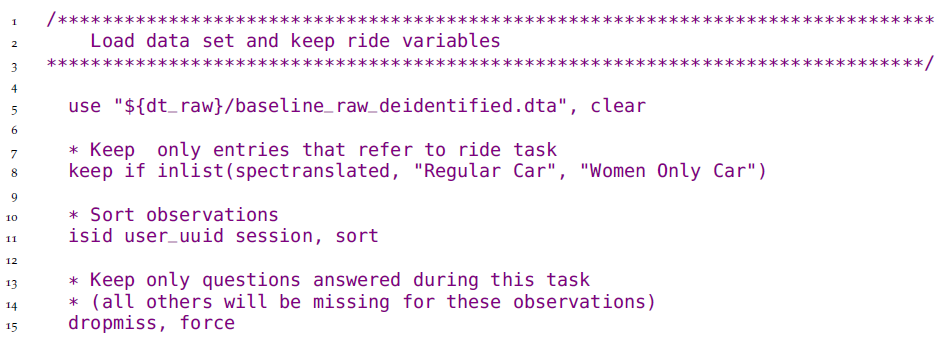
\includegraphics{examples/ch5-tidying-raw-data.png}

The script proceeds to encode categorical variables and then saves a tidy ride task dataset:

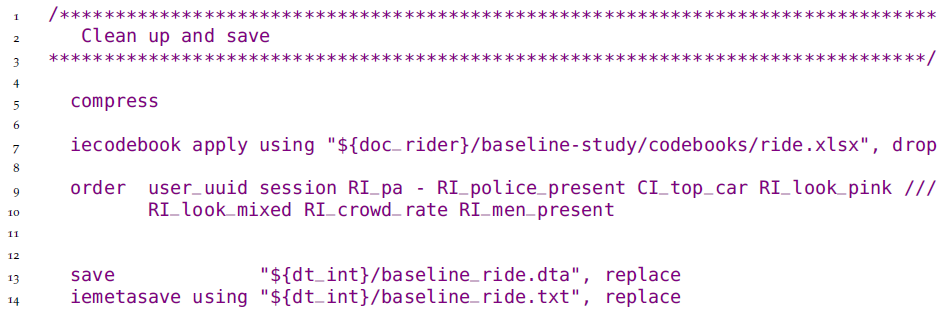
\includegraphics{examples/ch5-tidying-raw-data2.png}

The same procedure is repeated for the check-in and check-out tasks. Note that each of these tidy datasets is saved with a very descriptive name, indicating the wave of data collection and the task included in the dataset.

\begin{quote}
The complete script can be found at \url{https://git.io/Jtgqj}.
\end{quote}
\end{ex}

\hypertarget{assuring-data-quality}{%
\section*{Assuring data quality}\label{assuring-data-quality}}
\addcontentsline{toc}{section}{Assuring data quality}

Whether you are acquiring data from a partner or collecting it directly,
it is important to make sure that data faithfully reflects ground realities.
You should carefully examine and clean any data you are about to use.
When reviewing raw data, you will inevitably encounter data entry mistakes,
such as typos and inconsistent values.
Whether your team is conducting a survey or
you are receiving administrative data from a partner,
the key aspects to have in mind are
data completeness, consistency and distribution.
Data quality assurance checks should be performed as soon as the data is acquired.
When data is being collected and transferred to the team in real-time,
this means conducting high-frequency checks.
Primary data require extra attention to quality checks,
as data entry by humans is more susceptible to errors,
and the research team will be the only line of defense between
data issues and the data analysis.
Survey-specific quality monitoring protocols are discussed in Chaper 4.

\begin{ex}
\hypertarget{demand-for-safe-spaces-case-study-assuring-data-quality}{%
\subsection{Demand for Safe Spaces Case Study: Assuring Data Quality}\label{demand-for-safe-spaces-case-study-assuring-data-quality}}

The \emph{Demand for Safe Spaces} team adopted three categories of data quality assurance checks for the crowdsourced ride data. The first -- \emph{completeness} -- made sure that each data point made technical sense in that it contained the right elements, and the data as a whole covered all the expected spaces. The second -- \emph{consistency} -- made sure that real-world details were right: stations were on the right line, payments matched the value of a task, and so on. The third -- \emph{distribution} -- produced visual descriptions of the key variables of interest to make sure that any unexpected patterns observed were further investigated. Examples of the specific checks implemented are listed below:

\textbf{Completeness}

\begin{itemize}
\tightlist
\item
  Each ride must include three tasks: check-in, ride, and check-out.
\item
  Plot the number of observations per day of the week and per half-hour time-bin to make sure there are no gaps in data delivery.
\item
  Plot all observations received from each line and station combination to visualize data coverage.
\end{itemize}

\textbf{Consistency}

\begin{itemize}
\tightlist
\item
  Ensure correspondence between stations and lines. This led to the identification of mismatches that were caused by submission of lines outside the research sample. These observations were excluded from the corrected data.
\item
  Check correspondence between task and premium for riding in the women-only car. This led to the identification of a bug in the app that caused some riders to be offered the wrong premium for some tasks. These observations were excluded from the corrected data.
\item
  Check task times to make sure they were applied in the right order. The task to be completed before boarding the train comes first, then the one corresponding to the trip, and finally the one corresponding to leaving the station.
\end{itemize}

\textbf{Distribution}

\begin{itemize}
\tightlist
\item
  Compare platform observations data and rider reports of crowding and male presence to ensure general data agreement.
\item
  Visualize distribution of rides per task per day and week to ensure consistency.
\item
  Visualize patterns of presence of men in the women-only car throughout the network.
\end{itemize}
\end{ex}

\hypertarget{implementing-data-quality-checks}{%
\subsection*{Implementing data quality checks}\label{implementing-data-quality-checks}}
\addcontentsline{toc}{subsection}{Implementing data quality checks}

Data quality checks should carefully inspect key treatment and outcome variables
to ensure that the data quality of core study variables is uniformly high,
and that additional effort is centered where it is most important.
They should be run every time data is received
to flag irregularities in the acquisition progress, in sample completeness, or in response quality.
The faster issues are identified, the more likely they are to be solved.
Once the field team has left a survey area,
or high-frequency data has been deleted from a server,
it may be impossible to verify whether data points are correct or not.
Even if the research team is not receiving data in real-time,
the data owners may not be as knowledgeable about the data,
or even as responsive to the research team queries, as time goes by.
\texttt{ipacheck}\footnote{\url{https://github.com/PovertyAction/high-frequency-checks}}
is a very useful Stata command that automates some of these tasks,
regardless of the data source.

It is important to check continuously that the observations received match the intended sample.
In surveys, electronic survey software often provides case management features
through which sampled units are directly assigned to individual enumerators.
For data received from partners, such as administrative data,
this may be harder to validate.
In these cases, cross-referencing with other data sources can help to ensure completeness.
It is often the case that raw data includes duplicate or missing entries,
which may occur due to typos, failed submissions to data servers,
or other mistakes.\footnote{More details on how to deal with duplicates during surveys
  and how to track completion
  can be found on the DIME Wiki:
  \url{https://dimewiki.worldbank.org/Duplicates_and_Survey_Logs}}
Issues with data transmission often result in missing observations,
particularly when large datasets are being transferred,
or when data is being collected in locations with limited internet connection.
Keeping a record of what data was submitted,
and comparing it to the data received as soon as transmission is complete
reduces the risk of noticing that data is missing when it is no longer possible to recover it.

Once data completeness is confirmed,
observed units must be validated against the expected sample:
this is as straightforward as merging the sample list
with the data received and checking for mismatches.
Reporting errors and duplicate observations in real time allows for efficient corrections.\footnote{Read more about how to install and use \texttt{ieduplicates} and
  how the command can help you efficiently deal with duplicates
  on the DIME Wiki:
  \url{https://dimewiki.worldbank.org/ieduplicates}.}
\texttt{ieduplicates} provides a workflow for resolving duplicate entries with the data provider.
For surveys, it is also important to track data collection progress to monitor attrition,
so that it is clear early on if a change in protocols or additional tracking will be needed.\footnote{See Özler et al. (\protect\hyperlink{ref-ozler2016combining}{2016}) for an example.}
Remember to also check survey completion rates
and sample compliance by surveyors and survey teams,
and compare data missingness across administrative regions,
to identify any clusters that may be providing data of suspect quality.

Quality checks should also include checks of response quality and consistency.
For example, whether the values for each variable fall within the expected range,
and related variables do not contradict each other.\footnote{More details about real-time data quality assurance
  and links to additional resources
  can be found on the DIME Wiki:
  \url{https://dimewiki.worldbank.org/Monitoring_Data_Quality}.}
Electronic data collection systems often incorporate many quality control features,
such as range restrictions and logical flows.
Data received from systems that do not include such controls should be checked more carefully.
Consistency checks are project specific, so it is difficult to provide general guidance.
A detailed knowledge of the variables in the dataset and a careful examination of the analysis plan
is the best way to prepare.
Examples of inconsistencies in survey data would include cases where
a household reports having cultivated a plot in one module,
but does not list any cultivated crops in another.
Response consistency should be checked across all datasets, as this is much harder to automate.
For example, if two sets of administrative records are received,
one with hospital level information and one with data on each medical staff,
the number of entries in the second set of entries should match
the number of employed personnel in the first one.

Finally, no amount of pre-programmed checks can replace actually looking at the data.
Of course that doesn't mean eye checking each data point,
but rather plotting and tabulating distributions for your main variables of interest.
This will help you identify outliers and
other potentially problematic patterns that you had not foreseen.
A common source of outliers values in survey data are typos,
but they can also occur in admin data if, for example,
the unit reported changed over time,
but the data was stored with the same variable name.
Identifying unforeseen patterns in the distribution will also help you gather relevant information,
for example whether there was no harvest data because of a particular pest in the community
or if the unusual call records in a particular area caused by temporary downtime of a tower.
Analysis of metadata and paradata can also useful in assessing data quality.
For example, electronic survey software generates
automatically collected timestamps and trace histories,
showing when data was submitted, how long enumerators spent on each question,
and how many times answers were changed before or after the data was submitted.

\hypertarget{processing-confidential-data}{%
\section*{Processing confidential data}\label{processing-confidential-data}}
\addcontentsline{toc}{section}{Processing confidential data}

When implementing the steps discussed up to this point,
you are likely to be handling confidential data.
Effective data quality monitoring
frequently requires you to identify the individual observations in your dataset,
and the people or other entities who provided the information.
Using identified data allows you to quickly follow up on and resolve identified issues.
Handling confidential data such as
\textbf{personally-identifying information}\index{personally-identifying information}
requires a secure environment and, typically, decryption.
De-identifying the data will allow you to simplify that workflow,
and will also reduces the risk of harmful leaks.
This section describes how to de-identify data in order to share it with a wider audience.

\hypertarget{protecting-research-subject-privacy}{%
\subsection*{Protecting research subject privacy}\label{protecting-research-subject-privacy}}
\addcontentsline{toc}{subsection}{Protecting research subject privacy}

Most development data involves human subjects.\footnote{Read more about what extra consideration
  you must take into account when
  working with human subjects on the DIME Wiki:
  \url{https://dimewiki.worldbank.org/Protecting_Human_Research_Subjects}.}
\index{human subjects}
As a researcher, you may have access to personal information about your subjects:
where they live, how much income they have,
whether they have committed or been victims of crimes,
their names, their national identity numbers, and other sensitive data.\footnote{See Banerjee, Ferrara, and Orozco (\protect\hyperlink{ref-banerjee2019entertainment}{2019}) for an example.}
There are strict requirements for safely storing and handling personally-identifying data,
and it is the responsibility of the research team to satisfy these requirements.\footnote{More details on research ethics as well as links to tools and
  other resources related can be found on the DIME Wiki:
  \url{https://dimewiki.worldbank.org/Research_Ethics}.
  It can also be found under Pillar 1 in the DIME Research Standards:
  \url{https://github.com/worldbank/dime-standards}.}
Everyone working with human subjects research should
have completed an ethics certification course.\footnote{Protecting Human Research Participants (\url{https://phrptraining.com})
  and the CITI Program (\url{https://citiprogram.org})
  are common options.}
A plan for secure data handling is typically also required for IRB approval.

The best way to avoid risk is to minimize interactions with PII as much as possible.
First, only collect personally-identifying information that is strictly necessary for the research.
Second, avoid the proliferation of copies of identified data.
There should never be more than one copy of the raw identified dataset in the working project folder,
and it must always be encrypted.
Third, de-identify the data as early as possible in the workflow.
Even within the research team,
access to the identified data should be limited to team members who require it for their specific tasks.
Data analysis that requires identifying information is rare
and in most cases can be avoided by properly linking masked identifiers to research information
such as treatment statuses and weights, then removing unmasked identifiers.

\% De-identification vs anonymization
Once data is acquired and the data quality checks described above are completed,
the next task is typically to \textbf{de-identify} the data,
by removing or masking all personally-identifying variables.\footnote{More details and best practices related to de-identification
  as well as tools that can help you assess disclosure risks
  can be found on the DIME Wiki:
  \url{https://dimewiki.worldbank.org/De-identification}.}
\index{de-identification}
Note that it is in practice impossible to \textbf{anonymize} data.
There is always some statistical chance that an individual's identity
will be re-linked to the stored data
-- even if that data has had all directly identifying information removed --
by using some other data that becomes identifying when integrated.
For this reason, we typically recommend de-identification in two stages.
The \textbf{initial de-identification} process,
performed as soon as data is acquired, strips the data of direct identifiers,
to create a working de-identified dataset that
can be shared \emph{within the research team} without the need for encryption.
The \textbf{final de-identification} process,
performed before data is publicly released, involves
careful consideration of the trade-offs between
risk of identifying individuals and the utility of the data,
and typically requires the removal of a further level of indirect identifiers.
The rest of this section describes how to implement
both the initial and the final de-identification processes.

\hypertarget{implementing-de-identification}{%
\subsection*{Implementing de-identification}\label{implementing-de-identification}}
\addcontentsline{toc}{subsection}{Implementing de-identification}

Initial de-identification reduces risk and simplifies workflows.
Once you create a de-identified version of the dataset,
you no longer need to interact directly with the encrypted data.
Note that if the data tidying resulted in multiple raw data tables,
each will need to be de-identified separately, but
the workflow will be the same for all of them.

During the initial round of de-identification,
datasets must be stripped of personally identifying information.
To do so, you will need to identify all variables that contain such information.
For data collection, where the research team designs the survey instrument,
flagging all potentially identifying variables at questionnaire design stage
simplifies the initial de-identification process.
If you did not do that, or you received original data by another means,
there are a few tools to help flag variables with personally-identifying data.
JPAL's \texttt{PII-scan} and
IPA's \texttt{PII\_detection},
scan variable names and labels for common string patterns
associated with identifying information.\footnote{\url{https://github.com/J-PAL/PII-Scan} and
  \url{https://github.com/PovertyAction/PII_detection}.}
The World Bank's \texttt{sdcMicro}
lists variables that uniquely identify observations,
but its more refined method and
higher processing capacity requirement makes it
better suited for final de-identification.\footnote{Benschop, Machingauta, and Welch (\protect\hyperlink{ref-benschop2019statistical}{2019})}
The \texttt{iefieldkit} command \texttt{iecodebook}
lists all variables in a dataset and exports an Excel sheet
where you can easily select which variables to keep or drop.\footnote{Read more about how to install and use \texttt{iecodebook} and
  how the command can help in de-identification and other cleaning tasks
  on the DIME Wiki:
  \url{https://dimewiki.worldbank.org/iecodebook}}

Once you have a list of variables that contain confidential information,
assess them against the analysis plan and first ask yourself for each variable:
\emph{will this variable be needed for the analysis?}
If not, the variable should be dropped.
Don't be afraid to drop too many variables the first time,
as you can always go back and extract additional variables from the raw data,
but you cannot go back in time and drop a PII variable that was leaked.

For each confidential variable that is needed in the analysis, ask yourself:
\emph{can I encode or otherwise construct a variable that masks the confidential component, and
then drop this variable?}
For example, it is easy to encode identifiers for small localities like villages
and only provide a meaningless numerical indicator
showing which observations are in the same village
without revealing which villages are included in the data.
This is typically the case for most identifying information.
If the answer to either of the two questions above is yes,
all you need to do is write a script to drop the variables that are not required for analysis,
encode or otherwise mask those that are required,
and save a working version of the data.
For example:
after constructing measures of distance or area,
drop the specific geolocations in the data;
after constructing and verifying numeric identifiers in
a social network module, drop all names.
If confidential information is strictly required for the analysis and cannot be
masked or encoded,
then at least the confidential part of the data is required
to remain encrypted
and only be decrypted when used during in the data analysis process.
Using confidential data in the analysis process
does \emph{not} justify storing or sharing it in an insecure way.

After initial de-identification is complete,
your dataset will consist of one or multiple tidy,
de-identified data tables.
This is the dataset that you will interact with
during the remaining tasks described in this chapter.
Initial de-identification should not affect the usability of the data.
Note that access to the initially de-identified data
should still be restricted to the research team only,
as indirect identifiers may still present a high risk if disclosure.
It is common, and even desirable, for teams to make data publicly available
once the tasks discussed in this chapter are concluded.
This will allow other researchers to conduct additional analysis and to reproduce your finding.
Before that can be done, however,
you should further consider whether your data can be re-identified,
in a process we call \textbf{final de-identification},
which will be discussed in more detail in Chapter \ref{publication}.

\begin{ex}
\hypertarget{demand-for-safe-spaces-case-study-implementing-de-identification}{%
\subsection{Demand for Safe Spaces Case Study: Implementing De-Identification}\label{demand-for-safe-spaces-case-study-implementing-de-identification}}

The \emph{Demand for Safe Spaces} team used the \texttt{iecodebook} command to quickly drop all identifying information from the datasets as they were imported. Additionally, before publishing the datasets, the labels indicating line and station names were removed from the dataset, leaving only the underlying category number. This was done so that it would not be possible to directly reconstruct commuting habits from the public data.

The code fragment below shows an example of the initial de-identification when the data is imported. Note that the full dataset is saved in the folder for confidential data (World Bank OneDrive), and only a short codebook listing variable names, but not their content, is saved elsewhere. \texttt{iecodebook} is then used with the \texttt{drop} option to remove confidential information from the dataset before it is saved in a shared Dropbox folder. The specific variables removed in this operation contained information on the data collection team that was not needed after quality checks were implemented (\texttt{deviceid}, \texttt{subscriberid}, \texttt{simid}, \texttt{devicephonenum}, \texttt{username}, \texttt{enumerator}, \texttt{enumeratorname}) and the phone number of survey respondents (\texttt{phone\_number}).

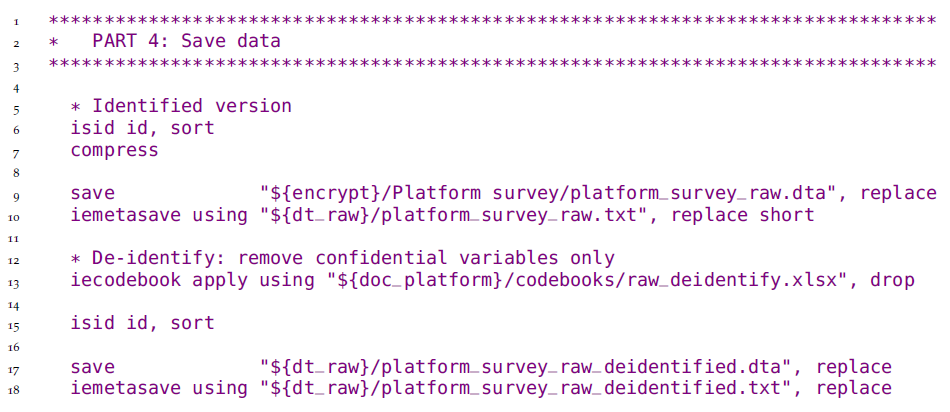
\includegraphics{examples/ch5-implementing-de-identification.png}

\begin{quote}
The complete data import do-file can be found at \url{https://git.io/JtgmU}, and the corresponding iecodebook form at \url{https://git.io/JtgmY}.
\end{quote}
\end{ex}

\hypertarget{cleaning-and-preparing-data-for-analysis}{%
\section*{Cleaning and preparing data for analysis}\label{cleaning-and-preparing-data-for-analysis}}
\addcontentsline{toc}{section}{Cleaning and preparing data for analysis}

The last step in the data cleaning process involves
making the dataset easy to use and understand, and
carefully examining each variable to document distributions
and identify patterns that may bias the analysis.
The resulting dataset will contain only the variables collected in the field, and
no modifications to data points will be made,
except for corrections of mistaken entries.
You may have more data tables in your dataset now then originally received,
and they may have a different \emph{format},
but the information contained is still the same.
Apart from the \textbf{cleaned dataset} (or datasets) itself,
cleaning will also yield extensive documentation describing it.

Data cleaning yields in-depth understanding of the contents and structure of your data.
This knowledge will be key to correctly constructing and analyzing final indicators,
which we cover in the next chapter.
Do not rush through this step!
It is common for data cleaning to be the most time-consuming task in a project.
In this section, we introduce some concepts and tools to make it more efficient and productive.
The section is separated into three subtopics:
exploring the data, making corrections, and recoding and annotating.
They are separated here because they are different in nature,
and should be kept separated in your code.
In practice, however, they may all done at the same point in time.

\hypertarget{exploring-the-data}{%
\subsection*{Exploring the data}\label{exploring-the-data}}
\addcontentsline{toc}{subsection}{Exploring the data}

The first time you interact with the data contents is during quality checks.
However, these checks are are usually time-sensitive,
and there may not be time to explore the data at length.
During data cleaning, on the other hand,
you will need to inspect each variable closely.
Use tabulations, summary statistics, histograms and density plots to understand the structure of data,
and look for patterns or irregularities.
Think critically about what you see.
You should ensure that the numerical values that appear
are consistent with the information the variable represents.
You should ensure that statistical distributions look realistic
and are not highly clumped or skewed.
You should confirm that related variables are consistent with each other.
You should check for outliers and missing values.
Then, you should assess if unusual or unexpected distributional patterns
of any of these characteristics could be caused by data entry errors.

At this point, it is more important to document your findings
than to directly address any irregularities found.
There is a very limited set of changes that should be made to the raw data during cleaning.
They are described in the next two sections,
and are usually applied to each variable as you examine it.
Most of the transformations that result in new variables
will be done during \textbf{data construction},\footnote{\textbf{Data construction:} The process of creating complex or abstract measures
  from raw information that is directly observed or collected.}\index{data construction}
a process discussed in the next chapter.
For now, focus on creating a record of what you observe,
and extensively documenting the data being explored.
You will use this documentation when discussing with your team
how to address irregularities once you get to the construction stage.
This material will also be valuable during exploratory data analysis.

\hypertarget{correcting-data-points}{%
\subsection*{Correcting data points}\label{correcting-data-points}}
\addcontentsline{toc}{subsection}{Correcting data points}

As mentioned earlier,
corrections to issues identified during data quality monitoring are
the only changes done to individual data points during the data cleaning stage.
However, there is a lot of discussion about whether one should modify such data points at all.
Some argue that follow-ups to the issues identified are costly and add limited value.
Since it is not possible to check each and every possible data entry error,
doing so can create a false sense of security from issues identified on a few main variables.
Additionally, manually-inspected data may suffer from considerable inspector variability.
In many cases, the main purpose of data quality checks
is to detect fraud and identify problems with data collection protocols.
On the other hand, there is also an argument to be made
against keeping clear typing errors or not correcting missing values.
We recommend correcting any entries that are clearly identified as errors.
However, there is some subjectivity involved in deciding
which cases fall into this category.
A common rule of thumb is to include the set of corrections
which are based on information that you have privileged access to
and other research teams would not be able to make, and no more.
Making this such decisions involve deep knowledge of the data and
the particular circumstances or each research project.

Whether you decide to modify your data or not,
you must keep a careful record of all issues that you identify.
If no data points are modified,
it may still be helpful to add flags to observations containing
potentially problematic values,
so you can verify how they affect results during analysis.
If your team decides to follow up on and correct these issues,
the follow-up process must also be thoroughly documented.
Be very careful not to include confidential information in documentation that is not securely stored,
or that you intend to release as part of a replication package or data publication.
Finally, remember not to make changes directly to the raw data.
Instead, any corrections must be done as part of data cleaning,
applied through code, and saved to a new intermediate dataset.

\begin{ex}
\hypertarget{demand-for-safe-spaces-case-study-correcting-data-points}{%
\subsection{Demand for Safe Spaces Case Study: Correcting Data Points}\label{demand-for-safe-spaces-case-study-correcting-data-points}}

Most of the issues the \emph{Demand for Safe Spaces} team identified in the raw crowdsourced data during data quality assurance were related to incorrect station and line IDs. Two steps were needed to address this issue. The first was correcting data points. The second was documenting the corrections made.

The correct values for the line and station IDs, as well as notes on how they were identified, were saved in a dataset called \texttt{station\_correction.dta}. The team used the command merge to replace the values in the raw data in memory (called the ``master data'' in \texttt{merge}) with the \texttt{station\_correction.dta} data (called the ``using data'' in \texttt{merge}).

The following options were used for the following reasons:

\begin{itemize}
\tightlist
\item
  \texttt{update\ replace} -- updates values in ``master data'' with values from the same variable in the ``using data''
\item
  \texttt{keepusing(user\_station)} -- only consider this one variable from the ``using data''
\item
  \texttt{assert(master\ match\_update)} -- confirms that all observation are either only in ``master data'' or was in both ``master data'' and ``using data'' and that the values were updated with the values in the ``using data''. This is an important quality assurance check to make sure that data was merged as expected
\end{itemize}

To document the final contents of the original data, the team published Supplemental Materials on GitHub as well as on the World Bank Microdata Catalog.

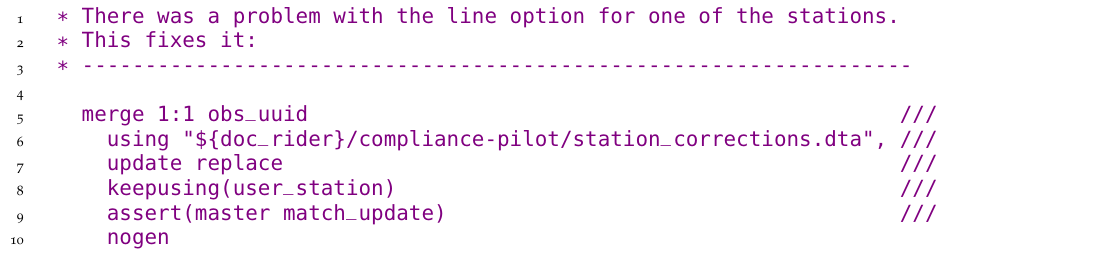
\includegraphics{examples/ch5-correcting-data-points.png}

\begin{quote}
See the full script at \url{https://git.io/Jt2ZC}
\end{quote}
\end{ex}

\hypertarget{recoding-and-annotating-data}{%
\subsection*{Recoding and annotating data}\label{recoding-and-annotating-data}}
\addcontentsline{toc}{subsection}{Recoding and annotating data}

The cleaned dataset is the starting point of data analysis.
It will be extensively manipulated to construct analysis indicators,
so it is important for it to be easily processed by statistical software.
To make the analysis process smoother,
anyone opening this dataset for the first time should have all the information needed to interact with it,
even if they were not involved in the acquisition or cleaning process.
This will save them time going back and forth between the dataset and its accompanying documentation.

Often times, datasets are not imported into statistical software in the most efficient format.
The most common example is string (text) variables:
categorical variables and open-ended responses are often read as strings.
However, variables in this format cannot be used for quantitative analysis.
Therefore, categorical variables must be transformed into other formats,
such as \emph{factors} in R and \emph{labeled integers} in Stata.\footnote{More details on value labels in Stata
  and best practices on how to work with them
  can be found on the DIME Wiki:
  \url{https://dimewiki.worldbank.org/Data_Cleaning\#Value_Labels}}
Additionally, open-ended responses stored as strings usually have a high risk of including identifying information,
so cleaning them requires extra attention.
The choice names in categorical variables
(called \emph{value labels} in Stata and \emph{levels} in R)
should be accurate, concise,
and directly linked to the data collection instrument.
Adding choice names to categorical variables
makes it easier to understand your data as you explore it,
and thus reduces the risk of small errors making their way through into the analysis stage.

In survey data, it is common for non-responses such as ``Don't know'' and ``Declined to answer''
to be represented by arbitrary survey codes.
The presence of these values could bias your analysis,
since they don't represent actual observations of an attribute.
They need to be turned into \emph{missing values}.
However, the fact that a respondent didn't know how to answer a question is also useful information
that would be lost by simply omitting all information.
In Stata, this information can be elegantly conserved using extended missing values.\footnote{More details on survey codes
  and how they relate to best practices when working with missing values in Stata
  can be found on the DIME Wiki:
  \url{https://dimewiki.worldbank.org/Data_Cleaning\#Survey_Codes_and_Missing_Values}}

We recommend that the cleaned dataset be kept as similar to the raw data as possible.
This is particularly important regarding variable names:
keeping them consistent with the raw data makes data processing and construction more transparent.
Unfortunately, not all variable names are informative.
In such cases, one important piece of documentation
makes the data easier to handle: the variable dictionary.
When a data collection instrument (for example a questionnaire) is available,
it is often the best dictionary one could ask for.
But even in these cases, going back and forth between files can be inefficient,
so annotating variables in a dataset is extremely useful.
In Stata, \texttt{variable\ labels}\footnote{More details on variable labels in Stata
  and best practices on how to work with them
  can be found on the DIME Wiki:
  \url{https://dimewiki.worldbank.org/Data_Cleaning\#Variable_Labels}}
must always be present in a cleaned dataset.
They should include a short and clear description of the variable.
A lengthier description, that may include, for example,
the exact wording of a question, may be added through \emph{variable notes}.
In R, it is less common to use variable labels,
and a separate dataset with a variable dictionary is often preferred,
but \emph{data frame attributes} can be used for the same purpose.

Finally, any information that is not relevant for analysis may be removed from the dataset.
In primary data, it is common to collect information for quality monitoring purposes,
such as notes, duration fields and surveyor IDs.
Once you are past the quality monitoring phase,
these variables may be removed from your dataset.
In fact, to make the data easier to handle,
you may choose to start from a minimal set of variables,
and add new ones as you clean them.
To ensure the cleaned dataset file doesn't get too big to be handled,
use commands such as \texttt{compress} in Stata so the data
is always stored in the most efficient format.

Although all these tasks are key to making the data easy to use,
implementing them can be quite repetitive and create convoluted scripts.
The \texttt{iecodebook} command suite, part of the \texttt{iefieldkit} Stata package,
is designed to make some of the most tedious components of this process more efficient.\footnote{Read more about how to install and use \texttt{iecodebook} and
  how the command can help making cleaning tasks more efficient
  on the DIME Wiki:
  \url{https://dimewiki.worldbank.org/iecodebook}}
\index{iecodebook}\index{iefieldkit}
It also creates a self-documenting workflow,
so your data cleaning documentation is created alongside that code,
with no extra steps.
As far as we know, currently there are no similar resources in R.
However, the \emph{tidyverse}\footnote{\url{https://www.tidyverse.org/}} packages
compose a consistent and useful grammar to perform the same tasks.

\begin{ex}
\hypertarget{demand-for-safe-spaces-case-study-recoding-and-annotating-data}{%
\subsection{Demand for Safe Spaces Case Study: Recoding and Annotating Data}\label{demand-for-safe-spaces-case-study-recoding-and-annotating-data}}

The \emph{Demand for Safe Spaces} team relied mostly on the \texttt{iecodebook} command for this part of the data cleaning process. The image below shows the \texttt{iecodebook} form used to clean the crowdsourced ride data. This process was carried out for each task.

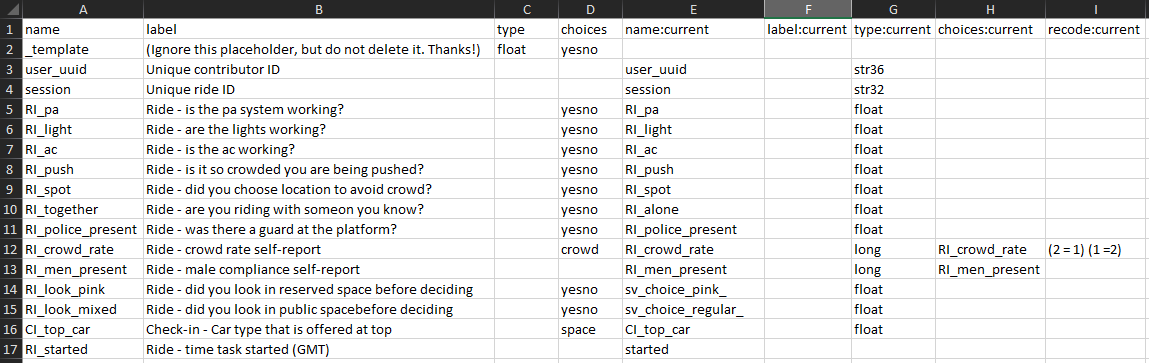
\includegraphics{examples/iecodebook.png}

Column B contains the corrected variable labels, column D indicates the value labels to be used for categorical variables, and column I recodes the underlying numbers in those variables. The differences between columns E and A indicate changes to variable names. Typically, it is strongly recommended not to rename variables at the cleaning stage, as it is important to maintain correspondence to the raw data. However, that was not possible in this case, as the same question had inconsistent variable names across multiple transfers of the data from the technology firm that managed the mobile application. In fact, this is one of the two cleaning tasks that could not be performed through \texttt{iecodebook} directly (the other was transformation of string variables to categorical format for increased efficiency). The code below shows a few examples of how these cleaning tasks were carried out directly in the script.

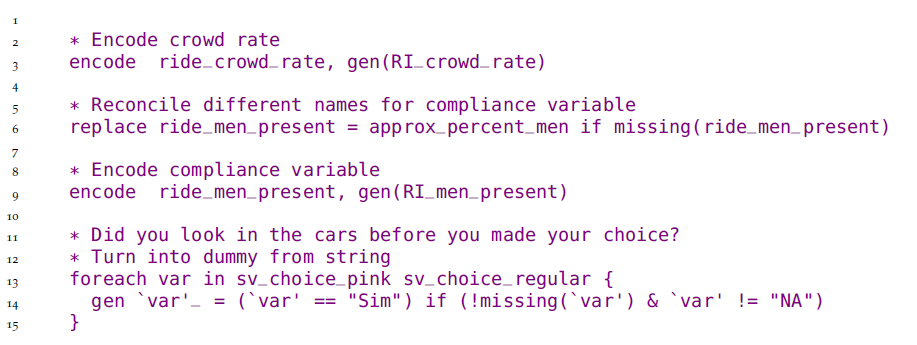
\includegraphics{examples/ch5-recording-and-annotating-data.png}

To document the contents of the original data, the team published Supplemental Materials on GitHub, including the tasks description shown in the app. All the codebooks and Excel sheets used by the code to clean and correct are also included in the \texttt{documentation} folder of the Reproducibility Package.

\begin{quote}
The complete script for cleaning the ride task can be found at \url{https://git.io/Jtgqj}, and the corresponding codebook is available at \url{https://git.io/JtgNS}.
\end{quote}
\end{ex}

\hypertarget{documenting-data-cleaning}{%
\subsection*{Documenting data cleaning}\label{documenting-data-cleaning}}
\addcontentsline{toc}{subsection}{Documenting data cleaning}

Throughout the data cleaning process,
you will often need extensive inputs from the people responsible for data collection.
Sometimes this is your research team, but often it will be someone else.
It could be a survey team, the government ministry responsible for administrative data systems,\footnote{See Fernandes, Hillberry, and Alcántara (\protect\hyperlink{ref-fernandes2015trade}{2015}) for an example.}
the technology firm that generated remote sensing data, etc.
Regardless of who originally collected the data,
you should acquire and organize all documentation of how the data was generated.\footnote{More details on how to best document your data and
  links to additional resources on this topic can be found on the DIME Wiki:
  \url{https://dimewiki.worldbank.org/Data_Documentation}}\index{documentation}
What type of documentation that is available depends on how the data was collected.
For original data collection, this should include
field protocols, data collection manuals, survey instruments,
supervisor notes, and data quality monitoring reports.
For secondary data, you should try to get the same type of information,
but that is often not possible unless
the data source is a well managed data publication.
Independently of its exact composition,
the data documentation should be stored
alongside your data dictionary and codebooks.
You will probably need these files during analysis,
and they should be published along with the data,
so other researchers may use them for their analysis as well.

\hypertarget{looking-ahead-5}{%
\section*{Looking ahead}\label{looking-ahead-5}}
\addcontentsline{toc}{section}{Looking ahead}

This chapter introduced a workflow of formatting, cleaning, and quality assurance for
the data that you obtained from the field or from partners,
illustrated in the figure that follows.
These tasks create your first research outputs using original data:
an analysis-ready dataset.
This dataset is well-structured to describe your units of analysis (it is ``tidy''),
it faithfully represents the measurements it was intended to collect,
and it does not expose the identities of the people described by it.
You have also now taken the time to fully understand the patterns and structures
in your data, and annotated and labeled them for your use and use by others.
Combined with the data map, this dataset
will be the fundamental starting point for all analysis work.
In the next chapter, we will walk through the steps needed
to run the analyses originally specified in your analysis plan
and answer your research question --
or perhaps to find out you now have even more questions.

\begin{figure}
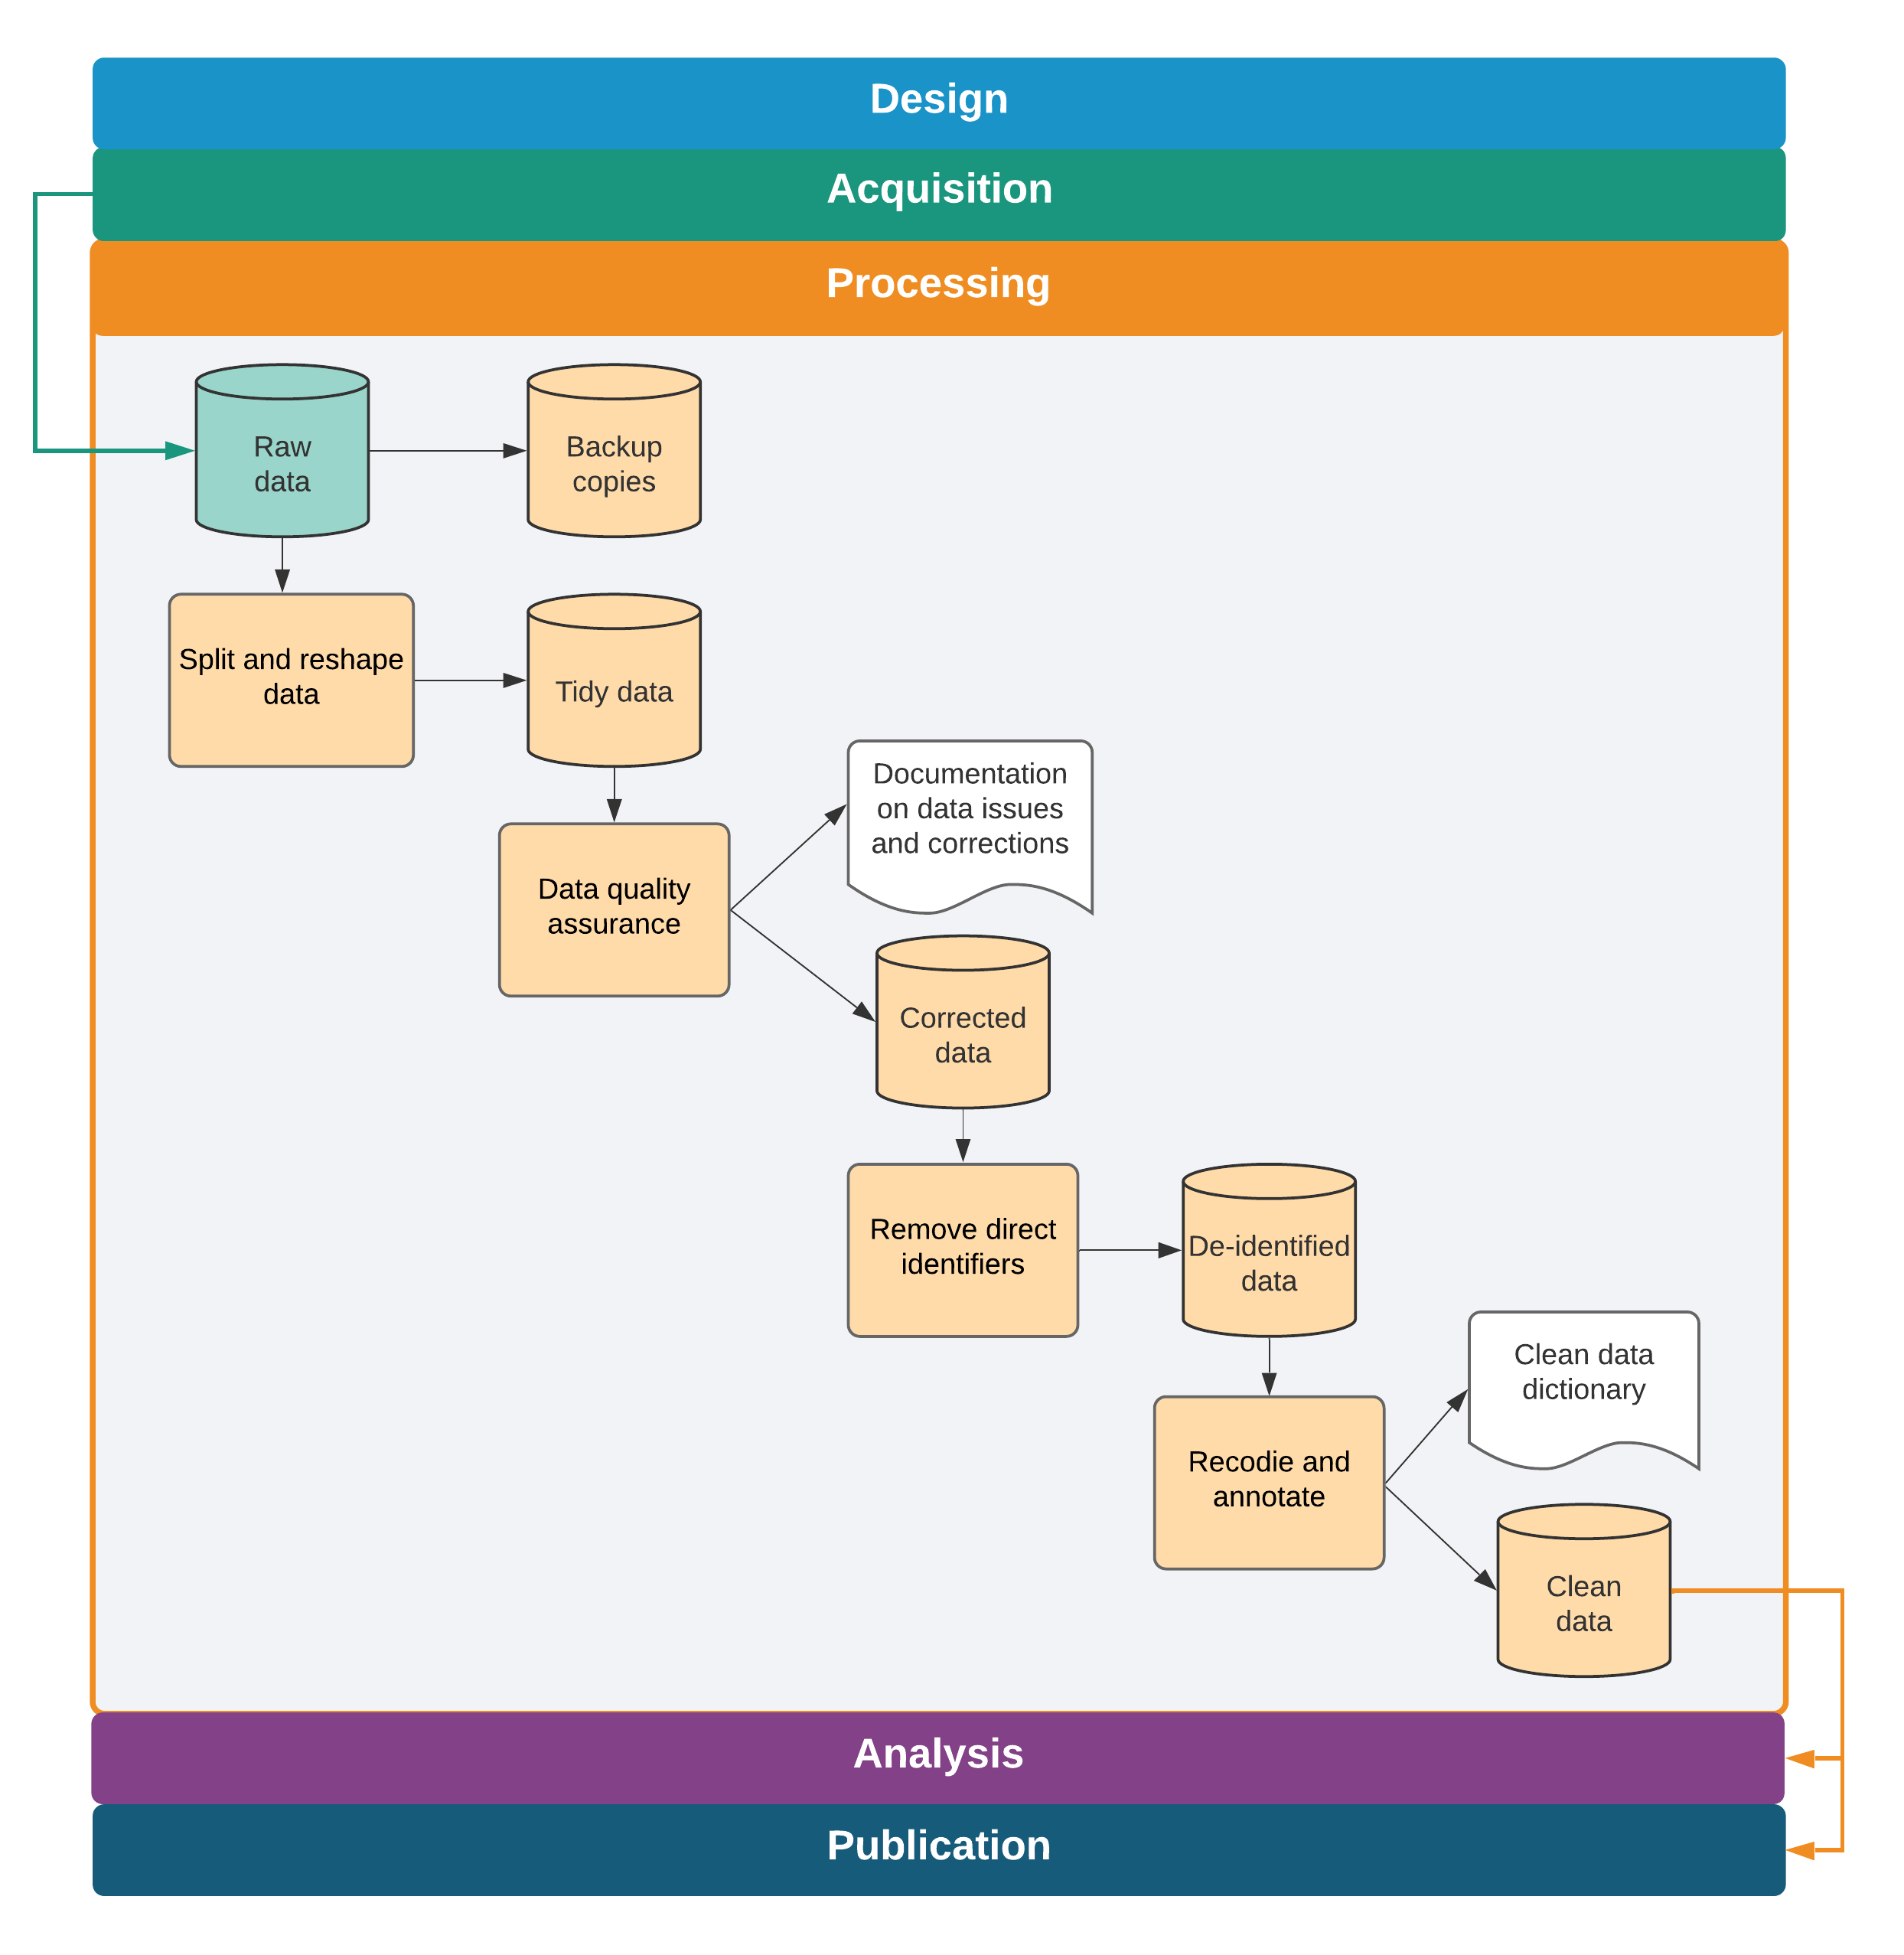
\includegraphics[width=34.9in]{diagrams/Cleaning} \caption{Data cleaning tasks and outputs}\label{fig:unnamed-chunk-34}
\end{figure}

\hypertarget{analysis}{%
\chapter{Constructing and analyzing research data}\label{analysis}}

The process of data analysis is typically
a back-and-forth discussion between people
with differing skill sets.
To effectively do this in a team environment,
data, code and outputs must be well-organized and documented,
with a clear system for version control,
analysis scripts that can be run by all team members,
and creation of research outputs fully automated.
Putting in time upfront to structure the data analysis workflow
in a reproducible manner pays substantial dividends throughout the process.
Similarly, documenting research decisions made during data analysis
is essential not only for research quality and transparency,
but also for the smooth implementation of a project.

In this chapter, we discuss the necessary steps to transform
cleaned raw data into informative analysis outputs such as tables and figures.
The suggested workflow starts where the last chapter ended:
with the outputs of data cleaning.
The first section covers variable construction:
transforming the raw data into economically meaningful indicators.
The second section discusses the analysis code itself.
We do not offer instructions on how to conduct specific analyses,
as that is determined by research design,
and there are many excellent existing guides.
Rather, we discuss how to structure and document data analysis
that is easy to follow and understand,
for both the full research team members and research consumers.
The final section discusses ways to automate common outputs
so that your work is fully reproducible.

\begin{summary}
\hypertarget{summary-constructing-and-analyzing-research-data}{%
\subsection*{Summary: Constructing and analyzing research data}\label{summary-constructing-and-analyzing-research-data}}
\addcontentsline{toc}{subsection}{Summary: Constructing and analyzing research data}

To move from raw development data to the final datasets used for analysis, you will almost certainly need to combine and transform variables into the relevant indicators and indices. These constructed variables will then be used to create analytical outputs, ideally using a dynamic document workflow. Construction and analysis involves:

\textbf{1. Constructing variables and purpose-built datasets.} Transforming pure observed data points into abstract or aggregate variables, and analyzing them properly, requires guidance from theory and is unique to each type of study. However, it should always involve the following:

\begin{itemize}
\tightlist
\item
  Maintaining \emph{separate construction and analysis scripts}, and putting the appropriate code in the corresponding script even if they are simultaneously edited and executed by the master script
\item
  \emph{Merging or otherwise combining data} from different sources or units of observation
\item
  Creating \emph{purpose-built analytical datasets}, naming and saving them appropriately, and using them for the corresponding analytical tasks, rather than building a single analytical dataset
\item
  \emph{Carefully documenting} each of these steps in plain and clear language, so that the rationale behind each research decision Is clear for any research consumer
\end{itemize}

\textbf{2. Generating and exporting exploratory and final outputs.} Tables and figures are the most common types of analytical outputs. All outputs must be well-organized and fully replicable. When creating outputs, always:

\begin{itemize}
\tightlist
\item
  Name \emph{exploratory outputs} descriptively, and store them in easily-viewed formats
\item
  Store \emph{final outputs} separately from exploratory outputs, and export using production-quality formats
\item
  \emph{Version-control all code} required to produce all outputs from analysis data
\item
  \emph{Archive code} when analyses or outputs are not likely to be used, with documentation for later recovery
\end{itemize}

\textbf{3. Set up an efficient workflow for outputs.} This means that:

\begin{itemize}
\tightlist
\item
  Exploratory analyses are \emph{immediately accessible}, ideally created with dynamic documents, and can be re-generated with a single script execution
\item
  \emph{Code and outputs are version-controlled} so it is easy to track where changes are coming from
\item
  Final figures, tables, and other code outputs are exported from the statistical software \emph{fully formatted} and the \emph{final document is updated in an automated manner}, so that no manual workflow is needed to recreate documents when changes are made
\end{itemize}

\hypertarget{takeaways-5}{%
\subsubsection*{Takeaways}\label{takeaways-5}}
\addcontentsline{toc}{subsubsection}{Takeaways}

\textbf{TTLs/PIs will:}

\begin{itemize}
\tightlist
\item
  Provide the theoretical framework for the analysis and supervise production of analytical datasets and outputs, reviewing statistical calculations and code functionality
\item
  Approve the final list of analytical datasets and their accompanying documentation
\item
  Provide rapid review and feedback for exploratory analyses
\item
  Advise on file format and design requirements for final outputs, including dynamic document structures
\end{itemize}

\textbf{RAs will: }

\begin{itemize}
\tightlist
\item
  Implement variable construction and analytical processes through code
\item
  Manage and document datasets in such a way that they are easily understood by other team members
\item
  Flag ambiguities, concerns, or gaps in translation from theoretical framework to code
\item
  Draft and organize exploratory outputs for rapid review by management
\item
  Maintain release-ready code and output organization with version control, so current versions of outputs are always accessible and final outputs are easily extracted from unused materials
\end{itemize}

\hypertarget{key-resources-5}{%
\subsubsection*{Key Resources}\label{key-resources-5}}
\addcontentsline{toc}{subsubsection}{Key Resources}

\begin{itemize}
\tightlist
\item
  DIME's \textbf{Research Assistant Onboarding Course} includes technical sessions on best practices for data construction ( \url{https://osf.io/k4tr6/}) and analysis (\url{https://osf.io/82t5e/})
\item
  \textbf{Visual libraries}: nice-looking, reproducible graphs in an easily browsable format.

  \begin{itemize}
  \tightlist
  \item
    Stata visual library: \url{https://worldbank.github.io/stata-visual-library}.
  \item
    R econ visual library: \url{https://worldbank.github.io/r-econ-visual-library}
  \end{itemize}
\item
  The blogpost \textbf{Nice and fast tables in Stata?} discusses best practices and links to code demonstrations of how to export tables from Stata \url{https://blogs.worldbank.org/impactevaluations/nice-and-fast-tables-stata}
\end{itemize}
\end{summary}

\hypertarget{creating-analysis-datasets}{%
\section*{Creating analysis datasets}\label{creating-analysis-datasets}}
\addcontentsline{toc}{section}{Creating analysis datasets}

For this chapter, we assume you are starting from
one or multiple well-documented tidy\footnote{Wickham and Grolemund (\protect\hyperlink{ref-hadley2017R}{2017})} datasets.
We also assume that these datasets
have gone through thorough quality checks
and incorporate any corrections needed.\footnote{See Chapter \ref{processing} for discussions on how to
  tidy data, monitor data quality and document corrections.}
The next step is to \textbf{construct}\footnote{\textbf{Data construction}:
  The process of transforming cleaned data into analysis data by
  creating the derived indicators that will be analyzed.}
the variables that you will use for analysis;
that is, to transform the cleaned data into analysis-ready data.
It's possible the data is ready for analysis as acquired,
but in most cases it needs to be prepared by integrating different datasets
and creating derived variables
(dummies, indices, and interactions, to name a few\footnote{See Adjognon, Soest, and Guthoff (\protect\hyperlink{ref-adjognon2019reducing}{2019}) for an example.}
).
The derived indicators you will construct should be
planned during research design\index{research design},
with the pre-analysis plan serving as a guide.\index{pre-analysis plan}
During construction, data will typically be
reshaped, merged, and aggregated to change the level of the data points
from the \textbf{unit of \emph{observation} } in the raw data
to the \textbf{unit of \emph{analysis} }.\footnote{More details on the concepts of unit of observations
  and unit of analysis
  can be found on the DIME Wiki:
  \url{https://dimewiki.worldbank.org/Unit_of_Observation}}
\index{unit of observation}\index{unit of analysis}

Each analysis dataset is built to answer an analysis question.
If the sub-samples and units of observation
vary for different pieces of the analysis,
you will probably need to create many purpose-built analysis datasets.\index{analysis datasets}
In such cases, it is not good practice
to try to create a single ``one-size-fits-all'' analysis dataset.
For a concrete example of what this means,
think of an agricultural intervention
that was randomized across villages
and only affected certain plots within each village.
The research team may want to
run household-level regressions on income,
test for plot-level productivity gains,
and check if village characteristics are balanced.
Having three separate datasets for each of these three pieces of analysis
will result in cleaner, more efficient, and less error-prone analytical code than if
you started from a single analysis dataset and repeatedly transformed it.

\hypertarget{organizing-data-analysis-workflows}{%
\subsection*{Organizing data analysis workflows}\label{organizing-data-analysis-workflows}}
\addcontentsline{toc}{subsection}{Organizing data analysis workflows}

Construction follows data cleaning and
should be treated as a separate task for two reasons.
First, this helps to clearly differentiate error corrections
(necessary for all data uses)
from creation of analysis indicators
(necessary only for specific analyses).
Second, it helps to ensure that variable definitions are
consistent across datasets.
For example, take a project that has a baseline and an endline survey.
Unless the two data collection instruments are exactly the same,
which is preferable but often not the case,
the data cleaning for each of these rounds will require different steps,
and therefore will be done separately.
However, the analysis indicators must be constructed in the exact same way,
so they are comparable.
To do this, you will require at least two separate cleaning scripts,
and a unified construction script.
Maintaining one construction script guarantees that you will not
accidentally make changes to an indicator from one round
while forgetting to update the other.

When we visualize the research workflow,
variable construction precedes data analysis,
as derivative variables need to be created before they are analyzed.
In practice, however, as you analyze the data,
it is often useful to revisit construction,
and explore different subsets and transformations of the data.
Even if construction and analysis are done concurrently,
you should always code them in separate scripts.
If every script that creates a table starts by loading a dataset,
subsetting it, and manipulating variables,
any edits to construction need to be replicated in all scripts.
This increases the chances that at least one of them
will have a different sample or variable definition.
Coding all variable construction and data transformation
in a unified script, separate from the analysis code,
prevents such problems and ensures consistency across different outputs.

\hypertarget{integrating-multiple-data-sources}{%
\subsection*{Integrating multiple data sources}\label{integrating-multiple-data-sources}}
\addcontentsline{toc}{subsection}{Integrating multiple data sources}

To create the analysis dataset,
it is typically necessary to combine information
from different data sources
or different datasets with a common source.
For the next few paragraphs,
we call such operations ``merges'',
but they are also commonly referred to as ``data joins''.
As discussed in Chapter \ref{measurement},
this process should be documented
using \textbf{data flowcharts},\footnote{More details on DIME's data flow chart template
  and an example can be found on the DIME Wiki:
  \url{https://dimewiki.worldbank.org/Data_Flow_Charts}}
and different data sources should only be combined
in accordance with the data linkage table.\footnote{More details on DIME's data linkage table template
  and an example can be found on the DIME Wiki:
  \url{https://dimewiki.worldbank.org/Data_Linkage_Table}}
For example, you may merge administrative data with survey data
in order to include demographic information in your analysis,
or you may want to integrate geographic information
in order to include location-specific controls.
To understand how to perform such operations,
you will need to consider the unit of observation for each dataset,
and their respective identifying variables.
Merges are frequent and complex operations,
which makes them a common source of error.
Whichever statistical software you are using,
take the time to read through the help file of merge commands
and make sure you understand their options and outputs.\index{merging data}

When writing the code to implement merge operations,
a few steps can help avoid mistakes.
First, before writing code to combine the datasets,
write pseudocode to understand which observations you expect to be
matched or not, and why.
When possible, determine exactly which and how many
matched and unmatched observations should result from the merge.
The best tool you have to understand this is
the three components of the data map discussed in Chapter \ref{measurement}.
Second, think carefully about whether you want to keep matched and unmatched observations,
or only specific matching outcomes (e.g.~to create a balanced panel),
and add that to the pseudocode as well.
Finally, run the code to merge the datasets,
and compare the outcome to your expectations.
Add comments to explain any exceptions,
and make it so the code will return an error in case unexpected results show up in future runs.

To avoid unintentional changes to your data,
pay close attention to merge results.
Two that require careful scrutiny are missing values and dropped observations.
Make sure to read about how each command treats missing observations:
are unmatched observations dropped, or are they kept with missing values?
Whenever possible, add automated checks in the script that throw an error message
if the result is different than what you expect,
or you may not notice changes in the outcome after running large chunks of code.
Document changes to the number of observations in your comments,
and explain why they are happening.
If your are subsetting your data by keeping only matched observations,
write down the reason why the observations differ across datasets,
as well as why you are only interested in those that matched.
The same applies when you are adding new observations from the merged dataset.

Some merges of data with different units of observation
are more conceptually complex.
Examples include: overlaying road location data with household data,
using a spatial match; combining school administrative data, such as attendance records and test scores,
with student demographic characteristics from a survey;
or linking a dataset of infrastructure access points, such as water pumps or schools,
with a dataset of household locations.
In these cases, a key part of the research contribution is figuring out
a useful way to combine the datasets.
Since the conceptual constructs that link observations from the two data sources
are important and can take many possible forms,
it is especially important for the data integration to not be treated mechanically,
and to be extensively documented, separately from other data construction tasks.

\begin{ex}
\hypertarget{demand-for-safe-spaces-case-study-integrating-multiple-data-sources}{%
\subsection{Demand for Safe Spaces Case study: Integrating Multiple Data Sources}\label{demand-for-safe-spaces-case-study-integrating-multiple-data-sources}}

The raw crowsourced data acquired for the \emph{Demand for Safe Spaces} study was received by the research team in a different level of observation than the one relevant for analysis. The unit of analysis is a ride, and each ride was represented in the raw data by three rows, one for questions answered before boarding the train, one for those answered during the trip and one for those answered after leaving the train. The \emph{Tidying raw data} example explains how the team created three different intermediate datasets for each of these tasks. To create the complete ride-level dataset, the team combined the individual task datasets. The code below shows how the team assured that all observations had merged as expected. Two different approaches depending on what you expect are shown.

The first code chunk shows the quality assurance protocol for when the team expected that all observations would exist in all datasets so that each merge would have only matched observations. To test that this was the case the team used the option \texttt{assert(3)}. When two dataset are merged in Stata each observations get the code 1, 2 or 3. 1 means that the observation only existed in the dataset in memory (called the ``master data''), 2 means that the observation existed only in the other dataset (called the ``using data'') and 3 means that they existed in both. \texttt{assert(3)} tests that all observation existed in both dataset and was coded as 3.

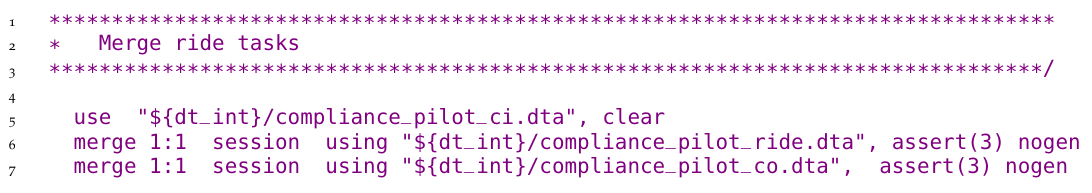
\includegraphics{examples/ch6-integrating-multiple-data-sources.png}

When merging observations that do not match perfectly, the quality assurance protocol requires that the RA document the reasons. The 1, 2, 3 merge result code explained above is saved in a variable named \texttt{\_merge}. The \emph{Demand for Safe Space} team used this variable to count the number of user IDs in each group and used the command assert to throw an error if the number of observations in any of the categories was changing, ensuring that the outcome is stable when the code is run multiple times.

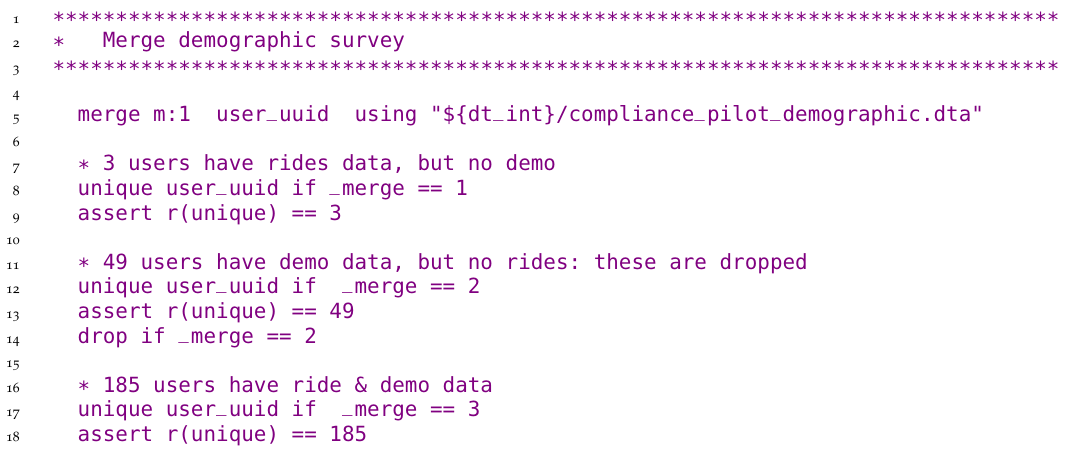
\includegraphics{examples/ch6-integrating-multiple-data-sources2.png}

\begin{quote}
See the full script at \url{https://git.io/JtgYf}
\end{quote}
\end{ex}

\hypertarget{creating-analysis-variables}{%
\subsection*{Creating analysis variables}\label{creating-analysis-variables}}
\addcontentsline{toc}{subsection}{Creating analysis variables}

Once you have assembled variables from different sources into a single working dataset
with the right raw information and observations,
it's time to create the derived indicators of interest for analysis.\index{analysis variables}
Before constructing new indicators,
you must check and double-check units, scales, and value assignments of each variable that will be used.
This is when you will use the knowledge
of the data and the documentation developed during cleaning the most.
First, check that all categorical variables have the same value assignment,
such that labels and levels have the same correspondence across variables that use the same options.
For example, it's possible that in one question \texttt{0} means ``no'' and \texttt{1} means ``yes'',
while in another one the same answers were coded as \texttt{1} and \texttt{2}.\index{binary variables}
(We recommend coding binary questions as either \texttt{1} and \texttt{0} or \texttt{TRUE} and \texttt{FALSE},
so they can be used numerically as frequencies in means and as dummies in regressions.
This often implies re-expressing categorical variables like \texttt{gender} as binary variables like \texttt{woman}.)
Second, make sure that any numeric variables you are comparing
are converted to the same scale or unit of measure:
you cannot add one hectare and two acres and get a meaningful number.
New variables should be assigned functional names,
and the dataset ordered such that related variables are together.
Adding notes to each variable will make your dataset more user-friendly.

At this point, you will also need to decide
how to handle any outliers or unusual values identified during data cleaning.
How to treat outliers is a research question.\footnote{For more details on how to deal with outliers
  see the DIME Wiki:
  \url{https://dimewiki.worldbank.org/Variable_Construction/\#Dealing_with_outliers}}\index{outliers}
There are multiple possible approaches,
and the best choice for a particular case
will depend on the objectives of the analysis.
Whatever your team decides, make sure to explicitly note
what the decision was and how it was made.
Results can be sensitive to the treatment of outliers,
so keeping the original variable in the dataset
will allow you to test how much it affects your outputs.
All these points also apply to imputation of missing values and other distributional patterns.
As a general rule, never overwrite or delete original data during the construction process.
Always create derived indicators with new names.

Two features of data create additional complexities when constructing indicators:
research designs comprising multiple units of observation and analysis,
and designs with repeated observations of the same units over time.
When your research involves different units of observation,
creating analysis datasets will probably mean combining variables measured at these different levels.
If you followed our recommendations from Chapter \ref{processing},
this means combining variables that are included in different tidy datasets.
To make sure constructed variables are consistent across datasets,
we recommend that each indicator be constructed in the dataset corresponding to its unit of observation.
Once we have indicators at each unit of observation,
they may be aggregated and/or merged to different units of analysis.
Take the example of a project that acquired data at both the student and teacher levels.
You may want to analyze the performance of students on a test
while controlling for teacher characteristics.
This can be done by assigning the teacher-level indicators to all the students in the corresponding class.
Conversely, you may want to include average student test scores
in the analysis dataset containing teacher-level variables.
To do so, you would start from the constructed dataset at student level,
average (using commands like \texttt{collapse} in Stata and \texttt{summarise} in R)
the test scores of all students taught by the same teacher,
and merge this teacher-level aggregate measure onto the original teacher dataset.
You should be mindful of two aspects while performing such operations:
the first is the correspondence between identifying variables at different levels,
which should be documented in the \textbf{data linkage table};
the second is that they will necessarily involve merges,
so all the steps outlined in the previous section should be applied.

Finally, creating a panel with survey data involves additional timing complexities.
It is common to construct indicators soon after receiving data from a new survey round.
However, creating indicators for each round separately increases the risk of using different definitions each time.
Having a well-established definition for each constructed variable helps prevent that mistake,
but the best way to guarantee it won't happen is to create the indicators for all rounds in the same script.
Say you constructed some analysis variables after baseline, and are now receiving midline data.
Then the first thing you should do is create a cleaned panel dataset,
ignoring the previous constructed version of the baseline data.
Our team created \texttt{iefieldkit}'s \texttt{iecodebook\ append} subcommand
to help you reconcile and append data from cleaned survey rounds
or similar data collected from different contexts.\footnote{Read more about how to install and use \texttt{iecodebook} and
  how the command can help appending data more efficiently
  on the DIME Wiki:
  \url{https://dimewiki.worldbank.org/iecodebook}}
\index{iefieldkit}\index{iecodebook}
This is done by completing an Excel sheet to indicate what changes in
names, value assignments, and value labels should be made so the data is consistent across rounds or settings.\footnote{See Daniels et al. (\protect\hyperlink{ref-daniels2017use}{2017}) for an example.}
By doing so, you are also creating helpful documentation about your data work.
Once data tables are consistently appended,
adapt your construction script so it can be used on the complete panel dataset.
In addition to preventing inconsistencies and documenting your work,
this process will also save you time and give you an opportunity to review your original code.

\begin{ex}
\hypertarget{demand-for-safe-spaces-case-study-creating-analysis-variables}{%
\subsection{Demand for Safe Spaces Case Study: Creating Analysis Variables}\label{demand-for-safe-spaces-case-study-creating-analysis-variables}}

The header of the script that creates analysis variables for the crowdsourced data in the \emph{Demand for Safe Spaces} study is shown below. Note that it starts from a pooled dataset that combines all waves of data collection. It is important that the variable construction is done after all waves have been pooled to make sure that all variables are constructed identically across all waves.

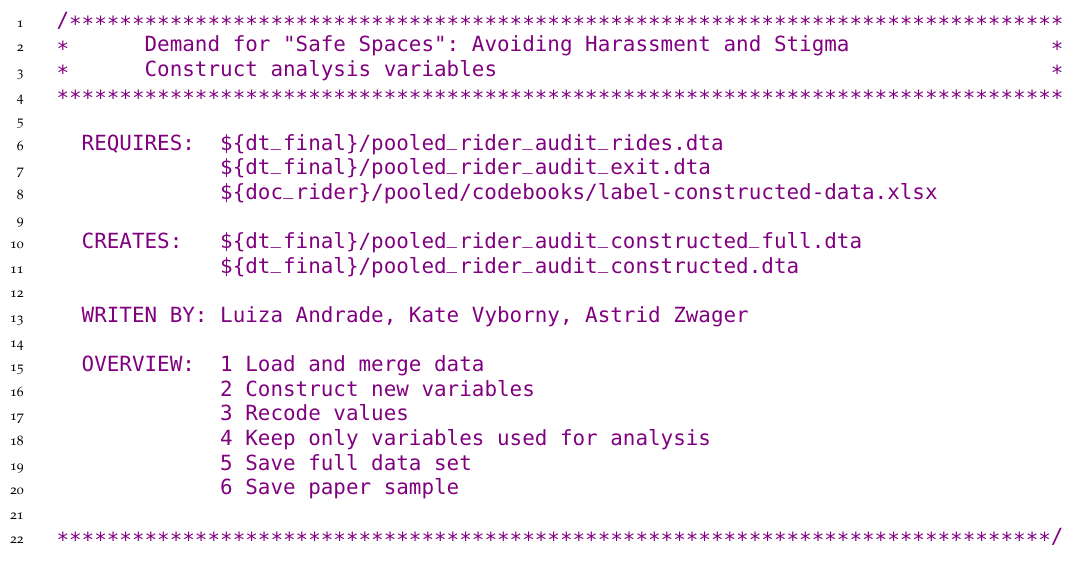
\includegraphics{examples/ch6-creating-analysis-variables.png}

\begin{quote}
See the full construction script here \url{https://git.io/JtgY5} and the script where data from all waves are pooled here: \url{https://git.io/JtgYA}.
\end{quote}
\end{ex}

\hypertarget{documenting-variable-construction}{%
\subsection*{Documenting variable construction}\label{documenting-variable-construction}}
\addcontentsline{toc}{subsection}{Documenting variable construction}

Because data construction involves translating concrete observed data points
to measures of abstract concepts,
it is important to document exactly how each variable is derived or calculated.
Careful documentation is closely linked to the research principles discussed in Chapter \ref{reproducibility}.
It makes research decisions transparent,
as anyone can read about how you defined each variable in your analysis,
and what was the reasoning behind these decisions.
By reading the documentation,
someone unfamiliar with the project should be able to understand the contents of the analysis datasets,
the steps taken to create them, and the decision-making process through your documentation.
Ideally, they should also be able reproduce your steps and recreate the constructed variables.
Therefore, documentation is an output of construction as relevant as the code and data,
and it is good practice for papers to have an accompanying data appendix
listing analysis variables and their definitions.

The development of construction documentation is a good opportunity to have
a wider discussion with your team about creating protocols for variable definition,
which will guarantee that indicators are defined consistently across projects.
You must have a detailed account of how variables are created.
This will be implemented in your code, but you should still
add comments explaining in human language what you are doing and why.
This is a crucial step both to prevent mistakes and to guarantee transparency.
To make sure that these comments can be more easily navigated,
it is wise to start writing a variable dictionary as soon as you begin making changes to the data.\footnote{See Jones et al. (\protect\hyperlink{ref-jones2019factor}{2019}) for an example.}
The variable dictionary can be saved in an Excel spreadsheet,
a Word document, or even a plain text file.
Whatever format it takes,
it should carefully record how specific variables have been combined, recoded, and scaled.
Whenever relevant, the code should point to these files to indicate
where the definition are being implemented.

The \texttt{iecodebook\ export} subcommand is
a good way to ensure you have easy-to-read documentation.
When all your final indicators have been created,
you can use it to list all variables in the dataset in an Excel sheet.
You can then add the variable definitions to that file to create a concise metadata document.
Take this opportunity to review your notes and make sure that your code
is implementing exactly what is described in the documentation.

\begin{ex}
\hypertarget{demand-for-safe-spaces-case-study-documenting-variable-construction}{%
\subsection{Demand for Safe Spaces Case Study: Documenting Variable Construction}\label{demand-for-safe-spaces-case-study-documenting-variable-construction}}

The \emph{Demand for Safe Spaces} team documented the definition of every variable used to produce the outputs presented in the paper in an Appendix to the Working Paper. Appendix B includes a set of tables with variable definitions in non-technical language. The tables include variables collected through surveys, variables constructed for analysis, and research variables assigned by random processes.

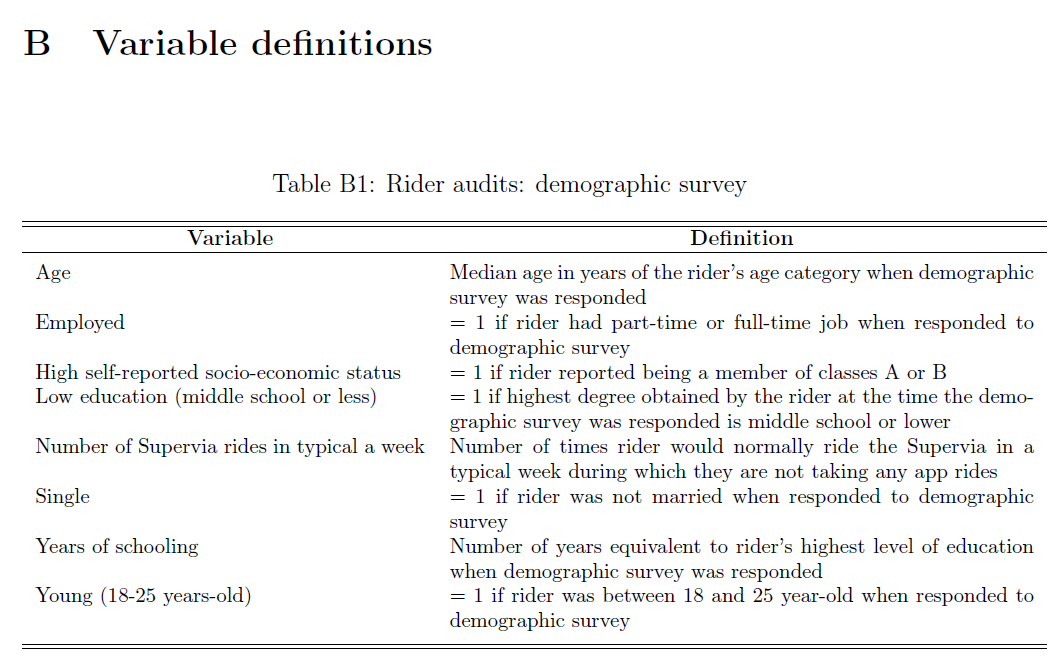
\includegraphics{examples/dictionary.png}

\begin{quote}
The full set of tables can be found on Appendix B of the Working Paper: \url{https://openknowledge.worldbank.org/handle/10986/33853}
\end{quote}
\end{ex}

\hypertarget{writing-analysis-code}{%
\section*{Writing analysis code}\label{writing-analysis-code}}
\addcontentsline{toc}{section}{Writing analysis code}

After data is cleaned and indicators are constructed, you are ready to start analyzing the data.
\index{data analysis}
There are many existing resources for data analysis and statistical methods, such as
\emph{R for Data Science};\footnote{Wickham and Grolemund (\protect\hyperlink{ref-hadley2017R}{2017})}
\emph{A Practical Introduction to Stata};\footnote{McGovern (\protect\hyperlink{ref-RePEc:gdm:wpaper:9412}{2012})}
\emph{Mostly Harmless Econometrics};\footnote{Angrist and Pischke (\protect\hyperlink{ref-angrist2008mostly}{2008})}
and \emph{Causal Inference: The Mixtape}.\footnote{Cunningham (\protect\hyperlink{ref-cunningham2018causal}{2018})}
We focus on how to structure data analysis code and files, rather than how to conduct specific analyses.

\begin{ex}
\hypertarget{demand-for-safe-spaces-case-study-writing-data-analysis-code}{%
\subsection{Demand for Safe Spaces Case Study: Writing Data Analysis Code}\label{demand-for-safe-spaces-case-study-writing-data-analysis-code}}

The \emph{Demand for Safe Spaces} team's analysis scripts are split into one script per output and the constructed data is re-loaded before each output. This ensures that final exhibit can be independently generated from the constructed data. No variable construction is done in the analysis scripts: the only data transformations performed are sub-setting the data or aggregating to a higher unit of observation. This guarantees that the same data is used across all analysis scripts. For an example of a short analysis do-file, see the code chunk below.

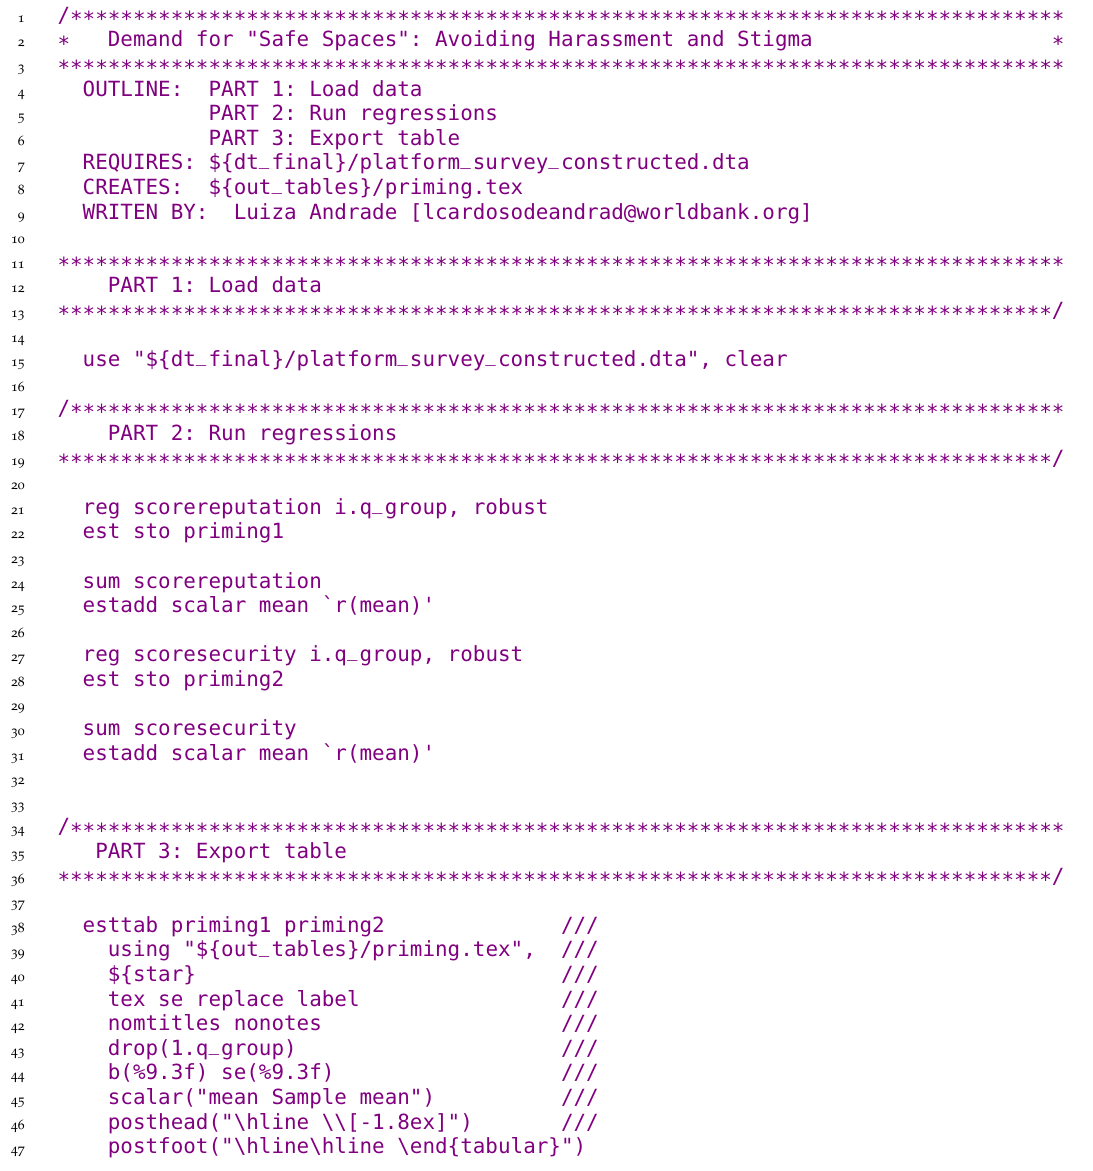
\includegraphics{examples/ch6-writing-data-analysis-code.png}

\begin{quote}
See this script and how the regression results were exported to a table at \url{https://git.io/JtgOk}.
\end{quote}
\end{ex}

\hypertarget{organizing-analysis-code}{%
\subsection*{Organizing analysis code}\label{organizing-analysis-code}}
\addcontentsline{toc}{subsection}{Organizing analysis code}

The analysis stage usually starts with a process we call \textbf{exploratory data analysis}.\index{exploratory data analysis}
This is when you are first looking for patterns in your data,
creating descriptive graphs and tables,
and trying different tests to understand your results.
It progresses into \textbf{final analysis} when your team starts to decide which are the ``main results'',
or those that will make it into a research output.
The way you deal with code and code outputs for exploratory and final analysis is different.
During the exploratory stage,
you will be tempted to write lots of analysis into one big, impressive, start-to-finish script.
While this is fine when you are writing your research stream of consciousness into code,
it leads to poor practices in the final code such as not clearing the workspace
and not loading a fresh dataset before each analysis task.

To avoid mistakes, it's important to take the time
to organize the code that you want to keep, that is,
the final analysis code, in an organized manner.
The result is a curated set of polished scripts that
will be part of a reproducibility package.\index{reproducibility package}
A well-organized analysis script starts with a completely fresh workspace
and, for each output it creates, explicitly loads data before analyzing it.
This setup encourages data manipulation to be done earlier in the workflow
(that is, in separate cleaning and construction scripts).
It also prevents the common problem of having analysis scripts
that depend on other analysis scripts being run before them.
Such dependencies tend to require manual instructions
for all necessary chunks of code to be run in the right order.
We encourage you to code each task so
it is completely independent of all other code,
except for the master script.
You can go as far as coding every output in a separate script,
but the key is making sure you know which datasets are used for each output,
and which code chunks implement each piece of analysis.

There is nothing wrong with code files being short and simple.
In fact, analysis scripts should be as simple as possible,
so whoever is reading them can focus on the concepts, not the coding.
Research questions and statistical decisions should be incorporated explicitly in the code through comments,
and their implementation should be easy to detect from the way the code is written.
This includes clustering, sampling, and controlling for different variables, to name a few.
If you have multiple analysis datasets,
each of their names should be descriptive of the sample and unit of observation they contain.
As your team comes to a decision about model specification,
you can create functions and globals (or objects) in the master script to use across scripts.
This is a good way to make sure specifications are consistent throughout the analysis.
It also makes your code more dynamic,
as it's easy to update specifications and results
through a master file without changing every script.

To create this setup,
you will need to make sure that you have an effective data management system,
including file naming, organization, and version control.
Just as for the analysis datasets,
you should name each of the individual analysis files descriptively.
Code files such as \texttt{spatial-diff-in-diff.do},
\texttt{matching-villages.R}, and \texttt{summary-statistics.py}
are clear indicators of what each file is doing, and allow you to find code quickly.
If you intend to numerically order the script files
to correspond to exhibits as they appear in a paper or report,
leave this to near publication time,
as you will constantly re-order them during data analysis.

\begin{ex}
\hypertarget{demand-for-safe-spaces-cse-study-organizing-analysis-code}{%
\subsection{Demand for Safe Spaces Cse Study: Organizing Analysis Code}\label{demand-for-safe-spaces-cse-study-organizing-analysis-code}}

The \emph{Demand for Safe Spaces} team defined the control variables in globals in the master analysis script. This guaranteed that control variables were used consistently across regressions. It also provided an easy way to update control variables consistently across all regressions when needed. In an analysis script a regression that includes all demographic controls would then be expressed as \texttt{regress\ x\ y\ \$\{demographics\}}.

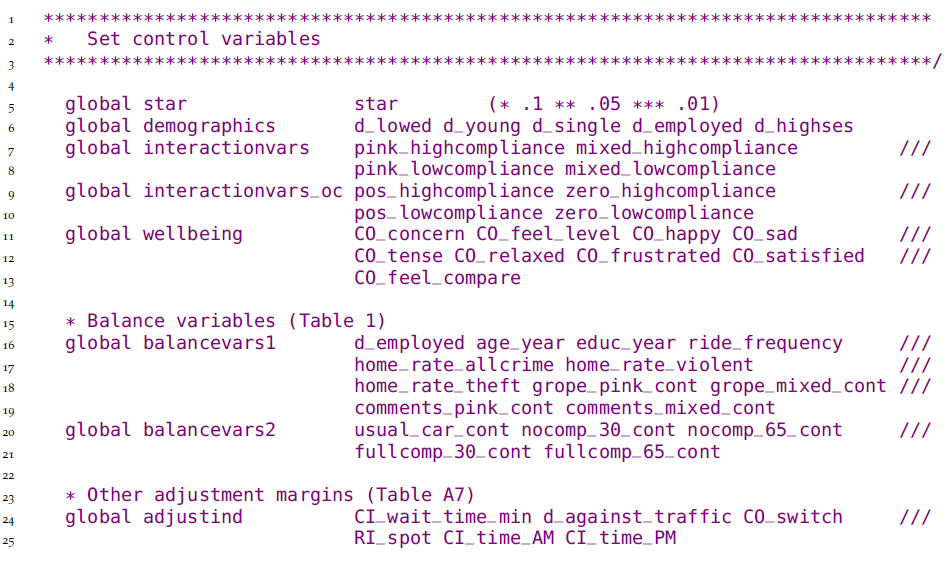
\includegraphics{examples/ch6-organizing-analysis-code.png}

\begin{quote}
The above code is excerpted from the full master script, which you can find at \url{https://git.io/JtgeT}.
\end{quote}
\end{ex}

\hypertarget{visualizing-data}{%
\subsection*{Visualizing data}\label{visualizing-data}}
\addcontentsline{toc}{subsection}{Visualizing data}

\textbf{Data visualization} is increasingly popular,
and is becoming a field in its own right.\footnote{Healy (\protect\hyperlink{ref-healy2018data}{2018}),wilke2019fundamentals}
Although the same principles for coding exploratory and final data analysis apply to visualizations,
creating them is usually more difficult than running a regression and exporting its results into a table.
We attribute some of the difficulty of creating good data visualization
to the difficulty of writing code to create them.
The amount of customization necessary to create a nice graph can lead the relevant commands to become quite intricate.
Making a visually compelling graph would already be hard enough if
you didn't have to go through many rounds of searching and reading help files
to understand a command's graphical options syntax.
Although getting each specific element of a graph to look exactly the way you want can be hard,
the solution to such problems is usually a single well-written search away,
and we recommend you leave these details as the very last adjustments to make.
In our experience, the trickiest part of using plotting commands is getting the data into the right format.
Though both Stata and R have plotting functions that graph summary statistics,
a good rule of thumb is to ensure that each
observation in your dataset corresponds to one data point in your desired visualization.
This may seem simple,
but often requires the aggregation and reshaping operations
discussed earlier in this chapter.

Based on DIME's accumulated experience creating visualizations for impact evaluations,
our team has developed a few resources to facilitate this workflow.
First of all, we maintain easily-searchable data visualization libraries for both Stata\footnote{\url{https://worldbank.github.io/Stata-IE-Visual-Library}} and R.\footnote{\url{https://worldbank.github.io/r-econ-visual-library/}}
These libraries feature curated data visualization examples, along with source code and example datasets,
so you get a good sense of what your data should look like
before you can start writing code to create a visualization.\footnote{More tools and links to other resources for creating good data visualizations
  can be found on the DIME Wiki:
  \url{https://dimewiki.worldbank.org/Data_visualization}}\index{data visualization}
The \texttt{ietoolkit} package also contains two commands to automate
common impact evaluation graphs:
\texttt{iegraph}\footnote{Read more about how to install and use \texttt{iegraph} and
  how the command can be used to easily create graphs
  for two very common impact evaluation regressions
  on the DIME Wiki:
  \url{https://dimewiki.worldbank.org/Iegraph}}
plots the values of coefficients for treatment dummies,
and \texttt{iekdensity} displays the distribution of an outcome variable
across groups and adds the treatment effect as a note.

\begin{ex}
\hypertarget{demand-for-safe-spaces-case-study-visualizing-data}{%
\subsection{Demand for Safe Spaces Case Study: Visualizing Data}\label{demand-for-safe-spaces-case-study-visualizing-data}}

The Demand for Safe Spaces team defined the settings for graphs in globals in the master analysis script. This is a simple way to create a uniform visual style for all graphs produced by the project. These globals can then be used across the project when creating graphs like this:

\texttt{twoway\ \ (bar\ cum\ x,\ color(\$\{col\_aux\_light\}))\ (lpoly\ y\ x,\ color(\$\{col\_1\}))\ (lpoly\ z\ x,\ color(\$\{col\_2\})),\ \ \ \$\{plot\_options\}}

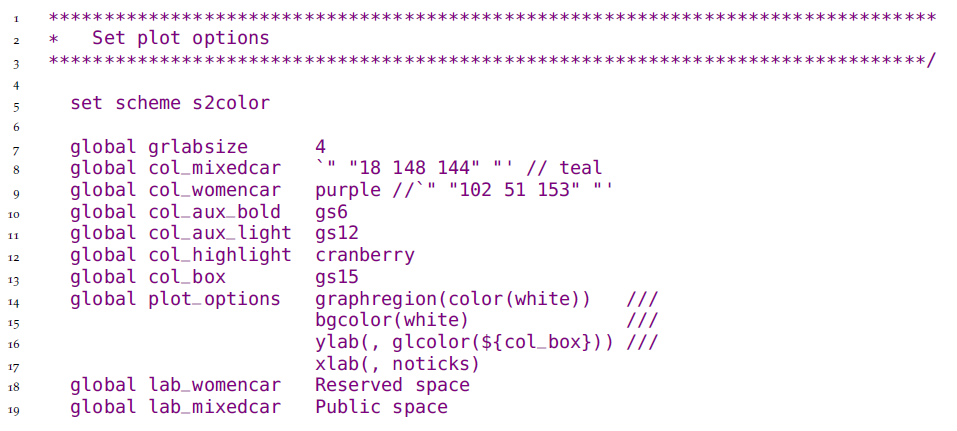
\includegraphics{examples/ch6-visualizing-data.png}

\begin{quote}
The complete script is available at \url{https://git.io/JtgeT}.
\end{quote}
\end{ex}

\hypertarget{creating-reproducible-tables-and-graphs}{%
\section*{Creating reproducible tables and graphs}\label{creating-reproducible-tables-and-graphs}}
\addcontentsline{toc}{section}{Creating reproducible tables and graphs}

A great number of outputs will be created during the course of a project.
These will include both raw outputs such as tables and graphs
and final products such as presentations, papers and reports.
During exploratory analysis, your team will consider different approaches
to answer research questions and present answers.
Though it is best to be transparent about different
specifications tried and tests performed,
only a few will ultimately be considered ``main results''.
These will be \textbf{exported}\footnote{\textbf{Exporting results:} The creation of publication-ready representations of results.}\index{exporting results}
from the statistical software.
That is, they will be saved as tables and figures in format that is easier to interact with.
For example, saving graphs as images will allow your team to quickly see them,
as well as to add them as exhibits to other documents.
When the first of these code outputs are being created, agree on where to store them,
what software and formats to use, and how to keep track of them.
This discussion will save you time and efforts on two fronts:
you will spend less time formatting and polishing tables and graphs that
will not make their way into final research products;
and you will remember the different paths your team has already
taken, so you don't do the same thing twice.
This section will take you through key elements to keep in mind
when making workflow decisions and outputting results.

\hypertarget{managing-outputs}{%
\subsection*{Managing outputs}\label{managing-outputs}}
\addcontentsline{toc}{subsection}{Managing outputs}

Decisions about storage of outputs are limited by technical constraints,
and dependent on file format.
Plain text formats like \texttt{.tex} and \texttt{.csv}
and should be managed through version control systems like Git,
as discussed in Chapter \ref{collaboration}.
Binary outputs like Excel files, PDFs, PowerPoints, or Word documents,
on the other hand, should be kept in a synced folder.
Exporting all raw outputs as plain text files,
which can be done through all statistical software,
facilitates the identification of changes in results.
When you re-run your code from the master script,
the outputs will be overwritten,
and any changes (for example, in coefficients or number of observations)
will be automatically flagged for you or a reviewer to check.
Tracking changes to binary files is more cumbersome.
They they use more space,
which may cause slow down the cloud syncing.
There may be exceptions to this general rule
depending on the Git client you are using.
GitHub Desktop, for example,
displays changes in common binary image formats such as PNG files
in an accessible manner.

You will need to update your outputs frequently.
And if you have tried to recreate a result after a few months,
you probably know that it can be hard to remember where the code that created it was saved.
File naming conventions and code organization,
including easily searchable file names and comments,
play a key role in not re-writing scripts again and again.
We recommend maintaining one ``final'' analysis folder
and one folder with draft code or exploratory analysis.
The latter contains pieces of code that are stored for reference,
but not cleaned up to be included in any final outputs.
Once an output presents a result in the clearest manner possible,
it should be renamed and moved to the ``final analysis'' folder.
It's typically desirable to have the names of outputs and scripts linked --
so, for example, \texttt{factor-analysis.do} creates \texttt{factor-analysis.eps} and so on.
Document output creation in the master script that runs your code,
so that before the line that runs a particular analysis script
there are a few lines of comments listing
datasets and functions that are necessary for it to run,
as well as all outputs created by that script.

Knowing how your code outputs will be used will help you decide the best format to export them.
You can often save figures into different formats,
such as \texttt{.eps}, \texttt{.png}, \texttt{.pdf} or \texttt{.jpg}.
However, the decision between using Office Suite software such as Word and Power Point
versus LaTeX and other plain text formats may influence how you write your code,
as this choice often implicates in the use of a particular command.
We strongly recommend that you chose software to create final products
that can be linked to raw outputs in such a way that they are updated
in the paper or presentation every time changes are made to them.
We broadly call files that have this feature \textbf{dynamic documents},\index{dynamic documents}
and they will be discussed in more detail in the final section of this chapter.

\begin{ex}
\hypertarget{demand-for-safe-spaces-case-study-managing-outputs}{%
\subsection{Demand for Safe Spaces Case Study: Managing Outputs}\label{demand-for-safe-spaces-case-study-managing-outputs}}

It is important to document which datasets are required as inputs in each script, and what datasets or files are created by each script. The \emph{Demand for Safe Spaces} team documented this both in the header of each script but also in a comment in the master do-file where the script was called.

This is a header of an analysis script called response.do that requires the file \texttt{platform\_survey\_constructed.dta} and generates the file \texttt{response.tex}. Having this information on the header allows people reading the code to check that they have access to all the necessary files before trying to run a script.

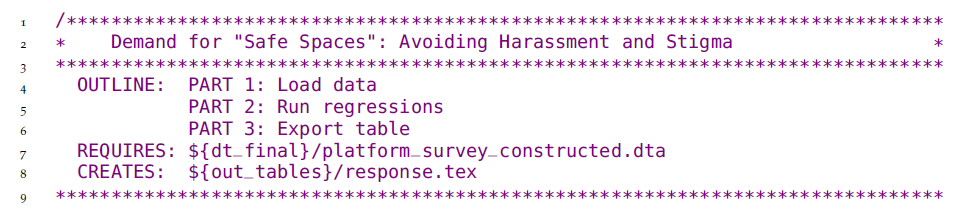
\includegraphics{examples/ch6-managing-outputs.png}

To provide the people who are interacting with the code with an overview of what are the different subscript involved in a project, this information was copied into the master do-file where the script above is called, and the same is done for all the script called from that master, as shown below.

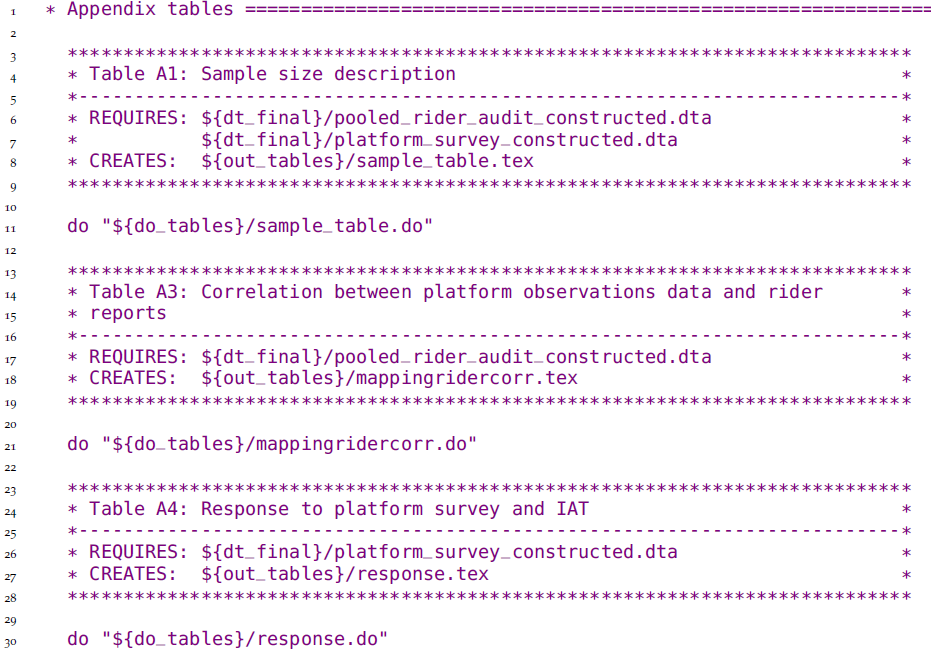
\includegraphics{examples/ch6-managing-outputs2.png}

\begin{quote}
You can find this analysis script at \url{https://git.io/JtgYB} and the master do-file at \url{https://git.io/JtgY6}.
\end{quote}
\end{ex}

\hypertarget{exporting-analysis-outputs}{%
\subsection*{Exporting analysis outputs}\label{exporting-analysis-outputs}}
\addcontentsline{toc}{subsection}{Exporting analysis outputs}

As briefly discussed in the previous section,
you do not necessarily have to export each and every table and graph
created during exploratory analysis.
Most statistical software allow you to review results interactively,
and this is often preferred at this stage.
Final analysis scripts, on the other hand, must export outputs
that are ready to be included in a paper or report.
No manual edits, including formatting,
should be necessary after exporting final outputs.
Manual edits are difficult to reproduce;
the less you need them, the more reproducible your output is.
You may think that it's not worth coding a small formatting adjustment,
but you will inevitably need to make changes to the output,
and automating them will save you time by the end of the process.
(However, don't spend much time formatting tables and graphs until
you have come to a decision about which will be used for your final product.\footnote{For a more detailed discussion on this, including different ways to export tables from Stata,
  see \url{https://blogs.worldbank.org/impactevaluations/nice-and-fast-tables-stata}}
)
Polishing final outputs can be a time-consuming process,
and you want to do it as few times as possible.

We cannot stress this enough:
do not set up a workflow that requires copying and pasting results.
Copying results from Excel to Word is error-prone and inefficient.
Copying results from a software console is risk-prone,
even more inefficient, and totally unnecessary.
The amount of work needed in a copy-paste workflow increases
rapidly with the number of tables and figures included in a research output,
and so do the chances of having the wrong version of a result in a paper or report.

There are numerous commands to export outputs from both R and Stata.
Some examples are \texttt{estout},\textsuperscript{(Jann \protect\hyperlink{ref-estout05}{2005}, @estout07)
\texttt{outreg2},}(Wada \protect\hyperlink{ref-wada2014outreg2}{2014} )
and \texttt{outwrite}\footnote{Daniels (\protect\hyperlink{ref-daniels2019outwrite}{2019})} in Stata;
and \texttt{stargazer}\footnote{Hlavac (\protect\hyperlink{ref-hlavac2015stargazer}{2015})},
\texttt{huxtable},
and \texttt{ggplot2}'s \texttt{ggsave}\footnote{Wickham (\protect\hyperlink{ref-ggplot2}{2016})}
in R.
They allow for a wide variety of output formats.
We recommend using formats that are accessible and, whenever possible, lightweight.
Accessible means that it's easy for other people to open them.
In Stata, that would mean always using \texttt{graph\ export} to save images as
\texttt{.jpg}, \texttt{.png}, \texttt{.pdf}, etc.,
instead of \texttt{graph\ save},
which creates a \texttt{.gph} file that can only be opened by Stata.
Some publications require ``lossless'' TIFF or EPS files,
which are created by specifying the desired extension.
Whichever format you decide to use,
remember to always specify the file extension explicitly.
For tables, there are fewer file format options.
Given our recommendation to use \textbf{dynamic documents},\index{dynamic documents}
which will be discussed in more detail both in the next section and in Chapter \ref{publication},
exporting tables to \texttt{.tex} is preferred.
Excel \texttt{.xlsx} and \texttt{.csv} are also commonly used,
but often require the extra step of copying the tables into the final output.
The \texttt{ietoolkit} package includes two commands to export formatted tables,
automating the creation of common outputs and saving time for research.\index{ietoolkit}
\texttt{iebaltab} creates and exports balance tables to Excel or LaTeX.\footnote{Read more about how to install and use \texttt{iebaltab}
  and how it simplifies balance tables in Stata on the DIME Wiki:
  \url{https://dimewiki.worldbank.org/iebaltab}.}\index{LaTeX}
\texttt{ieddtab} does the same for difference-in-differences regressions.\footnote{Read more about how to install and use \texttt{ieddtab}
  and how it simplifies generating tables for difference-in-differences regressions
  in Stata on the DIME Wiki:
  \url{https://dimewiki.worldbank.org/ieddtab}.}

If you need to create a table with a very specific format
that is not automated by any command you know, consider writing it manually
(Stata's \texttt{filewrite} and R's \texttt{cat()}, for example, allow you to do that).
This will allow you to write a cleaner script that focuses on the econometrics,
and not on complicated commands to create and append intermediate matrices.
Keep in mind that final outputs should be self-standing.
This means it should be easy to read and understand them with only the information they contain.
Make sure labels and notes cover all relevant information
included in your code and comments that are not otherwise visible in the output.
Examples of information that should be included in labels and notes include sample,
unit of observation, unit of measurement, and variable definition.\footnote{A checklist with best practices important to remember
  to generate informative and easy to read tables
  can be found on the DIME Wiki:
  \url{https://dimewiki.worldbank.org/Checklist:_Submit_Table}.}

\hypertarget{increasing-efficiency-of-analysis-with-dynamic-documents}{%
\section*{Increasing efficiency of analysis with dynamic documents}\label{increasing-efficiency-of-analysis-with-dynamic-documents}}
\addcontentsline{toc}{section}{Increasing efficiency of analysis with dynamic documents}

\textbf{Dynamic documents}\footnote{\textbf{Dynamic documents:} File types that include direct references
  to exported materials and update them in the output automatically.}\index{dynamic documents}
are a broad class of tools that enable a streamlined, reproducible workflow.
The term ``dynamic'' can refer to any document-creation technology
that allows the inclusion of explicitly encoded linkages to raw output files.
This means that, whenever outputs are updated,
the next time the document is loaded or compiled, it will automatically include
all changes made to all outputs without any additional intervention from the user.
This is not possible in tools like Microsoft Office,
although there are tools and add-ons that produce similar functionality.
In Word, by default, you have to copy and paste each object individually
whenever tables, graphs, or other inputs have to be updated.
This workflow becomes more complex as the number of inputs grows,
increasing the likelihood of making mistakes or missing updates.
Dynamic documents prevent this from happening by managing document compilation and
inclusion of inputs in a single integrated process,
so you can skip the copying and pasting altogether.

\hypertarget{conducting-dynamic-exploratory-analysis}{%
\subsection*{Conducting dynamic exploratory analysis}\label{conducting-dynamic-exploratory-analysis}}
\addcontentsline{toc}{subsection}{Conducting dynamic exploratory analysis}

If all team members working on a dynamic document are comfortable using the same statistical software,
built-in dynamic document engines are a good option for exploratory analysis.
With these tools,
you can write both text (often in Markdown\footnote{\url{https://www.markdownguide.org/}}) and code in the script,
and the result will usually be a PDF or HTML file including code, text, and outputs.
In our experience, many researchers find the entry cost to learning how to use these tools to be high.
These types of dynamic document tools are typically best used by the team members working most closely with code,
and can be great for creating exploratory analysis reports as you work on them,
or paper appendices including large chunks of code and dynamically created graphs and tables.
RMarkdown\footnote{\url{https://rmarkdown.rstudio.com}}
is the most widely adopted solution in R.
Stata offers a built-in package for dynamic documents, \texttt{dyndoc},\footnote{\url{https://www.stata.com/manuals/rptdyndoc.pdf}}
and user-written commands such as \texttt{markstat},\footnote{Rodriguez (\protect\hyperlink{ref-pr0067}{2017})}
\texttt{markdoc},\footnote{Haghish (\protect\hyperlink{ref-pr0064}{2016})}\\
\texttt{webdoc},\footnote{Jann (\protect\hyperlink{ref-pr0065}{2017})}
and \texttt{texdoc}.\footnote{Jann (\protect\hyperlink{ref-pr0062}{2016})}
The advantage of these tools in comparison with LaTeX is that
they create full documents from within your scripts,
so running the code and compiling the document is reduced to a single step.

Documents called ``notebooks''
(such as Jupyter Notebook\footnote{\url{https://jupyter.org}})
work similarly,
as they also use the underlying code that create the document.
These tools are usually appropriate for short or informal documents
because it tends to be difficult for those who are not familiar with them to edit the content,
and they often don't offer as extensive formatting options as, for example, Word.
There are also other simple tools for dynamic documents
that do not require direct operation of the underlying code or software,
simply access to the updated outputs.
An example of this is Dropbox Paper,
a free online writing tool that can be linked to files in Dropbox
which are automatically updated anytime the file is replaced.
These have limited functionality in terms of version control and formatting,
and may never include any references to confidential data,
but they do offer extensive collaboration features,
and can be useful for working on informal outputs.
Markdown files on GitHub can also provide similar functionality through the browser,
and are version controlled.
However, as with other Markdown options, the need to learn a new syntax may
discourage take up among team members who don't work with GitHub more extensively.

Whatever software you are using,
what matters is that you make sure to implement a self-updating process for table and figures.
We have given a few recommendations as to what we believe to be best practices,
but you will need to find out what works for your team.
If your team has decided to use Microsoft Office, for example,
there are still a few options to avoid problems with copy-pasting.
The easiest solution may be for the less code-savvy members of the team
to develop the text of the final output pointing to exhibits that are not included inline.
If all figures and tables are presented at the end of the file,
whoever is developing the code can export them into a Word document using Markdown,
so at least this part of the file can be quickly updated when the results change.
Finally, statistical programming languages can now often directly export to these formats,
such as using the \texttt{putexcel} and \texttt{putdocx} commands in Stata, which can update or respect formatting in Office documents.\footnote{See more details at
  \url{https://www.stata.com/manuals/rptputexcel.pdf}
  and \url{https://www.stata.com/stata-news/news32-3/spotlight-putdocx/}.}

\hypertarget{using-latex-for-dynamic-research-outputs}{%
\subsection*{Using LaTeX for dynamic research outputs}\label{using-latex-for-dynamic-research-outputs}}
\addcontentsline{toc}{subsection}{Using LaTeX for dynamic research outputs}

Though formatted text software such as Word and PowerPoint are still prevalent,
researchers are increasingly choosing to prepare final outputs
like documents and presentations using LaTeX.\index{LaTeX}
LaTeX is a document preparation and typesetting system with a unique code syntax.\footnote{See \url{https://github.com/worldbank/DIME-LaTeX-Templates}.}
While LaTeX has a significant learning curve,
its enormous flexibility in terms of operation, collaboration, output formatting, and styling
make it our preferred choice for most large technical outputs.
In fact, LaTeX operates behind-the-scenes in many other dynamic document tools (discussed below).
Therefore, we recommend that you learn LaTeX as soon as you are able to.

The main advantage of using LaTeX is that it updates outputs every time the document is compiled,
while still allowing for text to be added
and extensively formatted to publication-quality standards.
Additionally, because of its popularity in the academic community,
social scientists are more familiar with it than other dynamic documents tools,
so the cost of entry for a team is often relatively low.
Because \texttt{.tex} files are plain text,
they can be version-controlled using Git.
Creating documents in LaTeX using an integrated writing environment such as TeXstudio, TeXmaker or LyX
is great for outputs that focus mainly on text
and include figures and tables that may be updated.
It is good for adding small chunks of code into an output.
Finally, some journals make LaTeX templates available,
so papers can be more easily be formatted into their specific layout.

\hypertarget{looking-ahead-6}{%
\section*{Looking ahead}\label{looking-ahead-6}}
\addcontentsline{toc}{section}{Looking ahead}

This chapter discussed the steps needed to
create analysis datasets and outputs from original data.
By combining the observed variables of interest for the analysis (measurement variables)
with the information in the data map describing the study design (research variables),
you created original datasets ready for analysis,
as shown in the figure below.
Doing so is difficult, creative work,
and it is impossible to be reproduced by another person
without access to detailed records and explanations
of how you interpreted and modified the data.
You learned that code must be well-organized and well-documented
to allow others to understand how research outputs were created
and how those were used to answer the research questions.
The final chapter of this book will provide a guide
to assembling the raw findings into publishable work,
as well as describing methods for making your data,
code, documentation, and other research outputs
accessible and reusable alongside your primary outputs.

\begin{figure}
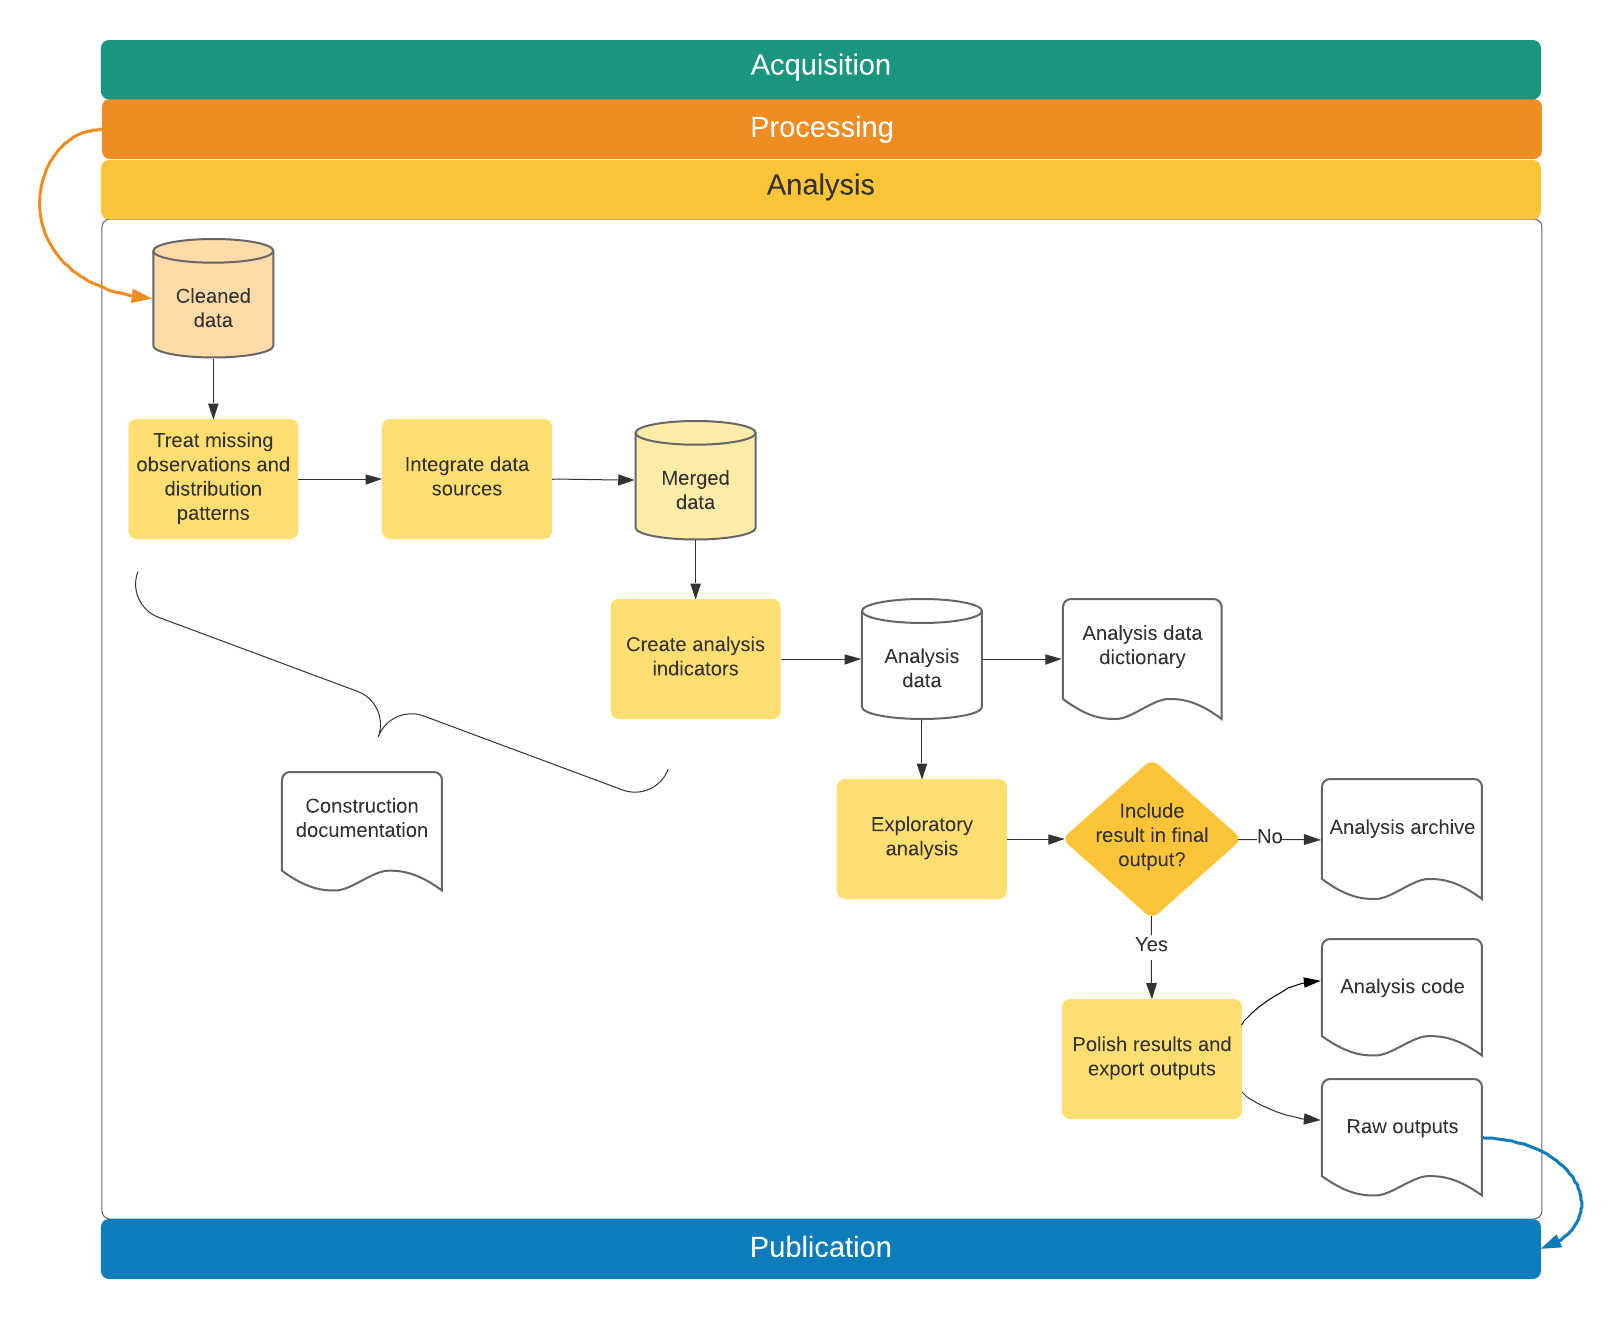
\includegraphics[width=41.51in]{diagrams/Analysis} \caption{Data analysis tasks and outputs}\label{fig:unnamed-chunk-43}
\end{figure}

\hypertarget{publication}{%
\chapter{Publishing reproducible research outputs}\label{publication}}

Publication typically involves many iterations of
data, code, and code output files, with inputs from multiple collaborators.
This process can quickly become unwieldy.
It is in nobody's interest for a skilled and busy researcher
to spend days re-numbering figures, tables, or references (and it can take days)
when a reasonable amount of up-front effort can automate the task.
Similarly, simultaneous collaboration should not involve
the repetitive and error-prone task of manually resolving
sets of tracked-changes documents with conflicting edits.
Furthermore, for most development data projects,
completing a research output is not the end of the task.
Academic journals increasingly require reproducibility packages
containing the data, code, and supporting materials
needed to recreate the results.
DIME requires reproducibility packages for all published outputs.
Replication materials represent an intellectual contribution in their own right,
because they enable others to learn from your process
and better understand the results you have obtained.
If you have organized your analysis process
according to the general principles outlined in earlier chapters,
publication will not require
substantial reorganization of the work you have already done.
Hence, publication is the conclusion of the system
of transparent, reproducible, and credible research we introduced
from the very first chapter of this book.

In this chapter, we suggest tools and workflows for
efficiently managing collaboration on research and policy outputs
and ensuring reproducible results.
The first section discusses how to use dynamic documents to collaborate on writing.
The second section covers how to prepare and publish original data,
an important research contribution in its own right.
The third section provides guidelines for preparing
functional and informative reproducibility packages.
In all cases, we note that technology is rapidly evolving
and that specific tools noted here may not remain cutting-edge,
but the core principles involved in publication and transparency will endure.

\begin{summary}
\hypertarget{summary-publishing-reproducible-research-outputs}{%
\subsection*{Summary: Publishing Reproducible Research Outputs}\label{summary-publishing-reproducible-research-outputs}}
\addcontentsline{toc}{subsection}{Summary: Publishing Reproducible Research Outputs}

Whether you are writing a policy brief or academic article, or producing some other kind of research product, you should create \textbf{three final, polished outputs} that are ready for public release (or internal archiving if not public).

\textbf{1. The data publication package.} If you collected or obtained data that you have the right to redistribute, you should make it available to the public as soon as feasible. This release should:

\begin{itemize}
\tightlist
\item
  Contain all non-identifying variables and observations \emph{originally collected} in a widely accessible format, with a \emph{data codebook} describing all variables and values
\item
  Contain \emph{original documentation} about the collection of the data, such as a survey questionnaire, API script, or data use agreement
\item
  Be \emph{modified or masked only to correct errors} or protect the privacy of people represented in the data
\item
  Be appropriately \emph{archived and licensed} with clear terms of use
\end{itemize}

\textbf{2. The research replication package.} You or your organization will typically have the rights to distribute the analytical code, even if data access is restricted. This package should:

\begin{itemize}
\tightlist
\item
  Contain all code required to \emph{derive analysis data} from the published data
\item
  Contain all code required to \emph{reproduce research outputs} from analysis data
\item
  Contain \emph{README documentation} on the use and structure of the code
\item
  Be appropriately \emph{archived and licensed} with clear terms of use
\end{itemize}

\textbf{3. The written research product(s).} These should be:

\begin{itemize}
\tightlist
\item
  Written and maintained as a \emph{dynamic document}, such as a LaTeX file
\item
  \emph{Linked} to the locations of all code outputs in the code directory
\item
  \emph{Re-compiled} with all final figures, tables, and other code outputs before release
\item
  Authored, \emph{licensed, and published} in accordance with the policies of your organization and/or publisher
\end{itemize}

\hypertarget{takeaways-6}{%
\subsubsection*{Takeaways}\label{takeaways-6}}
\addcontentsline{toc}{subsubsection}{Takeaways}

\textbf{TTLs/PIs will:}

\begin{itemize}
\tightlist
\item
  Oversee the production of outputs and know where to obtain legal or technical support if needed
\item
  Have original legal documentation available for all data
\item
  Understand the team's rights and responsibilities regarding data, code, and research publication
\item
  Decide among potential publication locations and processes for code, data, and written materials.
\item
  Verify that replication material runs and replicates the outputs in the written research product(s) exactly
\end{itemize}

\textbf{RAs will:}

\begin{itemize}
\tightlist
\item
  Rework code, data, and documentation to meet specific technical requirements of archives or publishers
\item
  Manage the production process for collaborative documents, including technical administration
\item
  Integrate comments or feedback and support proofreading, translation, typesetting, and other tasks
\end{itemize}

\hypertarget{key-resources-6}{%
\subsubsection*{Key Resources}\label{key-resources-6}}
\addcontentsline{toc}{subsubsection}{Key Resources}

\begin{itemize}
\tightlist
\item
  View published datasets in the \textbf{DIME Microdata Catalog}: \url{https://microdata.worldbank.org/index.php/catalog/dime/about}
\item
  Access our \textbf{LaTeX resources and exercises}: \url{https://github.com/worldbank/DIME-LaTeX-Templates}
\item
  Read the \textbf{DIME Research Reproducibility Standards}: \url{https://github.com/worldbank/dime-standards}
\item
  Download the Social Science Data Editors \textbf{template README}: \url{https://doi.org/10.5281/zenodo.4319999}
\end{itemize}
\end{summary}

\hypertarget{publishing-research-papers-and-reports}{%
\section*{Publishing research papers and reports}\label{publishing-research-papers-and-reports}}
\addcontentsline{toc}{section}{Publishing research papers and reports}

Development research is increasingly a collaborative effort.
This reflects changes in the economics discipline overall:
the number of sole-authored research outputs is decreasing,
and the majority of recent papers in top journals have three or more
authors.\footnote{Kuld and O'Hagan (\protect\hyperlink{ref-kuldtrend}{2017})}
As a consequence, documents typically pass back and forth between several writers
before they are ready for publication or release.
As in all other stages of the research process,
effective collaboration requires the adoption of tools and practices
that enable version control and simultaneous contributions.
This book, for example, was written in LaTeX and managed on GitHub.\footnote{\url{https://github.com/worldbank/dime-data-handbook}}
As we outlined in chapter \ref{analysis},
\textbf{dynamic documents} are a way to simplify writing workflows:
updates to code outputs that appear in these documents, such as tables and figures,
can be passed in to the final research output in a single click,
rather than copy-and-pasted or otherwise handled individually.\index{dynamic documents}
Managing the writing process in this way
improves organization and reduces error,
such that there is no risk of materials being compiled
with out-of-date results, or of completed work being lost or redundant.

\hypertarget{using-latex-for-written-documents}{%
\subsection*{Using LaTeX for written documents}\label{using-latex-for-written-documents}}
\addcontentsline{toc}{subsection}{Using LaTeX for written documents}

As we discussed in Chapter \ref{analysis}, the most widely used software
for dynamically managing formal manuscripts and policy outputs is LaTeX.
It is also becoming more popular for shorter documents,
such as policy briefs,
with the proliferation of skills and templates for these kinds of products.\index{LaTeX}
LaTeX uses explicit references to the file path of each input (such as tables and figures),
which are reloaded from these locations every time the final document is compiled.
This is not possible by default in, for example, Microsoft Word.
There, you have to copy and paste each object
whenever tables, graphs, or other inputs are updated.
As time goes on, it becomes increasingly likely
that a mistake will be made or something will be missed.
In LaTeX, instead of writing in a
``what-you-see-is-what-you-get'' mode as you do in Word,
you write plain text in a \texttt{.tex} file,
interlaced with coded instructions formatting the document and linking to exhibits (similar to HTML).
LaTeX manages tables and figures dynamically
and includes commands for simple markup
like font styles, paragraph formatting, section headers and the like.
It includes special controls for
footnotes and endnotes, mathematical notation, and bibliography preparation.
It also allows publishers to apply global styles and templates to already-written material,
reformatting entire documents in house styles with only a few keystrokes.

While LaTeX \emph{can} produce complex formatting,
this is rarely needed for academic publishing,
as academic manuscripts will usually be reformatted
based on the style of the publisher.
(By contrast, policy and other self-produced documents may desire
extensive typesetting and investments in custom templates and formatting.)
In academia at least,
it's rarely worth the investment to go beyond basic LaTeX tools:
the title page, sections and subsections,
figures and tables, mathematical equations,
bolding and italics, footnotes and endnotes,
and, last but not least, references and citations.
We acknowledge that many of these functionalities
including dynamic updating of some outputs
can be achieved in Microsoft Word
through the use of plugins and careful workflows.
If you can maintain such a workflow,
that is an acceptable approach to the same problem,
but we recommend moving towards adoption of LaTeX
when it is possible for you and your team.

One of the most important tools available in LaTeX
is the BibTeX citation and bibliography manager.\footnote{Kopka and Daly (\protect\hyperlink{ref-kopka1995guide}{1995})}
BibTeX keeps all the references you might use in a \texttt{.bib} file,
then references them using a simple command typed directly in the document.
Specifically, LaTeX inserts references in text using the \texttt{cite} command.\index{bibliography management}
Once this is written, LaTeX automatically pulls all the citations into text
and creates a complete bibliography based on the citations you used whenever you compile the document.
The system allows you to specify exactly how references should be displayed in text
(such as superscripts, inline references, etc.)
as well as how the bibliography should be styled and in what order
(such as Chicago, MLA, Harvard, or other common styles).
The same principles that apply to figures and tables are therefore applied here:
You can make changes to the references in one place (the \texttt{.bib} file),
and then everywhere they are used they are updated correctly with one process.
BibTeX is so widely used that it is natively integrated in Google Scholar.
Since different publishers have different requirements,
it is quite useful to be able to adapt this and other formatting very quickly,
including through using publisher-supplied templates where available.

Because it follows a standard code format,
LaTeX has one more useful trick:
you can convert the raw document into Word
or a number of other formats
using utilities such as \texttt{pandoc}.\footnote{\url{https://pandoc.org}}
Even though conversion to Word is required
for a number of academic publishers and can even be preferred for some policy outputs,
we still recommend using LaTeX to prepare these when possible.
You should export to Word only at the final stage, when submitting materials.
You can also use a CSL (Citation Styles Library) file\footnote{\url{https://github.com/citation-style-language/styles}}
for nearly any journal and have it applied automatically in this process.
Therefore, even in the case where you are required to provide
`.docx\} versions of materials to others, or tracked-changes versions,
you can create them effortlessly from a LaTeX document,
then use external tools like Word's compare feature
to generate integrated track-changes versions when needed.

\hypertarget{getting-started-with-latex-as-a-team}{%
\subsection*{Getting started with LaTeX as a team}\label{getting-started-with-latex-as-a-team}}
\addcontentsline{toc}{subsection}{Getting started with LaTeX as a team}

Getting used to LaTeX can be challenging,
but the control it offers over the writing process is invaluable.
Because it is written in a plain text file format,
\texttt{.tex} can be version-controlled using Git.
This makes it possible to manage contributions and version histories
using the same system we recommend for data work.
DIME Analytics has created a variety of templates and resources
that you can adapt for your own team.\footnote{\url{https://github.com/worldbank/DIME-LaTeX-Templates}}
Integrated editing and compiling tools like TeXStudio\footnote{\url{https://www.texstudio.org}}
and \emph{atom-latex}\footnote{\url{https://atom.io/packages/atom-latex}}
offer the most flexibility to work with LaTeX in teams.

Although ultimately worth it, setting up LaTeX environments locally is not always simple,
particularly if you are new to working with plain text code and file management.
This is because LaTeX requires that all formatting be done in its special code language,
and it is not always informative when you do something wrong.
This can be off-putting very quickly for people
who simply want to get to writing,
and staff not used to programming may not easily acquire the necessary knowledge.

Cloud-based implementations of LaTeX can make it easier for your team to use
LaTeX without all members having to invest in new skills
or set up matching software environments,
and can be particularly useful for first forays into LaTeX writing.
One example of this is Overleaf.\footnote{\url{https://www.overleaf.com/}}
Most such sites offer a subscription feature
with useful extensions and various sharing permissions,
and some offer free-to-use versions with basic tools that are sufficient
for a broad variety of applications,
up to and including writing a complete academic paper with coauthors.

Cloud-based implementations of LaTeX have several advantageous features
for teams compared to classic desktop installations.
First, since they are completely hosted online,
they avoid the inevitable troubleshooting required to set up a LaTeX installation
on various personal computers run by the different members of a team.
Second, they typically maintain a single, continuously synced, master copy of the document
so that different writers do not create conflicted or out-of-sync copies,
or need to deal with Git themselves to maintain that sync.
Third, they typically allow collaborators to edit documents simultaneously,
though different services vary the number of collaborators and documents allowed at each tier.
Fourth, some implementations provide a ``rich text'' editor
that behaves pretty similarly to familiar tools like Word,
so that collaborators can write text directly into the document without worrying too much
about the underlying LaTeX coding.
Cloud services also usually offer a convenient selection of templates
so it is easy to start up a project and see results right away
without needing to know a lot of the code that controls document formatting.

Cloud-based implementations of LaTeX also have disadvantages.
There is still some up-front learning required, unless you're using the rich text editor.
Continuous access to the internet is necessary,
and updating figures and tables requires a bulk file upload that is tough to automate.
Although some services offer ways to track changes and even to integrate a git workflow,
doing version control is not as straightforward as using git locally.
Finally, they also vary dramatically in their ability to integrate
with file systems where you store your code and code outputs,
and so you will need to practice an integrated workflow depending what is available to you.
Some teams adopt cloud-based tools as a permanent solution,
though our recommendation is to eventually shift to
local editing and compiling using tools such as TexStudio and code editors like Atom.

\begin{ex}
\hypertarget{demand-for-safe-spaces-case-study-publishing-research-papers-and-reports}{%
\subsection{Demand for Safe Spaces Case Study: Publishing Research Papers and Reports}\label{demand-for-safe-spaces-case-study-publishing-research-papers-and-reports}}

The \emph{Demand for Safe Spaces} project, among other outputs, produced both a policy brief and a working paper. The policy brief was produced in accordance with DIME communications protocols. For its production, the graphs exported by R and Stata were saved in EPS format and shared with a designer that adapted them to fit DIME's visual identity. The research paper was written in LaTeX through the overleaf platform, and published on the World Bank Policy Research Working Paper Series under ID 9296.


\includegraphics[width=0.62\textwidth,height=\textheight]{examples/WPS.png}
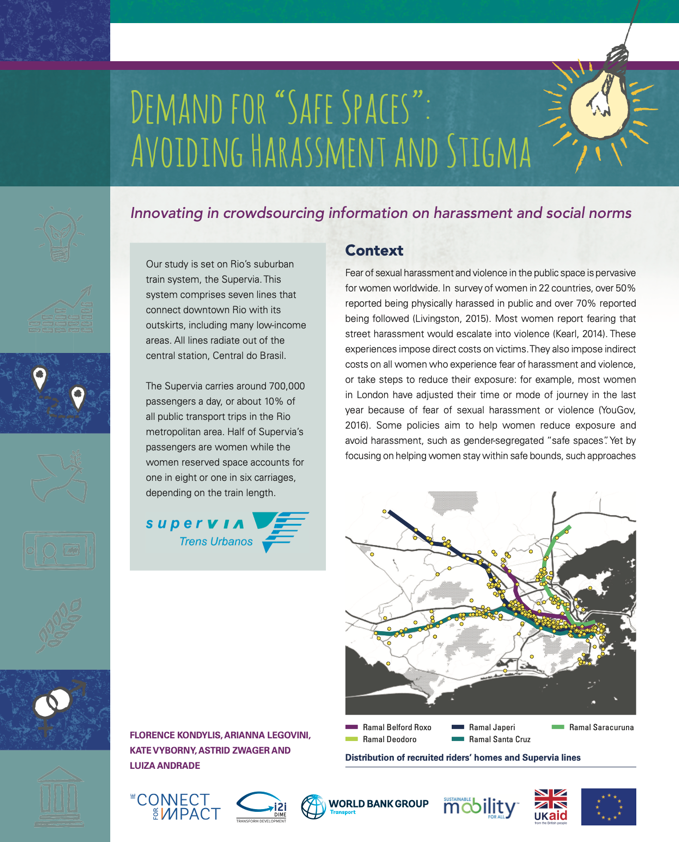
\includegraphics[width=0.37\textwidth,height=\textheight]{examples/brief.png}

\begin{quote}
The policy brief can be viewed at \url{http://pubdocs.worldbank.org/en/223691574448705973/Policy-Brief-Demand-for-Safe-Spaces.pdf}.
\end{quote}

\begin{quote}
The working paper can be viewed at \url{https://openknowledge.worldbank.org/handle/10986/33853}.
\end{quote}
\end{ex}

\hypertarget{preparing-research-data-for-publication}{%
\section*{Preparing research data for publication}\label{preparing-research-data-for-publication}}
\addcontentsline{toc}{section}{Preparing research data for publication}

While we have focused so far on written materials,
you must also consider how you will publish
the data used in your research.
The open science community at large sees data publication
both as a citable output and as a necessary transparency measure.
Fortunately, it is a conceptually simple task to produce
and catalog the required materials.
You should be prepared to catalog two separate collections.
First, you should catalog the clean data
with all variables corresponding directly
to fields in the original dataset or data collection instrument
(this will not be necessary if you are working with secondary data
that was not produced by your team,
but you will still need to carefully explain the process of acquiring this data).
If you follow the steps outlined in Chapter \ref{processing},
when you get to the publication stage you will have
a cleaned data set and supporting documentation ready.

Second, you should separately catalog
the analysis dataset used for the research output you are publishing.
This is typically included in the replication package for the research output,
and should assume that another researcher is starting work
with only the published clean data in hand.\footnote{For an example, see the replication package for Kondylis et al. (\protect\hyperlink{ref-kondylis2020demand}{2020})
  in \url{https://github.com/worldbank/rio-safe-space}.}
The package should also include the data construction scripts
that create transformed and derived indicators,
project-specific information
such as treatment assignment and other indicators
generated directly by the research team (another example is constructed record linkages).
If you followed the workflow recommended in Chapter \ref{analysis},
by the time you reach publication stage you will already have all necessary
files and documentation at hand.

\hypertarget{de-identifying-data-for-publication}{%
\subsection*{De-identifying data for publication}\label{de-identifying-data-for-publication}}
\addcontentsline{toc}{subsection}{De-identifying data for publication}

Before publishing data,
you should carefully perform a \textbf{final de-identification}.
The objective of de-identification is to reduce the risk of disclosing confidential information in the published dataset.
If you are following the workflow outlined in this book,
you should have already removed direct identifiers as a first step after acquiring the data
(see the discussion of initial de-identification in Chapter \ref{processing}).
For the final de-identification, you should additionally remove
indirect identifiers, and assess the statistical disclosure risk of your data.\footnote{\textbf{Disclosure risk:} the likelihood that a released data record can be associated with an individual or
  organization.}\index{statistical disclosure}
Unlike direct identifiers, for which a link (or lack thereof) to public information is verifiable,
indirect identifiers require an assessment of the likelihood
that an individual can be singled out in the data
and then linked to public information using combinations of available data.
For example, seemingly innocuous variables such as US zip code,
gender, and date of birth uniquely identify
approximately 87\% of the US population.\footnote{Sweeney (\protect\hyperlink{ref-Sweeney2000}{2000})}
In development data, information such as the size of a household,
the ages and marital statuses of the household members,
and the types of work or schooling they engage in
may be more than enough to identify a person or family
from a sufficiently small group.

A number of tools have been developed to help researchers de-identify data.\index{final de-identification}
At this stage, the World Bank's \texttt{sdcMicro} tool,\footnote{Benschop, Machingauta, and Welch (\protect\hyperlink{ref-benschop2019statistical}{2019})}
has a useful feature
that allows you to assess the uniqueness of the records in your data.
It produces simple measures of the identifiability of records from
the combination of potentially indirectly identifying variables,
and allows you to apply common information masking algorithms,
such as binning, top-coding, and jittering data prior to release.
You should determine how sensitive your results are to these transformations;
it may be the case that masked data cannot be used for your reproducibility package.

There will almost always be a trade-off between accuracy and privacy.
For publicly disclosed data, you should favor privacy.
Stripping identifying variables from a dataset may not be sufficient to protect respondent privacy,
due to the risk of re-identification.
One solution is to add noise to data, as the U.S. Census Bureau has proposed.\footnote{Abowd (\protect\hyperlink{ref-abowd2018us}{2018})}
This makes the trade-off between data accuracy and privacy explicit.
But there are not, as of yet, established norms for such ``differential privacy'' approaches:
most approaches fundamentally rely on judging ``how harmful'' information disclosure would be.
The fact remains that there is always a balance between information release (and therefore transparency)
and privacy protection, and that you should engage with it actively and explicitly.
The best thing you can do is make a complete record of the steps that have been taken
so that the process can be reviewed, revised, and updated as necessary.

Removing variables results in loss of information, so the de-identification process
requires careful assessment of the potential risk to the individual
that could be caused by disclosure of their identity or personal information.
This will vary widely depending on the types of information
you are collecting and the overall vulnerability of the population.
In extreme cases, where the population is highly vulnerable
and combinations of information are highly specific,
you may not be able to publicly release any data at all.
You will still be expected to catalog and cite your data,
even if you cannot release it publicly.
In practice, this may mean publishing only a catalog entry
providing information about the contents of the datasets
and how future users might request permission to access them
(even if you are not the person to grant that permission).
In some cases, it may be possible to release the dataset but
embargoing specific variables that are required for the analysis but cannot be released publicly.
It may be necessary to grant access to the embargoed data for specific purposes,
such as a computational reproducibility check required for publication,
if done under careful data security protocols and approved by an IRB.

\hypertarget{publishing-research-datasets}{%
\subsection*{Publishing research datasets}\label{publishing-research-datasets}}
\addcontentsline{toc}{subsection}{Publishing research datasets}

Publicly documenting all original data acquired as part of a research project
is an important contribution in its own right.
Cataloging and/or archiving original datasets
is a significant contribution in addition to any publication of analysis results.\footnote{More details and links to best practices on topics related to data publication,
  such as de-identification and how to license your published data,
  can be found on the DIME Wiki:
  \url{https://dimewiki.worldbank.org/Publishing_Data}.
  More details can also be found under Pillar 5 in the DIME Research Standards:
  \url{https://github.com/worldbank/dime-standards}.}\index{data licensing}
Publicly releasing data allows other researchers
to validate the mechanical construction of your results,
investigate what other results might be obtained from the same population,
and test alternative approaches or answer other questions.
This fosters collaboration and may enable researchers to explore variables and
questions that you do not have time to focus on otherwise.

The first step toward data publication is choosing the platform
where you will publish your data.\index{publishing data}
A variety of options exist;
it is important to choose one that allows you to obtain a digital object identifier (DOI)
for the location of your data (even if its URL changes),
and a formal citation for your data, so you can reference it in other research outputs.\footnote{\url{https://www.doi.org}}
Two common platforms for development data are the World Bank's Development Data Hub
and Harvard University's Dataverse.
The World Bank's Development Data Hub\footnote{\url{https://datacatalog.worldbank.org}}
includes a Microdata Catalog\footnote{\url{https://microdata.worldbank.org}}
and a Geospatial Catalog,
where researchers can publish data and documentation for their projects.\footnote{More details on how to submit to the World Bank Microdata Catalog and
  links to DIME's submissions there can be found on the DIME Wiki:
  \url{https://dimewiki.worldbank.org/Microdata_Catalog}}
The Harvard Dataverse publishes both data and code,
and its Datahub for Field Experiments in Economics and Public Policy\footnote{\url{https://dataverse.harvard.edu} and
  \url{https://dataverse.harvard.edu/dataverse/DFEEP}}
is especially relevant for impact evaluations.
Both the World Bank Microdata Catalog and the Harvard Dataverse
create data citations for deposited entries.
DIME has its own collection of datasets in the Microdata Catalog,
where data from our projects is published.\footnote{\url{https://microdata.worldbank.org/catalog/dime}}

Once you have chosen a platform, you need to determine exactly what data you will publish.
As mentioned earlier, there are typically two different types of data releases for a research project:
complete (de-identified) original datasets and derivative datasets used for specific research outputs.
Whether you can publish the original dataset depends on data ownership and licensing agreements.
If the data was acquired through a survey that was contracted by the research team,
the data most likely belongs to the research team,
and therefore the team has publication rights for both the original and derivative data.\index{data ownership}
If data was acquired from a partner through a licensing agreement,
the terms of the license will determine publication rights.
These datasets should match the survey instrument or source documentation as closely as possible,
and should not include indicators constructed by the research team.
Even if you do not have rights to publish the original data,
you can typically publish derivative datasets prepared by the research team.
These datasets usually contain only the constructed indicators and associated documentation,\cite{dupriez2007}
and should also be included in the replication package.

When publishing data,
you will decide how the data may be used and what license you will assign to it.
Make sure you understand the rights associated with any data release
and communicate them to its future users.
Material without a license may never be reused.
You should prefer to offer a license that is explicit
and details whether and how specific individuals may access the data.
Terms of use available in the World Bank Microdata Catalog include,
in order of increasing restrictiveness:
\emph{open access}, \emph{direct access}, and \emph{licensed access}.\footnote{\url{https://microdata.worldbank.org/index.php/terms-of-use}}
\emph{Open access} data is freely available to anyone, and simply requires attribution.
\emph{Direct access} data is available to registered users who agree
to use the data for statistical and scientific research purposes only,
to cite the data appropriately,
and not to attempt to identify respondents or data providers
or link the data to other datasets that could allow for re-identification.
\emph{Licensed access} data is restricted to users
who submit a documented application detailing
how they will use the data and then sign a formal agreement governing data use.
The user must be acting on behalf of an organization,
which will be held responsible in the case of any misconduct.

Published data should be released in a widely recognized format.
While software-specific datasets are acceptable accompaniments to the code
(since those precise materials are probably necessary),
you should also consider releasing datasets in plain text formats
such as CSV files with accompanying codebooks,
since these can be used by any researcher.
Additionally, you should also release PDF or code versions of
the data collection instrument or survey questionnaire
so that readers can understand which data components are
collected directly in the field and which are derived.
With your analysis dataset,
you should also release the code
that constructs any derived measures
from the clean dataset,
so that others can learn from your work and adapt it as they like.

\begin{ex}
\hypertarget{demand-for-safe-spaces-case-study-publishing-research-datasets}{%
\subsubsection{Demand for Safe Spaces Case Study: Publishing Research
Datasets}\label{demand-for-safe-spaces-case-study-publishing-research-datasets}}

The \emph{Demand for Safe Spaces} team published the de-identified
analysis dataset for the project using the World Bank Microdata Catalog
under the Survey ID Number BRA\_2015-2016\_DSS\_v01\_M, as required by
World Bank policy. The deposit includes each of the original data
collection instruments, data, and data dictionaries used in the project.
The deposit record has all the relevant metadata, access, and citation
information.

The \emph{Demand for Safe Spaces} reproducibility package, posted on
GitHub, includes instructions for accessing, downloading, and using the
microdata to recreate the published results of the study. The data
folder in this package includes only the metadata, because World Bank
policy does not allow the posting of complete microdata in GitHub. The
metadata files -- codebooks -- are used to ensure the correct directory
structure for the whole project is maintained in the repository and
track changes to the datasets.

\begin{quote}
The Microdata Catalog entry can be accessed at
\url{https://microdata.worldbank.org/index.php/catalog/3745}.
\end{quote}

\begin{quote}
The data folder in the reproducibility package can be viewed at
\url{https://git.io/JtgOL}.
\end{quote}
\end{ex}

\hypertarget{publishing-a-reproducible-research-package}{%
\section*{Publishing a reproducible research package}\label{publishing-a-reproducible-research-package}}
\addcontentsline{toc}{section}{Publishing a reproducible research package}

Major journals now often require that you provide both the data and code required to recreate your results.
Some even require being able to reproduce the results themselves
before they will approve a paper for publication.\footnote{Vilhuber, Turrito, and Welch (\protect\hyperlink{ref-vilhuber2020report}{2020})}
If you are producing a policy output,
such as an open policy analysis\footnote{Hoces de la Guardia, Grant, and Miguel (\protect\hyperlink{ref-hoces2018framework}{2018})}
or some other type of material,\footnote{Such as \url{https://github.com/worldbank/sdgatlas2018},
  \url{https://blogs.worldbank.org/opendata/how-we-mass-produced-reproducible-human-capital-project-country-briefs},
  or \url{https://blogs.worldbank.org/impactevaluations/what-development-economists-talk-about-when-they-talk-about-reproducibility}}
you may also want to make your materials publicly reproducible.
Even if your work is only meant for use inside your organization,
having a final set of production materials is still a valuable output.
This set of materials, taken together,
is often referred to as a \textbf{reproducibility package}.\index{reproducibility package}
If you have followed the workflows described in this book,
preparing the replication package will only require a small amount of extra work.
If not, creating this package may take some time.
When the replication package is completed,
whoever downloads it should be able
to understand how your code produces results from your data
and be able to reproduce them exactly by executing the included master script.

\hypertarget{organizing-code-for-reproducibility}{%
\subsection*{Organizing code for reproducibility}\label{organizing-code-for-reproducibility}}
\addcontentsline{toc}{subsection}{Organizing code for reproducibility}

Before releasing your code, you should edit it for content and clarity
just as if it were written material.
The purpose of releasing code is to allow others to understand
exactly what you have done in order to obtain your results,
and enable them to apply similar methods in future projects.
Other researchers should be able to reproduce individual portions of your analysis
by making only small adjustments to your code.
In either a scripts folder or in the root directory,
you should include a master script that allows someone else to run the entire project
and re-create all raw code outputs by changing only a single line of code:
the one setting the directory path.
The code should both be functional and readable,
through the use of a clear structure and extensive commenting.
Code is often not written this way when it is first prepared,
so it is important for you to review the content and organization
so that a new reader can figure out what your code should do and how it does it.
Making code clean and readable is often where you need to invest time prior to releasing your reproducibility package.

DIME requires all academic outputs to successfully pass a computational reproducibility check
before being submitted for publication.
We have adopted several practices and requirements to support the production
of high-quality reproducibility packages.
The materials for these practices are publicly available,
so you can use them to check the reproducibility of your own work.
This reproducibility check is initiated by submitting the Reproducibility Package Checklist.\footnote{\url{https://github.com/worldbank/dime-standards}}
DIME projects are required to organize code
with a master script, to facilitate handovers across team members
and make the computational reproducibility check a one-click exercise.
Compliance with these and other coding standards at DIME is monitored through
quarterly peer code review rounds, which allows research assistants to improve their code and documentation as it is written,
rather than revisiting it in a rush near publication time.
DIME projects are also expected to use Git and GitHub
to document project work and collaboration,
and to keep the main branch up-to-date as a working edition.

Before publicly releasing a reproducibility package,
it is essential to make sure that the code runs identically
on your individual setup compared to
a fresh installation of your software.
To ensure that your code will run completely on a new computer,
you must install any required user-written commands in the master script
(for example, in Stata using \texttt{ssc\ install} or \texttt{net\ install}
and in R adding code that gives users the option to install packages,
including selecting a specific version of the package if necessary\footnote{The \texttt{renv} package helps you maintain reproducibility by tracking versions of packages used:
  \url{https://rstudio.github.io/renv/articles/renv.html}}).
In many cases you can even directly provide the underlying code
for any user-installed packages that are needed to ensure forward-compatibility.
Make sure system settings like software version and memory settings are defined.
The \texttt{ieboilstart} command in \texttt{ietoolkit} defines and applies these settings
for a chosen Stata version.\footnote{Read more about how to install and use \texttt{ieboilstart}
  and how this command can help you
  harmonize settings such as version across users on the DIME Wiki:
  \url{https://dimewiki.worldbank.org/ieboilstart}.}

Finally, make sure that code inputs and outputs are clearly identified.
A new user should, for example, be able to easily find and quickly recreate
any files generated by the code.
It should be easy to locate an output in the code,
and it should be easy to correspond code to its outputs.
Code should be broken down into separate scripts as much as possible
to minimize searching through long files.
Someone reading the code should fairly easily be able to figure out
what state the program will be in at any point
without scrolling through hundreds of lines;
similarly, they should not have to look in different files
or faraway sections of code to make changes to outputs.
Each file should be an understandable, independent selection of related processes.
Readers should also be able to easily map all the outputs of the code
to where they appear in the associated published material,
so you must ensure ensure that the raw components of figures or tables are clearly identified.
Documentation in the master script is often used to indicate this information.
For example, code outputs should clearly correspond by name to an exhibit in the paper, and vice versa.
(Supplying a compiling LaTeX document can support this.)
Code and code outputs which are not used in the final paper should be removed from the final replication package,
but still archived for transparency.

\hypertarget{releasing-a-reproducibility-package}{%
\subsection*{Releasing a reproducibility package}\label{releasing-a-reproducibility-package}}
\addcontentsline{toc}{subsection}{Releasing a reproducibility package}

Once your replication package is prepared for public release,
you need to find a place to publish your materials.\footnote{More details and links to additional resources on
  how to make your research reproducible and prepare a reproducibility package
  can be found on the DIME Wiki:
  \url{https://dimewiki.worldbank.org/Reproducible_Research}.
  More details can also be found under Pillar 3 in the DIME Research Standards:
  \url{https://github.com/worldbank/dime-standards}}
At the time of writing, there is no consensus on the best solution for publishing code,
and there are a variety of archives and storage providers
that cater to different needs.
The technologies available are likely to change dramatically
over the next few years;
the specific solutions we mention here highlight some current approaches
as well as their strengths and weaknesses.

Features to look for in a platform to release reproducibility packages include:
the possibility to store data and documentation as well as code,
the creation of a static copy of its content, that cannot be changed or removed,
and the assignment of a permanent digital object identifier (DOI) link.
Unlike data, code usually has few external constraints to publication.
The research team owns the code in almost all cases,
and code is unlikely to contain identifying information
(though you must verify that it does not).
Publishing code also requires assigning a license to it;
most code publishers offer permissive licensing options.\index{licensing code}
If you do not provide a license, no one can reuse your code.
It is common to only require attribution and citation for code reuse,
without putting any barriers or restrictions to accessing the code.

One option for creating and releasing a reproducibility package is GitHub.
Making a public GitHub repository is completely free.
It can hold any file types,
provide a structured, compressed download of your whole project,
and allow others to look at alternate versions or histories easily.
It is straightforward to simply upload a fixed directory to GitHub,
apply a sharing license, and obtain a URL for the whole package.
There is a strict size restriction of 100MB per file and
a restriction of 100GB on the size of the repository as a whole,
so larger projects will need alternative solutions.
However, GitHub is not the ideal platform
on which to \texttt{publish} reproducibility packages.
It is built to version control code, and to facilitate collaboration on it.
It is not an archive, meaning that it does not guarantee the permanence
of uploaded materials or the access URL,
and it does not manage citations or non-code licenses by default.
One suggestion is to combine GitHub with the Open Science Framework,\footnote{\url{https://osf.io}}
as OSF can easily link to and import material from GitHub and
apply a permanent URL, DOI, formal citation, general license, and archival services to it.

Other options include the Harvard Dataverse\footnote{\url{https://dataverse.harvard.edu}}
and ResearchGate.\footnote{\url{https://www.researchgate.net}}
Any of these archival services is acceptable --
the main requirement is that the system can handle
the structured directory that you are submitting,
and that it can provide a stable URL for your project
and report exactly what, if any,
modifications you have made since initial publication.
You can even combine more than one tool if you prefer,
as long as they clearly reference each other.
For example, one could publish code and the corresponding license on GitHub
and point to data published on the World Bank Microdata Catalog.
Emerging technologies such as the ``containerization'' approach of CodeOcean\footnote{\url{https://codeocean.com}}
offer to store both code and data in one repository,
and also provide an online workspace in which others can execute and modify your code
without having to download your tools and match your local environment.
This is particularly useful over time, as packages and other underlying software may have changed since publication.

In addition to code and data,
you may also want to release an author's copy or preprint
of the article itself along with these materials.
Check with your publisher before doing so;
not all journals will accept material that has been publicly released
before its formal publication date, although,
in most development research fields,
the release of working papers is a fairly common practice.
This can be done on a number of preprint websites,
many of which are topic-specific.
You can also use GitHub or OSF and link to the PDF file directly
through your personal website or whatever medium you are sharing the preprint.
We recommend against using file sharing services such as
Dropbox or Google Drive for this purpose,
as their access is more restrictive,
and organizations limit access to platforms other than the one officially adopted.

Finally, any reproducibility package should include an overview of its contents
and instructions on how to recreate your outputs.
This is typically done in the form of a README file.
A good README will guide the reader through all the items included in the package.
Fortunately, a very good template for such documents is offered by
a consortium of social science data editors.\footnote{\url{https://doi.org/10.5281/zenodo.4319999}}

\begin{ex}
\hypertarget{demand-for-safe-spaces-case-study-releasing-a-reproducibility-package}{%
\subsection{Demand for Safe Spaces Case Study: Releasing a Reproducibility Package}\label{demand-for-safe-spaces-case-study-releasing-a-reproducibility-package}}

The \emph{Demand for Safe Spaces} reproducibility package, released on the World Bank's GitHub organization, contains all the materials necessary for another researcher to access raw materials and reproduce all the results include with the paper. The Reproducibility Package folder contains a README file with all the instructions for executing the code. Among other things, it provides licensing information for the materials, software and hardware requirements including time needed to run, and instructions for accessing and placing the raw data before running the code (which must be downloaded separately). Finally, it has a detailed list of the code files that will run, their data inputs, and the outputs of each process.

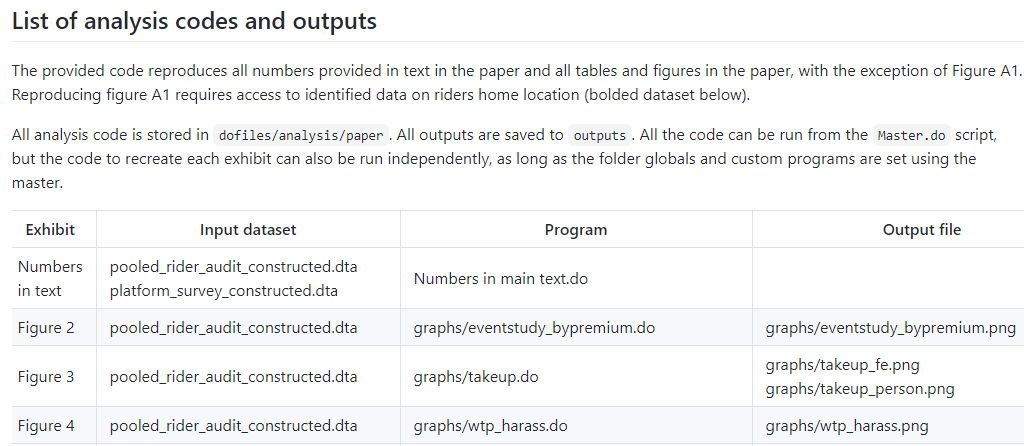
\includegraphics{examples/README.png}


\includegraphics[width=0.46\textwidth,height=\textheight]{examples/home.png}
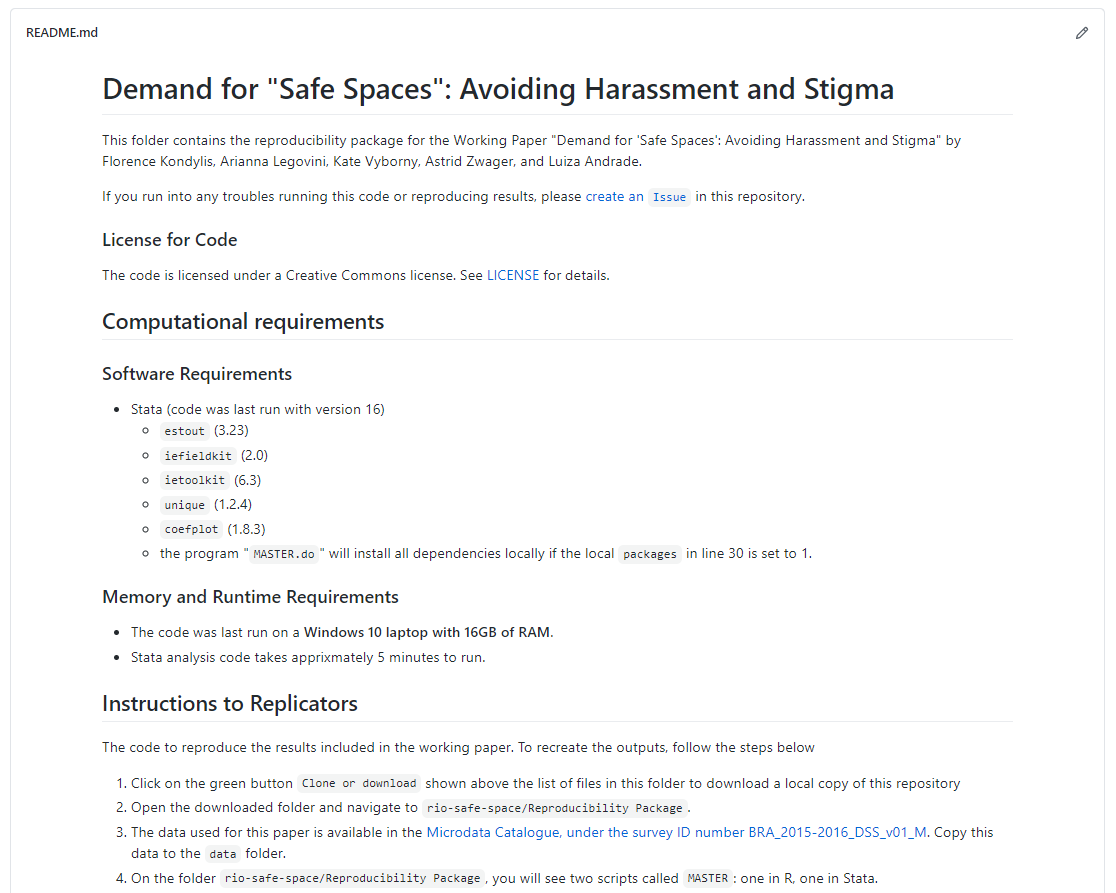
\includegraphics[width=0.53\textwidth,height=\textheight]{examples/github.png}

\begin{quote}
The GitHub repository can be accessed at \url{https://github.com/worldbank/rio-safe-space}.
\end{quote}
\end{ex}

\hypertarget{looking-ahead-7}{%
\section*{Looking ahead}\label{looking-ahead-7}}
\addcontentsline{toc}{section}{Looking ahead}

This chapter described the culmination of all the efforts in data acquisition, cleaning, processing, and analyzing --
the production of materials to share with the world
that answer a scientific or policy question in a way that has
never been done before.
The figure included in this chapter provides an overview
of all the outputs created by this stage.
Making sure that everything you discovered and created
is as broadly available and as easy to use as possible
is the last step in producing scientific evidence from original data.
This is the purpose of all the rigor, organization, and documentation
we encourage and detail at every step of the process:
since all your research materials are
continuously organized, shareable, secure, documented, and readable,
they are both valuable to you and others and easy to provide access to.

\begin{figure}
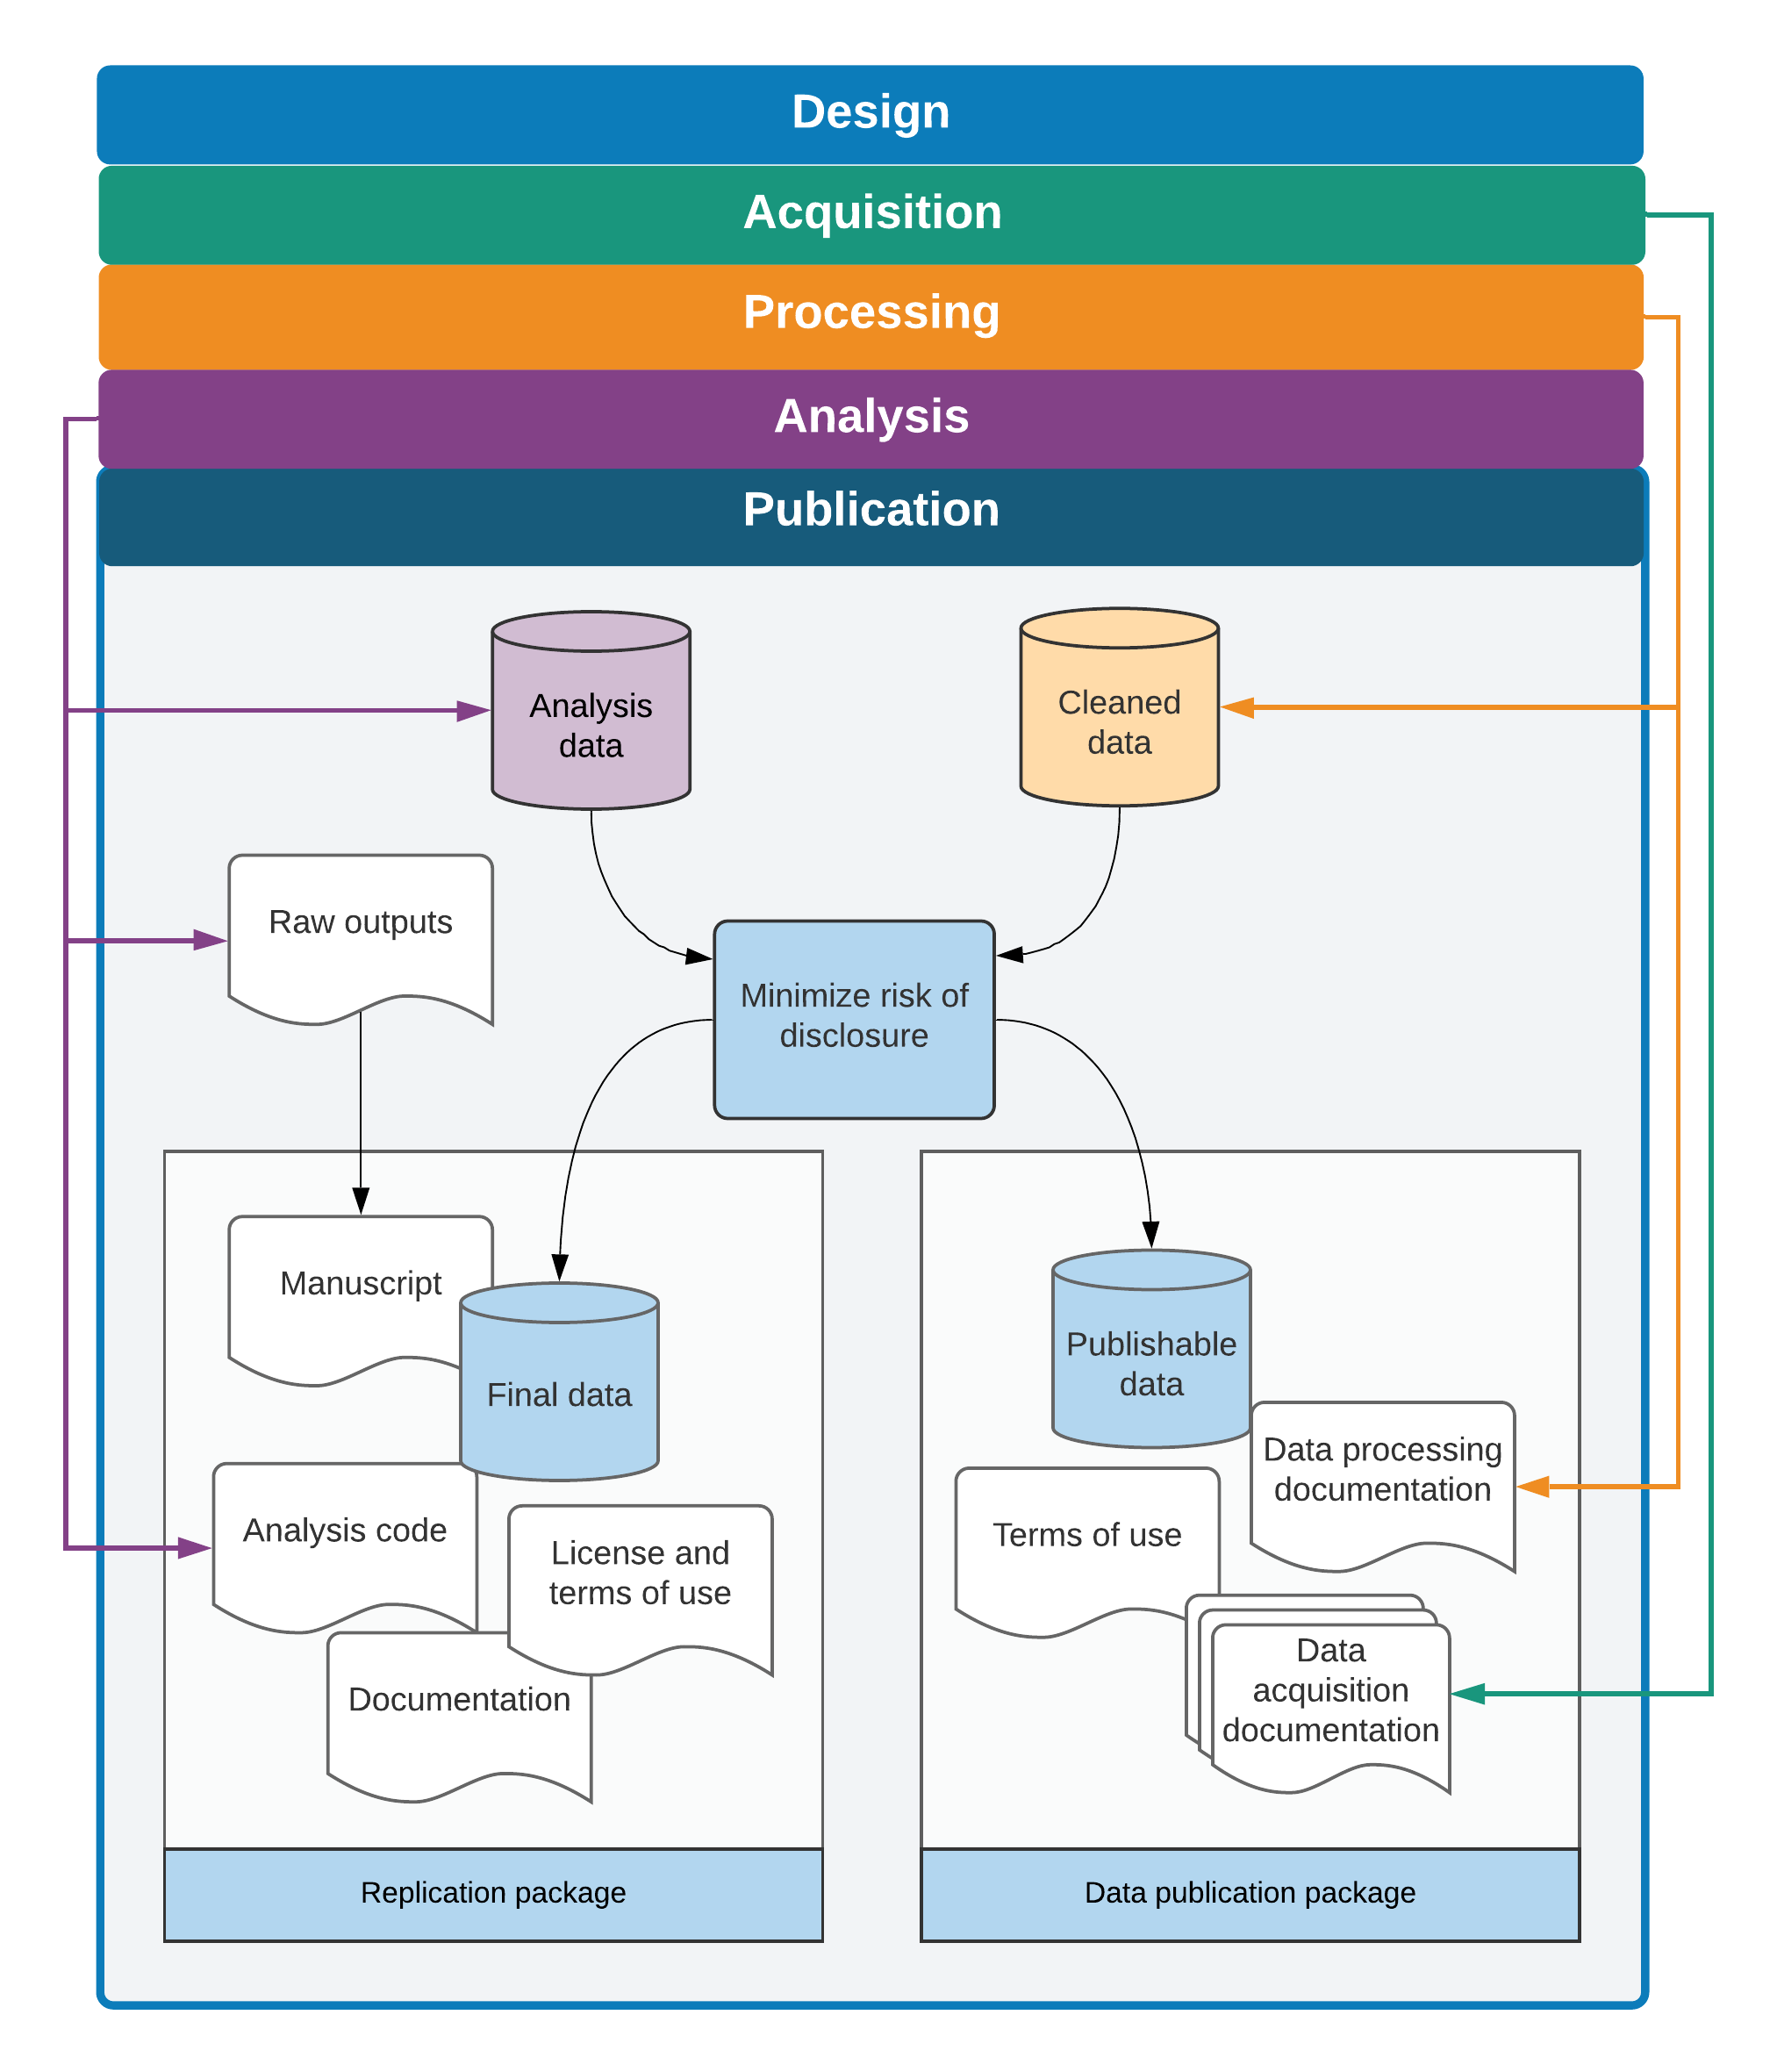
\includegraphics[width=28.12in]{diagrams/Publication} \caption{Publication tasks and outputs}\label{fig:unnamed-chunk-48}
\end{figure}

\hypertarget{bringing-it-all-together}{%
\chapter{Bringing it all together}\label{bringing-it-all-together}}

We hope you have enjoyed \emph{Development Research in Practice: The DIME Analytics Data Handbook}.
Our aim was to teach you to handle data more efficiently, effectively, and ethically.
We laid out a complete vision of the tasks of a modern researcher,
from planning a project's data governance to publishing code and data
to accompany a research product.
We have tried to set the text up as a resource guide
so that you will always be able to return to it
as your work requires you to become progressively more familiar
with each of the topics included in the guide.

We started the book with a discussion of
credibility, transparency, and reproducibility in research:
an overarching idea that your work should always be
accessible and available to others, both within and outside your team.
We then discussed the current research work environment,
which necessitates cooperation with a diverse group of collaborators
using modern approaches to computing technology.
We outlined methods for planning your data work
and creating basic documentation for data,
so that multiple data sources can be linked without error
and so that you can map the structure of your data
to your research design.
We discussed how to implement reproducible routines for sampling and randomization,
and to analyze statistical power and use randomization inference.

We detailed modern data acquisition methods and frameworks,
including data licensing, data ownership,
electronic data collection, and data security.
We provided a detailed workflow for data cleaning and processing,
emphasizing tidy data, quality control, privacy protection, and documentation.
We discuss the creation of derived indicators and analysis outputs,
and give an overview of the workflow required to move these results
to publication -- no matter the format of your work --
as well as tools and practices for making this work publicly accessible.
Throughout, we emphasized that data work is a ``social process'',
involving multiple team members with different roles and technical abilities.
This mindset and workflow, from top to bottom,
outline the tasks and responsibilities
that are fundamental to doing credible research.

However, as you probably noticed, the text itself provides
just enough detail to get you started:
an understanding of the purpose and function of each of the core research steps.
The references and resources get into the details
of how you will realistically implement these tasks:
from DIME Wiki pages detail specific code conventions
and field procedures that our team considers best practices,
to the theoretical papers that will help you figure out
how to handle the unique cases you will undoubtedly encounter.
We hope you will keep the book on your desk
(or the PDF on your desktop)
and come back to it anytime you need more information.
We wish you all the best in your work
and will love to hear any input you have on ours!
You can share your comments and suggestion on this book through
\url{https://worldbank.github.io/dime-data-handbook}.

\begin{figure}
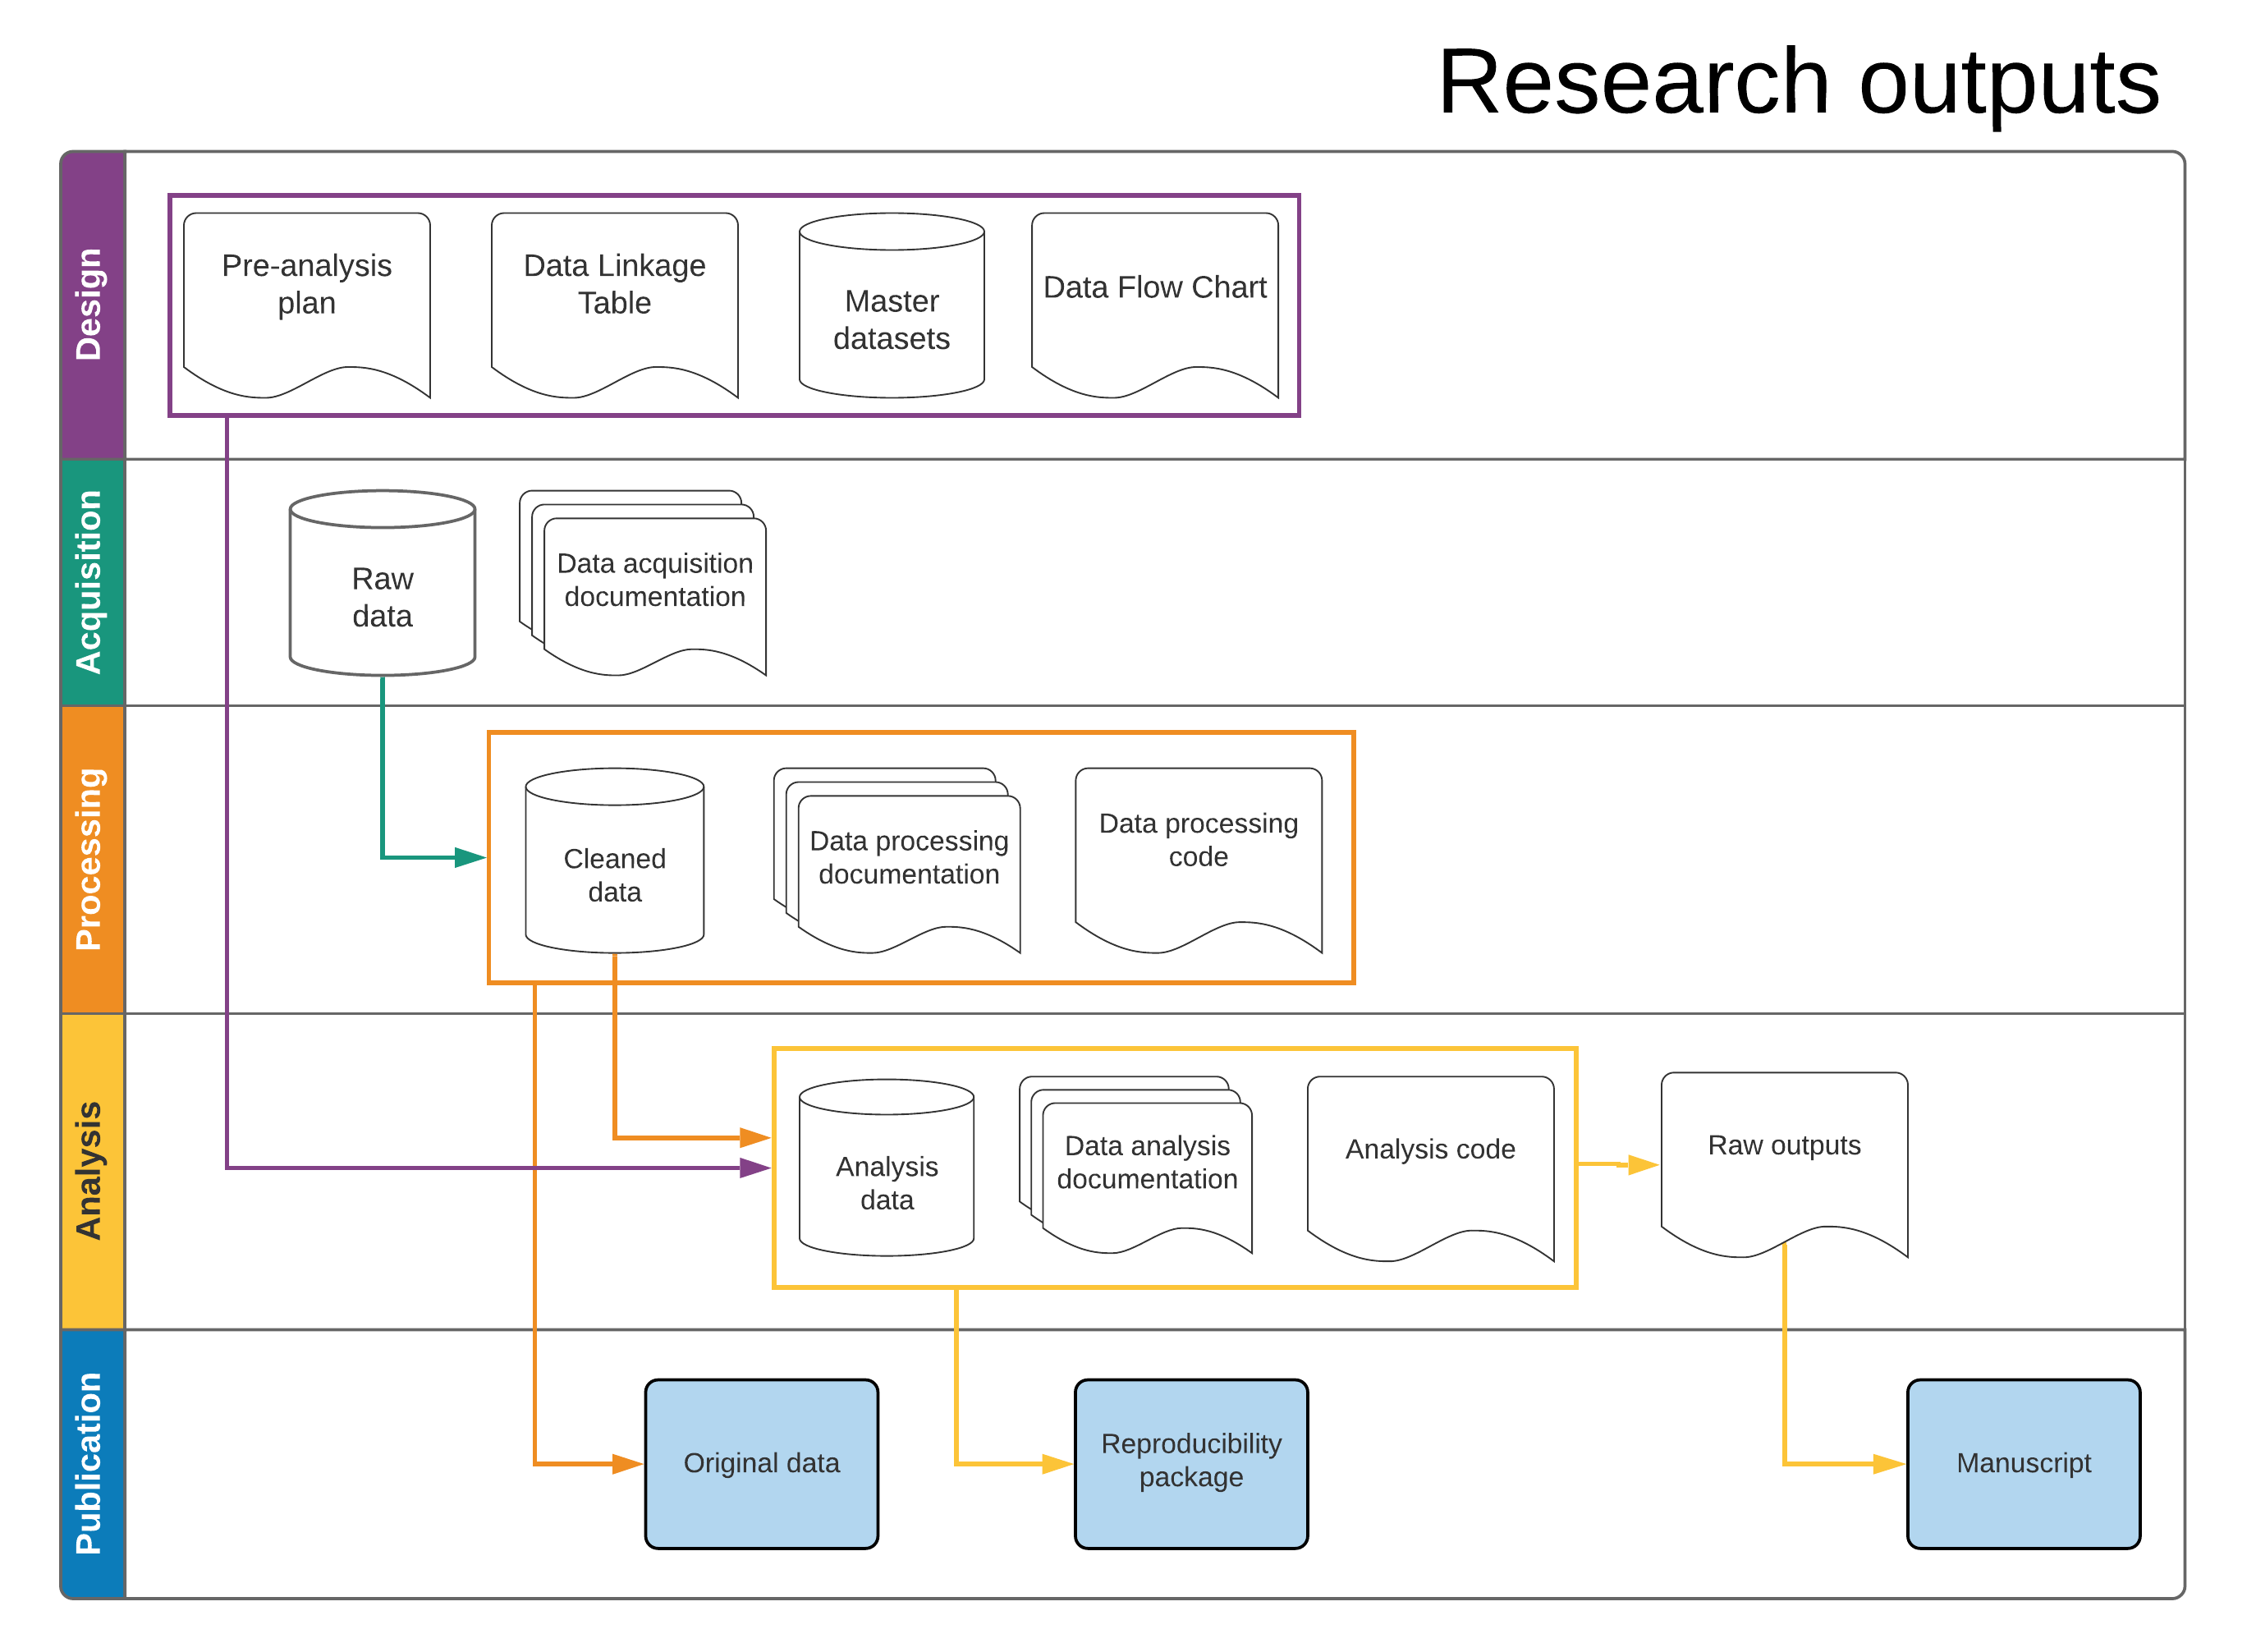
\includegraphics[width=31.93in]{diagrams/Conclusion} \caption{Research data work outputs}\label{fig:unnamed-chunk-49}
\end{figure}

\hypertarget{appendix-appendix}{%
\appendix}


\hypertarget{coding}{%
\chapter{The DIME Analytics Coding Guide}\label{coding}}

Most academic programs that prepare students for a career
in the type of work discussed in this book
spend a disproportionately small amount of time
teaching their students coding skills
in relation to the share of their professional time
they will spend writing code
in their first few years after they graduate.
Recent masters-level graduates joining our team
have shown very good theoretical knowledge
while requiring a lot of training in practical skills.
To us, this is like an architecture graduate having learned
how to sketch, describe, and discuss
the concepts and requirements of a new building very well --
but without the technical ability
to contribute to a blueprint following professional standards
that can be used and understood by others.
The reasons for this are a topic for another book,
but in today's data-driven world,
people working in quantitative development research
must be proficient collaborative programmers,
and that includes more than being able to compute correct numbers.

This appendix begins with a section on some general and language-agnostic
principles on how to write ``good'' code.
Good code is code that both generates correct results \emph{and}
is easily read and adapted by other professionals.
The second section in this appendix contains instructions
on how to access and use the code examples in this book.
The last section contains the DIME Analytics Stata Style Guide.
Widely accepted and used style guides are common in most programming languages,
but we have never found a sufficiently encompassing style guide for Stata.
We created this style guide having in mind practices that,
in our experience, greatly improve the quality
of research projects coded in Stata.
We hope that this guide can help increase the emphasis
given to using, improving, sharing, and standardizing code style
among the Stata community.
We believe these resources can help anyone write more understandable code,
and how you, like an architect,
can create a blueprint that can be understood and used
by everyone in your trade.

\hypertarget{writing-good-code}{%
\section*{Writing good code}\label{writing-good-code}}
\addcontentsline{toc}{section}{Writing good code}

``Good'' code has two elements:
(1) it is correct, in that it doesn't produce any errors
and its outputs are the objects intended,
and (2) it is useful and comprehensible
to someone who hasn't seen it before
(or even someone who has, weeks, months, or years later).
Many researchers have only been trained to code correctly.
But we believe that when your code runs on your computer
and you get the desired results,
you are only half-done writing \emph{good} code.
Good code is easy to read and replicate,
making it easier to spot mistakes.
Good code reduces sampling, randomization, and cleaning errors.
Good code can easily be reviewed by others
before it's published and can be re-used afterwards.
We always tell people to ``code as if a stranger is reading it''.

You should think of good code in terms of three major elements:
\textbf{structure}, \textbf{syntax}, and \textbf{style}.
The \textbf{structure} is the environment
and file organization your code lives in:
good structure means that it is easy to find individual pieces of code,
within and across files,
that correspond to specific tasks and outputs.
It also means that functional code blocks
are sufficiently independent from each other
such that they can be shuffled around, repurposed,
and even deleted without affecting the execution of other portions.
The \textbf{syntax} is the literal language of your code.
Good syntax means that your code is readable
in terms of how its mechanics implement ideas --
it should not require arcane reverse-engineering
to figure out what a code chunk is trying to do.
It should use common commands in a generally accepted way
so others can easily follow and reconstruct your intentions.
Finally, \textbf{style} is the way
that the non-functional elements of your code convey its purpose.
Elements like spacing, indentation,
and naming conventions (or lack thereof)
can make your code much more
(or much less) accessible to someone
who is reading it for the first time
and needs to understand it quickly and accurately.

One key tool for writing good code is using help documentation.
Whether or not you are new to the programming language you are using
-- Stata, R, Python, or one of the many others --
you should constantly revisit help files for the most common commands.
Often you will learn they can do something you never realized.
We cannot emphasize enough how important it is
that you get into the habit of reading help files,
especially for commands you are very familiar with.
Most of us have a help file window open at all times.
Similarly, you will always run into commands or uses of commands that
you have not seen before or whose functionality you do not remember.
Every time that happens,
you should look up the help file for that command.
We often encounter the conception that help files are only for beginners.
We could not disagree with that conception more.
The only way to get better at the programming language you use
is to constantly read help files.

\hypertarget{using-the-code-examples-in-this-book}{%
\section*{Using the code examples in this book}\label{using-the-code-examples-in-this-book}}
\addcontentsline{toc}{section}{Using the code examples in this book}

Providing some standardization for Stata code style
is also a goal of our team.
Stata is one of several programming languages used at DIME,
but since few high-quality resources based on Stata exist
relative to its importance and frequency of use,
we decided to use Stata for the examples in this book.
This book includes several code blocks
where we demonstrate a good code execution
of some of the most common tasks in data work.
We have ensured that each code block runs independently,
is well-formatted,
and uses built-in commands as much as possible.
We hope that these snippets will provide a foundation for your code style.
We try to comment code examples generously (as you should),
and you should reference Stata help files by writing \texttt{help\ {[}command{]}}
whenever you do not understand the command that is being used.
For example, if you are not familiar with \texttt{isid},
then write \texttt{help\ isid},
and the help file for the command \texttt{isid} will open.
You should do this even if you know \texttt{isid}
but has not read the help file for that command in a while,
as there is always something new to learn.

In the book, code examples are presented like the following:

\begin{Shaded}
\begin{Highlighting}[numbers=left,,]
\NormalTok{* Load the auto dataset}
    \KeywordTok{sysuse}\NormalTok{ auto.dta , }\KeywordTok{clear}

\NormalTok{* Run a simple regression}
    \KeywordTok{reg}\NormalTok{ price mpg rep78 headroom , coefl}

\NormalTok{* Transpose and }\KeywordTok{store}\NormalTok{ the output}
    \FunctionTok{matrix}\NormalTok{ results = }\FunctionTok{r}\NormalTok{(}\KeywordTok{table}\NormalTok{)'}

\NormalTok{* Load the results into }\DecValTok{memory}
    \KeywordTok{clear}
    \KeywordTok{svmat}\NormalTok{ results , n(col)}
\end{Highlighting}
\end{Shaded}

You can access the raw code used in examples in this book in several ways.
We use GitHub to version control all the content of this book,
including the code examples.
To see the code examples on GitHub, go to
\url{https://github.com/worldbank/dime-data-handbook/tree/master/code}.
We only use Stata's built-in datasets in our code examples,
so you do not need to download any data.
If you have Stata installed on your computer,
then you will already have the data files used in the code.

A less technical way to access the code
is to click the individual file in the URL above, then click
the button that says \textbf{Raw}.
You will then get to a page that looks like the one at
\url{https://raw.githubusercontent.com/worldbank/dime-data-handbook/master/code/code.do}.
There, you can copy the code
from your browser window to your do-file editor with the formatting intact.
This method is only practical for a single file at a time.
If you want to download all code used in this book, you can do that at
\url{https://github.com/worldbank/dime-data-handbook/archive/master.zip}.
That link downloads a \texttt{.zip} file
with all the content used in writing this book,
including the LaTeX code used for the book itself.
After extracting the .zip-file you will find all the code in a folder called \texttt{/code/}.

While we use built-in commands as much as possible in this book,
we point to user-written commands when they provide important new functionality.
In particular, we point to two suites of Stata commands developed by DIME Analytics,
\texttt{ietoolkit}\footnote{\url{https://dimewiki.worldbank.org/ietoolkit}}
and \texttt{iefieldkit},\footnote{\url{https://dimewiki.worldbank.org/iefieldkit}}
which DIME Analytics wrote to standardize
core data collection, management, and analysis workflows.

When you encounter code that employs user-written commands,
you will not be able to run them or read their help files
until you have installed the commands.
The most common place to distribute user-written commands for Stata
is the Boston College Statistical Software Components (SSC) archive.\footnote{\url{https://ideas.repec.org/s/boc/bocode.html}}
The user-written commands in our code example are all from the SSC archive.
So, if your installation of Stata does not recognize a command in our code, for example
\texttt{randtreat}, then type \texttt{ssc\ install\ randtreat} in Stata.

Some commands on SSC are distributed in packages.
This is the case, for example, of \texttt{ieboilstart}.
That means that you will not be able to install it using \texttt{ssc\ install\ ieboilstart}.
If you do, Stata will suggest that you instead use \texttt{findit\ ieboilstart},
which will search SSC (among other places) and see if there is a
package that contains a command called \texttt{ieboilstart}.
Stata will find \texttt{ieboilstart} in the package \texttt{ietoolkit},
so to use this command you will type \texttt{ssc\ install\ ietoolkit} in Stata instead.

We understand that it can be confusing to work with packages for first time,
but this is the best way to set up your Stata installation to benefit from other
people's work that has been made publicly available.
Once you get used to installing commands like this it will not be confusing at all.
All code with user-written commands, furthermore, is best written when it installs such commands
at the beginning of the master do-file,
so that the user does not have to search for packages manually.

\hypertarget{resources}{%
\chapter{DIME Analytics Resource Directory}\label{resources}}

The resources listed in this appendix are mentioned elsewhere in the chapters of this book,
and this appendix includes them all in one place for easy reference.
All these resources are made public under generous open-source licenses.
This means that you are free to use, reuse, and adapt these resources for any purpose as you see fit,
so long as you include an appropriate citation.

\hypertarget{public-resources-and-tools}{%
\section*{Public resources and tools}\label{public-resources-and-tools}}
\addcontentsline{toc}{section}{Public resources and tools}

\textbf{DIME Wiki.} One-stop shop for impact evaluation research solutions. The DIME Wiki is a resource focused on practical implementation guidelines rather than theory, open to the public, easily searchable, suitable for users of varying levels of expertise, up-to-date with the latest technological advances in electronic data collection, and curated by a vibrant network of editors with expertise in the field.
Hosted at \url{https://dimewiki.worldbank.org}.

\textbf{Stata Visual Library.} A curated, easy-to-browse selection of graphs created in Stata. Clicking on each graph reveals the source code, to allow for easy replication.
Hosted at \url{https://worldbank.github.io/stata-visual-library/}.

\textbf{R Econ Visual Library.} A curated, easy-to-browse selection of graphs created in R. Clicking on each graph reveals the source code, to allow for easy replication.
Hosted at \url{https://worldbank.github.io/r-econ-visual-library/}.

\textbf{DIME Analytics Research Standards.} A repository outlining DIME's public commitments to research ethics, transparency, reproducibility, data security and data publication, along with supporting tools and resources.
Hosted at \url{https://github.com/worldbank/dime-standards}.

\hypertarget{flagship-training-courses}{%
\section*{Flagship training courses}\label{flagship-training-courses}}
\addcontentsline{toc}{section}{Flagship training courses}

\textbf{Manage Successful Impact Evaluations (MSIE).}
DIME Analytics' flagship training is a week-long annual course,
held in person in Washington, DC. MSIE is intended to improve the skills and knowledge of impact evaluation (IE) practitioners,
familiarizing them with critical issues in IE implementation,
recurring challenges, and cutting-edge technologies.
The course consists of lectures and hands-on sessions.
Through small group discussions and interactive computer lab sessions,
participants work together to apply what they've learned and have a first-hand opportunity to develop skills.
Hands-on sessions are offered in parallel tracks,
with different options based on software preferences and skill level.
The course materials are available at \url{https://osf.io/h4d8y/}.

\textbf{Manage Successful Impact Evaluation Surveys (MSIES).}
A fully virtual course, in which participants learn the workflow for primary data collection.
The course covers best practices at all stages of the survey workflow,
from planning to piloting instruments and monitoring data quality once fieldwork begins.
There is a strong focus throughout on research ethics and reproducible workflows.
The course uses a combination of virtual lectures,
case studies, readings, and hands-on exercises.
The course materials are available at \url{https://osf.io/resya/}.

\textbf{Research Assistant Onboarding Course.}
This course is designed to familiarize Research Assistants and Research Analysts with DIME's standards for data work.
By the end of the course's six sessions,
participants have the tools and knowledge to implement best practices for transparent and reproducible research.
The course focuses on how to set up a collaborative workflow for code,
datasets, and research outputs.
Most content is platform-independent and software-agnostic,
but participants are expected to be familiar with statistical software.
The course materials are available at \url{https://osf.io/qtmdp}.

\textbf{Introduction to R for Advanced Stata Users.}
This course is an introduction to the R programming language,
building upon knowledge of Stata. The course focuses on common tasks in development research,
related to descriptive analysis, data visualization, data processing, and geospatial data work.
Materials available at \url{https://osf.io/nj6bf}.

\textbf{DIME Analytics Trainings.}
DIME Analytics' home on the Open Science Framework,
with links to materials for all past courses and technical trainings.
Visit \url{https://osf.io/wzjtk} to explore the materials.

\hypertarget{software-tools-and-trainings}{%
\section*{Software tools and trainings}\label{software-tools-and-trainings}}
\addcontentsline{toc}{section}{Software tools and trainings}

\textbf{ietoolkit.} Suite of Stata commands to routinize common tasks for data management and impact evaluation analysis.
Developed at \url{https://github.com/worldbank/ietoolkit}.

\textbf{iefieldkit.} Suite of Stata commands to routinize and document common tasks in primary data collection.
Developed at \url{https://github.com/worldbank/iefieldkit}.

\textbf{DIME Analytics GitHub Trainings and Resources.} A GitHub repository containing all the GitHub training materials and
resources developed by DIME Analytics.
The trainings follow DIME's model for organizing research teams on GitHub,
and are designed for face-to-face delivery,
but materials are shared so that they may be used and adapted by others.
Hosted at \url{https://github.com/worldbank/dime-github-trainings}.

\textbf{DIME Analytics LaTeX Training.} A user-friendly guide to getting started with LaTeX.
Exercises provide opportunities to practice creating appendices,
exporting tables from R or Stata to LaTeX,
and formatting tables in LaTeX.
Available at \url{https://github.com/worldbank/DIME-LaTeX-Templates}.

\hypertarget{design}{%
\chapter{Research design for impact evaluation}\label{design}}

\emph{Development Research in Practice} focuses on tools, workflows, and practical
guidance for implementing research projects.
While not central to the content of this book,
We think it is essential for all research team members
-- including field staff and research assistants --
to understand research design,
and specifically how research design choices impact data work.
Without going into too much technical detail,
as there are many excellent resources on impact evaluation design,
this appendix presents a brief overview
of the most common causal inference methods,
focusing on implications for data structure and analysis.
This appendix is intended to be a reference,
especially for junior team members,
to obtain an understanding of the way in which each
causal inference method constructs treatment and control groups,
the data structures needed to estimate the corresponding effects,
and specific code tools designed for each method.

It is essential for the research team members who will do the data work
to understand the study design, for several reasons.
If you do not know how to calculate the correct estimator for your study,
you will not be able to assess the statistical power of your research design.
You will also be unable to make decisions in the field
when you inevitably have to allocate scarce resources
between tasks like maximizing sample size
and ensuring follow-up with specific individuals.
You will save time by understanding the way your data needs to be organized
to produce meaningful analytics throughout your projects.
Just as importantly, familiarity with each of these approaches
will allow you to keep your eyes open for research opportunities:
many of the most interesting projects occur because people in the field
recognize the opportunity to implement one of these methods
in response to an unexpected event.

This appendix is split into two sections.
The first covers causal inference methods
in experimental and quasi-experimental research designs.
The second discusses how to measure treatment effects and structure data for specific methods,
including cross-sectional randomized control trials, difference-in-difference designs,
regression discontinuity, instrumental variables, matching, and synthetic controls.

\hypertarget{understanding-causality-inference-and-identification}{%
\section*{Understanding causality, inference, and identification}\label{understanding-causality-inference-and-identification}}
\addcontentsline{toc}{section}{Understanding causality, inference, and identification}

When we are discussing the types of inputs -- ``treatments'' -- commonly referred to as
``programs'' or ``interventions'', we are typically attempting to obtain estimates
of program-specific \textbf{treatment effects}.
These are the changes in outcomes attributable to the treatment.\footnote{Abadie and Cattaneo (\protect\hyperlink{ref-abadie2018econometric}{2018})}
\index{treatment effect}
The primary goal of research design is to establish \textbf{causal identification} for an effect.
Causal identification means establishing that a change in an input directly altered an outcome.
\index{identification}
When a study is well-identified, then we can say with confidence
that our estimate of the treatment effect would,
with an infinite amount of data,
give us a precise estimate of that treatment effect.
Under this condition, we can proceed to draw evidence from the limited samples we have access to,
using statistical techniques to express the uncertainty of not having infinite data.
Without identification, we cannot say that the estimate would be accurate,
even with unlimited data, and therefore cannot attribute it to the treatment
in the small samples that we typically have access to.
More data is not a substitute for a well-identified experimental design.
Therefore it is important to understand how exactly your study
identifies its estimate of treatment effects,
so you can calculate and interpret those estimates appropriately.

All the study designs we discuss here use the potential outcomes framework\footnote{Athey and Imbens (\protect\hyperlink{ref-athey2017state}{2017}\protect\hyperlink{ref-athey2017state}{b})}
to compare a group that received some treatment to another, counterfactual group.
Each of these approaches can be used in two types of designs:
\textbf{experimental} designs, in which the research team
is directly responsible for creating the variation in treatment,
and \textbf{quasi-experimental} designs, in which the team
identifies a ``natural'' source of variation and uses it for identification.
Neither type is implicitly better or worse,
and both types are capable of achieving causal identification in different contexts.

\hypertarget{estimating-treatment-effects-using-control-groups}{%
\subsection*{Estimating treatment effects using control groups}\label{estimating-treatment-effects-using-control-groups}}
\addcontentsline{toc}{subsection}{Estimating treatment effects using control groups}

The key assumption behind estimating treatment effects is that every
person, facility, or village (or whatever the unit of intervention is)
has two possible states: their outcomes if they do not receive some treatment
and their outcomes if they do receive that treatment.
Each unit's treatment effect is the individual difference between these two states,
and the \textbf{average treatment effect (ATE)} is the average of all
individual differences across the potentially treated population.
\index{average treatment effect}
This is the parameter that most research designs attempt to estimate,
by establishing a \textbf{counterfactual}\footnote{\textbf{Counterfactual:} A statistical description of what would have happened to specific individuals in an alternative scenario,
  for example, a different treatment assignment outcome. for the treatment group against which outcomes can be directly compared.}\index{counterfactual}
There are several resources that provide more or less mathematically intensive
approaches to understanding how various methods do this.
\emph{Impact Evaluation in Practice}\footnote{Gertler et al. (\protect\hyperlink{ref-gertler2016impact}{2016})}
is a strong general guide to these methods.
\emph{Causal Inference}\footnote{Hernán and Robins (\protect\hyperlink{ref-hernan2010causal}{2010})} and
\emph{Causal Inference: The Mixtape}\footnote{Cunningham (\protect\hyperlink{ref-cunningham2018causal}{2018})}
provides more detailed mathematical approaches to the tools.
\emph{Mostly Harmless Econometrics}\footnote{Angrist and Pischke (\protect\hyperlink{ref-angrist2008mostly}{2008})}
and \emph{Mastering Metrics}\footnote{Angrist and Pischke (\protect\hyperlink{ref-angrist2014mastering}{2014})}
are excellent resources on the statistical principles behind all econometric approaches.

Intuitively, the problem is as follows: we can never observe the same unit
in both their treated and untreated states simultaneously,
so measuring and averaging these effects directly is impossible.\footnote{Rubin (\protect\hyperlink{ref-rubin2003basic}{2003})}
Instead, we typically make inferences from samples.
\textbf{Causal inference} methods are those in which we are able to estimate the
average treatment effect without observing individual-level effects,
but through some comparison of averages with a \textbf{control} group.
\index{causal inference}\index{control group}
Every research design is based on a way of comparing another set of observations --
the ``control'' observations -- against the treatment group.
They all work to establish that the control observations would have been
identical \emph{on average} to the treated group in the absence of the treatment.
Then, the mathematical properties of averages imply that the calculated
difference in averages is equivalent to the average difference:
exactly the parameter we are seeking to estimate.
Therefore, almost all designs can be accurately described
as a series of between-group comparisons.

Most of the methods that you will encounter rely on some variant of this strategy,
which is designed to maximize their ability to estimate the effect
of an average unit being offered the treatment you want to evaluate.
The focus on identification of the treatment effect, however,
means there are several essential features of causal identification methods
that are not common in other types of statistical and data science work.
First, the econometric models and estimating equations used
do not attempt to create a predictive or comprehensive model
of how the outcome of interest is generated.
Typically, causal inference designs are not interested in predictive accuracy,
and the estimates and predictions that they produce
will not be as good at predicting outcomes or fitting the data as other models.
Second, when control variables or other variables are used in estimation,
there is no guarantee that the resulting parameters are marginal effects.
They can only be interpreted as correlative averages,
unless there are additional sources of identification.
The models you will construct and estimate are intended to do exactly one thing:
to express the intention of your project's research design,
and to accurately estimate the effect of the treatment it is evaluating.
In other words, these models tell the story of the research design
in a way that clarifies the exact comparison being made between control and treatment.

\hypertarget{designing-experimental-and-quasi-experimental-research}{%
\subsection*{Designing experimental and quasi-experimental research}\label{designing-experimental-and-quasi-experimental-research}}
\addcontentsline{toc}{subsection}{Designing experimental and quasi-experimental research}

Experimental research designs explicitly allow the research team
to change the condition of the populations being studied,\footnote{\url{https://dimewiki.worldbank.org/Experimental_Methods}}
often in the form of government programs, NGO projects, new regulations,
information campaigns, and many more types of interventions.\footnote{Banerjee and Duflo (\protect\hyperlink{ref-banerjee2009experimental}{2009})}
The classic experimental causal inference method
is the \textbf{randomized control trial (RCT)}.\footnote{\url{https://dimewiki.worldbank.org/Randomized_Control_Trials}}\index{randomized control trials}
In randomized control trials, the treatment group is randomized --
that is, from an eligible population,
a random group of units are given the treatment.
Another way to think about these designs is how they establish the control group:
a random subset of units are \emph{not} given access to the treatment,
so that they may serve as a counterfactual for those who are.
A randomized control group, intuitively, is meant to represent
how things would have turned out for the treated group
if they had not been treated, and it is particularly effective at doing so
as evidenced by its broad credibility in fields ranging from clinical medicine to development.
Therefore RCTs are very popular tools for determining the causal impact
of specific programs or policy interventions,
as evidenced by the awarding of the 2019 Nobel Prize in Economics
to Abhijit Banerjee, Esther Duflo and Michael Kremer
``for their experimental approach to alleviating global poverty.''\footnote{NobelPrize.org (\protect\hyperlink{ref-nobel2019}{2020})}
However, there are many other types of interventions that are impractical or unethical
to effectively approach using an experimental strategy,
and therefore there are limitations to accessing ``big questions''
through RCT approaches.\footnote{Deaton (\protect\hyperlink{ref-deaton2009}{2009})}

Randomized designs all share several major statistical concerns.
The first is the fact that it is always possible to select a control group,
by chance, which is not in fact very similar to the treatment group.
This feature is called randomization noise, and all RCTs share the need to assess
how randomization noise may impact the estimates that are obtained.
(More detail on this later.)
Second, take-up and implementation fidelity are extremely important,
since programs will by definition have no effect
if the population intended to be treated
does not accept or does not receive the treatment.\footnote{See Jung and Hasan (\protect\hyperlink{ref-jung2016impact}{2016}) for an example.}
Loss of statistical power occurs quickly and is highly nonlinear:
70\% take-up or efficacy doubles the required sample, and 50\% quadruples it.\footnote{\url{https://blogs.worldbank.org/impactevaluations/power-calculations-101-dealing-with-incomplete-take-up}}
Such effects are also very hard to correct ex post,
since they require strong assumptions about the randomness or non-randomness of take-up.
Therefore a large amount of field time and descriptive work
must be dedicated to understanding how these effects played out in a given study,
and may overshadow the effort put into the econometric design itself.

\textbf{Quasi-experimental} research designs,\footnote{\url{https://dimewiki.worldbank.org/Quasi-Experimental_Methods}}
by contrast, are causal inference methods based on events not controlled by the research team.
Instead, they rely on ``experiments of nature'',
in which natural variation can be argued to approximate
the type of exogenous variation in treatment availability
that a researcher would attempt to create with an experiment.\footnote{DiNardo (\protect\hyperlink{ref-dinardo2016natural}{2016})}
Unlike carefully planned experimental designs,
quasi-experimental designs typically require the extra luck
of having access to data collected at the right times and places
to exploit events that occurred in the past,
or having the ability to collect data in a time and place
where an event that produces causal identification occurred or will occur.
Therefore, these methods often use either secondary data,
or they use primary data in a cross-sectional retrospective method,
including administrative data or other new classes of routinely-collected information.

Quasi-experimental designs therefore can access a much broader range of questions,
and with much less effort in terms of executing an intervention.
However, they require in-depth understanding of the precise events
the researcher wishes to address in order to know what data to use
and how to model the underlying natural experiment.
Additionally, because the population exposed
to such events is limited by the scale of the event,
quasi-experimental designs are often power-constrained.
Since the research team cannot change the population of the study
or the treatment assignment, power is typically maximized by ensuring
that sampling for data collection is carefully designed to match the study objectives
and that attrition from the sampled groups is minimized.

\hypertarget{obtaining-treatment-effects-from-specific-research-designs}{%
\section*{Obtaining treatment effects from specific research designs}\label{obtaining-treatment-effects-from-specific-research-designs}}
\addcontentsline{toc}{section}{Obtaining treatment effects from specific research designs}

\hypertarget{cross-sectional-designs}{%
\subsection*{Cross-sectional designs}\label{cross-sectional-designs}}
\addcontentsline{toc}{subsection}{Cross-sectional designs}

A cross-sectional research design is any type of study
that observes data in only one time period
and directly compares treatment and control groups.
This type of data is easy to collect and handle because
you do not need to track individuals across time.
If this point in time is after a treatment has been fully delivered,
then the outcome values at that point in time
already reflect the effect of the treatment.
If the study is experimental, the treatment and control groups are randomly constructed
from the population that is eligible to receive each treatment.
By construction, each unit's receipt of the treatment
is unrelated to any of its other characteristics
and the ordinary least squares (OLS) regression
of outcome on treatment, without any control variables,
is an unbiased estimate of the average treatment effect.

Cross-sectional designs can also exploit variation in non-experimental data
to argue that observed correlations do in fact represent causal effects.
This can be true unconditionally -- which is to say that something random,
such as winning the lottery, is a true random process and can tell you about the effect
of getting a large amount of money.\footnote{Imbens, Rubin, and Sacerdote (\protect\hyperlink{ref-imbens2001estimating}{2001})}
It can also be true conditionally -- which is to say that once the
characteristics that would affect both the likelihood of exposure to a treatment
and the outcome of interest are controlled for,
the process is as good as random:
like arguing that once risk preferences are taken into account,
exposure to an earthquake is unpredictable and post-event differences
are causally related to the event itself.\footnote{Callen (\protect\hyperlink{ref-callen2015catastrophes}{2015})}
For cross-sectional designs, what needs to be carefully maintained in data
is the treatment randomization process itself (whether experimental or not),
as well as detailed information about differences
in data quality and attrition across groups.\footnote{Athey and Imbens (\protect\hyperlink{ref-athey2017econometrics}{2017}\protect\hyperlink{ref-athey2017econometrics}{a})}
Only these details are needed to construct the appropriate estimator:
clustering of the standard errors is required at the level
at which the treatment is assigned to observations,
and variables which were used to stratify the treatment
must be included as controls (in the form of strata fixed effects).\footnote{\url{https://blogs.worldbank.org/impactevaluations/impactevaluations/how-randomize-using-many-baseline-variables-guest-post-thomas-barrios}}
\textbf{Randomization inference} can be used
to estimate the underlying variability in the randomization process.
\textbf{Balance checks}\footnote{\textbf{Balance checks:} Statistical tests of the similarity of treatment and control groups.}
are often reported as evidence of an effective randomization,
and are particularly important when the design is quasi-experimental
(since then the randomization process cannot be simulated explicitly).
However, controls for balance variables are usually unnecessary in RCTs,
because it is certain that the true data-generating process
has no correlation between the treatment and the balance factors.\footnote{\url{https://blogs.worldbank.org/impactevaluations/should-we-require-balance-t-tests-baseline-observables-randomized-experiments}}

Analysis is typically straightforward \emph{once you have a strong understanding of the randomization}.
A typical analysis will include a description of the sampling and randomization results,
with analyses such as summary statistics for the eligible population,
and balance checks for randomization and sample selection.
The main results will usually be a primary regression specification
(with multiple hypotheses\footnote{See Armand et al. (\protect\hyperlink{ref-armand2017public}{2017}) for an example.}
appropriately adjusted for),
and additional specifications with adjustments for non-response, balance, and other potential contamination.
Robustness checks might include randomization-inference analysis or other placebo regression approaches.
There are a number of user-written code tools that are also available
to help with the complete process of data analysis,
including to analyze balance\footnote{\url{https://dimewiki.worldbank.org/iebaltab}}
and to visualize treatment effects.\footnote{\url{https://dimewiki.worldbank.org/iegraph}}
Extensive tools and methods for analyzing selective non-response are available.\footnote{\url{https://blogs.worldbank.org/impactevaluations/dealing-attrition-field-experiments}}

\hypertarget{difference-in-differences}{%
\subsection*{Difference-in-differences}\label{difference-in-differences}}
\addcontentsline{toc}{subsection}{Difference-in-differences}

Where cross-sectional designs draw their estimates of treatment effects
from differences in outcome levels in a single measurement,
\textbf{differences-in-differences}\footnote{\url{https://dimewiki.worldbank.org/Difference-in-Differences}}
designs (abbreviated as DD, DiD, diff-in-diff, and other variants)
estimate treatment effects from \emph{changes} in outcomes
between two or more rounds of measurement.
\index{difference-in-differences}
In these designs, three control groups are used --
the baseline level of treatment units,
the baseline level of non-treatment units,
and the endline level of non-treatment units.\footnote{Torres-Reyna (\protect\hyperlink{ref-torres2015}{2015})}
The estimated treatment effect is the excess growth
of units that receive the treatment, in the period they receive it:
calculating that value is equivalent to taking
the difference in means at endline and subtracting
the difference in means at baseline
(hence the singular ``difference-in-differences'').\footnote{McKenzie (\protect\hyperlink{ref-mckenzie2012beyond}{2012})}
The regression model includes a control variable for treatment assignment,
and a control variable for time period,
but the treatment effect estimate corresponds to
an interaction variable for treatment and time:
it indicates the group of observations for which the treatment is active.
This model depends on the assumption that,
in the absense of the treatment,
the outcome of the two groups would have changed at the same rate over time,
typically referred to as the \textbf{parallel trends} assumption.\footnote{\url{https://blogs.worldbank.org/impactevaluations/often-unspoken-assumptions-behind-difference-difference-estimator-practice}}
Experimental approaches satisfy this requirement in expectation,
but a given randomization should still be checked for pre-trends
as an extension of balance checking.\footnote{\url{https://blogs.worldbank.org/impactevaluations/revisiting-difference-differences-parallel-trends-assumption-part-i-pre-trend}}
There are two main types of data structures for differences-in-differences:
\textbf{repeated cross-sections} and \textbf{panel data}.
In repeated cross-sections, each successive round of data collection contains a random sample
of observations from the treated and untreated groups;
as in cross-sectional designs, both the randomization and sampling processes
are critically important to maintain alongside the data.
In panel data structures, we attempt to observe the exact same units
in different points in time, so that we see the same individuals
both before and after they have received treatment (or not).\footnote{\url{https://blogs.worldbank.org/impactevaluations/what-are-we-estimating-when-we-estimate-difference-differences}}
This allows each unit's baseline outcome (the outcome before the intervention) to be used
as an additional control for its endline outcome,
which can provide large increases in power and robustness.\footnote{\url{https://blogs.worldbank.org/impactevaluations/another-reason-prefer-ancova-dealing-changes-measurement-between-baseline-and-follow}}
When tracking individuals over time for this purpose,
maintaining sampling and tracking records is especially important,
because attrition will remove that unit's information
from all points in time, not just the one they are unobserved in.
Panel-style experiments therefore require a lot more effort in field work
for studies that use original data.\footnote{Torres-Reyna (\protect\hyperlink{ref-torres2007}{2007})}
Since baseline and endline may be far apart in time,
it is important to create careful records during the first round
so that follow-ups can be conducted with the same subjects,
and attrition across rounds can be properly taken into account.\footnote{\url{https://blogs.worldbank.org/impactevaluations/dealing-attrition-field-experiments}}

As with cross-sectional designs, difference-in-differences designs are widespread.
Therefore there exist a large number of standardized tools for analysis.
Our \texttt{ietoolkit} Stata package includes the \texttt{ieddtab} command
which produces standardized tables for reporting results.\footnote{\url{https://dimewiki.worldbank.org/ieddtab}}
For more complicated versions of the model
(and they can get quite complicated quite quickly),
you can use an online dashboard to simulate counterfactual results.\footnote{\url{https://blogs.worldbank.org/impactevaluations/econometrics-sandbox-event-study-designs-co}}
As in cross-sectional designs, these main specifications
will always be accompanied by balance checks (using baseline values),
as well as randomization, selection, and attrition analysis.
In trials of this type, reporting experimental design and execution
using the CONSORT style is common in many disciplines
and will help you to track your data over time.\footnote{Schulz, Altman, and Moher (\protect\hyperlink{ref-schulz2010consort}{2010})}

\hypertarget{regression-discontinuity}{%
\subsection*{Regression discontinuity}\label{regression-discontinuity}}
\addcontentsline{toc}{subsection}{Regression discontinuity}

\textbf{Regression discontinuity (RD)} designs exploit sharp breaks or limits
in policy designs to separate a single group of potentially eligible recipients
into comparable groups of individuals who do and do not receive a treatment.\footnote{\url{https://dimewiki.worldbank.org/Regression_Discontinuity}}
These designs differ from cross-sectional and diff-in-diff designs
in that the group eligible to receive treatment is not defined directly,
but instead created during the treatment implementation.
\index{regression discontinuity}
In an RD design, there is typically some program or event
that has limited availability due to practical considerations or policy choices
and is therefore made available only to individuals who meet a certain threshold requirement.
The intuition of this design is that there is an underlying \textbf{running variable}
that serves as the sole determinant of access to the program,
and a strict cutoff determines the value of this variable at which eligibility stops.\footnote{Imbens and Lemieux (\protect\hyperlink{ref-imbens2008regression}{2008})}\index{running variable}
Common examples are test score thresholds and income thresholds.\footnote{\url{https://blogs.worldbank.org/impactevaluations/regression-discontinuity-porn}}
The intuition is that individuals who are just above the threshold
will be very nearly indistinguishable from those who are just under it,
and their post-treatment outcomes are therefore directly comparable.\footnote{Lee and Lemieux (\protect\hyperlink{ref-lee2010regression}{2010})}
The key assumption here is that the running variable cannot be directly manipulated
by the potential recipients.
If the running variable is time (what is commonly called an ``event study''),
there are special considerations.\footnote{}Hausman and Rapson (\protect\hyperlink{ref-hausman2018regression}{2018})
Similarly, spatial discontinuity designs are handled a bit differently due to their multidimensionality.\footnote{\url{https://blogs.worldbank.org/impactevaluations/spatial-jumps}}

Regression discontinuity designs are, once implemented,
very similar in analysis to cross-sectional or difference-in-differences designs.
Depending on the data that is available,
the analytical approach will center on the comparison of individuals
who are narrowly on the inclusion side of the discontinuity,
compared against those who are narrowly on the exclusion side.\footnote{Cattaneo, Idrobo, and Titiunik (\protect\hyperlink{ref-cattaneo2019}{2019})}
The regression model will be identical to the matching research designs,
i.e., contingent on whether data has one or more time periods
and whether the same units are known to be observed repeatedly.
The treatment effect will be identified, however, by the addition of a control
for the running variable -- meaning that the treatment effect estimate
will only be applicable for observations in a small window around the cutoff:
in the lingo, the treatment effects estimated will be ``local'' rather than ``average''.
In the RD model, the functional form of the running variable control and the size of that window,
often referred to as the choice of \textbf{bandwidth} for the design,
are the critical parameters for the result.\footnote{Calonico et al. (\protect\hyperlink{ref-calonico2019regression}{2019})}
Therefore, RD analysis often includes extensive robustness checking
using a variety of both functional forms and bandwidths,
as well as placebo testing for non-realized locations of the cutoff.

In the analytical stage, regression discontinuity designs
often include a large component of visual evidence presentation.
These presentations help to suggest both the functional form
of the underlying relationship and the type of change observed at the discontinuity,
and help to avoid pitfalls in modeling that are difficult to detect with hypothesis tests.\footnote{Pischke (\protect\hyperlink{ref-pischke2018}{2018})}
Because these designs are so flexible compared to others,
there is an extensive set of commands that help assess
the efficacy and results from these designs under various assumptions.\footnote{Calonico, Cattaneo, and Titiunik (\protect\hyperlink{ref-calonico2014robust}{2014})}
These packages support the testing and reporting
of robust plotting and estimation procedures,
tests for manipulation of the running variable,
and tests for power, sample size, and randomization inference approaches
that will complement the main regression approach used for point estimates.

\hypertarget{instrumental-variables}{%
\subsection*{Instrumental variables}\label{instrumental-variables}}
\addcontentsline{toc}{subsection}{Instrumental variables}

\textbf{Instrumental variables (IV)} designs, unlike the previous approaches,
begin by assuming that the treatment delivered in the study in question is
linked to the outcome in a pattern such that its effect is not directly identifiable.
Instead, similar to regression discontinuity designs,
IV attempts to focus on a subset of the variation in treatment take-up
and assesses that limited window of variation that can be argued
to be unrelated to other factors.\footnote{Angrist and Krueger (\protect\hyperlink{ref-angrist2001instrumental}{2001})}
To do so, the IV approach selects an \textbf{instrument}
for the treatment status -- an otherwise-unrelated predictor of exposure to treatment
that affects the take-up status of an individual.\footnote{\url{https://dimewiki.worldbank.org/instrumental_variables}}
Whereas regression discontinuity designs are ``sharp'' --
treatment status is completely determined by which side of a cutoff an individual is on --
IV designs are ``fuzzy'', meaning that they do not completely determine
the treatment status but instead influence the \emph{probability} of treatment.

As in regression discontinuity designs,
the fundamental form of the regression
is similar to either cross-sectional or difference-in-differences designs.
However, instead of controlling for the instrument directly,
the IV approach typically uses the \textbf{two-stage-least-squares (2SLS)} estimator.\footnote{Bond (\protect\hyperlink{ref-bond2020}{2020})}
This estimator forms a prediction of the probability that the unit receives treatment
based on a regression against the instrumental variable.
That prediction will, by assumption, be the portion of the actual treatment
that is due to the instrument and not any other source,
and since the instrument is unrelated to all other factors,
this portion of the treatment can be used to assess its effects.
Unfortunately, these estimators are known
to have very high variances relative other methods,
particularly when the relationship between the instrument and the treatment is small.\footnote{Young (\protect\hyperlink{ref-young2017consistency}{2019})}
IV designs furthermore rely on strong but untestable assumptions
about the relationship between the instrument and the outcome.\footnote{Bound, Jaeger, and Baker (\protect\hyperlink{ref-bound1995problems}{1995})}
Therefore IV designs face intense scrutiny on the strength and exogeneity of the instrument,
and tests for sensitivity to alternative specifications and samples
are usually required with an instrumental variables analysis.
However, the method has special experimental cases that are significantly easier to assess:
for example, a randomized treatment \emph{assignment} can be used as an instrument
for the eventual take-up of the treatment itself,\footnote{See Iacovone, Maloney, and Mckenzie (\protect\hyperlink{ref-iacovone2019improving}{2019}) for an example.}
especially in cases where take-up is expected to be low,
or in circumstances where the treatment is available
to those who are not specifically assigned to it (``encouragement designs'').

In practice, there are a variety of packages that can be used
to analyse data and report results from instrumental variables designs.
While the built-in Stata command \texttt{ivregress} will often be used
to create the final results, the built-in packages are not sufficient on their own.
The \textbf{first stage} of the design should be extensively tested,
to demonstrate the strength of the relationship between
the instrument and the treatment variable being instrumented.\footnote{Stock and Yogo (\protect\hyperlink{ref-stock2005weak}{2005})}
This can be done using the \texttt{weakiv} and \texttt{weakivtest} commands.\footnote{Pflueger and Wang (\protect\hyperlink{ref-pfluegerwang2015}{2015})}
Additionally, tests should be run that identify and exclude individual
observations or clusters that have extreme effects on the estimator,
using customized bootstrap or leave-one-out approaches.\footnote{Young (\protect\hyperlink{ref-young2017consistency}{2019})}
Finally, bounds can be constructed allowing for imperfections
in the exogeneity of the instrument using loosened assumptions,
particularly when the underlying instrument is not directly randomized.\footnote{Clarke and Matta (\protect\hyperlink{ref-clarke2018}{2018})}

\hypertarget{matching}{%
\subsection*{Matching}\label{matching}}
\addcontentsline{toc}{subsection}{Matching}

\textbf{Matching} methods use observable characteristics of individuals
to directly construct treatment and control groups to be as similar as possible
to each other, either before a randomization process
or after the collection of non-randomized data.\footnote{\url{https://dimewiki.worldbank.org/Matching}}\index{matching}
Matching observations may be one-to-one or many-to-many;
in any case, the result of a matching process
is similar in concept to the use of randomization strata
in simple randomized control trials.
In this way, the method can be conceptualized
as averaging across the results of a large number of ``micro-experiments''
in which the randomized units are verifiably similar aside from the treatment.

When matching is performed before a randomization process,
it can be done on any observable characteristics,
including outcomes, if they are available.
The randomization should then record an indicator for each matching set,
as these become equivalent to randomization strata and require controls in analysis.
This approach is stratification taken to its most extreme:
it reduces the number of potential randomizations dramatically
from the possible number that would be available
if the matching was not conducted,
and therefore reduces the variance caused by the study design.
When matching is done ex post in order to substitute for randomization,
it is based on the assertion that within the matched groups,
the assignment of treatment is as good as random.
However, since most matching models rely on a specific linear model,
such as \textbf{propensity score matching},\footnote{\textbf{Propensity Score Matching (PSM):} An estimation method that controls for the likelihood
  that each unit of observation would recieve treatment as predicted by observable characteristics.}
they are open to the criticism of ``specification searching'',
meaning that researchers can try different models of matching
until one, by chance, leads to the final result that was desired;
analytical approaches have shown that the better the fit of the matching model,
the more likely it is that it has arisen by chance and is therefore biased.\footnote{King and Nielsen (\protect\hyperlink{ref-king2019propensity}{2019})}
Newer methods, such as \textbf{coarsened exact matching},\footnote{Iacus, King, and Porro (\protect\hyperlink{ref-iacus2012causal}{2012})}
are designed to remove some of the dependence on linearity.
In all ex-post cases, pre-specification of the exact matching model
can prevent some of the potential criticisms on this front,
but ex-post matching in general is not regarded as a strong identification strategy.

Analysis of data from matching designs is relatively straightforward;
the simplest design only requires controls (indicator variables) for each group
or, in the case of propensity scoring and similar approaches,
weighting the data appropriately in order to balance the analytical samples on the selected variables.
The \texttt{teffects} suite in Stata provides a wide variety
of estimators and analytical tools for various designs.\footnote{Cooperative (\protect\hyperlink{ref-sscc2015}{2015})}
The coarsened exact matching (\texttt{cem}) package applies the nonparametric approach.\footnote{Blackwell et al. (\protect\hyperlink{ref-blackwell2009cem}{2009})}
DIME's \texttt{iematch} command in the \texttt{ietoolkit} package produces matchings based on a single continuous matching variable.\footnote{\url{https://dimewiki.worldbank.org/iematch}}
In any of these cases, detailed reporting of the matching model is required,
including the resulting effective weights of observations,
since in some cases the lack of overlapping supports for treatment and control
mean that a large number of observations will be weighted near zero
and the estimated effect will be generated based on a subset of the data.

\hypertarget{synthetic-control}{%
\subsection*{Synthetic control}\label{synthetic-control}}
\addcontentsline{toc}{subsection}{Synthetic control}

\textbf{Synthetic control} is a relatively new method
for the case when appropriate counterfactual individuals
do not exist in reality and there are very few (often only one) treatment units.\footnote{Abadie, Diamond, and Hainmueller (\protect\hyperlink{ref-abadie2015comparative}{2015})}\index{synthetic controls}
For example, state- or national-level policy changes
that can only be analyzed as a single unit
are typically very difficult to find valid comparators for,
since the set of potential comparators is usually small and diverse
and therefore there are no close matches to the treated unit.
Intuitively, the synthetic control method works
by constructing a counterfactual version of the treated unit
using an average of the other units available.\footnote{Abadie, Diamond, and Hainmueller (\protect\hyperlink{ref-abadie2010synthetic}{2010})}
This is a particularly effective approach
when the lower-level components of the units would be directly comparable:
people, households, business, and so on in the case of states and countries;
or passengers or cargo shipments in the case of transport corridors, for example.\footnote{Gobillon and Magnac (\protect\hyperlink{ref-gobillon2016regional}{2016})}
This is because in those situations the average of the untreated units
can be thought of as balancing by matching the composition of the treated unit.

To construct this estimator, the synthetic controls method requires
retrospective data on the treatment unit and possible comparators,
including historical data on the outcome of interest for all units.\footnote{See Fernandes, Hillberry, and Berg (\protect\hyperlink{ref-fernandes2016expediting}{2016}) for an example.}
The counterfactual blend is chosen by optimizing the prediction of past outcomes
based on the potential input characteristics,
and typically selects a small set of comparators to weight into the final analysis.
These datasets therefore may not have a large number of variables or observations,
but the extent of the time series both before and after the implementation
of the treatment are key sources of power for the estimate,
as are the number of counterfactual units available.
Visualizations are often excellent demonstrations of these results.
The \texttt{synth} package provides functionality for use in Stata and R,
although since there are a large number of possible parameters
and implementations of the design it can be complex to operate.\footnote{Abadie, Diamond, and Hainmueller (\protect\hyperlink{ref-abadie2014synth}{2014})}

\hypertarget{bibliography}{%
\chapter*{Bibliography}\label{bibliography}}
\addcontentsline{toc}{chapter}{Bibliography}

\hypertarget{refs}{}
\leavevmode\hypertarget{ref-abadie2018econometric}{}%
Abadie, Alberto, and Matias D Cattaneo. 2018. ``Econometric Methods for Program Evaluation.'' \emph{Annual Review of Economics} 10: 465--503.

\leavevmode\hypertarget{ref-abadie2010synthetic}{}%
Abadie, Alberto, Alexis Diamond, and Jens Hainmueller. 2010. ``Synthetic Control Methods for Comparative Case Studies: Estimating the Effect of California's Tobacco Control Program.'' \emph{Journal of the American Statistical Association} 105 (490): 493--505.

\leavevmode\hypertarget{ref-abadie2014synth}{}%
---------. 2014. ``Synth: Stata Module to Implement Synthetic Control Methods for Comparative Case Studies.''

\leavevmode\hypertarget{ref-abadie2015comparative}{}%
---------. 2015. ``Comparative Politics and the Synthetic Control Method.'' \emph{American Journal of Political Science} 59 (2): 495--510.

\leavevmode\hypertarget{ref-abowd2018us}{}%
Abowd, John M. 2018. ``The U.S. Census Bureau Adopts Differential Privacy.'' In \emph{Proceedings of the 24th Acm Sigkdd International Conference on Knowledge Discovery \& Data Mining}, 2867--7. ACM.

\leavevmode\hypertarget{ref-adjognon2019reducing}{}%
Adjognon, Guigonan Serge, Daan van Soest, and Jonas Guthoff. 2019. \emph{Reducing Hunger with Payments for Ecosystem Services (Pes): Experimental Evidence from Burkina Faso}. The World Bank.

\leavevmode\hypertarget{ref-alix2019can}{}%
Alix-Garcia, Jennifer M, Katharine RE Sims, Victor Hugo Orozco-Olvera, Laura Costica, Jorge David Fernandez Medina, Sofia Romo-Monroy, and Stefano Pagiola. 2019. \emph{Can Environmental Cash Transfers Reduce Deforestation and Improve Social Outcomes? A Regression Discontinuity Analysis of Mexico's National Program (2011--2014)}. The World Bank.

\leavevmode\hypertarget{ref-angrist2001instrumental}{}%
Angrist, Joshua D, and Alan B Krueger. 2001. ``Instrumental Variables and the Search for Identification: From Supply and Demand to Natural Experiments.'' \emph{Journal of Economic Perspectives} 15 (4): 69--85.

\leavevmode\hypertarget{ref-angrist2008mostly}{}%
Angrist, Joshua D, and Jörn-Steffen Pischke. 2008. \emph{Mostly Harmless Econometrics: An Empiricist's Companion}. Princeton University Press.

\leavevmode\hypertarget{ref-angrist2010credibility}{}%
---------. 2010. ``The Credibility Revolution in Empirical Economics: How Better Research Design Is Taking the Con Out of Econometrics.'' \emph{Journal of Economic Perspectives} 24 (2): 3--30.

\leavevmode\hypertarget{ref-angrist2014mastering}{}%
---------. 2014. \emph{Mastering Metrics: The Path from Cause to Effect}. Princeton University Press.

\leavevmode\hypertarget{ref-armand2017public}{}%
Armand, Alex, Pedro Carneiro, Andrea Locatelli, Selam Mihreteab, and Joseph Keating. 2017. ``Do Public Health Interventions Crowd Out Private Health Investments? Malaria Control Policies in Eritrea.'' \emph{Labour Economics} 45: 107--15.

\leavevmode\hypertarget{ref-athey2017econometrics}{}%
Athey, Susan, and Guido W Imbens. 2017a. ``The Econometrics of Randomized Experiments.'' \emph{Handbook of Economic Field Experiments} 1: 73--140.

\leavevmode\hypertarget{ref-athey2017state}{}%
---------. 2017b. ``The State of Applied Econometrics: Causality and Policy Evaluation.'' \emph{Journal of Economic Perspectives} 31 (2): 3--32.

\leavevmode\hypertarget{ref-baldwin2017reforming}{}%
Baldwin, Kate, Shylock Muyengwa, and Eric Mvukiyehe. 2017. \emph{Reforming Village-Level Governance via Horizontal Pressure: Evidence from an Experiment in Zimbabwe}. The World Bank.

\leavevmode\hypertarget{ref-baldwin2015elections}{}%
Baldwin, Kate, and Eric Mvukiyehe. 2015. ``Elections and Collective Action: Evidence from Changes in Traditional Institutions in Liberia.'' \emph{World Politics} 67 (4): 690--725.

\leavevmode\hypertarget{ref-banerjee2019entertainment}{}%
Banerjee, Abhijit, Eliana La Ferrara, and Victor Orozco. 2019. ``Entertainment, Education, and Attitudes Toward Domestic Violence.'' In \emph{AEA Papers and Proceedings}, 109:133--37.

\leavevmode\hypertarget{ref-banerjee2009experimental}{}%
Banerjee, Abhijit V, and Esther Duflo. 2009. ``The Experimental Approach to Development Economics.'' \emph{Annual Review of Economics} 1 (1): 151--78.

\leavevmode\hypertarget{ref-bedoya2019no}{}%
Bedoya, Guadalupe, Aidan Coville, Johannes Haushofer, Mohammad Razaq Isaqzadeh, and Jeremy Shapiro. 2019. \emph{No Household Left Behind: Afghanistan Targeting the Ultra Poor Impact Evaluation}. The World Bank.

\leavevmode\hypertarget{ref-begg1996improving}{}%
Begg, Colin, Mildred Cho, Susan Eastwood, Richard Horton, David Moher, Ingram Olkin, Roy Pitkin, et al. 1996. ``Improving the Quality of Reporting of Randomized Controlled Trials: The CONSORT Statement.'' \emph{JAMA} 276 (8): 637--39.

\leavevmode\hypertarget{ref-benhassine2018does}{}%
Benhassine, Najy, David McKenzie, Victor Pouliquen, and Massimiliano Santini. 2018. ``Does Inducing Informal Firms to Formalize Make Sense? Experimental Evidence from Benin.'' \emph{Journal of Public Economics} 157: 1--14.

\leavevmode\hypertarget{ref-benschop2019statistical}{}%
Benschop, Thijs, Cathrine Machingauta, and Matthew Welch. 2019. ``Statistical Disclosure Control: A Practice Guide.''

\leavevmode\hypertarget{ref-bertrand2017contemporaneous}{}%
Bertrand, Marianne, Bruno Crépon, Alicia Marguerie, and Patrick Premand. 2017. \emph{Contemporaneous and Post-Program Impacts of a Public Works Program: Evidence from côte d'Ivoire}. World Bank.

\leavevmode\hypertarget{ref-bierer2017revised}{}%
Bierer, Barbara E, Mark Barnes, and Holly Fernandez Lynch. 2017. ``Revised `Common Rule' Shapes Protections for Research Participants.''

\leavevmode\hypertarget{ref-bjarkefur2020iefieldkit}{}%
Bjärkefur, Kristoffer, Luı́za Cardoso de Andrade, and Benjamin Daniels. 2020. ``Iefieldkit: Commands for Primary Data Collection and Cleaning.'' \emph{The Stata Journal} 20 (4): 892--915.

\leavevmode\hypertarget{ref-blackwell2009cem}{}%
Blackwell, Matthew, Stefano Iacus, Gary King, and Giuseppe Porro. 2009. ``CEM: Coarsened Exact Matching in Stata.'' \emph{The Stata Journal} 9 (4): 524--46.

\leavevmode\hypertarget{ref-bond2020}{}%
Bond, Steve. 2020. ``IV Estimation Using Stata -- a Very Basic Introduction.'' Nuffield College; University lecture. \url{https://www.nuffield.ox.ac.uk/media/3905/iv-estimation-using-stata.pdf}.

\leavevmode\hypertarget{ref-bound1995problems}{}%
Bound, John, David A Jaeger, and Regina M Baker. 1995. ``Problems with Instrumental Variables Estimation When the Correlation Between the Instruments and the Endogenous Explanatory Variable Is Weak.'' \emph{Journal of the American Statistical Association} 90 (430): 443--50.

\leavevmode\hypertarget{ref-calderon2017opportunity}{}%
Calderon, Gabriela, Leonardo Iacovone, and Laura Juarez. 2017. ``Opportunity Versus Necessity: Understanding the Heterogeneity of Female Micro-Entrepreneurs.'' \emph{The World Bank Economic Review} 30 (Supplement\_1): S86--S96.

\leavevmode\hypertarget{ref-callen2015catastrophes}{}%
Callen, Michael. 2015. ``Catastrophes and Time Preference: Evidence from the Indian Ocean Earthquake.'' \emph{Journal of Economic Behavior \& Organization} 118: 199--214.

\leavevmode\hypertarget{ref-calonico2019regression}{}%
Calonico, Sebastian, Matias D Cattaneo, Max H Farrell, and Rocio Titiunik. 2019. ``Regression Discontinuity Designs Using Covariates.'' \emph{Review of Economics and Statistics} 101 (3): 442--51.

\leavevmode\hypertarget{ref-calonico2014robust}{}%
Calonico, Sebastian, Matias D Cattaneo, and Rocio Titiunik. 2014. ``Robust Data-Driven Inference in the Regression-Discontinuity Design.'' \emph{The Stata Journal} 14 (4): 909--46.

\leavevmode\hypertarget{ref-camerer2016evaluating}{}%
Camerer, Colin F, Anna Dreber, Eskil Forsell, Teck-Hua Ho, Jürgen Huber, Magnus Johannesson, Michael Kirchler, et al. 2016. ``Evaluating Replicability of Laboratory Experiments in Economics.'' \emph{Science} 351 (6280): 1433--6.

\leavevmode\hypertarget{ref-carril2017dealing}{}%
Carril, Alvaro. 2017. ``Dealing with Misfits in Random Treatment Assignment.'' \emph{The Stata Journal} 17 (3): 652--67.

\leavevmode\hypertarget{ref-cattaneo2019}{}%
Cattaneo, Matias D, Nicolás Idrobo, and Rocı́o Titiunik. 2019. \emph{A Practical Introduction to Regression Discontinuity Designs: Foundations}. Cambridge University Press.

\leavevmode\hypertarget{ref-chang2015economics}{}%
Chang, Andrew C, and Phillip Li. 2015. ``Is Economics Research Replicable? Sixty Published Papers from Thirteen Journals Say 'Usually Not'.'' \emph{Available at SSRN 2669564}.

\leavevmode\hypertarget{ref-christensen2018transparency}{}%
Christensen, Garret, and Edward Miguel. 2018. ``Transparency, Reproducibility, and the Credibility of Economics Research.'' \emph{Journal of Economic Literature} 56 (3): 920--80.

\leavevmode\hypertarget{ref-clarke2018}{}%
Clarke, Damian, and Benjamı́n Matta. 2018. ``Practical Considerations for Questionable IVs.'' \emph{The Stata Journal} 18 (3): 663--91.

\leavevmode\hypertarget{ref-sscc2015}{}%
Cooperative, Social Science Computing. 2015. ``Propensity Score Matching in Stata Using Teffects.'' University of Wisconsin. \url{https://www.nuffield.ox.ac.uk/media/3905/iv-estimation-using-stata.pdf}.

\leavevmode\hypertarget{ref-coville2019nollywood}{}%
Coville, Aidan, Vincenzo Di Maro, Felipe Alexander Dunsch, and Siegfried Zottel. 2019. \emph{The Nollywood Nudge: An Entertaining Approach to Saving}. The World Bank.

\leavevmode\hypertarget{ref-cunningham2018causal}{}%
Cunningham, Scott. 2018. ``Causal Inference: The Mixtape.'' Manuscript.

\leavevmode\hypertarget{ref-cusolito2018can}{}%
Cusolito, Ana Paula, Ernest Dautovic, and David McKenzie. 2018. \emph{Can Government Intervention Make Firms More Investment-Ready? A Randomized Experiment in the Western Balkans}. The World Bank.

\leavevmode\hypertarget{ref-daniels2019outwrite}{}%
Daniels, Benjamin. 2019. ``OUTWRITE: Stata Module to Consolidate Multiple Regressions and Export the Results to a. Xlsx,. Xls,. Csv, or. Tex File.''

\leavevmode\hypertarget{ref-daniels2017use}{}%
Daniels, Benjamin, Amy Dolinger, Guadalupe Bedoya, Khama Rogo, Ana Goicoechea, Jorge Coarasa, Francis Wafula, Njeri Mwaura, Redemptar Kimeu, and Jishnu Das. 2017. ``Use of Standardised Patients to Assess Quality of Healthcare in Nairobi, Kenya: A Pilot, Cross-Sectional Study with International Comparisons.'' \emph{BMJ Global Health} 2 (2): e000333.

\leavevmode\hypertarget{ref-de2013helping}{}%
De Andrade, Gustavo Henrique, Miriam Bruhn, and David McKenzie. 2013. \emph{A Helping Hand or the Long Arm of the Law? Experimental Evidence on What Governments Can Do to Formalize Firms}. The World Bank.

\leavevmode\hypertarget{ref-deaton2009}{}%
Deaton, Angus S. 2009. ``Instruments of Development: Randomization in the Tropics, and the Search for the Elusive Keys to Economic Development.'' National bureau of economic research.

\leavevmode\hypertarget{ref-dinardo2016natural}{}%
DiNardo, John. 2016. ``Natural Experiments and Quasi-Natural Experiments.'' \emph{The New Palgrave Dictionary of Economics}, 1--12.

\leavevmode\hypertarget{ref-duflo2020praise}{}%
Duflo, Esther, Abhijit Banerjee, Amy Finkelstein, Lawrence F Katz, Benjamin A Olken, and Anja Sautmann. 2020. ``In Praise of Moderation: Suggestions for the Scope and Use of Pre-Analysis Plans for RCTs in Economics.'' National Bureau of Economic Research.

\leavevmode\hypertarget{ref-duflo2007using}{}%
Duflo, Esther, Rachel Glennerster, and Michael Kremer. 2007. ``Using Randomization in Development Economics Research: A Toolkit.'' \emph{Handbook of Development Economics} 4: 3895--3962.

\leavevmode\hypertarget{ref-duvendack2017meant}{}%
Duvendack, Maren, Richard Palmer-Jones, and W Robert Reed. 2017. ``What Is Meant by `Replication' and Why Does It Encounter Resistance in Economics?'' \emph{American Economic Review} 107 (5): 46--51.

\leavevmode\hypertarget{ref-fernandes2015trade}{}%
Fernandes, Ana M, Russell Hillberry, and Alejandra Mendoza Alcántara. 2015. \emph{Trade Effects of Customs Reform: Evidence from Albania}. The World Bank.

\leavevmode\hypertarget{ref-fernandes2016expediting}{}%
Fernandes, Ana M, Russell Hillberry, and Claudia Berg. 2016. \emph{Expediting Trade: Impact Evaluation of an in-House Clearance Program}. The World Bank.

\leavevmode\hypertarget{ref-fernandes2017evaluation}{}%
Fernandes, Ana M, Russell Hillberry, and Alejandra Mendoza Alcantara. 2017. \emph{An Evaluation of Border Management Reforms in a Technical Agency}. The World Bank.

\leavevmode\hypertarget{ref-gelman2013garden}{}%
Gelman, Andrew, and Eric Loken. 2013. ``The Garden of Forking Paths: Why Multiple Comparisons Can Be a Problem, Even When There Is No `Fishing Expedition' or `P-Hacking' and the Research Hypothesis Was Posited Ahead of Time.'' \emph{Department of Statistics, Columbia University}.

\leavevmode\hypertarget{ref-gertler2016impact}{}%
Gertler, Paul J, Sebastian Martinez, Patrick Premand, Laura B Rawlings, and Christel MJ Vermeersch. 2016. \emph{Impact Evaluation in Practice}. The World Bank.

\leavevmode\hypertarget{ref-JPAL2020rct}{}%
Gibson, Mike, and Anja Sautmann. 2020. ``Introduction to Randomized Evaluations.'' \url{https://www.povertyactionlab.org/resource/introduction-randomized-evaluations}.

\leavevmode\hypertarget{ref-glewwe2000designing}{}%
Glewwe, Paul, and Margaret E Grosh. 2000. \emph{Designing Household Survey Questionnaires for Developing Countries: Lessons from 15 Years of the Living Standards Measurement Study}. World Bank.

\leavevmode\hypertarget{ref-gobillon2016regional}{}%
Gobillon, Laurent, and Thierry Magnac. 2016. ``Regional Policy Evaluation: Interactive Fixed Effects and Synthetic Controls.'' \emph{Review of Economics and Statistics} 98 (3): 535--51.

\leavevmode\hypertarget{ref-goldstein2015formalizing}{}%
Goldstein, Markus, Kenneth Houngbedji, Florence Kondylis, Michael O'Sullivan, and Harris Selod. 2015. \emph{Formalizing Rural Land Rights in West Africa: Early Evidence from a Randomized Impact Evaluation in Benin}. The World Bank.

\leavevmode\hypertarget{ref-pr0064}{}%
Haghish, E. F. 2016. ``Markdoc: Literate Programming in Stata.'' \emph{Stata Journal} 16 (4): 964--988(25). \url{http://www.stata-journal.com/article.html?article=pr0064}.

\leavevmode\hypertarget{ref-hamermesh2007replication}{}%
Hamermesh, Daniel S. 2007. ``Replication in Economics.'' \emph{Canadian Journal of Economics/Revue Canadienne d'économique} 40 (3): 715--33.

\leavevmode\hypertarget{ref-hausman2018regression}{}%
Hausman, Catherine, and David S Rapson. 2018. ``Regression Discontinuity in Time: Considerations for Empirical Applications.'' \emph{Annual Review of Resource Economics} 10: 533--52.

\leavevmode\hypertarget{ref-healy2018data}{}%
Healy, Kieran. 2018. \emph{Data Visualization: A Practical Introduction}. Princeton University Press.

\leavevmode\hypertarget{ref-hernan2010causal}{}%
Hernán, Miguel A, and James M Robins. 2010. ``Causal Inference.'' CRC Boca Raton, FL;

\leavevmode\hypertarget{ref-hlavac2015stargazer}{}%
Hlavac, Marek. 2015. ``Stargazer: Beautiful LATEX, HTML and ASCII Tables from R Statistical Output.''

\leavevmode\hypertarget{ref-hoces2018framework}{}%
Hoces de la Guardia, Fernando, Sean Grant, and Edward Miguel. 2018. ``A Framework for Open Policy Analysis.'' \emph{Science and Public Policy}.

\leavevmode\hypertarget{ref-iacovone2019improving}{}%
Iacovone, Leonardo, William F Maloney, and David J Mckenzie. 2019. \emph{Improving Management with Individual and Group-Based Consulting: Results from a Randomized Experiment in Colombia}. The World Bank.

\leavevmode\hypertarget{ref-iacus2012causal}{}%
Iacus, Stefano M, Gary King, and Giuseppe Porro. 2012. ``Causal Inference Without Balance Checking: Coarsened Exact Matching.'' \emph{Political Analysis} 20 (1): 1--24.

\leavevmode\hypertarget{ref-imbens2008regression}{}%
Imbens, Guido W, and Thomas Lemieux. 2008. ``Regression Discontinuity Designs: A Guide to Practice.'' \emph{Journal of Econometrics} 142 (2): 615--35.

\leavevmode\hypertarget{ref-imbens2001estimating}{}%
Imbens, Guido W, Donald B Rubin, and Bruce I Sacerdote. 2001. ``Estimating the Effect of Unearned Income on Labor Earnings, Savings, and Consumption: Evidence from a Survey of Lottery Players.'' \emph{American Economic Review} 91 (4): 778--94.

\leavevmode\hypertarget{ref-ioannidis2005most}{}%
Ioannidis, John PA. 2005. ``Why Most Published Research Findings Are False.'' \emph{PLoS Medicine} 2 (8): e124.

\leavevmode\hypertarget{ref-ioannidis2017power}{}%
Ioannidis, John PA, Tom D Stanley, and Hristos Doucouliagos. 2017. ``The Power of Bias in Economics Research.'' \emph{The Economic Journal}.

\leavevmode\hypertarget{ref-pr0062}{}%
Jann, B. 2016. ``Creating Latex Documents from Within Stata Using Texdoc.'' \emph{Stata Journal} 16 (2): 245--263(19). \url{http://www.stata-journal.com/article.html?article=pr0062}.

\leavevmode\hypertarget{ref-pr0065}{}%
---------. 2017. ``Creating Html or Markdown Documents from Within Stata Using Webdoc.'' \emph{Stata Journal} 17 (1): 3--38(36). \url{http://www.stata-journal.com/article.html?article=pr0065}.

\leavevmode\hypertarget{ref-estout05}{}%
Jann, Benn. 2005. ``Making Regression Tables from Stored Estimates.'' \emph{Stata Journal} 5 (3): 288--308(21). \url{http://www.stata-journal.com/article.html?article=st0085}.

\leavevmode\hypertarget{ref-estout07}{}%
---------. 2007. ``Making Regression Tables Simplified.'' \emph{Stata Journal} 7 (2): 227--244(18). \url{http://www.stata-journal.com/article.html?article=st0085_1}.

\leavevmode\hypertarget{ref-jones2019factor}{}%
Jones, Maria Ruth, Florence Kondylis, John Ashton Loeser, and Jeremy Magruder. 2019. \emph{Factor Market Failures and the Adoption of Irrigation in Rwanda}. The World Bank.

\leavevmode\hypertarget{ref-jung2016impact}{}%
Jung, Haeil, and Amer Hasan. 2016. ``The Impact of Early Childhood Education on Early Achievement Gaps in Indonesia.'' \emph{Journal of Development Effectiveness} 8 (2): 216--33.

\leavevmode\hypertarget{ref-keating2011evaluating}{}%
Keating, Joseph, Andrea Locatelli, Andemariam Gebremichael, Tewolde Ghebremeskel, Jacob Mufunda, Selam Mihreteab, Daniel Berhane, and Pedro Carneiro. 2011. ``Evaluating Indoor Residual Spray for Reducing Malaria Infection Prevalence in Eritrea: Results from a Community Randomized Control Trial.'' \emph{Acta Tropica} 119 (2-3): 107--13.

\leavevmode\hypertarget{ref-kerr1998harking}{}%
Kerr, Norbert L. 1998. ``HARKing: Hypothesizing After the Results Are Known.'' \emph{Personality and Social Psychology Review} 2 (3): 196--217.

\leavevmode\hypertarget{ref-king2019propensity}{}%
King, Gary, and Richard Nielsen. 2019. ``Why Propensity Scores Should Not Be Used for Matching.'' \emph{Political Analysis} 27 (4): 435--54.

\leavevmode\hypertarget{ref-kondylis2020demand}{}%
Kondylis, Florence, Arianna Legovini, Kate Vyborny, Astrid Maria Theresia Zwager, and Luiza Cardoso De Andrade. 2020. ``Demand for Safe Spaces: Avoiding Harassment and Stigma.'' \emph{World Bank Policy Research Working Paper}, no. 9269.

\leavevmode\hypertarget{ref-kondylis2016female}{}%
Kondylis, Florence, Valerie Mueller, Glenn Sheriff, and Siyao Zhu. 2016. ``Do Female Instructors Reduce Gender Bias in Diffusion of Sustainable Land Management Techniques? Experimental Evidence from Mozambique.'' \emph{World Development} 78: 436--49.

\leavevmode\hypertarget{ref-kondylis2015measuring}{}%
Kondylis, Florence, Valerie Mueller, and Siyao Zhu. 2015. ``Measuring Agricultural Knowledge and Adoption.'' \emph{Agricultural Economics} 46 (3): 449--62.

\leavevmode\hypertarget{ref-kondylis2018speed}{}%
Kondylis, Florence, and Mattea Stein. 2018. \emph{The Speed of Justice}. The World Bank.

\leavevmode\hypertarget{ref-kopka1995guide}{}%
Kopka, Helmut, and Patrick W Daly. 1995. ``A Guide to LATEX.'' \emph{IEEE Multimedia} 2: 473--80.

\leavevmode\hypertarget{ref-kuldtrend}{}%
Kuld, Lukas, and John O'Hagan. 2017. ``The Trend of Increasing Co-Authorship in Economics: New Evidence.''

\leavevmode\hypertarget{ref-lee2010regression}{}%
Lee, David S, and Thomas Lemieux. 2010. ``Regression Discontinuity Designs in Economics.'' \emph{Journal of Economic Literature} 48 (2): 281--355.

\leavevmode\hypertarget{ref-legovini2019}{}%
Legovini, Arianna, Guigonan Serge Adjognon, Guadalupe Bedoya Arguelles, Theophile Bougna Lonla, Kayleigh Bierman Campbell, Paul J. Christian, Aidan Coville, et al. 2019. ``Science for Impact: Better Evidence for Better Decisions -\/-- the DIME Experience.'' World Bank Group. \url{http://documents.worldbank.org/curated/en/942491550779087507/Science-for-Impact-Better-Evidence-for-Better-Decisions-The-Dime-Experience}.

\leavevmode\hypertarget{ref-legovini2015impact}{}%
Legovini, Arianna, Vincenzo Di Maro, and Caio Piza. 2015. \emph{Impact Evaluation Helps Deliver Development Projects}. The World Bank.

\leavevmode\hypertarget{ref-mccullough2008economics}{}%
McCullough, Bruce D, Kerry Anne McGeary, and Teresa D Harrison. 2008. ``Do Economics Journal Archives Promote Replicable Research?'' \emph{Canadian Journal of Economics/Revue Canadienne d'économique} 41 (4): 1406--20.

\leavevmode\hypertarget{ref-RePEc:gdm:wpaper:9412}{}%
McGovern, Mark E. 2012. ``A Practical Introduction to Stata.'' PGDA Working Papers 9412. Program on the Global Demography of Aging. \url{https://ideas.repec.org/p/gdm/wpaper/9412.html}.

\leavevmode\hypertarget{ref-mckenzie2012beyond}{}%
McKenzie, David. 2012. ``Beyond Baseline and Follow-up: The Case for More T in Experiments.'' \emph{Journal of Development Economics} 99 (2): 210--21.

\leavevmode\hypertarget{ref-nobel2019}{}%
NobelPrize.org. 2020. ``The Prize in Economic Sciences 2019.'' \url{https://www.nobelprize.org/prizes/economic-sciences/2019/summary/}.

\leavevmode\hypertarget{ref-nosek2015promoting}{}%
Nosek, Brian A, George Alter, George C Banks, Denny Borsboom, Sara D Bowman, Steven J Breckler, Stuart Buck, et al. 2015. ``Promoting an Open Research Culture.'' \emph{Science} 348 (6242): 1422--5.

\leavevmode\hypertarget{ref-nosek2018preregistration}{}%
Nosek, Brian A, Charles R Ebersole, Alexander C DeHaven, and David T Mellor. 2018. ``The Preregistration Revolution.'' \emph{Proceedings of the National Academy of Sciences} 115 (11): 2600--2606.

\leavevmode\hypertarget{ref-olken2015promises}{}%
Olken, Benjamin A. 2015. ``Promises and Perils of Pre-Analysis Plans.'' \emph{Journal of Economic Perspectives} 29 (3): 61--80.

\leavevmode\hypertarget{ref-orozco2018make}{}%
Orozco, Valerie, Christophe Bontemps, Elise Maigne, Virginie Piguet, Annie Hofstetter, Anne Lacroix, Fabrice Levert, Jean-Marc Rousselle, and others. 2018. ``How to Make a Pie? Reproducible Research for Empirical Economics \& Econometrics.'' \emph{Toulouse School of Economics Working Paper} 933.

\leavevmode\hypertarget{ref-ozier2019replication}{}%
Ozier, Owen. 2019. \emph{Replication Redux: The Reproducibility Crisis and the Case of Deworming}. The World Bank.

\leavevmode\hypertarget{ref-ozler2016combining}{}%
Özler, Berk, Lia CH Fernald, Patricia Kariger, Christin McConnell, Michelle Neuman, and Eduardo Fraga. 2016. \emph{Combining Preschool Teacher Training with Parenting Education: A Cluster-Randomized Controlled Trial}. The World Bank.

\leavevmode\hypertarget{ref-pfluegerwang2015}{}%
Pflueger, Carolin E., and Su Wang. 2015. ``A Robust Test for Weak Instruments in Stata.'' \emph{The Stata Journal} 15 (1): 216--25. \url{https://doi.org/10.1177/1536867X1501500113}.

\leavevmode\hypertarget{ref-pischke2018}{}%
Pischke, Jorn-Steffen. 2018. ``Regression Discontinuity Design.'' London School of Economics; University lecture. \url{https://econ.lse.ac.uk/staff/spischke/ec533/RD.pdf}.

\leavevmode\hypertarget{ref-pradhan2013evaluating}{}%
Pradhan, Menno, Sally A Brinkman, Amanda Beatty, Amelia Maika, Elan Satriawan, Joppe de Ree, and Amer Hasan. 2013. ``Evaluating a Community-Based Early Childhood Education and Development Program in Indonesia: Study Protocol for a Pragmatic Cluster Randomized Controlled Trial with Supplementary Matched Control Group.'' \emph{Trials} 14 (1): 259.

\leavevmode\hypertarget{ref-prennushi2014women}{}%
Prennushi, Giovanna, and Abhishek Gupta. 2014. \emph{Women's Empowerment and Socio-Economic Outcomes: Impacts of the Andhra Pradesh Rural Poverty Reduction Program}. The World Bank.

\leavevmode\hypertarget{ref-pr0067}{}%
Rodriguez, G. 2017. ``Literate Data Analysis with Stata and Markdown.'' \emph{Stata Journal} 17 (3): 600--618(19). \url{http://www.stata-journal.com/article.html?article=pr0067}.

\leavevmode\hypertarget{ref-rubin2003basic}{}%
Rubin, Donald B. 2003. ``Basic Concepts of Statistical Inference for Causal Effects in Experiments and Observational Studies.'' \emph{Course Material in Quantitative Reasoning} 33.

\leavevmode\hypertarget{ref-schulz2010consort}{}%
Schulz, Kenneth F, Douglas G Altman, and David Moher. 2010. ``CONSORT 2010 Statement: Updated Guidelines for Reporting Parallel Group Randomised Trials.'' \emph{BMC Medicine} 8 (1): 18.

\leavevmode\hypertarget{ref-simmons2011false}{}%
Simmons, Joseph P, Leif D Nelson, and Uri Simonsohn. 2011. ``False-Positive Psychology: Undisclosed Flexibility in Data Collection and Analysis Allows Presenting Anything as Significant.'' \emph{Psychological Science} 22 (11): 1359--66.

\leavevmode\hypertarget{ref-simonsohn2014p}{}%
Simonsohn, Uri, Leif D Nelson, and Joseph P Simmons. 2014. ``P-Curve: A Key to the File-Drawer.'' \emph{Journal of Experimental Psychology: General} 143 (2): 534.

\leavevmode\hypertarget{ref-simonsohn2015specification}{}%
Simonsohn, Uri, Joseph P Simmons, and Leif D Nelson. 2015. ``Specification Curve: Descriptive and Inferential Statistics on All Reasonable Specifications.'' \emph{Available at SSRN 2694998}.

\leavevmode\hypertarget{ref-statacorp2019stata}{}%
StataCorp, LLC. 2019. ``Stata Statistical Software: Release 16. College Station, TX.''

\leavevmode\hypertarget{ref-stock2005weak}{}%
Stock, James, and Motohiro Yogo. 2005. ``Testing for Weak Instruments in Linear Iv Regression.'' In \emph{Identification and Inference for Econometric Models}, edited by Donald W. K. Andrews, 80--108. New York: Cambridge University Press; Cambridge University Press. \url{https://scholar.harvard.edu/files/stock/files/testing/_for/_weak/_instruments/_in/_linear/_ivs/_regression.pdf}.

\leavevmode\hypertarget{ref-stodden2013toward}{}%
Stodden, Victoria, Peixuan Guo, and Zhaokun Ma. 2013. ``Toward Reproducible Computational Research: An Empirical Analysis of Data and Code Policy Adoption by Journals.'' \emph{PLoS One} 8 (6): e67111.

\leavevmode\hypertarget{ref-swanson2020research}{}%
Swanson, Nicholas, Garret Christensen, Rebecca Littman, David Birke, Edward Miguel, Elizabeth Levy Paluck, and Zenan Wang. 2020. ``Research Transparency Is on the Rise in Economics.'' In \emph{AEA Papers and Proceedings}, 110:61--65.

\leavevmode\hypertarget{ref-Sweeney2000}{}%
Sweeney, Latanya. 2000. ``Simple Demographics Often Identify People Uniquely.'' Working paper. \emph{Carnegie Mellon University, Data Privacy}. \url{http://dataprivacylab.org/projects/identifiability/}.

\leavevmode\hypertarget{ref-torres2007}{}%
Torres-Reyna, Oscar. 2007. ``Panel Data Analysis Fixed and Random Effects Using Stata (V. 4.2).'' \emph{Data \& Statistical Services, Priceton University}, 1--40.

\leavevmode\hypertarget{ref-torres2015}{}%
---------. 2015. ``Differences-in-Differences (Using Stata).''

\leavevmode\hypertarget{ref-vilhuber_lars_2020_3911311}{}%
Vilhuber, Lars. 2020. ``Implementing Increased Transparency and Reproducibility in Economics.'' Zenodo. \url{https://doi.org/10.5281/zenodo.3911311}.

\leavevmode\hypertarget{ref-vilhuber2020report}{}%
Vilhuber, Lars, James Turrito, and Keesler Welch. 2020. ``Report by the AEA Data Editor.'' In \emph{AEA Papers and Proceedings}, 110:764--75.

\leavevmode\hypertarget{ref-wada2014outreg2}{}%
Wada, Roy. 2014. ``OUTREG2: Stata Module to Arrange Regression Outputs into an Illustrative Table.''

\leavevmode\hypertarget{ref-wafula2017examining}{}%
Wafula, Francis, Amy Dolinger, Benjamin Daniels, Njeri Mwaura, Guadalupe Bedoya, Khama Rogo, Ana Goicoechea, Jishnu Das, and Bernard Olayo. 2017. ``Examining the Quality of Medicines at Kenyan Healthcare Facilities: A Validation of an Alternative Post-Market Surveillance Model That Uses Standardized Patients.'' \emph{Drugs -- Real World Outcomes} 4 (1): 53--63.

\leavevmode\hypertarget{ref-white2016bcstats}{}%
White, Matthew. 2016. ``BCSTATS: Stata Module to Analyze Back Check (Field Audit) Data and Compare It to the Original Survey Data.''

\leavevmode\hypertarget{ref-wicherts2016degrees}{}%
Wicherts, Jelte M, Coosje LS Veldkamp, Hilde EM Augusteijn, Marjan Bakker, Robbie Van Aert, and Marcel ALM Van Assen. 2016. ``Degrees of Freedom in Planning, Running, Analyzing, and Reporting Psychological Studies: A Checklist to Avoid P-Hacking.'' \emph{Frontiers in Psychology} 7: 1832.

\leavevmode\hypertarget{ref-ggplot2}{}%
Wickham, Hadley. 2016. \emph{Ggplot2: Elegant Graphics for Data Analysis}. Springer-Verlag New York. \url{https://ggplot2.tidyverse.org}.

\leavevmode\hypertarget{ref-hadley2017R}{}%
Wickham, Hadley, and Garrett Grolemund. 2017. \emph{R for Data Science: Import, Tidy, Transform, Visualize, and Model Data}. 1st ed. O'Reilly Media, Inc.

\leavevmode\hypertarget{ref-yishay2016gender}{}%
Yishay, Ariel Ben, Maria Jones, Florence Kondylis, and Ahmed Mushfiq. 2016. \emph{Are Gender Differences in Performance Innate or Socially Mediated?} The World Bank.

\leavevmode\hypertarget{ref-young2017consistency}{}%
Young, Alwyn. 2019. ``Consistency Without Inference: Instrumental Variables in Practical Application.''

\end{document}
